\documentclass[
    fontsize=10pt,
    a4paper,
    twoside=false,
    parskip=false,
]{kaobook}

\usepackage{polyglossia} % Локализация документа~--- переносы и всё такое
\setmainlanguage{russian}
\setotherlanguage{english}

% TL2026: обход бага varioref в KOMA-классах (tex/kao.sty грузит varioref).
% Без этого \extrasenglish рекурсирует в себя, и билд падает с
% "TeX capacity exceeded [input stack size exceeded]", PDF не генерируется.
\def\extrasenglish{}

\usepackage[autostyle]{csquotes} % Правильные кавычки в зависимости от языка


\pghyphenation[]{russian}{%
тео-ре-ти-ко-мно-жест-вен-ных
}

% gitver: кладёт git-версию в метаданные PDF и в \date (главный файл).
% В CI (dante-ev/latex-action) git падает с "dubious ownership" (репозиторий
% принадлежит хост-пользователю, а lualatex работает root'ом внутри
% контейнера), и gitver отвечает \PackageError --- строкой "!" в логе. В
% nonstopmode сборка продолжается, но latex-action считает любую строку "!"
% ошибкой шага. Поэтому в CI gitver не загружаем, а вместо него даём заглушку
% \gitVer. CI определяем по переменной окружения CI (её задаёт GitHub Actions
% в контейнере); читаем через Lua (\directlua), т.к. пакет env в образе
% dante-ev/texlive отсутствует. Обратный слэш внутри \directlua собираем через
% string.char(92) (см. комментарий про tikz externalization в главном файле).
\directlua{
  local bs = string.char(92)
  if os.getenv("CI") == nil then
    tex.sprint(bs .. "usepackage[noheader]{gitver}")
  else
    tex.sprint(bs .. "newcommand" .. bs .. "gitVer{CI build}")
  end
}
\usepackage{xurl} % Разрешить переносить URL на любой букве
\usepackage{caption}
\usepackage{subcaption}
\usepackage{morefloats}
\usepackage{float}

\NewDocumentCommand{\email}{m}{\href{mailto:#1}{#1}} % Кликабельный email

%% : с чуть более узки расстоянием по бокам.
%% Определено в pseudo, потому пока что закомментировано
 \NewDocumentCommand \rng { } {
 \nolinebreak
 \mathinner { : }
 \nolinebreak
 }

\newcommand{\bfgray}[1]{\cellcolor{lightgray}\textbf{#1}}

\usepackage{tikz}
\usetikzlibrary{arrows.meta}
\usetikzlibrary{external}
\usetikzlibrary{positioning}
\usetikzlibrary{shapes.geometric}
\usetikzlibrary{automata}
\usetikzlibrary{decorations.pathmorphing}
\usetikzlibrary{backgrounds}
\usetikzlibrary{calc}
\usetikzlibrary{arrows}
\usetikzlibrary{fit}
\usetikzlibrary{matrix}


\tikzsetexternalprefix{figures/externalized/}

\definecolor{MyPurple}{HTML}{b25da6}
\definecolor{MyRed}{HTML}{ce4a4a}
\definecolor{MyYellow}{HTML}{eaaf41}
\definecolor{MyBlue}{HTML}{6688c3}
\definecolor{MyGreen}{HTML}{48a56a}
\definecolor{MyGray}{HTML}{769c9b}

\colorlet{MyPurpleDark}{MyPurple!85!black}
\colorlet{MyRedDark}{MyRed!90!black}
\colorlet{MyYellowDark}{MyYellow!85!black}
\colorlet{MyBlueDark}{MyBlue!80!black}
\colorlet{MyGreenDark}{MyGreen!85!black}
\colorlet{MyGrayDark}{MyGray!85!black}

% Required in RegularLanguages
\tikzset{snake it/.style={decorate, decoration=snake}}
\tikzset{
    side by side/.style 2 args={
            line width=2pt,
            #1,
            postaction={
                    clip,postaction={draw,#2}
                }
        }
}

\tikzstyle{r_state} = [shape=rectangle, draw, minimum size=0.2cm]
\tikzstyle{symbol_node} = [shape=rectangle, rounded corners, draw, align=center]
\tikzstyle{num_state} = [draw=none, fill=none, anchor=south west, red]
\tikzstyle{prod_node} = [shape=rectangle, draw, align=center]

\tikzset{elliptic state/.style={draw,ellipse}}

\tikzset{
    between/.style args={#1 and #2}{
         at = ($(#1)!0.5!(#2)$)
    },
    >= stealth,
    every state/.style={minimum size=1pt}
}

\newcommand\colR{\cellcolor{red!20}}
\newcommand\colB{\cellcolor{blue!20}}
\newcommand\colG{\cellcolor{green!20}}
\newcommand\colO{\cellcolor{orange!20}}

\usepackage{amsthm}
\usepackage{amssymb}
\usepackage{nicematrix}
\usepackage{adjustbox}

% \setmathfont[range={\doubleplus}, Scale=MatchLowercase]{Asana Math}

% Для отношения выводимости в грамматике. Смотри определение "Отношение выводимости".
\NewDocumentCommand{\derives}{O{*}}{\xRightarrow[]{#1}}

\newcommand{\Bbbzero}{\mathbb{0}}
\newcommand{\Bbbone}{\mathbb{1}}
\newcommand{\first}[1][1]{\text{\textsc{first}}_{#1}}
\newcommand{\follow}[1][1]{\text{\textsc{follow}}_{#1}}

% Количество ненулевых элементов (NNZ --- Number of Non-Zeros).
% Аргумент --- матрица или вектор, для которого считаем NNZ.
\newcommand*\NNZ[1]{\operatorname{NNZ}(#1)}

% Временная сложность умножения двух матриц над кольцом размера n × n (Matrix Multiplication).
\newcommand*\MM[1]{\operatorname{MM}(#1)}

% Временная сложность умножения двух булевых матриц размера n × n (Boolean Matrix Multiplication).
\newcommand*\BMM[1]{\operatorname{BMM}(#1)}

% Временная сложность умножения двух матриц размера n × n над указанным (полу)кольцом (Semiring Matrix Multiplication).
\newcommand*\SMM[2]{\operatorname{SMM}_{#1}(#2)}

% Временная сложность объединения двух булевых матриц (Boolean Matrix Union).
\newcommand*\BMU[1]{\operatorname{BMU}(#1)}

% Временная сложность пересечения двух булевых матриц (Boolean Matrix Intersection).
\newcommand*\BMI[1]{\operatorname{BMI}(#1)}

% Вершины графа, автомата
\newcommand*\circled[1]{\tikz[baseline=(char.base)]{
            \node[shape=circle,draw,inner sep=2pt] (char) {#1};}}

% Стиль для имён алгебраических структур
\newcommand\algebraic[1]{ \mathbb{#1}}

% Option<T>
\newcommand*\Opt[1]{\textit{Opt}_{#1}}

% Произведение Кронекера
\newcommand*\kron{\boxtimes}

% Произведение Кронекера, когда надо явно указать, откуда взялась поэлементная операция
\newcommand*\kronFrom[1]{ \kron^{\algebraic{#1}}}

% Произвольная бинарная операция
\newcommand*\binop{\circ}

% Бинарная операция с явным указанием алгебраической структуры из которой её взяли.
\newcommand*\binopFrom[1]{ \binop^{\algebraic{#1}}}

% Абстрактное сложение (в том числе, как поэлементная операция над матрицами и векторами)
\newcommand*\opAdd{\oplus}

% Абстрактное сложение (в том числе, как поэлементная операция над матрицами и векторами) с явным указанием алгебраической структуры из которой его взяли.
\newcommand*\opAddFrom[1]{ \opAdd^{\algebraic{#1}}}

% Абстрактное умножение
\newcommand*\opMult{\otimes}

% Абстрактное умножение с явным указанием алгебраической структуры из которой его взяли.
\newcommand*\opMultFrom[1]{ \opMult^{\algebraic{#1}}}

% Умножение двух матриц (или матрицы и вектора) с явным указанием алгебраической структуры из которой взяли поэлементные операции.
\newcommand*\mmultFrom[1]{ \opAdd \! \overset{\algebraic{#1}}{.} \! \opMult }

% Умножение двух матриц (или матрицы и вектора)
\newcommand*\mmult{ \mmultFrom{} }

\newenvironment{scaledalign}[4]
  {
    \begingroup
    #1
    \setlength\arraycolsep{#2}
    \renewcommand{\arraystretch}{#3}
    \begin{center}
    \begin{equation}
    \begin{aligned}
    #4
  }
  {
    \end{aligned}
    \end{equation}
    \end{center}
    \endgroup
  }


\usepackage{thmtools}

% TL2026: обход бага thmtools с опциями sibling=/numberlike=/sharenumber=.
% Без этого \declaretheorem с sibling= падает с "Command \c@<name> already defined".
\makeatletter
\@ifundefined{newcounteralias}{}{%
  \renewcommand\thmt@autorefsetup{\@xa\def\csname\thmt@envname autorefname\@xa\endcsname\@xa{\thmt@thmname}}%
}
\makeatother

%%% theorem-like envs
\theoremstyle{definition}

\declaretheoremstyle[spaceabove=0.5\topsep,
    spacebelow=0.5\topsep,
    headfont=\bfseries\sffamily,
    bodyfont=\normalfont,
    headpunct=.,
    postheadspace=5pt plus 1pt minus 1pt]{myStyle}
\declaretheoremstyle[spacebelow=\topsep,
    headfont=\bfseries\sffamily,
    bodyfont=\normalfont,
    headpunct=.,
    postheadspace=5pt plus 1pt minus 1pt,]{myStyleWithFrame}
\declaretheoremstyle[spacebelow=\topsep,
    headfont=\itshape\sffamily,
    bodyfont=\normalfont,
    headpunct=.,
    postheadspace=5pt plus 1pt minus 1pt,
    qed=\blacksquare]{myProofStyleWithFrame}

\tcbuselibrary{breakable, skins}
\tcbset{shield externalize}
\tcbset{boxrule=0pt,
    sharp corners,
    borderline west={0.3mm}{0pt}{black},
    frame hidden,
    enhanced,
    interior hidden,
    left=2mm,
    top = 1mm,
    bottom = 1mm,
    right = 0.5mm
}

\tcolorboxenvironment{theorem}{}
% \tcolorboxenvironment{theorem*}{}
% \tcolorboxenvironment{axiom}{}
% \tcolorboxenvironment{assertion}{}
\tcolorboxenvironment{lemma}{}
% \tcolorboxenvironment{proposition}{}
% \tcolorboxenvironment{corollary}{}
\tcolorboxenvironment{definition}{}
% \tcolorboxenvironment{proofReplace}{toprule=0mm,bottomrule=0mm,rightrule=0mm, colback=white, breakable }

\declaretheorem[name=Теорема, numberwithin=chapter, style=myStyleWithFrame]{theorem}
% \declaretheorem[name=Теорема, numbered=no, style=myStyleWithFrame]{theorem*}
% \declaretheorem[name=Аксиома, sibling=theorem, style=myStyleWithFrame]{axiom}
% \declaretheorem[name=Преположение, sibling=theorem, style=myStyleWithFrame]{assertion}
\declaretheorem[name=Лемма, sibling=theorem, style=myStyleWithFrame]{lemma}
% \declaretheorem[name=Предложение, sibling=theorem, style=myStyleWithFrame]{proposition}
% \declaretheorem[name=Следствие, numberwithin=theorem, style=myStyleWithFrame]{corollary}

\declaretheorem[name=Определение, numberwithin=chapter, style=myStyleWithFrame]{definition}
% \declaretheorem[name=Свойство, numberwithin=chapter, style=myStyle]{property}
% \declaretheorem[name=Свойства, numbered=no, style=myStyle]{propertylist}

\declaretheorem[name=Пример, numberwithin=chapter, style=myStyle]{example}
\declaretheorem[name=Замечание, numbered=no, style=myStyle]{remark}

\declaretheorem[name=Доказательство, numbered=no, style=myProofStyleWithFrame]{proofReplace}
\renewenvironment{proof}[1][\proofname]{\begin{proofReplace}}{\end{proofReplace}}
% \declaretheorem[name=Доказательство, numbered=no, style=myProofStyleWithFrame]{longProof}

\declaretheorem[name={Набросок доказательства}, numbered=no, style=myProofStyleWithFrame]{proofSketch}

\input{styles/algorithm.tex}
\usepackage{todonotes}
\usepackage{soul}

\makeatletter

\renewcommand{\todo}[2][]{\tikzexternaldisable\@todo[#1]{#2}\tikzexternalenable}

\font\SOUL@tt="LMMono10-Regular"
\setbox\z@\hbox{\SOUL@tt-}
\SOUL@ttwidth\wd\z@

\makeatother

\sethlcolor{red!30}

% Если хочется просто оставить комментарий
\newcommand{\mycomment}[1]{\todo[author=COMMENT, color=green!30]{#1}}

% Если надо оставить задачу
\newcommand{\mytodo}[1]{\todo[author=TODO, color=blue!30]{#1}}

% Если нужно подсветить конкретный текст, который надо поправить
\newcommand{\fixit}[2]{\hl{#1}\todo[author=FIX\_IT, color=red!30]{#2}}


\usepackage{kaobiblio} % Обертка для biblatex, позволяет печатать сноску сбоку
\addbibresource{FormalLanguageConstrainedReachabilityLectureNotes.bib}

\setcounter{margintocdepth}{\sectiontocdepth}

% Tikz externalization (кэш фигур в figures/externalized/) включена локально,
% но ОТКЛЮЧЕНА в CI: в CI каждая внешняя фигура компилируется отдельным
% подпроцессом `lualatex -halt-on-error`, который заново прогоняет весь
% документ, поэтому первая сборка была бы крайне медленной. (Исторически был
% и ещё один повод: gitver в преамбуле останавливал подпроцесс с
% "dubious ownership"; теперь в CI gitver вообще не загружается --- см.
% styles/utils.tex.)
% CI определяем по переменной окружения CI (её задаёт GitHub Actions в
% контейнере). Читаем через Lua (\directlua), т.к. пакет env в образе
% dante-ev/texlive отсутствует. Внутри \directlua избегаем TeX-специальных
% символов (~, #, % и т.п.): TeX превращает их в управляющие последовательности
% с обратным слашем, ломая Lua-код; обратный слаш для \tikzexternalize
% собираем через string.char(92). Вне CI Lua выдаёт \tikzexternalize, в CI ---
% ничего (externalization отключена).
\directlua{
  local bs = string.char(92)
  if os.getenv("CI") == nil then
    tex.sprint(bs .. "tikzexternalize")
  end
}

\title{О задачах анализа графов с использованием формальных языков в качестве ограничений на пути}
\author{Семён Григорьев}
\date{\gitVer{}}

\begin{document}

\frontmatter

\maketitle
\tableofcontents

\listoffigures % Output the list of figures
%\listoftables % Output the list of tables
%\listoflstlistings % Output the list of listings

\addchap{Список авторов}
	\tikzsetfigurename{Contributors_}

\begin{description}[style=nextline]
      \item[Семён Григорьев]
            Санкт-Петербургский государственный университет, Университетская набережная, 7/9, Санкт-Петербург, 199034, Россия \\
            \email{s.v.grigoriev@spbu.ru}\\
            JetBrains Research, Приморский проспект 68-70, здание 1, Санкт-Петербург, 197374, Россия \\
            \email{semyon.grigorev@jetbrains.com}
      \item[Екатерина Вербицкая]
            JetBrains Research, Приморский проспект 68-70, здание 1, Санкт-Петербург, 197374, Россия \\
            \email{ekaterina.verbitskaya@jetbrains.com}
      \item[Дмитрий Кутленков]
            Санкт-Петербургский государственный университет, Университетская набережная, 7/9, Санкт-Петербург, 199034, Россия \\
            \email{kutlenkov.dmitri@gmail.com}
      \item[]
\end{description}

Полный список людей, внёсших свой вклад в данную работу, можно посмотреть на страничке проекта:
\url{https://github.com/FormalLanguageConstrainedPathQuerying/FormalLanguageConstrainedReachability-LectureNotes}


\mainmatter
\setchapterstyle{kao}

\addchap{Введение}
\tikzsetfigurename{Introduction_}

Теория формальных языков находит применение не только в ставших уже классическими задачах синтаксического анализа кода (языков программирования, искусственных языков) и естественных языков, но и в других областях, таких как статический анализ кода, графовые базы данных, биоинформатика, машинное обучение.

Например, в машинном обучении использование формальных грамматик позволяет передать генеративной нейронной сети, предназначенной для построения цепочек с определёнными свойствами, знания о синтаксической структуре этих цепочек, что позволяет существенно упростить процесс обучения и повысить качество результата~\sidecite{10.5555/3305381.3305582}.
Вместе с этим, развиваются подходы, позволяющие нейронным сетям наоборот извлекать синтаксическую структуру (строить дерево вывода) для входных цепочек~\sidecite{kasai-etal-2017-tag,kasai-etal-2018-end}.

В биоинформатике формальные грамматики нашли широкое применение для описания особенностей вторичной структуры геномных и белковых последовательностей~\sidecite{Dyrka2019,WJAnderson2012,zier2013rna}.
Соответствующие алгоритмы синтаксического анализа используются при создании инструментов обработки данных.

Таким образом, теория формальных языков выступает в качестве основы для многих прикладных областей, а алгоритмы синтаксического анализа применимы не только для обработки естественных языков или языков программирования.
Нас же в данной работе будет интересовать применение теории формальных языков и алгоритмов синтаксического анализа для анализа графовых баз данных и для статического анализа кода.

Одна из классических задач, связанных с анализом графов~--- это поиск путей в графе.
Возможны различные формулировки этой задачи.
В некоторых случаях необходимо выяснить, существует ли путь с определёнными свойствами между двумя выбранными вершинами.
В других же ситуациях необходимо найти все пути в графе, удовлетворяющие некоторым свойствам или ограничениям.
Например, в качестве ограничений можно указать, что искомый путь должен быть простым, кратчайшим, гамильтоновым и так далее.

Один из способов задавать ограничения на пути в графе основан на использовании формальных языков.
Базовое определение языка говорит нам, что язык~--- это множество слов над некоторым алфавитом.
Если рассмотреть граф, рёбра которого помечены символами из алфавита, то путь в таком графе будет задавать слово: достаточно соединить последовательно символы, лежащие на рёбрах пути.
Множество же таких путей будет задавать множество слов или язык.
Таким образом, если мы хотим найти некоторое множество путей в графе, то в качестве ограничения можно описать язык, который должно задавать это множество.
Иными словами, задача поиска путей может быть сформулирована следующим образом: необходимо найти такие пути в графе, что слова, получаемые конкатенацией меток их рёбер, принадлежат заданному языку.
Такой класс задач будем называть задачами поиска путей с ограничениям в терминах формальных языков.

Подобный класс задач часто возникает в областях, связанных с анализом граф-структурированных данных и активно исследуется~\sidecite{doi:10.1137/S0097539798337716,axelsson2011formal,10.1007/978-3-642-22321-1_24,Ward:2010:CRL:1710158.1710234,barrett2007label,doi:10.1137/S0097539798337716}.
Исследуются как классы языков, применяемых для задания ограничений, так и различные постановки задачи.

Граф-структурированные данные встречаются не только в графовых базах данных, но и при статическом анализе кода: по программе можно построить различные графы отображающие её свойства.
Скажем, граф вызовов, граф потока данных и так далее.
Оказывается, что поиск путей в специального вида графах с использованием ограничений в терминах формальных языков позволяет исследовать некоторые нетривиальные свойства программы.
Например проводить межпроцедурный анализ указателей или анализ псевдонимов (алиасов)~\sidecite{Zheng,10.1145/2001420.2001440,10.1145/2714064.2660213}, строить срезы программ~\sidecite{10.1145/193173.195287}, проводить анализ типов~\sidecite{10.1145/373243.360208}.

В данной работе представлен ряд алгоритмов для поиска путей с ограничениями в терминах формальных языков.
Основной акцент будет сделан на регулярных и контекстно-свободных языках, однако будут затронуты и такие классы, как многокомпонентные контекстно-свободные (Multiple Context-Free Languages, MCFL~\sidecite{SEKI1991191}).
Будет показано, что теория формальных языков и алгоритмы синтаксического анализа применимы не только для синтаксического анализа языков программирования или естественных языков, но и для формулирования запросов к графам (например в графовых баз данных и в инструментах статического анализа кода), что приводит к возникновению новых задач и переосмыслению старых.

Структура данной работы такова.
В начале (в части~\ref{chpt:GraphTheoryIntro}) мы рассмотрим основные понятия из теории графов, необходимые в данной работе. Данные разделы являются подготовительными и не обязательны к прочтению, если такие понятия как \textit{ориентированный граф} и \textit{матрица смежности} уже известны читателю.
Более того, они лишь вводят определения, подразумевая, что более детальное изучение соответствующих разделов науки остается за рамками этой работы и скорее всего уже проделано читателем.
Затем, в главе~\ref{chpt:FormalLanguageTheoryIntro} мы введём основные понятия из теории формальных языков.
Далее, в главе~\ref{chpt:FLPQ} рассмотрим различные варианты постановки задачи поиска путей с ограничениями в терминах формальных языков, обсудим базовые свойства задач, её разрешимость в различных постановках и т.д..
И в итоге зафиксируем постановку, которую будем изучать далее.
После этого, в главах~\ref{chpt:CFPQ_CYK}--\ref{chpt:GLR} мы будем подробно рассматривать различные алгоритмы решения этой задачи, попутно вводя специфичные для рассматриваемого алгоритма структуры данных.
Большинство алгоритмов будут основаны на классических алгоритмах синтаксического анализа, таких как CYK или LR.

\begin{figure*}
    \caption{Структура данной книги}
    \begin{center}
                \begin{tikzpicture}[shorten >= 1pt,
                auto,
                node distance=0.5cm,
                every node/.style = {shape=rectangle, draw, rounded corners},
                align = center]
            \node (q_linal)  {Некоторые понятия \\ линейной алгебры};

            \node (q_graphtheory) [below = of q_linal, ] {Некоторые сведения \\ из теории графов};
            \node (q_fortmallang) [right = 2 of q_graphtheory] {Общие сведения теории \\ формальных языков};

            \node (q_flpq) [below = of q_graphtheory] {Пути с ограничениями \\ в терминах формальных \\ языков};
            \node (q_reglang) [right = of q_flpq] {Регулярные \\  языки};
            \node (q_cflang) [right = of q_reglang] {Контекстно-свободные \\ языки и грамматики};
            \node (q_mcfl) [right = of q_cflang] {Многокомпонентные \\ контекстно-свободные \\ языки};

            \node (q_rpq) [below = 2 of q_flpq] {Поиск путей \\ с регулярными \\ ограничениями};
            \node (q_cfpq) [below = 2 of q_reglang] {Пути с ограничениями \\ в терминах  \\ контекстно-свободных \\ языков};
            \node (q_mcfpq) [right = of q_cfpq] {Пути с ограничениями \\ в терминах \\ многокомпонентных \\ контекстно-свободных \\ языков};

            \path[->]
            (q_linal)         edge (q_graphtheory)
            (q_graphtheory)   edge (q_flpq)
            (q_fortmallang)   edge (q_flpq)
            (q_fortmallang)   edge (q_reglang)
            (q_fortmallang)   edge (q_cflang)
            (q_fortmallang)   edge (q_mcfl)
            (q_reglang)       edge (q_rpq)
            (q_cflang)        edge (q_cfpq)
            (q_mcfl)          edge (q_mcfpq)
            (q_flpq)          edge (q_rpq)
            (q_flpq)          edge (q_cfpq)
            (q_flpq)          edge (q_mcfpq);
        \end{tikzpicture}

    \end{center}
\end{figure*}

\addpart{Предподготовка}
	\tikzsetfigurename{Part01_Prep_}

\setchapterpreamble[u]{\margintoc}
\chapter{Некоторые понятия линейной алгебры}
\label{chpt:LinearAlgebraIntro}
\tikzsetfigurename{LinearAlgebraIntro_}

При изложении ряда алгоритмов будут активно использоваться некоторые понятия и инструменты линейной алгебры, такие как моноид, полукольцо или матрица.
В данном разделе необходимые из них будут введены, определены и будут приведены некоторые примеры соответствующих конструкций.
Для более глубокого изучения материала рекомендуются обратиться к соответствующим разделам алгебры.
\marginnote[*6]{
    Неообходимо понимать, что, с одной строны, в данном разделе рассматриваются самые базовые понятия, которые даются практически в любом учебнике алгебры.
    С другой же стороны, определения данных понятий оказываются весьма вариативными и часто вызывают дискуссии.
    Например, интересный анализ тонкостей определения группы можно найти в первом и втором параграфах первого раздела книги Николая Александровича Вавилова \enquote{Конкретная теория групп}~\cite{VavilovGroups}.
    Мы же дадим определения, удобные для дальнейшего изложения материала.
}

\section{Бинарные операции и их свойства}
\label{sec:BinaryOperations}
\tikzsetfigurename{LinearAlgebra_BinaryOp_}

Введём понятие \emph{бинарной операции} и рассмотрим некоторые её свойства, такие как \emph{коммутативность} и \emph{ассоциативность}.

\begin{definition}[Функция]
    \emph{Функцией} будем называть бинарное отношение на двух множествах $S$ и $T$, такое, что каждому элементу из $S$ сопоставляется ровно один элемент из $T$.
    Запись $f: S \to T$ как раз и обозначает, что функция $f$ сопоставляет элементы из $S$ элементам из $T$.
\end{definition}

\begin{definition}[Домен функции]
    Для функции $f: S \to T$, множество $S$ называется \emph{областью определения функции} или \emph{доменом функции}.
\end{definition}

\begin{definition}[Кодомен функции]
    Для функции $f: S \to T$, множество $T$ называется \emph{областью значений функции} или \emph{кодоменом функции}.
\end{definition}

\begin{definition}[Инъекция]
    Функция $f: S \to T$ называется \emph{инъективной} или \emph{инъекцией}, если она отображает разные элементы из $S$ в разные элементы из $T$.
    Иными словами, для любых $s_1, s_2 \in S$ из $s_1 \neq s_2$ следует $f(s_1) \neq f(s_2)$.
\end{definition}

\begin{definition}[Сюръекция]
    Функция $f: S \to T$ называется \emph{сюръективной} или \emph{сюръекцией}, если каждый элемент из $T$ является образом хотя бы одного элемента из $S$.
    Иными словами, для любого $t \in T$ существует $s \in S$ такой, что $f(s) = t$.
\end{definition}

\begin{definition}[Биекция]
    Функция $f: S \to T$ называется \emph{биективной} или \emph{биекцией}, если она является одновременно инъекцией и сюръекцией.
    Иными словами, биекция~--- это взаимно-однозначное соответствие между множествами $S$ и $T$.
\end{definition}

\begin{definition}[Двухместная функция]
    Функцию, принимающую два аргумента, $f: R \times S \to T$ будем называть \emph{двухместной} или \emph{функцией арности два}.
    Для записи таких функций будем использовать типичную нотацию: $t = f(r, s)$.
\end{definition}

\begin{definition}[Бинарная операция]
    \emph{Бинарная операция}~--- это двухместная функция, от которой дополнительно требуется, чтобы оба аргумента и результат лежали в одном и том же множестве: $f: S \times S \to S$.
    В таком случае говорят, что бинарная операция определена на некотором множестве $S$. Для обозначения произвольной бинарной операции будем использовать символ $\circ$ и пользоваться инфиксной нотацией для записи: $s_3 = s_1 \circ s_2$.
\end{definition}

\begin{definition}[Внешняя бинарная операция]
    \emph{Внешняя бинарная операция}~--- это бинарная операция, у которой аргументы лежат в разных множествах, при этом результат~--- в одном из этих множеств.
    Иными словами $\circ: R \times S \to S$, где $R$ может не совпадать с $S$~--- внешняя бинарная операция.
\end{definition}

Необходимо помнить, что как функции, так и бинарные операции, могут быть частично определёнными (частичные функции, частичные бинарные операции).
Типичным примером частично определённой бинарной операции является деление на целых числах: она не определена, если второй аргумент равен нулю.

Бинарные операции могут обладать некоторыми дополнительными свойствами, такими как \emph{коммутативность} или \emph{ассоциативность}, позволяющими преобразовывать выражения, составленные с использованием этих операций.

\begin{definition}[Коммутативная операция]
    Бинарная операция $\circ : S \times S \to S$ называется \emph{коммутативной}, если для любых $s_1, s_2 \in S$ верно, что $s_1 \circ s_2 = s_2 \circ s_1$.
\end{definition}

\begin{example}
    Рассмотрим несколько примеров коммутативных и некоммутативных операций.
    \begin{itemize}
        \item Операция сложения на целых числах является коммутативной: известный ещё со школы перестановочный закон сложения.
        \item Операция умножения на целых числах является коммутативной: известный ещё со школы перестановочный закон умножения.
        \item Операция конкатенации на строках\sidenote{Хотя в языках программирования традиционно строки принято <<складывать>>, использование $\cdot$ позволяет нам естественным образом пользоваться математической традицией опускать знак умножения в символьных записях.} $\cdot$ не является коммутативной:
              \["ab" \cdot "c"  = "abc" \neq "cab" = "c" \cdot "ab".\]
        \item Операция умножения матриц (над целыми числами) $\cdot$ не является коммутативной:
              \[\begin{pmatrix}
                      1 & 1 \\
                      0 & 0
                  \end{pmatrix}
                  \cdot
                  \begin{pmatrix}
                      0 & 0 \\
                      1 & 1
                  \end{pmatrix}
                  =
                  \begin{pmatrix}
                      1 & 1 \\
                      0 & 0
                  \end{pmatrix}
                  \neq
                  \begin{pmatrix}
                      0 & 0 \\
                      1 & 1
                  \end{pmatrix}
                  =
                  \begin{pmatrix}
                      0 & 0 \\
                      1 & 1
                  \end{pmatrix}
                  \cdot
                  \begin{pmatrix}
                      1 & 1 \\
                      0 & 0
                  \end{pmatrix}
                  .\]
    \end{itemize}
\end{example}

\begin{definition}[Ассоциативная бинарная операция]
    Бинарная операция $\circ: S \times S \to S$ называется \emph{ассоциативной}, если для любых $s_1, s_2, s_3 \in S$ верно, что $(s_1 \circ s_2) \circ s_3 = s_1 \circ (s_2 \circ s_3)$.
    Иными словами, для ассоциативной операции результат вычислений не зависит от порядка применения операций.
\end{definition}

\begin{example} Рассмотрим несколько примеров ассоциативных и неассоциативных операций.
    \begin{itemize}
        \item Операция сложения на целых числах является ассоциативной.
        \item Операция умножения на целых числах является ассоциативной.
        \item Операция конкатенации на строках $\cdot$ является ассоциативной:
              \[("a" \cdot "b") \cdot "c"  = "a" \cdot ("b" \cdot "c") = "abc".\]
        \item Операция возведения в степень (над целыми числами) $\hat{\mkern6mu}$ не является ассоциативной:
              \[(2\hat{\mkern6mu}2)\hat{\mkern6mu}3 = 4 \hat{\mkern6mu} 3 = 64 \neq 256 = 2 \hat{\mkern6mu} 8 = 2\hat{\mkern6mu}(2\hat{\mkern6mu}3).\]
    \end{itemize}
\end{example}

\begin{definition}[Дистрибутивная бинарная операция]
    Говорят, что бинарная операция $\otimes: S \times S \to S$ является \emph{дистрибутивной} относительно бинарной операции $\oplus: S \times S \to S$, если
    \begin{enumerate}
        \item Для любых $s_1, s_2, s_3 \in S$, $s_1 \otimes (s_2 \oplus s_3) = (s_1 \otimes s_2) \oplus (s_1 \otimes s_3)$ (дистрибутивность слева).
        \item Для любых $s_1, s_2, s_3 \in S$, $(s_2 \oplus s_3) \otimes s_1 = (s_2 \otimes s_1) \oplus (s_3 \otimes s_1)$ (дистрибутивность справа).
    \end{enumerate}
    Если операция $\otimes$ является коммутативной, то дистрибутивность слева и справа равносильны.
\end{definition}

\begin{example}
    Рассмотрим несколько примеров дистрибутивных операций.
    \begin{itemize}
        \item Умножение целых чисел дистрибутивно относительно сложения и вычитания: классический \emph{распределительный закон}, знакомый всем со школы.
        \item Операция деления (допустим, на действительных числах) не коммутативна.
              При этом, она дистрибутивна справа относительно сложения и вычитания, но не дистрибутивна слева%
              \sidenote{
                  Здесь может быть уместно вспомнить правила сложения дробей.
                  Дроби с общим знаменателем складывать проще как раз из-за дистрибутивности справа.}.
              Так, $(a + b) / c = (a / c) + (b / c)$, но $c / (a + b) \neq (c / a) + (c / b)$.
    \end{itemize}
\end{example}

\begin{definition}[Идемпотентная бинарная операция]
    Бинарная операция $\circ: S \times S \to S$ называется \emph{идемпотентной}, если для любого $s \in S$ верно, что $s \circ s = s$.
\end{definition}

\begin{example}
    Рассмотрим несколько примеров идемпотентных операций.
    \begin{itemize}
        \item Операция объединения множеств $\cup$ является идемпотентной: для любого множества $S$ верно, что $S \cup S = S$.
        \item Операция сложения на целых числах не является идемпотентной.
        \item Операции \enquote{логическое и} $\land$ и \enquote{логическое или} $\lor$ являются идемпотентными.
        \item Операция \enquote{исключающее или} (\textsf{XOR}) не является идемпотентной.
    \end{itemize}
\end{example}

\begin{definition}[Нейтральный элемент]
    Пусть есть коммутативная бинарная операция $\circ$ на множестве $S$.
    Говорят, что $e \in S$ является \emph{нейтральным элементом} по операции $\circ$, если для любого $s \in S$ верно, что $e \circ s = s \circ e = s$.
    Если бинарная операция не является коммутативной, то можно определить \emph{нейтральный слева} и \emph{нейтральный справа} элементы по аналогии.
\end{definition}


\section{Полугруппа}
\label{sec:Semigroup}
\tikzsetfigurename{LinearAlgebra_Semigroup_}

\begin{definition}[Полугруппа]
    Множество $S$ с заданной на нём ассоциативной бинарной операцией $\circ: S \times S \to S$ называется \emph{полугруппой} и обозначается $(S, \circ)$.
    Если операция $\circ$ является коммутативной, то говорят о \emph{коммутативной полугруппе}.
\end{definition}

Далее, при возникновении нескольких полугрупп в рамках одного обсуждения, для того чтобы различать соответствующие бинарные операции, мы будем использовать следующее обозначение.
Пусть есть две полугруппы $\algebraic{S}_1=(S_1,\circ)$ и $\algebraic{S}_2=(S_2,\circ)$.
Тогда $y = x \binopFrom{\algebraic{S}_1} z $ --- использование бинарной операции из полугруппы $\algebraic{S}_1$, а $b = a \binopFrom{\algebraic{S}_2} c$ --- из $\algebraic{S}_2$.
Если из контекста ясно, откуда именно берётся операция, то данная дополнительная информация может не указываться.

\begin{example}
    Приведём несколько примеров полугрупп.
    \begin{itemize}
        \item Множество положительных целых чисел с операцией сложения является коммутативной полугруппой.
        \item Множество целых чисел с операцией взятия наибольшего из двух ($\max$) является коммутативной полугруппой.
        \item Множество всех строк конечной длины без пустой строки%
              \sidenote{
                  Множество всех строк конечной длины с пустой строкой также является полугруппой.
                  Однако, такая структура является ещё и моноидом, что будет показано далее.}
              над фиксированным алфавитом $\Sigma$ с операцией конкатенации является полугруппой.
              Так как конкатенация на строках не является коммутативной операцией, то и полугруппа не является коммутативной.
    \end{itemize}
\end{example}

\section{Моноид}
\label{sec:Monoid}
\tikzsetfigurename{LinearAlgebra_Monoid_}

\begin{definition}[Моноид]
    \emph{Моноидом} называется полугруппа с нейтральным элементом.
    Если операция является коммутативной, то можно говорить о \emph{коммутативном моноиде}.
\end{definition}

По аналогии с полугруппой, нотация $x = y \binopFrom{\algebraic{M}} z$ будет использоваться, чтобы явно указать, что операция $\binop$ взята из моноида $\algebraic{M}$.

\begin{example}
    Приведём примеры моноидов, построенных на основе полугрупп из предыдущего раздела.
    \begin{itemize}
        \item Неотрицательные целые числа (или же натуральные числа с нулём) с операцией сложения являются моноидом.
              Нейтральный элемент~--- $0$.
        \item Целые числа, дополненные значением $-\infty$ (\enquote{минус бесконечность}) с операцией взятия наибольшего из двух ($\max$) являются моноидом.
              Нейтральный элемент~--- $-\infty$.
        \item Множество всех строк конечной длины с пустой строкой (строка длины 0) над фиксированным алфавитом $\Sigma$ и операцией конкатенации является моноидом.
              Нейтральный элемент~--- пустая строка.
        \item Квадратные неотрицательные матрицы%
              \sidenote{Неотрицательной называется матрица, все элементы которой не меньше нуля.} фиксированного размера с операцией умножения задают моноид.
              Нейтральный элемент~--- единичная матрица.
    \end{itemize}
\end{example}

\section{Группа}
\label{sec:Group}
\tikzsetfigurename{LinearAlgebra_Group_}

\begin{definition}[Группа]
    Непустое%
    \sidenote{Требование непустоты здесь, как и далее, в определениях полукольца и кольца~--- дискуссионный вопрос.}
    множество $G$ с заданной на нём бинарной операцией $\binop: {G} \times {G} \to {G}$ называется \emph{группой} $(G ,\binop)$, если выполнены следующие аксиомы:
    \begin{enumerate}
        \item ассоциативность: для любых $a, b, c \in G$ выполнено $(a \binop b) \binop c = a \binop (b \binop c)$;
        \item наличие нейтрального элемента $e$: для любого $a \in G$ выполнено $e \binop a = a \binop e = a$;
        \item наличие обратного элемента: для любого $a \in G$ существует $a^{-1} \in G$, такой что $a \binop a^{-1} = a^{-1} \binop a = e$.
    \end{enumerate}
\end{definition}

Иными словами, группа~--- это моноид с дополнительным требованием наличия обратных элементов.

\begin{definition}[Абелева группа]
    Если операция $\binop$ коммутативна, то говорят, что группа \emph{абелева}.
\end{definition}

По аналогии с полугруппой, нотация $x = y \binopFrom{\algebraic{G}} z$ будет использоваться, чтобы явно указать, что операция $\binop$ взята из группы $\algebraic{G}$.

\begin{example}
    Рассмотрим несколько примеров групп.
    \begin{itemize}
        \item Целые числа $\BbbZ$ с операцией сложения $+$ являются группой.
              Получается дополнением моноида из предыдущего раздела обратными по сложению элементами.
        \item Целые числа $\BbbZ$ без нуля%
              \sidenote{
                  При наличии нуля возникают трудности с нейтральным элементом.
                  Логично считать $1$ нейтральным по умножению, однако $0 \cdot 1 = 0$, а не 1, как того требует определение.}
              с операцией умножения $\cdot$ не являются группой, так как нет обратных по умножению.
              Действительно, возьмём $a = 3$, тогда должен существовать $a^{-1} \in \BbbZ$, такой что $3 \cdot a^{-1} = 1$.
              Видим, что $a^{-1} = 1/3$, но $1/3 \notin \BbbZ$.
        \item Множество обратимых%
              \sidenote{
                  Квадратная матрица $M$ называется обратимой, если существует матрица $N$, называемая обратной, такая что $M \cdot N = N \cdot M = I$, где $I$~--- единичная матрица.
                  К сожалению, не все матрицы являются обратимыми, потому, чтобы сконструировать группу, нам приходится требовать обратимость явно.}
              матриц с операцией матричного умножения задают группу.
    \end{itemize}
\end{example}

\section{Полукольцо}
	\tikzsetfigurename{LinearAlgebra_Semiring_}

\begin{definition}[Полукольцо]
    Непустое множество $R$ с двумя бинарными операциями $\opAdd: R \times R \to R$ (часто называют сложением) и $\otimes: R \times R \to R$ (часто называют умножением) называется \emph{полукольцом}, если выполнены следующие условия.
    \begin{enumerate}
        \item $(R, \oplus)$~--- это коммутативный моноид, нейтральный элемент которого~--- $\Bbbzero$. Для любых $a, b, c \in R$:
              \begin{itemize}
                  \item $(a \oplus b) \oplus c = a \oplus (b \oplus c)$
                  \item $\Bbbzero \oplus a = a \oplus \Bbbzero = a$
                  \item $a \oplus b = b \oplus a$
              \end{itemize}
        \item $(R, \otimes)$~--- это моноид, нейтральный элемент которого~--- $\Bbbone$. Для любых $a, b, c \in R$:
              \begin{itemize}
                  \item $(a \otimes b) \otimes c = a \otimes (b \otimes c)$
                  \item $\Bbbone \otimes a = a \otimes \Bbbone = a$
              \end{itemize}
        \item $\otimes$ дистрибутивно слева и справа относительно $\oplus$:
              \begin{itemize}
                  \item $a \otimes (b \oplus c) = (a \otimes b) \oplus (a \otimes c)$
                  \item $(a \oplus b) \otimes c = (a \otimes c) \oplus (b \otimes c)$
              \end{itemize}
        \item $\Bbbzero$ является \emph{аннигилятором} по умножению:
              \begin{itemize}
                  \item для любых $a \in R$ выполнено $\Bbbzero \otimes a = a \otimes \Bbbzero = \Bbbzero$
              \end{itemize}
    \end{enumerate}
    Если операция $\otimes$ коммутативна, то говорят о \emph{коммутативном полукольце}.
    Если операция $\oplus$ идемпотентна, то говорят об \emph{идемпотентном полукольце}.
\end{definition}

Для того, чтобы различать операции из различных полуколец, мы будем использовать уже известную нотацию: в выражении $y = x \opAddFrom{\algebraic{S}_1} z$ операция $\opAddFrom{\algebraic{S}_1}$ взята из полукольца $\algebraic{S}_1$, а в выражении $b = a \opMultFrom{\algebraic{S}_2} c$ операция $\opMultFrom{\algebraic{S}_2}$ взята из полукольца $\algebraic{S}_2$.

\begin{example}
    \label{exmpl:semiring}
    Рассмотрим пример полукольца, а заодно покажем, что левая и правая дистрибутивность могут существовать независимо для некоммутативного умножения%
    \sidenote{
        Хороший пример того, почему левую и правую дистрибутивность в случае некоммутативного умножения нужно проверять независимо (правда, для колец), приведён Николаем Александровичем Вавиловым в книге \enquote{Конкретная теория колец} на странице 6~\cite{VavilovRings}.}%
    .

    В качестве $R$ возьмём множество множеств строк конечной длины над некоторым алфавитом $\Sigma$.
    В качестве сложения возьмём теоретико-множественное объединение: $\oplus \equiv \cup$.
    Нейтральный элемент по сложению~--- это пустое множество ($\varnothing$).
    В качестве умножения возьмём конкатенацию множеств ($\otimes \equiv \odot$) и определим её следующим образом:
    \[S_1 \odot S_2 = \left\{ w_1 \cdot w_2 \mid w_1 \in S_1, w_2 \in S_2\right\},\]
    где $\cdot$~--- конкатенация строк.
    Нейтральным элементом по умножению будет являться множество из пустой строки: $\{\varepsilon\}$, где $\varepsilon$~--- обозначение для пустой строки.

    Проверим, что $(R, \cup, \odot)$ действительно полукольцо по нашему определению.
    \begin{enumerate}
        \item $(R, \cup)$~--- действительно коммутативный моноид с нейтральным элементом $\varnothing$.
              Для любых $a, b, c \in R$ по свойствам теоретико-множественного объединения верно:
              \begin{itemize}
                  \item $(a \cup b) \cup c = a \cup (b \cup c)$
                  \item $\varnothing \cup a = a \cup \varnothing = a$
                  \item $a \cup b = b \cup a$.
              \end{itemize}
        \item $(R, \odot)$~--- действительно моноид с нейтральным элементом $\{\varepsilon\}$.
              Для любых $a, b, c \in R$:
              \begin{itemize}
                  \item $(a \odot b) \odot c = a \odot (b \odot c)$ по определению $\odot$
                  \item $\{\varepsilon\} \odot a = \{\varepsilon \cdot w \mid w \in a \} = \{w \mid w \in a \} = a \odot \{\varepsilon\} = a$
              \end{itemize}
              Вообще говоря, сконструированный нами моноид не является коммутативным: легко проверить, например, что существуют непустые $a, b \in R$, $a \neq b$, $a \neq \{\varepsilon\}$, $b \neq \{\varepsilon\}$, такие что $a \cdot b \neq b \cdot a$ по причине некоммутативности конкатенации строк.
        \item $\odot$ дистрибутивно слева и справа относительно $\cup$:
              \begin{itemize}
                  \item Сначала проверим дистрибутивность слева.
                        \begin{align*}
                            a \odot (b \cup c) & = \{ w_1 \cdot w_2 \mid  w_1 \in a, w_2 \in b \cup c\}                                                \\
                                               & = \{ w_1 \cdot w_2 \mid  w_1 \in a, w_2 \in b \} \cup  \{ w_1 \cdot w_2 \mid  w_1 \in a, w_2 \in c \} \\
                                               & =  (a \odot b) \cup (a \odot c)
                        \end{align*}
                  \item Аналогично, $(a \cup b) \odot c = (a \odot c) \cup (b \odot c)$
              \end{itemize}
              При этом, в общем случае, $a \odot (b \cup c) \neq (b \cup c) \odot a$ из-за некоммутативности операции $\odot$.
              Действительно,
              \begin{gather*}
                  \{"a"\} \odot (\{"b"\} \cup \{"c"\}) = \{"a"\} \odot \{"b","c" \} = \{"ab","ac" \} \\
                  (\{"b"\} \cup \{"c"\}) \odot \{"a"\} =  \{"b", "c"\} \odot \{"a"\} = \{"ba","ca"\} \\
                  \{"ab","ac"\} \neq \{"ba","ca"\}
              \end{gather*}
        \item $\varnothing$ является \emph{аннигилятором} по умножению: для любого $a \in R$ верно, что
              $\varnothing \odot a =  \{ w_1 \cdot w_2 \mid w_1 \in \varnothing, w_2 \in a \} =  \{ w_1 \cdot w_2 \mid w_1 \in a, w_2 \in \varnothing \} = a \odot \varnothing = \varnothing$
    \end{enumerate}
\end{example}

\section{Кольцо}

\begin{definition}[Кольцо]
    Непустое множество $R$ с двумя бинарными операциями $\oplus: R \times R \to R$ (сложение) и $\otimes: R \times R \to R$ (умножение) называется \emph{кольцом}, если выполнены следующие условия.
    \begin{enumerate}
        \item $(R, \oplus)$~--- это абелева группа, нейтральный элемент которой~--- $\Bbbzero$.
              Для любых $a, b, c \in R$:
              \begin{itemize}
                  \item $(a \oplus b) \oplus c = a \oplus (b \oplus c)$
                  \item $\Bbbzero \oplus a = a \oplus \Bbbzero = a$
                  \item $a \oplus b = b \oplus a$
                  \item для любого $a \in R$ существует $-a \in  R$, такой что $a + (-a) = \Bbbzero$.
              \end{itemize}
              В последнем пункте кроется отличие от полукольца.
              \item $(R, \otimes)$~--- это моноид, нейтральный элемент которого~--- 1.
              Для любых $a, b, c \in R$:
              \begin{itemize}
                  \item $(a \otimes b) \otimes c = a \otimes (b \otimes c)$
                  \item $1 \otimes a = a \otimes 1 = a$
              \end{itemize}
        \item $\otimes$ дистрибутивно слева и справа относительно $\oplus$:
              \begin{itemize}
                  \item $a \otimes (b \oplus c) = (a \otimes b) \oplus (a \otimes c)$
                  \item $(a \oplus b) \otimes c = (a \otimes c) \oplus (b \otimes c)$
              \end{itemize}
    \end{enumerate}
\end{definition}

Заметим, что мультипликативное свойство $\Bbbzero$ (быть аннигилятором по умножению) не указыватеся явно, так как может быть выведено из остальных утверждений.
Действительно,
\begin{enumerate}
    \item $a \otimes \Bbbzero = a \otimes (\Bbbzero \oplus \Bbbzero)$, так как $\Bbbzero$~--- нейтральный по сложению, то $\Bbbzero \oplus \Bbbzero = \Bbbzero$
    \item Воспользуемся дистрибутивностью: $a \otimes (\Bbbzero \oplus \Bbbzero) = a \otimes \Bbbzero \oplus a \otimes \Bbbzero$.
          В итоге: $a \otimes \Bbbzero = a \otimes \Bbbzero \oplus a \otimes \Bbbzero$
    \item Так как у нас есть группа по сложению, то для любого $a$ существует обратный элемент $a^{-1}$, $a \oplus a^{-1} = \Bbbzero$.
          Прибавим $a^{-1} \otimes \Bbbzero$ к левой и правой части равенства%
          \sidenote{Обычно данное действие воспринимается как очевидное, но, строго говоря, оно требует аккуратного введения структур с равенством и соответствующих аксиом.}%
          , полученного на предыдущем шаге:
          \[a \otimes \Bbbzero \oplus a^{-1} \otimes \Bbbzero = a \otimes \Bbbzero \oplus a \otimes \Bbbzero \oplus a^{-1} \otimes \Bbbzero.\]
    \item Воспользуемся дистрибутивностью и ассоциативностью.
          \begin{align*}
              (a \oplus a^{-1}) \otimes \Bbbzero & = a \otimes \Bbbzero \oplus (a  \oplus a^{-1}) \otimes \Bbbzero \\
              \Bbbzero \otimes \Bbbzero          & = a \otimes \Bbbzero \oplus \Bbbzero \otimes \Bbbzero           \\
              \Bbbzero                           & = a \otimes \Bbbzero
          \end{align*}
    \item Аналогично можно доказать, что $\Bbbzero = \Bbbzero \otimes a$.
\end{enumerate}

%\section{Поле}


\section{Матрицы и вектора}
\label{sec:MatricesAndVectors}
\tikzsetfigurename{LinearAlgebra_Matrices_}

К определению матрицы мы подойдём структурно, так как в дальнейшем будем сопоставлять эту структуру с объектами различной природы, а значит определение матрицы через какой-либо из этих объектов (например через квадратичные формы) будет менее удобным.

Договоримся, что \emph{алгебраическая структура}~--- это собирательное название для объектов вида \enquote{множество с набором операций} (например, кольцо, моноид, группа и т.д.), а соответствующее множество будем называть \emph{носителем} этой структуры.

\begin{definition}[Матрица]
    Предположим, что у нас есть некоторая алгебраическая структура с носителем $S$. Тогда \emph{матрицей} будем называть прямоугольный массив размера $n \times m$, $n > 0$, $m > 0$, заполненный элементами из $S$.

    Говорят, что $n$~--- это высота матрицы или количество строк в ней, а $m$~--- ширина матрицы или количество столбцов.
\end{definition}

При доступе к элементам матрицы используются их индексы.
При этом нумерация ведётся с левого верхнего угла, первым указывается строка, вторым~--- столбец.
В нашей работе мы будем использовать \enquote{программистскую} традицию и нумеровать строки и столбцы с нуля%
\sidenote{
    В противоположность \enquote{математической} традиции нумеровать строки и столбцы с единицы.
    Стоит, правда, отметить, что в некоторых языках программирования (например, Fortran или COBOL) жива \enquote{математическая} традиция.}%
.

\begin{example}
    Пусть есть моноид $(S, \circ)$, где $S$~--- множество строк конечной длины над алфавитом $\{a, b, c\}$.
    Тогда можно построить, например, следующую матрицу $2 \times 3$.
    \[
        M_{2 \times 3} =
        \begin{pmatrix}
            "a"  & "ba"  & "cb" \\
            "ac" & "bab" & "b"
        \end{pmatrix}
    \]
    Для доступа к элементу матрицы будем использовать такую запись: $M_{2 \times 3}[1, 1] = "bab"$.
\end{example}

К определению вектора мы также подойдём структурно.
\begin{definition}[Вектор]
    \emph{Вектором} будем называть матрицу, хотя бы один из размеров которой равен единице.
    Если единице равна высота матрицы, то это \emph{вектор-строка}, если же единице равна ширина матрицы, то это \emph{вектор-столбец}.
\end{definition}

Операции над матрицами можно условно разделить на две группы:
\begin{itemize}
    \item \emph{структурные}~--- не зависящие от алгебраической структуры, над которой строилась матрица, и работающие только с её структурой;
    \item \emph{алгебраические}~--- определение таковых опирается на свойства алгебраической структуры, над которой построена матрица.
\end{itemize}

Примерами структурных операций является \emph{транспонирование}, \emph{взятие подматрицы} и \emph{взятие элемента по индексу}.

\begin{definition}[Транспонирование матрицы]
    Пусть дана матрица $M_{n \times m}$.
    Тогда результат её \emph{транспонирования}, это такая матрица $M'_{m \times n}$, что $M'[i,j] = M[j,i]$ для всех $i \in [0 \rng m - 1]$ и $j \in [0 \rng n - 1]$.

    Операцию транспонирования принято обозначать как $M^\top$.
\end{definition}

\begin{example}
    Транспонирование матрицы.
    \[
        \begin{pmatrix}
            "a"  & "ba"  & "cb" \\
            "ac" & "bab" & "b"
        \end{pmatrix}^\top =
        \begin{pmatrix}
            "a"  & "ac"  \\
            "ba" & "bab" \\
            "cb" & "b"
        \end{pmatrix}
    \]
\end{example}

\begin{definition}[Прямая сумма матриц]
    Пусть даны матрицы $M_{n_1 \times m_1}$ и $N_{n_2 \times m_2}$.
    Тогда \emph{прямой суммой} этих матриц называется матрица $L_{(n_1 + n_2) \times (m_1 + m_2)}$ вида
    \[
        L =
        \begin{pmatrix}
            M & 0 \\
            0 & N
        \end{pmatrix}
    \]
    Где 0 обозначает нулевой блок. Прямая сумма обозначается $L = M \oplus N$.
\end{definition}

\begin{definition}[Взятие подматрицы]
    Пусть дана матрица $M_{n\times m}$.
    Тогда $M_{n \times m}[i_0 \rng i_1, j_0 \rng j_1]$~--- это такая $M'_{(i_1 - i_0 + 1) \times (j_1 - j_0 + 1)}$, что $M'[i, j] = M[i_0 + i, j_0 + j]$ для всех $i \in [0 \rng i_1 - i_0 + 1]$ и $j \in [0 \rng j_1 - j_0 + 1]$.
\end{definition}

\begin{example}
    Взятие подматрицы.
    \begin{multline*}
        \begin{pmatrix}
            "a"  & "ba"  & "cb" \\
            "ac" & "bab" & "b"
        \end{pmatrix} [0 \rng 1, 1 \rng 2] =
        \begin{pmatrix}
            "ba"  & "cb" \\
            "bab" & "b"
        \end{pmatrix}
    \end{multline*}
\end{example}

\begin{definition}[Взятие элемента по индексу]
    \emph{Взятие элемента по индексу}~--- это частный случай взятия подматрицы, когда начало и конец \enquote{среза} совпадают: $M[i, j] = M[i \rng i, j \rng j]$.
\end{definition}

\begin{example}
    Взятие элемента по индексу.
    \[
        \begin{pmatrix}
            "a"  & "ba"  & "cb" \\
            "ac" & "bab" & "b"
        \end{pmatrix}[0, 1] = "ba"
    \]
\end{example}

Из алгебраических операций над матрицами нас в дальнейшем будут интересовать \emph{поэлементные операции}, \emph{скалярные операции}, \emph{матричное умножение}, \emph{произведение Кронекера}.

\begin{definition}[Поэлементные операции]
    Пусть $G = (S, \circ)$~--- полугруппа%
    \sidenote{Здесь, как и в дальнейшем, требование к структуре быть полугруппой не обязательно.
        Оно лишь позволяет нам получить ассоциативность соответствующих операций над матрицами, что может оказаться полезным при дальнейшей работе.}%
    , $M_{n \times m}$, $N_{n \times m}$~--- две матрицы одинакового размера над этой полугруппой.
    Тогда $\mathrm{ewise}(M, N, \circ) = P_{n \times m}$, такая, что $P[i, j] = M[i, j] \circ N[i, j]$.
\end{definition}

\begin{example}
    Пусть $G$~--- полугруппа строк с конкатенацией $\cdot$,
    \[M =
        \begin{pmatrix}
            "a"  & "ba"  & "cb" \\
            "ac" & "bab" & "b"
        \end{pmatrix},
        \qquad
        N =
        \begin{pmatrix}
            "c" & "aa"  & "b"  \\
            "a" & "bac" & "bb"
        \end{pmatrix}.
    \]
    Тогда
    \[
        \mathrm{ewise}(M, N, \cdot) =
        \begin{pmatrix}
            "ac"  & "baaa"   & "cbb" \\
            "aca" & "babbac" & "bbb"
        \end{pmatrix}.
    \]
\end{example}

\begin{definition}[Скалярная операция]
    Пусть $G = (S, \circ)$~--- полугруппа, $M_{n \times m}$~--- матрица над этой полугруппой, $x \in S$.
    Тогда $ M \circ x = P_{n \times m}$, такая, что $P[i, j] = M[i, j] \circ x$, а $x \circ M = P_{n \times m}$, такая, что $P[i, j] = x \circ M[i, j]$.
\end{definition}

\begin{example}
    Пусть $G$~--- полугруппа строк с конкатенацией $\cdot$, $x = "c"$,
    \[
        M =
        \begin{pmatrix}
            "a"  & "ba"  & "cb" \\
            "ac" & "bab" & "b"
        \end{pmatrix}.
    \]
    Тогда
    \begin{gather*}
        M \cdot x =
        \begin{pmatrix}
            "ac"  & "bac"  & "cbc" \\
            "acc" & "babc" & "bc"
        \end{pmatrix},\\
        x \cdot M =
        \begin{pmatrix}
            "ca"  & "cba"  & "ccb" \\
            "cac" & "cbab" & "cb"
        \end{pmatrix}.
    \end{gather*}
\end{example}

\begin{definition}[Матричное умножение]
    \label{def:MxM}
    Пусть $\algebraic{G} = (S, \oplus, \otimes)$~--- полукольцо, $M_{n \times m}$, $N_{m\times k}$~--- две матрицы над этим полукольцом.
    Тогда $M \cdot N = P_{n \times k}$, такая, что $P[i, j] = \bigoplus_{l \in [0 \rng m - 1]} M[i, l] \otimes N[l, j]$.
\end{definition}

 Для явного указания, что произведение матриц выполняется над полукольцом $\algebraic{G}$, будем использовать следующую нотацию: $M_2 = M_1 \mmultFrom{\algebraic{G}} M_0$

\begin{example}
    Пусть $G$~--- полукольцо из примера~\ref{exmpl:semiring},
    \[
        M =
        \begin{pmatrix}
            \{"a"\} & \{"a"\} \\
            \{"b"\} & \{"b"\}
        \end{pmatrix},
        \qquad
        N =
        \begin{pmatrix}
            \{"c"\} \\
            \{"d"\}
        \end{pmatrix}.
    \]
    Тогда
    \[
        M \mmultFrom{\algebraic{S}_{\emph{str}}} N =
        \begin{pmatrix}
            \{"a" \cdot "c"\} \cup \{"a" \cdot "d"\} \\
            \{"b" \cdot "c"\} \cup \{"b" \cdot "d"\}
        \end{pmatrix}=
        \begin{pmatrix}
            \{"ac" \ ,  "ad"\} \\
            \{"bc" \ , "bd"\}
        \end{pmatrix}.
    \]
\end{example}

\begin{definition}[Произведение Кронекера]
    Пусть $G = (S, \circ)$~--- полугруппа, $M_{m \times n}$ и $N_{p \times q}$~--- две матрицы над этой полугруппой.
    Тогда \emph{произведение Кронекера} или \emph{тензорное произведение} матриц $M$ и $N$~--- это блочная матрица $K$ размера $mp \times nq$, вычисляемая следующим образом:
    \begin{multline*}
        K = M \kron N =
        \begin{pmatrix}
            M[0,0] \circ N  & \cdots & M[0,n-1] \circ N   \\
            \vdots           & \ddots & \vdots             \\
            M[m-1,0] \circ N & \cdots & M[m-1,n-1] \circ N
        \end{pmatrix}
    \end{multline*}
\end{definition}

Для явного указания, что произведение матриц выполняется над полугруппой $\algebraic{G}$, будем использовать следующую нотацию: $M_2 = M_1 \kronFrom{G} M_0$

\begin{remark}
    \label{rem:KronIsNotCommutative}
    Произведение Кронекера не является коммутативным\sidenote{Показать это можно по определению: найти пример, для которого $M \kron N \neq N \kron M$.}.
    При этом всегда существуют две матрицы перестановок $P$ и $Q$ такие, что $A \kron B = P(B \kron A)Q$.
\end{remark}

\begingroup
\newcommand{\examplemtrx}
{
    \begin{pmatrix}
        5  & 6  & 7  & 8  \\
        9  & 10 & 11 & 12 \\
        13 & 14 & 15 & 16
    \end{pmatrix}
}

\begin{example}
    Возьмём в качестве полугруппы целые числа с умножением.
    \[
        M=
        \begin{pmatrix}
            1 & 2 \\
            3 & 4
        \end{pmatrix},
        \qquad
        N=\examplemtrx
    \]
    Тогда
    \begin{align*}
        M \kron N & =
        \begin{pmatrix}
            1 & 2 \\
            3 & 4
        \end{pmatrix}
        \kron
        \examplemtrx =                  \\
                    & =
        \begin{pNiceArray}[margin]{c|c}
            1 \examplemtrx & 2 \examplemtrx \\
            \midrule
            3 \examplemtrx & 4 \examplemtrx
        \end{pNiceArray} = \\
                    & =
        \begin{pNiceArray}[margin]{cccc|cccc}
            5  & 6  & 7  & 8  & 10 & 12 & 14 & 16 \\
            9  & 10 & 11 & 12 & 18 & 20 & 22 & 24 \\
            13 & 14 & 15 & 16 & 26 & 28 & 30 & 32 \\
            \midrule
            15 & 18 & 21 & 24 & 20 & 24 & 28 & 32 \\
            27 & 30 & 33 & 36 & 36 & 40 & 44 & 48 \\
            39 & 42 & 45 & 48 & 52 & 56 & 60 & 64
        \end{pNiceArray}
    \end{align*}
\end{example}
\endgroup


\setchapterpreamble[u]{\margintoc}
\chapter{Некоторые понятия теории множеств}
\label{chpt:SetTheory}
\tikzsetfigurename{SetTheory_}

Ниже мы введём некоторые понятия из теории множеств, которые будут необходимы при изложении дальнейшего материала.
Мы будем полагать, что читатель знаком с понятием множества и лишь напомним некоторые моменты.
Более глубокое погружение в тему можно начать, например, с работы Николая Константиновича Верещагина и Александра Ханиевича Шеня <<Начала теории множеств>>~\sidecite{верещагин2000начала}.

\section{Основные определения}
\label{sec:SetTheoryBasicDefinitions}
\tikzsetfigurename{SetTheory_BasicDefs_}

Будем говорить\sidenote{Стоит отметить, что формальное определение множества~--- не самая очевидная задача. Некоторые <<подводные камни>> обсуждаются, например, в уже упомянутой работе <<Начала теории множеств>> на страницах 29--31.}, что \emph{множество} $M$ состоит из \emph{элементов} $m$.
Факт, что элемент $m$ принадлежит множеству $M$ записывается как $m \in M$.
Отдельно введём обозначение $\varnothing$ для \emph{пустого множества}~--- множества, не содержащего элементов.

\begin{definition}[Мощность множества]
    \emph{Мощность} множества $M$~--- это количество элементов, входящих в него.
    Записывается как $|M| = k$: мощность множества\sidenote{Пустое множество не содержит элементов: $|\varnothing| = 0$} $M$ равна $k$.
\end{definition}

\begin{definition}[Индексация множества]
    \label{def:SetIndexing}
    Пусть дано множество $M$, такое что $|M| = n$.
    Будем говорить, что множество $M$ \emph{проиндексировано} если задано биективное отображение $g$ между отрезком натурального ряда $[0 \rng n-1]$ и $M$.
    Если $g(i) = m$, то $i$ будем называть \emph{индексом} или \emph{номером} $m$.
    Будем считать, что записи $g(i)$ и $M[i]$ эквивалентны в том смысле, что обозначают элемент множества $M$ с индексом $i$.
\end{definition}

\begin{definition}[Подмножество]
    Множество $M_2$ является \emph{подмножеством} множества $M_1$ если все элементы $M_2$ являются и элементами $M_1$.
    Записывается как $M_2 \subseteq M_1$.
\end{definition}

\begin{definition}[Равенство множеств]
    Множество $M_2$ \emph{равно} множеству $M_1$ если они состоят из одних и тех же элементов ($M_2 \subseteq M_1$ и $M_1 \subseteq M_2$).
    Записывается как $M_2 = M_1$.
\end{definition}

\begin{definition}[Собственное подмножество]
    Множество $M_2$ является \emph{собственным подмножеством} множества $M_1$ если оно является подмножеством и при этом $M_2 \neq M_1$.
    Записывается как $M_2 \varsubsetneq M_1$.
\end{definition}

\begin{definition}[Булеан]
    \emph{Булеан} или \emph{множество всех подмножеств} множества $M$~--- это множество, состоящее из всех подмножеств $M$, включая пустое множество $\varnothing$ и само множество $M$.
    Обозначается как $2^M$.
\end{definition}

Напомним также определение основных операций над множествами (или же теоретико-множественных операций).

\begin{definition}[Объединение множеств]
    Говорим, что множество $S$ является объединением множеств $S_1$ и $S_2$, если
    \[S = \{ x \mid x \in S_1 \text{ или } x \in S_2\}.\]
    Записывается как $S = S_1 \cup S_2$.
\end{definition}

\begin{definition}[Пересечение множеств]
    Говорим, что множество $S$ является пересечением множеств $S_1$ и $S_2$, если
    \[S = \{ x \mid x \in S_1 \text{ и } x \in S_2\}.\]
    Записывается $S = S_1 \cap S_2$.
\end{definition}

\begin{definition}[Разность множеств]
    Говорим, что множество $S$ является \emph{разностью} множеств $S_1$ и $S_2$, если
    \[S = \{ x \mid x \in S_1 \text{ и } x \notin S_2\}.\]
    Записывается как $S = S_1 \setminus S_2$.
\end{definition}

\begin{definition}[Дополнение множества]
    Если множество $S_1$ является подмножеством $S$, то $\overline{S} = S \setminus S_1$~--- это \emph{дополнение} множества $S_1$.
\end{definition}

\begin{definition}[Симметрическая разность множеств]
    Говорим, что множество $S$ является \emph{симметрической разностью} множеств $S_1$ и $S_2$, если
    \[S = (S_1 \setminus S_2) \cup (S_2 \setminus S_1).\]
    Записывается как $S = S_1 \bigtriangleup S_2$.
\end{definition}

%\sidenote{
%        Обратите внимание, что в определении пары упорядочены.
%        То есть декартово произведение множеств --- не является коммутативной операцией.}

\begin{definition}[Декартово произведение множеств]
    Множество $S$ является декартовым произведением множеств\sidenote{Обратите внимание, что в определении пары упорядочены. То есть декартово произведение множеств не является коммутативной операцией.} $S_1$ и $S_2$, если
    \[S = \{ (x,y) \mid x \in S_1, y \in S_2 \}.\]
    Записывается как $S = S_1 \times S_2$.
\end{definition}

Данное выше определение часто обобщается на произвольное количество множеств в том смысле, что декартово произведение $k$ множеств~--- это упорядоченный кортеж\sidenote{
    Если действовать по данному выше определению, то получится, скорее, следующая конструкция. $A_0 \times A_1 \times \ldots \times A_{k-1} = (\ldots(A_0 \times A_1) \times \ldots \times A_{k-1}) = \{ (\ldots(a_0, a_1),a_2), \ldots, a_{k-1} \mid a_i \in A_i\}$.
    То есть мы получим какую-то конструкцию из пар, что не всегда удобно при дальнейшей работе.
    Правда, вопрос расстановки скобок (и, соответственно, того, какую именно конструкцию мы получим)~--- тема для отдельного рассуждения.}
размера $k$.
Далее мы будем пользоваться таким обобщением.

Заметим, что приведённые выше операции обладают разными свойствами, на которые полезно обращать внимание при работе с ними.
Так, операция объединения является \emph{идемпотентной}, а разность не является \emph{коммутативной}.

Кроме чисто теоретико-множественных операций, нам понадобятся операции, которые что-то делают с элементами множеств.

\begin{definition}[Поэлементная операция над множествами]
    Пусть дано множество $S$ с определённой на нём операцией $\binop: S \times S \to S$, $S_1 \subseteq S$, $S_2 \subseteq S$, тогда
    \[S_1 \binop S_2 = \{ s_1 \binop s_2 \mid s_1 \in S_1, s_2 \in S_2\}.\]
\end{definition}

\begin{definition}[Степень множества]
    Пусть дано множество $S$ с определённой на нём операцией $\binop: S \times S \to S$, $S_1 \subseteq S$, тогда\sidenote{Интересным вопросом для размышления является то, как необходимо определить нулевую степень, чтобы результат давал единицу, как мы и привыкли.}
    \[S_1^n = \{ \underbrace{s_1 \binop s_1 \binop \dots \binop s_1}_{\text{$n$ раз}} \mid s_1 \in S_1\}.\]
\end{definition}

\begin{definition}[Замыкание множества]
    \label{def:set_closure}
    Пусть дано множество $S$ с определённой на нём операцией $\binop: S \times S \to S$, $S_1 \subseteq S$, тогда
    \[S_1^* = \bigcup_{n = 0}^{\infty} S_1^n.\]
\end{definition}

\section{Отношения}

\begin{definition}[Отношение]
    Любое подмножество $R$ декартова произведения $k$ множеств, для $k > 1, k < \infty$, называется \emph{$k$-местным отношением}.
\end{definition}

Если есть $k$-местное отношение $R$ и $(x_0,\ldots, x_{k-1}) \in R$, то часто говорят, что $x_i$ \emph{находятся в отношении} $R$.

Если $k=2$ и $A_0 = A_1 = A$, то говорят о \emph{бинарных отношениях} над $A$.

\begin{definition}[Рефлексивное отношение]
    Бинарное отношение $R$ над $A$ является \emph{рефлексивным}, если для любого $a \in A$ $(a,a) \in R$.
\end{definition}


\begin{definition}[Транзитивное отношение]
    Бинарное отношение $R$ над $A$ является \emph{транзитивным}, если для любых $a_0 \in A, a_1 \in A, a_2 \in A$, если $(a_0,a_1) \in R$ и  $(a_1,a_2) \in R$, то $(a_0,a_2) \in R$.
\end{definition}

\begin{definition}[Транзитивное замыкание отношения]
    Пусть $R$~--- бинарное отношение над $A$.
    Тогда транзитивным замыканием $R$ является наименьшее по мощности транзитивное отношение $R_t$ над $A$, такое, что\sidenote{Помним, что отношение~--- это тоже множество.} $R \subseteq R_t$.
\end{definition}

\begin{definition}[Рефлексивно-транзитивное замыкание отношения]
    Пусть $R$~--- бинарное отношение над $A$.
    Тогда рефлексивно-транзитивным замыканием $R$ является наименьшее по мощности транзитивное и рефлексивное отношение $R_{rt}$ над $A$, такое, что $R \subseteq R_{rt}$.
\end{definition}

\begin{definition}[Композиция отношений]
    Пусть $R_1 \subseteq A \times B$, $R_2 \subseteq B \times C$~--- бинарные отношения.
    Тогда композицией отношений $R_1$ и $R_2$ будем называть бинарное отношение $R_3 = \{ (a,c) \mid (a,b) \in R_1 , (b,c) \in R_2\}$.
    Для обозначения композиции будем использовать следующую запись: $R_3 = R_1 \circ R_2$.
\end{definition}

Пусть есть бинарное отношение $R \subseteq A \times B$, где $A$ и $B$~--- конечные множества.
Дополнительно будем считать, что оба этих множества проиндексированы.
Тогда $R$ можно задать с помощью булевой матрицы $M_R$ размера $|A|\times|B|$ следующим образом: $M[i,j] = 1 \iff (A[i],B[j] \in R)$.

\begin{theorem}
    Пусть $R_1 \subseteq A \times B$, $R_2 \subseteq B \times C$~--- бинарные отношения, а множества $A$, $B$ и $C$ конечны.
    $M_{R_1}$ и $M_{R_2}$~--- булевы матрицы, задающие соответствующие отношения.
    Тогда $M_{R_3} = M_{R_1} \times M_{R_2}$~--- матрица, задающая отношение $R_3 = R_1 \circ R_2$.
\end{theorem}

Доказательство данной теоремы выполняется на основе определения умножения матриц\sidenote{Оставим его как упражнение для читателя.}.


\setchapterpreamble[u]{\margintoc}
\chapter{Некоторые сведения из теории графов}
\label{chpt:GraphTheoryIntro}
\tikzsetfigurename{GraphTheoryIntro_}

В данном разделе мы дадим определения базовым понятиям из теории графов, рассмотрим несколько классических задач из области анализа графов и алгоритмы их решения.
Кроме этого, поговорим о связи между линейной алгеброй и некоторыми задачами анализа графов.
Всё это понадобится нам при последующей работе.

\section{Основные определения}

\begin{definition}[Помеченный ориентированный граф]
    \emph{Помеченный ориентированный граф} $\mbfscrG = \langle V, E, L \rangle$, где $V$~--- конечное множество вершин, $E$~--- конечное множество рёбер, т.ч. $E \subseteq V \times L \times V$, $L$~--- конечное множество меток на рёбрах.
    В некоторых случаях метки называют \emph{весами}%
    \sidenote{Весами метки называют, как правило, тогда, когда они берутся из какого-либо числового множества, например $\BbbR$ или $\BbbN$.}
    и тогда говорят о \emph{взвешенном} графе.
\end{definition}

\begin{definition}[Помеченный неориентированный граф]
    В случае, если для любого ребра $(u, l, v)$ в графе также содержится ребро $(v, l, u)$, говорят, что граф \emph{неориентированный}.
\end{definition}

\begin{example}\label{exmpl:garph_visualization}
    Пусть дан граф
    \begin{align*}
        \mbfscrG_1 = \langle V & =\{0, 1, 2, 3\},                    \\
        E                      & =\{(0, a, 1), (1, a, 2), (2, a, 0), \\
                               & \ \ \ (2, b, 3), (3, b, 2)\},       \\
        L                      & =\{a, b\} \rangle.
    \end{align*}
    Графическое представление графа $\mbfscrG_1$ представлено на рисунке~\ref{gr:garph_visualization}.
    \begin{marginfigure}
        \begin{center}
            \resizebox{\marginparwidth}{!}{\input{figures/edge_labelled_graph_a_3_loop_b_2_loop}}
        \end{center}
        \caption{Визуальное представление графа из примера~\ref{exmpl:garph_visualization}}
        \label{gr:garph_visualization}
    \end{marginfigure}

    Здесь $(0, a, 1)$ и $(3,b,2)$~--- это рёбра графа $\mbfscrG_1$.
    При этом $(3, b, 2)$ и $(2, b, 3)$~--- это разные рёбра.
\end{example}

В дальнейшем речь будет идти о конечных ориентированных помеченных графах.
Мы будем использовать термин \emph{граф} подразумевая именно конечный ориентированный помеченный граф, если только не оговорено противное.

Также мы будем считать, что все вершины занумерованы подряд с нуля.
То есть можно считать, что $V$~--- это отрезок $[0 \rng |V| - 1]$, где $|V|$~--- мощность множества $V$.

\begin{definition}[Путь]
    \label{def:path}
    \emph{Путём} $\pi$ в графе $\mbfscrG$ будем называть непустую последовательность рёбер такую, что для любых двух последовательных рёбер $e_1 = (u_1, l_1, v_1)$ и $e_2 = (u_2, l_2, v_2)$ в этой последовательности, конечная вершина первого ребра является начальной вершиной второго, то есть $v_1 = u_2$.
    Будем обозначать путь из вершины $v_0$ в вершину $v_n$ как $v_0 \pi v_n$.
    Иными совами,
    \[v_0 \pi v_n = e_0,e_1, \dots, e_{n-1} = (v_0, l_0, v_1),(v_1,l_1,v_2),\dots,(v_{n-1},l_{n-1},v_n).\]
\end{definition}
Часто для представления пути мы буем использовать следующие нотации:
\begin{center}
    \input{part_01_Prep/chapter_03_GraphTheoryIntro/figures/path0.tex}
\end{center}
или
\[
    v_0 \xrightarrow[]{l_0} v_1 \xrightarrow[]{l_1} v_2 \xrightarrow[]{l_2} \ldots \xrightarrow[]{l_{n-2}} v_{n-1} \xrightarrow[]{l_{n-1}} v_n.
\]

\begin{example}
    $(0,a,1), (1,a,2) = 0 \pi_1 2$~--- путь из вершины 0 в вершину 2 в графе $\mbfscrG_1$.
    При этом $(0, a, 1), (1, a, 2), (2, b, 3), (3, b, 2) = 0 \pi_2 2$~--- это тоже путь из вершины 0 в вершину 2 в графе $\mbfscrG_1$, но он не равен $0 \pi_1 2$.
\end{example}

Кроме того, нам потребуется отношение, отражающее факт существования пути между двумя вершинами.

\begin{definition}[Достижимость в графе]
    \label{def:reach}
    Пусть дан граф $\mbfscrG = \langle V, E, L \rangle$. \emph{Отношение достижимости} в графе $\mbfscrG$~--- это отношение $P \subseteq V \times V$, такое, что $(v_i,v_j) \in P \iff \exists v_i \pi v_j$.
\end{definition}

Отметим, что в некоторых задачах удобно считать по умолчанию, что $P$ является рефлексивным (то есть $(v_i,v_i) \in P$), однако наше определение такого не допускает\sidenote{Так как путь~--- \emph{непустая} последовательность рёбер~(см. \ref{def:path}).}.
Исправить ситуацию можно явно добавив петли $(v_i,l,v_i)$ для всех вершин.

Один из способов задать граф~--- это задать его \emph{матрицу смежности}.
Неформально говоря, матрица смежности графа $\mbfscrG = \langle V, E, L \rangle$~--- это квадратная матрица $M$ размера $n \times n$, где $|V| = n$,
такая, что ячейка $M[i,j]$ хранит информацию о рёбрах из вершины $v_i$ в вершину $v_j$.
Далее мы приведём несколько классических примеров таких матриц, после чего обобщим понятие матрицы смежности удобным для дальнейшего изложения образом.

\begin{marginfigure}
    \begin{center}
        \resizebox{\marginparwidth}{!}{\input{part_01_Prep/chapter_03_GraphTheoryIntro/figures/graph1.tex}}
    \end{center}
    \caption{Неориентированный граф}
    \label{gr:graph1}
\end{marginfigure}
\begin{example}[Пример матрицы смежности неориентированного графа]
    \label{exmpl:undirectedGraphMatrix}
    Пусть дан неориентированный граф $\mbfscrG = \langle V, E\rangle$ без каких-либо меток на рёбрах (см. рисунок \ref{gr:graph1}).
    Его матрица смежности~--- булева матрица, в ячейке которой хранится $1$ только если соответствующие вершины соединены ребром:
    \[
        \begin{pmatrix}
            0 & 1 & 1 & 0 \\
            1 & 0 & 1 & 0 \\
            1 & 1 & 0 & 1 \\
            0 & 0 & 1 & 0
        \end{pmatrix}
    \]
    То есть $M[i,j] = 1 \iff (v_i,v_j) \in E$.
    Таким образом, единственная информация о ребрах~--- это факт их наличия, так как никакой дополнительной информации (меток) у рёбер нету.
    Заметим, что матрица смежности неориентированного графа всегда симметрична относительно главной диагонали.
\end{example}

\begin{marginfigure}
    \begin{center}
        \resizebox{\marginparwidth}{!}{\input{part_01_Prep/chapter_03_GraphTheoryIntro/figures/graph2.tex}}
    \end{center}
    \caption{Ориентированный граф}
    \label{gr:graph2}
\end{marginfigure}
\begin{example}[Пример матрицы смежности ориентированного графа]
    \label{example:diGraph}
    Дан ориентированный граф (см. рисунок \ref{gr:graph2}).
    Построить его булеву матрицу смежности можно применив рассуждения из предыдущего примера (\ref{exmpl:undirectedGraphMatrix}) и выглядеть она будет следующим образом:
    \[
        \begin{pmatrix}
            0 & 1 & 0 & 0 \\
            0 & 0 & 1 & 0 \\
            1 & 0 & 0 & 1 \\
            0 & 0 & 1 & 0
        \end{pmatrix}.
    \]
\end{example}

\begin{marginfigure}
    \begin{center}
        \resizebox{\marginparwidth}{!}{\input{part_01_Prep/chapter_03_GraphTheoryIntro/figures/graph3.tex}}
    \end{center}
    \caption{Помеченный граф}
    \label{gr:graph3}
\end{marginfigure}
\begin{example}[Пример матрицы смежности помеченного графа]
    Пусть дан помеченный граф (см. рисунок \ref{gr:graph3}).
    В данном случае $L = \{a,b\}$.
    Так как мы не будем в данном примере запрещать параллельные рёбра, то ячейки матрицы будут содержать множества меток: метки для всех параллельных рёбер между парой вершин.
    Соответственно,  $\varnothing$ означает, что рёбер между соответствующей парой вершин нету.

    В итоге матрица смежности исходного графа выглядит следующим образом:
    \[
        \begin{pmatrix}
            \varnothing & \{a\}       & \varnothing & \varnothing \\
            \varnothing & \varnothing & \{a\}       & \varnothing \\
            \{a\}       & \varnothing & \varnothing & \{a,b\}     \\
            \varnothing & \varnothing & \{b\}       & \varnothing
        \end{pmatrix}.
    \]
\end{example}

\begin{marginfigure}
    \begin{center}
        \resizebox{\marginparwidth}{!}{\input{part_01_Prep/chapter_03_GraphTheoryIntro/figures/graph4.tex}}
    \end{center}
    \caption{Взвешенный граф}
    \label{gr:graph4}
\end{marginfigure}
\begin{example}[Пример матрицы смежности взвешенного графа]
    \label{example:apspGraph}
    Пусть дан взвешенный граф (см. рисунок \ref{gr:graph4}).
    Будем считать, что веса берутся из $\BbbR \ (L \subseteq \BbbR$).
    Нужно придумать специальное значение, которое будет храниться в ячейках, соответствующих вершинам, между которыми нету рёбер\sidenote{
        Выбрать какое-то значение из $\BbbR$ не получится, так как в общем слуае любое такое значение может быть корректной меткой существующего ребра, так как у нас метки~--- это \emph{произвольные} значения из $\BbbR$.
        В частности, не сработает <<интуитивное>> желание сказать, что в ячейках для вершин, между которыми нет рёбер, хранится $0$.
    }.
    Часто матрица смежности взвешенного графа возникает в контексте задачи поиска кратчайших расстояний между вершинами.
    В таком случае естественно предположить, что для любой вершины $v_i$ существует петля $(v_i, 0, v_i)$, хоть она явно и не изображена.
    Далее, исходя из свойств решаемой задачи\sidenote{
        Здесь нужно обратить внимание на то, что мы конструируем матрицу опираясь на решаемую задачу.
        Для иной задачи мы часто должны будем выбрать другое специальное значение.
    }, в качестве специального значения, показывающего, что рёбер нет, возьмём $+\infty$: расстояние между несоединёнными вершинами равно бесконечности.

    В результате мы получим следующую матрицу смежности:
    \[
        \begin{pmatrix}
            0       & -1.4    & +\infty & +\infty \\
            +\infty & 0       & 2.2     & +\infty \\
            0.5     & +\infty & 0       & 1.85    \\
            +\infty & +\infty & -0.76   & 0
        \end{pmatrix}.
    \]
\end{example}

В нашем последнем примере (\ref{example:apspGraph}) мы обратили внимание на то, что детали построения матрицы смежности могут зависеть от того, для решения какой задачи её планируется использовать.
В действительности, именно так и происходит: матрица смежности~--- удобный инструмент для описания некоторых свойств графа, важных при решении той или иной задачи.
Исходя из такого взгляда мы и попробуем построить обобщённое определение матрицы смежности.

Во-первых\sidenote{
    Ещё раз обратим внимание, что кроме ячеек, хранящих значения из множества меток, есть ячейки, хранящие некое <<ничего>>, когда ребро между соответствующими вершинами отсутствует.
}, нам нужен унифицированный способ из множества меток рёбер строить множество, из элементов которого будут выбираться значения ячеек матрицы смежности.
Для этого введём множество $\Opt{L}$: для графа $\mbfscrG = \langle V, E, L \rangle$, $\Opt{L}=\{\Bbbzero\} \cup L$, где $\Bbbzero \notin L$~--- дополнительное значение, соответствующее отсутствию ребра\sidenote{
    Естественным способом реализовать такую конструкцию в языках с алгебраическими типами данных является использование типа Option (OCaml, F\#), или Maybe (Haskell), или аналогов.
    Данные типы как раз предназначены для выражения того, что что-то может присутствовать (есть ребро с меткой) либо отсутствовать (нет ребра).
}: $M[i,j] = \Bbbzero \iff (v_i, _ ,v_j) \notin E$.

Во-вторых, матрица смежности редко нужна <<сама по себе>>.
Как правило, над ней необходимо выполнять какие-либо операции в рамках решения какой-то задачи.
Более того, часто операции над элементами матрицы нужны просто для того, чтобы аккуратно определить, как именно сохраняется информация о метках параллельных рёбер.
Дабы обеспечить эту возможность, мы будем либо сразу говорить, что матрица определена над какой-либо алгебраической структурой\sidenote{
    Конкретный тип структуры будет зависеть от решаемой задачи. Где-то хватит моноида, где-то потребуется полукольцо, а где-то ещё более сложная структура.
}, использующей в качестве носителя $\Opt{L}$, либо определять соответствующую структуру отдельно\sidenote{
    Такой подход может быть удобен с точки рения разделения данных и операций над ними.
    В частности, мы можем опеределить несколько структур с одинаковым носителем и разными операциями.
}.

Нам будет удобно пользоваться первым вариантом, так как он позволяет естественным образом получить представление для параллельных рёбер.
В итоге мы получим следующее определение.

\begin{definition}[Матрица смежности]
    \emph{Матрица смежности} графа $\mbfscrG = \langle V, E, L \rangle$~--- это квадратная матрица $M$ размера $n \times n$, где $|V| = n$, построенная над коммутативным моноидом $\BbbG = (\Opt{L}, \circ)$.
    При этом \[M[i,j] = \underset{{(i, l, j) \in E}}{\bigcirc} l\], где $\underset{\varnothing}{\bigcirc} = \Bbbzero$ и $\Bbbzero$~--- нейтральный элемент относительно $\circ$.
\end{definition}

Заметим, что наше определение матрицы смежности требует некоторой аккуратности при соотнесении с ним данных выше примеров.
Во-первых, в нашем определении присутствует моноид, который в примерах не фигурировал вовсе.
Во-вторых, выбор специального значения и способ представления информации о параллельных рёбрах в примерах выбирался исходя из некоторой интуитивной <<естественности>>, но в реальности нам необходимо аккуратно согласовывать даный выбор с решаемой задачей и соответствующими алгебраическими структурами.
Таким образом, свойства структуры $\BbbG$, а значит и детали её построения, зависят от задачи, в рамках которой рассматривается граф.
А значит, и матрица смежности конструируется исходя из задачи.

Как итог, уже можно заметить, что введение алгебраических структур как абстракции позволяет достаточно унифицированным образом смотреть на различные графы и их матрицы смежности.
Далее мы увидим, что данный путь позволит решать унифицированным образом достаточно широкий круг задач, связанных с анализом путей в графах.
Но сперва мы рассмотрим некоторые классические задачи анализа графов, которые понадобятся нам далее, и покажем их связь с линейной алгеброй.

\section{Задачи поиска путей}

Одна из классических задач анализа графов~--- это задача поиска путей между вершинами с различными ограничениями.

При этом возможны различные постановки задачи.
С одной стороны, постановки различаются тем, что именно мы хотим получить в качестве результата.
Здесь наиболее частыми являются следующие варианты.

\begin{itemize}
    \item Наличие хотя бы одного пути, удовлетворяющего ограничениям, в графе.
          В данном случае не важно, между какими вершинами существует путь, важно лишь наличие его в графе.
    \item Наличие пути, удовлетворяющего ограничениям, между некоторыми вершинами: задача достижимости.
          При данной постановке задачи, нас интересует ответ на вопрос о достижимости вершины \circled{$v_i$} из вершины \circled{$v_j$} по пути, удовлетворяющему ограничениям.
          Такая постановка требует лишь проверить существование пути, но не его предоставления в явном виде.
    \item Поиск одного пути, удовлетворяющего ограничениям: необходимо не только установить факт наличия пути, но и  предъявить его.
          При этом часто подразумевается, что возвращается любой путь, являющийся решением, без каких-либо дополнительных ограничений.
          Хотя, например, в некоторых задачах дополнительное требование простоты или наименьшей длины выглядит достаточно естественным.
    \item Поиск всех путей: необходимо предоставить все пути, удовлетворяющие заданным ограничениям.
\end{itemize}

С другой стороны, задачи могут различаться ещё и тем, как фиксируются множества стартовых и конечных вершин.
Здесь возможны следующие варианты:
\begin{itemize}
    \item от одной вершины до всех,
    \item между всеми парами вершин,
    \item между фиксированной парой вершин,
    \item между двумя множествами вершин $V_1$ и $V_2$, что подразумевает решение задачи для всех $(v_i,v_j) \in V_1 \times V_2$.
\end{itemize}

Стоит отметить, что последний вариант является самым общим и остальные~--- лишь его частные случаи.
Однако этот вариант часто выделяют отдельно, подразумевая, что остальные варианты в него не включаются\sidenote{
    Часто это связано с тем, что для некоторых частных случаев можно построить специализированный алгоритм, который будет по каким-то показателям лучше, чем алгоритм для задачи общего вида.
}.

В итоге, перебирая возможные варианты желаемого результата и способы фиксации стартовых и финальных вершин, мы можем сформулировать достаточно большое количество задач.
Например, задачу поиска всех путей между двумя заданными вершинами, задачу поиска одного пути от фиксированной стартовой вершины до каждой вершины в графе, или задачу достижимости между всеми парами вершин.

Часто поиск путей сопровождается изучением их свойств, что далее приводит к формулированию дополнительных ограничений на пути в терминах этих свойств.
Например, можно потребовать, чтобы пути были простыми или не проходили через определённые вершины.
Один из естественных способов описывать свойства и, как следствие, задавать ограничения~--- это использовать ту алгебраическую структуру, из которой берутся веса рёбер графа%
\sidenote{На самом деле здесь наблюдается некоторая двойственность.
    С одной стороны, действительно, удобно считать, что свойства описываются в терминах некоторой заданной алгебраической структуры.
    Но, вместе с этим, структура подбирается исходя из решаемой задачи.}.

Предположим, что дан граф $\mbfscrG = \langle V, E, L\rangle $, где $L = (S, \oplus, \otimes)$~--- это полукольцо.
Тогда изучение свойств путей можно описать следующим образом:
\begin{equation}
    \label{eq:algPathProblem}
    \left\{\ (v_i, v_j, c) \mid c = \bigoplus_{v_i \pi_k v_j} \bigotimes_{(u, l, v) \in \pi } l \ \right\}.
\end{equation}

Иными словами, для каждой пары вершин, для которой существует хотя бы один путь, их соединяющий, мы агрегируем (с помощью операции $\oplus$ из полукольца) информацию обо всех путях между этими вершинами.
При этом информация о пути получается как свёртка меток рёбер пути с использованием операции $\otimes$\sidenote{Заметим, что детали свёртки вдоль пути зависят от свойств полукольца (и от решаемой задачи).
    Так, если полукольцо коммутативно, то нам не обязательно соблюдать порядок рёбер.
    В дальнейшем мы увидим, что данные особенности полукольца существенно влияют на особенности алгоритмов решения соответствующих задач.}.

Естественным требованием (хотя бы для прикладных задач, решаемых таким способом) является существование и конечность указанной суммы.
На данном этапе мы не будем касаться того, какие именно свойства полукольца могут нам обеспечить данное свойство, однако в дальнейшем будем считать, что оно выполняется.
Более того, будем стараться приводить частные для конкретной задачи рассуждения, показывающие, почему это свойство выполняется в рассматриваемых в задаче ограничениях.

Описанная выше задача общего вида называется анализом свойств путей алгебраическими методами (Algebraic Path Problem)~\sidecite{Baras2010PathPI} и предоставляет общий способ для решения широкого класса прикладных задач%
\sidenote{В работе \enquote{Path Problems in Networks}~\cite{Baras2010PathPI} собран действительно большой список прикладных задач с описанием соответствующих полуколец.
    Сводная таблица на страницах 58--59 содержит 29 различных прикладных задач и соответствующих полуколец.}.
Наиболее известными являются такие задачи, как построение транзитивного замыкания графа и поиск кратчайших путей (All Pairs Shortest Path или APSP).
Далее мы подробнее обсудим эти две задачи и предложим алгоритмы их решения.


\section{Анализ путей в графе и линейная алгебра}
	\tikzsetfigurename{GraphTheory_PathAlgebra_}

Часто поиск путей сопровождается изучением их свойств, что далее приводит к формулированию дополнительных ограничений на пути в терминах этих свойств.
Например, можно потребовать, чтобы пути были простыми или не проходили через определённые вершины.
Один из естественных способов описывать свойства и, как следствие, задавать ограничения~--- это использовать ту алгебраическую структуру, из которой берутся веса рёбер графа%
\sidenote{На самом деле здесь наблюдается некоторая двойственность.
    С одной стороны, действительно, удобно считать, что свойства описываются в терминах некоторой заданной алгебраической структуры.
    Но, вместе с этим, структура подбирается исходя из решаемой задачи.}.

Предположим, что дан граф $\mbfscrG = \langle V, E, L\rangle $, где $L = (S, \oplus, \otimes)$~--- это полукольцо.
Тогда изучение свойств путей можно описать следующим образом:
\begin{equation}
    \label{eq:algPathProblem}
    \left\{\ (v_i, v_j, c) \mid c = \bigoplus_{v_i \pi_k v_j} \bigotimes_{(u, l, v) \in \pi } l \ \right\}.
\end{equation}

Иными словами, для каждой пары вершин, для которой существует хотя бы один путь, их соединяющий, мы агрегируем (с помощью операции $\oplus$ из полукольца) информацию обо всех путях между этими вершинами.
При этом информация о пути получается как свёртка меток рёбер пути с использованием операции $\otimes$\sidenote{Заметим, что детали свёртки вдоль пути зависят от свойств полукольца (и от решаемой задачи).
    Так, если полукольцо коммутативно, то нам не обязательно соблюдать порядок рёбер.
    В дальнейшем мы увидим, что данные особенности полукольца существенно влияют на особенности алгоритмов решения соответствующих задач.}.

Естественным требованием (хотя бы для прикладных задач, решаемых таким способом) является существование и конечность указанной суммы.
На данном этапе мы не будем касаться того, какие именно свойства полукольца могут нам обеспечить данное свойство, однако в дальнейшем будем считать, что оно выполняется.
Более того, будем стараться приводить частные для конкретной задачи рассуждения, показывающие, почему это свойство выполняется в рассматриваемых в задаче ограничениях.

Описанная выше задача общего вида называется анализом свойств путей алгебраическими методами (Algebraic Path Problem)~\sidecite{Baras2010PathPI} и предоставляет общий способ для решения широкого класса прикладных задач%
\sidenote{В работе \enquote{Path Problems in Networks}~\cite{Baras2010PathPI} собран действительно большой список прикладных задач с описанием соответствующих полуколец.
    Сводная таблица на страницах 58--59 содержит 29 различных прикладных задач и соответствующих полуколец.}.
Наиболее известными являются такие задачи, как построение транзитивного замыкания графа и поиск кратчайших путей (All Pairs Shortest Path или APSP).
Далее мы подробнее обсудим эти две задачи и предложим алгоритмы их решения.


 В данной главе мы рассмотрим некоторые связи%
 \sidenote{Связь между графами и линейной алгеброй~--- обширная область, в которой можно даже выделить отдельные направления, такие как спектральная теория графов.
     С точки зрения практики данная связь также подмечена давно и более полно с ней можно ознакомиться, например, в работах~\cite{doi:10.1137/1.9780898719918, Davis2018Algorithm9S}.
     Кроме этого, много полезной информации можно найти на сайте \url{https://graphblas.github.io/GraphBLAS-Pointers/}.}
 между графами и операциями над ними и матрицами и операциями над матрицами.

 Как мы видели, достаточно естественное представление графа~--- это его матрица смежности.
 Далее можно заметить некоторое сходство между определением матричного умножения~\ref{def:MxM} и мыслями, которыми мы руководствовались, вводя операцию $\otimes$ (\ref{itm:otimesIntro}).
 Действительно, пусть есть матрица $M$ размера $n \times n$ над $\BbbG = (S, \oplus, \otimes)$%
 \sidenote{Здесь мы уже сталкиваемся с тем, что могут иметь смысл относительно экзотические алгебраические структуры.
     Действительно, как мы выяснили, матрица смежности может быть определена на чем-то более бедным, чем полукольцо, а матричное умножение мы определяли над полукольцом.
     Но если задуматься, то и для определения произведения матриц полукольцо вовсе необязательно, достаточно более бедной структуры.}~--- матрица смежности графа.
 Умножим её саму на себя: вычислим $M'= M \cdot M$.
 Тогда, по~\ref{def:MxM}, $M'[i, j] = \bigoplus_{l \in [0 \rng n-1]} M[i, l] \otimes M[l, j]$.
 Размер $M'$ также $n \times n$.
 То есть $M'$ задаёт такой граф, что в нём будет путь со свойством, являющимся агрегацией свойств всех путей, составленных из двух подпутей в исходном графе.
 А именно, если в исходном графе есть путь из $i$ в $l$ с некоторым свойством (его значение хранится в $M[i, l]$), и был путь из $l$ в $j$ (его значение хранится в $M[l,j]$), то в новом графе свойство $M[i, l] \otimes M[l, j]$ аддитивно (используя $\oplus$) учтётся в свойстве пути из $i$ в $j$.

 Таким образом, произведение матриц смежности соответствует обработке информации о путях интересующим нас образом.
 Это наблюдение позволяет предложить решение задач анализа свойств путей, основанное на операциях над матрицами.
 Рассмотрим такое решение для задачи о кратчайших путях.

 Пусть $D_k$~--- матрица кратчайших путей, состоящих не более чем из $k$ рёбер.
 То есть $D_k[i, j]$~--- это длина кратчайшего пути из вершины $i$ в вершину $j$, такого, что он состоит не более чем из $k$ ребер.
 Если такого пути нет, то $D_k[i, j] = +\infty$.

 Таким образом, $D_1 = M$, где $M$~--- это матрица смежности исходного графа, а решением APSP является $D_{n-1}$, вычисляемая с помощью следующего рекуррентного соотношения:
 \begin{gather*}
     D(1) = M \\
     D(2) = D(1) \cdot M = M^2 \\
     D(3) = D(2) \cdot M = M^3 \\
     \vdots \\
     D(n - 1) = D(n - 2) \cdot M = M^{(n - 1)}
 \end{gather*}

 Здесь мы пользуемся той особенностью задачи, что кратчайший путь в ориентированном графе (без отрицательных циклов) не может быть длиннее $n$%
 \sidenote{Раз отрицательных циклов нету, то проходить через одну вершину, коих $n$, больше одного раза бессмысленно.}.
 Более того, мы пользуемся тем, что используемая структура именно полукольцо, а исходное отношение рефлексивно%
 \sidenote{
     Тот факт, что в любой вершине есть петля с весом 0, а 0~--- нейтральный для $\otimes$, позволяет не суммировать матрицы.
     Итоговая матрица содержит данные о путях длины \emph{не больше чем} вычисляемая степень, хотя должна бы содержать данные о путях ровно и только такой длины.
     Предлагается самостоятельно исследовать данный феномен.}.

 Таким образом, решение APSP сведено к произведению матриц над тропическим полукольцом, однако вычислительная сложность решения слишком большая: $O(n K(n))$, где $K(n)$~--- сложность алгоритма умножения матриц.

 Чтобы улучшить сложность, заметим, что, например, $D_3$ вычислять не обязательно, так как можно сразу вычислить $D_4$ как $D_2 \cdot D_2$.

 В итоге получим следующую последовательность вычислений:
 \begin{gather*}
     D_1 = M \\
     D_2 = M^2 = M \cdot M \\
     D_4 = M^4 = M^2 \cdot M^2 \\
     D_8 = M^8 = M^4 \cdot M^4 \\
     \vdots \\
     D_{2^{\log(n-1)}} = M^{2^{\log(n-1)}} = M^{2^{\log(n-1)} - 1} \cdot M^{2^{\log(n-1)} - 1} \\
     D_{n-1} = D_{2^{\log(n-1)}}
 \end{gather*}

 Теперь вместо $n$ итераций нам нужно $\log{n}$, а итоговая сложность решения~--- $O(\log{n} K(n))$%
 \sidenote{
     Заметим, что это оценка для худшего случая.
     На практике при использовании данного подхода можно прекращать вычисления как только при двух последовательных шагах получились одинаковые матрицы ($D_i = D_{i-1}$).
     Это приводит нас к понятию \emph{неподвижной точки}, обсуждение которого лежит за рамками повествования.}.
 Данный алгоритм называется \emph{repeated squaring}%
 \sidenote{Пример решения APSP с помощью repeated squaring: \url{http://users.cecs.anu.edu.au/~Alistair.Rendell/Teaching/apac_comp3600/module4/all_pairs_shortest_paths.xhtml}}.
 Здесь мы предполагаем, что $n-1 = 2^k$ для какого-то $k$.
 На практике такое верно далеко не всегда.
 Если это условие не выполняется, то необходимо взять ближайшую сверху степень двойки%
 \sidenote{
     Кажется, что это приведёт к избыточным вычислениям.
     Попробуйте оценить, на сколько много лишних вычислений будет сделано в худшем случае.}.

 Таким образом, APSP сводится к умножению матриц над полукольцом, что, к сожалению, не позволяет этим путём получить истинно субкубический алгоритм для задачи.
 Тем не менее, позволяет получить слегка субкубический.
 Приведем некоторые работы по APSP для ориентированных графов с вещественными весами (здесь $n$~--- количество вершин в графе), по которым можно более детально ознакомиться как с историей вопроса, так и с текущими результатами:
 \begin{itemize}
     \item M.L. Fredman (1976)~--- $O(n^3(\log \log n / \log n)^\frac{1}{3})$~--- использование дерева решений~\sidecite{FredmanAPSP1976}
     \item W. Dobosiewicz (1990)~--- $O(n^3 / \sqrt{\log n})$~--- использование операций на Word Random Access Machine~\sidecite{Dobosiewicz1990}
     \item T. Takaoka (1992)~--- $O(n^3 \sqrt{\log \log n / \log n})$~--- использование таблицы поиска~\sidecite{Takaoka1992}
     \item Y. Han (2004)~--- $O(n^3 (\log \log n / \log n)^\frac{5}{7})$~\sidecite{Han2004}
     \item T. Takoaka (2004)~--- $O(n^3 (\log \log n)^2 / \log n)$~\sidecite{Takaoka2004}
     \item T. Takoaka (2005)~--- $O(n^3 \log \log n / \log n)$~\sidecite{Takaoka2005}
     \item U. Zwick (2004)~--- $O(n^3 \sqrt{\log \log n} / \log n)$~\sidecite{Zwick2004}
     \item T.M. Chan (2006)~--- $O(n^3 / \log n)$~--- многомерный принцип \enquote{разделяй и властвуй}~\sidecite{Chan2008}
 \end{itemize}

 Вопрос же о истинно субкубических алгоритмах решения APSP всё ещё открыт~\sidecite{Chan2010} и активно обсуждается в научном сообществе.

 Аналогичным образом можно свести транзитивное замыкание к матричным операциям.
 Предлагаем проделать это самостоятельно, заодно обратив внимание на важность рефлексивности (в примере~\ref{exmpl:transitiveClosure} её нет).

 Заметим, что оптимизация, связанная с возведением в квадрат возможна только при ассоциативности произведения матриц, что зависит от свойств алгебраической структуры, над которой построены матрицы.
 Для полукольца такая оптимизация законна, однако в некоторых случаях её применить нельзя.
 Таким случаем как раз и будет рассматриваемая в нашей работе задача.
 Поэтому построение алгоритма её решения через операции над матрицами, хотя и будет основано на указанных выше соображениях, но будет сопряжено с некоторыми трудностями.

% %\section{Вопросы и задачи}
% %\begin{enumerate}
% %  \item Реализуйте абстракцию полукольца, позволяющую конструировать полукольца с произвольными операциями.
% %  \item Реализуйте алгоритм произведения матриц над произвольным полукольцом. Используйте результат решения предыдущей задачи.
% %  \item Используя результаты предыдущих задач, реализуйте алгоритм построения транзитивного замыкания через произведение матриц.
% %  \item Используя результаты предыдущих задач, реализуйте алгоритм решения задачи APSP для ориентированного через произведение матриц.
% %  \item Используя существующую библиотеку линейной алгебры для CPU, решите задачу построения транзитивного замыкания графа.
% %  \item Используя существующую библиотеку линейной алгебры для CPU, решите задачу APSP для ориентированного графа.
% %  \item Используя существующую библиотеку линейной алгебры для GPGPU, решите задачу построения транзитивного замыкания графа.
% %  \item Используя существующую библиотеку линейной алгебры для GPGPU, решите задачу APSP для ориентированного графа.
% %  \item Сравните произволительность решений предыдущих задач
% %\end{enumerate}

\section{Прикладные особенности}
\label{sec:AppliedAspects}
\tikzsetfigurename{GraphTheory_Applied_}

В предыдущих разделах мы определили полугруппы, моноиды, группы, полукольца и кольца как <<честные>> алгебраические структуры: сформулировали аксиомы, которым они должны удовлетворять, и привели примеры.
На практике же при реализации алгоритмов анализа графов эти аксиомы часто соблюдаются лишь частично, а на первый план выходят вопросы представления данных, эффективности операций и удобства программного интерфейса.
Данный раздел посвящён именно таким прикладным аспектам~\sidecite{7761646}.

Начнём с простого наблюдения.
С точки зрения программиста естественно уметь выполнять матричное умножение в ситуации, когда аргументы и результат имеют разный тип.
Пусть даны матрицы
\[
    A: \texttt{Matrix}\langle T_1 \rangle, \qquad
    B: \texttt{Matrix}\langle T_2 \rangle,
\]
а результирующая матрица должна иметь тип
\[
    C: \texttt{Matrix}\langle T_3 \rangle.
\]
Для реализации такого обобщённого умножения потребуется определить всего три сущности:
\[
    \otimes: T_1 \times T_2 \to T_3, \qquad
    \oplus: T_3 \times T_3 \to T_3, \qquad
    \Bbbzero \in T_3,
\]
где $\otimes$~--- операция <<умножения>> ячеек, $\oplus$~--- операция <<сложения>> (агрегации) частичных результатов, а $\Bbbzero$~--- нейтральный элемент $\oplus$, используемый, например, для инициализации результирующей матрицы.
Само определение умножения при этом остаётся неизменным:
\[
    C[i,j] = \bigoplus_{k=0}^{n-1} A[i,k] \otimes B[k,j].
\]
Никаких дополнительных требований (ассоциативность, коммутативность, дистрибутивность) к операциям $\otimes$ и $\oplus$ не предъявляется~--- достаточно, чтобы их сигнатуры были согласованы с типами аргументов и результата%
\sidenote{Речь идёт не просто о перегрузке операторов, а о полноценных пользовательских функциях, передаваемых в качестве аргументов обобщённой процедуре умножения.}.
Так, в сообществе GraphBLAS термином <<полукольцо>> могут называть конструкцию, у которой типы аргументов умножения различны, что формально полукольцом в алгебраическом смысле не является; такая вольность оправдана практическими потребностями и устоялась в литературе%
\sidenote{
    За деталями обсуждения терминологии мы отсылаем читателя к~\cite{7761646}, а также~\cite{Garbar_Erin_Chernikov_Panfilyonok_Grigorev_2026}.
}.

При определении матрицы смежности (раздел~\ref{sec:GraphTheoryBasicDefinitions}) мы ввели множество $\Opt{L} = \{\Bbbzero\} \cup L$, где $\Bbbzero$ означает <<ребро отсутствует>>.
В языках программирования такой конструкции естественно соответствует тип \texttt{Option} (OCaml, F\#) или \texttt{Maybe} (Haskell): значение \texttt{Some x} означает <<есть ребро с меткой \texttt{x}>>, а \texttt{None}~--- <<ребра нет>>.
Таким образом, матрица смежности графа с метками типа \texttt{Lbl} имеет тип $\texttt{Matrix}\langle\texttt{Option}\langle\texttt{Lbl}\rangle\rangle$
\sidenote{%
    Можно показать, что в данном контексте $\texttt{Option}$ естественным образом образует моноид: $\texttt{None}$ играет роль $\Bbbzero$, а композиция двух значений \texttt{Some} даёт \texttt{Some} (объединение, сложение или иная операция, определённая над $L$).
}.
В реальных графах число рёбер, как правило, существенно меньше $|V|^2$, поэтому матрицы смежности разрежены.
Способы компактного хранения таких матриц подробно рассмотрены в разделе~\ref{sec:SparseMatricesAndVectors}.
Здесь же отметим ключевой для наших целей факт: разреженная матрица хранит только <<непустые>> ячейки (те, что соответствуют \texttt{Some x}), а ячейки со значением \texttt{None} восстанавливаются неявно и не хранятся.
Это порождает известную в сообществе GraphBLAS \emph{проблему явных и неявных нулей}~\sidecite{7761646}: комбинация двух не-хранимых ячеек не должна порождать новую хранимую ячейку.

Перейдём к операциям над разреженными матрицами.
\emph{Поэлементная операция} над двумя матрицами~--- это операция, которая применяется независимо к каждой паре ячеек с одинаковыми индексами.
Типизация такой операции имеет вид
\[
    \texttt{Option}\langle T_1\rangle \to \texttt{Option}\langle T_2\rangle \to \texttt{Option}\langle T_3\rangle.
\]
Заметим, что эта сигнатура допускает определение операции, возвращающей \texttt{Some x} даже тогда, когда оба аргумента равны \texttt{None}, что при работе с разреженными матрицами нежелательно%
\sidenote{Данная проблема подробно разбирается в~\cite{Garbar_Erin_Chernikov_Panfilyonok_Grigorev_2026}, где предложено решение на уровне системы типов.}.
Тем не менее, при дисциплинированном использовании эта сигнатура вполне работоспособна, и именно на её основе можно построить универсальную поэлементную операцию $\texttt{map2}$~\sidecite{7761646}:
\[
    \texttt{map2}\ (\texttt{op}: \texttt{Option}\langle T_1\rangle \to \texttt{Option}\langle T_2\rangle \to \texttt{Option}\langle T_3\rangle)\ (\texttt{m}_1, \texttt{m}_2) = \texttt{result}.
\]
Одна и та же функция $\texttt{map2}$, параметризованная разными операциями $\texttt{op}$, реализует и поэлементное сложение, и поэлементное умножение, и маскирование.

Рассмотрим конкретные примеры для целых чисел.

Операция поэлементного сложения:
\begin{align*}
    \texttt{op\_int\_add}\ (\texttt{Some}\ x)\ (\texttt{Some}\ y) &= \texttt{Some}\ (x + y), \\
    \texttt{op\_int\_add}\ (\texttt{Some}\ x)\ \texttt{None} &= \texttt{Some}\ x, \\
    \texttt{op\_int\_add}\ \texttt{None}\ (\texttt{Some}\ y) &= \texttt{Some}\ y, \\
    \texttt{op\_int\_add}\ \texttt{None}\ \texttt{None} &= \texttt{None}.
\end{align*}
Если в результате сложения получился <<честный>> ноль, можно дополнительно вернуть \texttt{None}, чтобы не сохранять его.

Операция поэлементного умножения, напротив, возвращает непустое значение только тогда, когда оба аргумента непусты:
\begin{align*}
    \texttt{op\_int\_mult}\ (\texttt{Some}\ x)\ (\texttt{Some}\ y) &= \texttt{Some}\ (x * y), \\
    \texttt{op\_int\_mult}\ \_\ \_ &= \texttt{None}.
\end{align*}

Маскирование~--- ещё один важный частный случай $\texttt{map2}$.
\emph{Структурная маска} оставляет значения первой матрицы только там, где во второй матрице есть непустые значения:
\[
    \texttt{op\_mask}\ (\texttt{Some}\ x)\ (\texttt{Some}\ y) = \texttt{Some}\ x,
\]
и \texttt{None} в остальных случаях.

\emph{Инвертированная структурная маска} действует наоборот: оставляет значения первой матрицы только там, где во второй матрице ячейка пуста.
Такая операция используется, например, в алгоритме BFS (раздел~\ref{sec:BFS}) при формировании нового фронта с учётом уже посещённых вершин:
\[
    \texttt{op\_inv\_mask}\ (\texttt{Some}\ x)\ \texttt{None} = \texttt{Some}\ x,
\]
и \texttt{None} в остальных случаях.

Наконец, можно определить \emph{предикатную маску}: оставить значение первой матрицы, если значение второй матрицы (когда оно есть) удовлетворяет заданному предикату $p$.
Структурная и инвертированная маски являются её частными случаями~--- с предикатами <<аргумент непуст>> и <<аргумент пуст>> соответственно.

Идея параметризации операций естественным образом переносится и на матричное умножение.
В терминах типов этому соответствует функция $\texttt{mxm}$:
\begin{align*}
    \texttt{mxm}\ & : \\
    & \quad \texttt{m}_1: \texttt{Matrix}\langle\texttt{Option}\langle T_1\rangle\rangle \\
    & \to \texttt{m}_2: \texttt{Matrix}\langle\texttt{Option}\langle T_2\rangle\rangle \\
    & \to \texttt{op\_mult}: \texttt{Option}\langle T_1\rangle \to \texttt{Option}\langle T_2\rangle \to \texttt{Option}\langle T_3\rangle \\
    & \to \texttt{op\_add}: \texttt{Option}\langle T_3\rangle \to \texttt{Option}\langle T_3\rangle \to \texttt{Option}\langle T_3\rangle \\
    & \to \texttt{zero}: \texttt{Option}\langle T_3\rangle \\
    & \to \texttt{result}: \texttt{Matrix}\langle\texttt{Option}\langle T_3\rangle\rangle.
\end{align*}
Здесь $\texttt{op\_mult}$ задаёт, как перемножить ячейку первой матрицы с ячейкой второй, $\texttt{op\_add}$~--- как сложить несколько частичных произведений для одной позиции результата, а $\texttt{zero}$~--- нейтральный элемент $\texttt{op\_add}$.

Вычисление происходит по формуле
\[
    \texttt{result}[i,j] = \texttt{op\_add}_{k}\ \texttt{op\_mult}\ \texttt{m}_1[i,k]\ \texttt{m}_2[k,j],
\]
где $\texttt{op\_add}_k$ обозначает итеративное применение $\texttt{op\_add}$ по $k$, начиная с $\texttt{zero}$.

Отметим важное различие с классическим определением матричного умножения над полукольцом (раздел~\ref{sec:PathAlgebra}).
В рамках описанного подхода $\texttt{op\_mult}$ и $\texttt{op\_add}$ не обязаны удовлетворять аксиомам ассоциативности, коммутативности или дистрибутивности.
На практике при решении задач анализа графов используемые операции часто не образуют полукольцо в математическом смысле, но это не мешает им быть полезными: достаточно, чтобы они были согласованы с конкретной решаемой задачей.
Когда же операции действительно образуют полукольцо, $\texttt{mxm}$ в точности совпадает с умножением матриц над этим полукольцом.

При решении некоторых задач анализа графов поэлементным операциям бывает полезно иметь доступ к координатам обрабатываемых ячеек~--- фактически, к номерам вершин.
В этом случае сигнатура операции <<умножения>> расширяется:
\[
    \otimes: (\texttt{int} \times \texttt{int} \times T_1) \times (\texttt{int} \times \texttt{int} \times T_2) \to T_3,
\]
где первые два аргумента каждого кортежа~--- номера строки и столбца обрабатываемой ячейки.
Эта возможность особенно полезна, когда результат операции зависит от того, между какими именно вершинами находится ребро.

Рассмотрим ещё один полезный на практике приём~--- выделение подмножества рёбер с использованием диагональных матриц.

Умножение матрицы смежности $M$ на диагональную матрицу $D$ справа позволяет выбрать только те рёбра, конечная вершина которых принадлежит заданному подмножеству $S \subseteq V$ (диагональ $D[i,i] = 1 \iff i \in S$).
Иными словами, $M \times D$ оставляет входящие в $S$ рёбра.

\begin{example}
    Рассмотрим граф $\mbfscrG_1$ из примера~\ref{exmpl:graph_visualization}.
    Выделим входящие рёбра для вершин $S = \{0, 2\}$ (на рисунке выделены синим и красным цветами соответственно).
    Умножение справа на диагональную матрицу $D = \operatorname{diag}(1, 0, 1, 0)$ даёт:

    \begin{marginfigure}
    \begin{center}
        \input{part_01_Prep/chapter_03_GraphTheoryIntro/figures/05_AppliedAspects/incoming_edges.tex}
    \end{center}
    \caption{!!!}
    \label{!!!}
\end{marginfigure}

    \[
        \left(
        \begin{array}{>{\columncolor{blue!20}}cc>{\columncolor{red!20}}cc}
            0 & 1 & 0 & 0 \\
            0 & 0 & 1 & 0 \\
            1 & 0 & 0 & 1 \\
            0 & 0 & 1 & 0
        \end{array}\right)
        \times
        \left(
        \begin{array}{>{\columncolor{blue!20}}cc>{\columncolor{red!20}}cc}
            1 & 0 & 0 & 0 \\
            0 & 0 & 0 & 0 \\
            0 & 0 & 1 & 0 \\
            0 & 0 & 0 & 0
        \end{array}\right)
        =
        \left(
        \begin{array}{cccc}
            0 & 0 & 0 & 0 \\
            0 & 0 & \cellcolor{red!20}{1} & 0 \\
            \cellcolor{blue!20}{1} & 0 & 0 & 0 \\
            0 & 0 & \cellcolor{red!20}{1} & 0
        \end{array}\right).
    \]
    Выделенные цветом ячейки соответствуют рёбрам: $(2,0)$~--- входящее в вершину $0$, и $(1,2)$, $(3,2)$~--- входящие в вершину $2$.
\end{example}

Умножение слева на диагональную матрицу $D \times M$, напротив, выбирает рёбра, исходящие из вершин заданного подмножества $S$:
\[
    (D \times M)[i,j] = D[i,i] \times M[i,j].
\]

\begin{example}
    Для того же графа и того же подмножества $S = \{0, 2\}$ умножение слева даёт:

\begin{marginfigure}
    \begin{center}
        \input{part_01_Prep/chapter_03_GraphTheoryIntro/figures/05_AppliedAspects/outgoing_edges.tex}
    \end{center}
    \caption{!!!}
    \label{!!!!}
\end{marginfigure}


    \[
        \left(
        \begin{array}{cccc}
            \rowcolor{blue!20}
            1 & 0 & 0 & 0 \\
            0 & 0 & 0 & 0 \\
            \rowcolor{red!20}
            0 & 0 & 1 & 0 \\
            0 & 0 & 0 & 0
        \end{array}\right)
        \times
        \left(
        \begin{array}{cccc}
            \rowcolor{blue!20}
            0 & 1 & 0 & 0 \\
            0 & 0 & 1 & 0 \\
            \rowcolor{red!20}
            1 & 0 & 0 & 1 \\
            0 & 0 & 1 & 0
        \end{array}\right)
        =
        \left(
        \begin{array}{cccc}
            0 & \cellcolor{blue!20}{1} & 0 & 0 \\
            0 & 0 & 0 & 0 \\
            \cellcolor{red!20}{1} & 0 & 0 & \cellcolor{red!20}{1} \\
            0 & 0 & 0 & 0
        \end{array}\right).
    \]
    Выделены ячейки, соответствующие рёбрам: $(0,1)$~--- исходящее из вершины $0$, и $(2,0)$, $(2,3)$~--- исходящие из вершины $2$.
\end{example}

Разумеется, описанные выше типобезопасные абстракции ($\texttt{Option}$, $\texttt{map2}$, $\texttt{mxm}$) являются идеализацией.
В реальном стандарте GraphBLAS~\sidecite{7761646}~--- открытом стандарте, описывающем набор примитивов и операций разреженной линейной алгебры для построения алгоритмов анализа графов,~--- используется более <<плоское>> представление данных (без типа $\texttt{Option}$ в сигнатурах), однако ключевые идеи сохраняются: операции параметризуются пользовательскими полукольцами и моноидами, а поэлементным операциям доступны индексы обрабатываемых ячеек%
\sidenote{
    С точки зрения строгой математической терминологии именование произвольной параметризованной операции <<полукольцом>> или <<моноидом>> не вполне корректно.
    Однако идея близка, и для практических целей сообщество GraphBLAS не изобретает новых терминов, пользуясь устоявшимися названиями с некоторой вольностью.
    Детальное обсуждение этого вопроса можно найти в~\cite{7761646,Garbar_Erin_Chernikov_Panfilyonok_Grigorev_2026}.
}.
Стандарт позволяет единообразно выражать широкий класс графовых алгоритмов~--- от поиска кратчайших путей (тропическое полукольцо) до вычисления достижимости (булево полукольцо).

На практике этот стандарт реализуется в нескольких библиотеках: наиболее известная из них~--- SuiteSparse:GraphBLAS~\sidecite{Davis2018Algorithm9S}, широко используемая в высокопроизводительных графовых вычислениях.
Активно развиваются и GPGPU-реализации, такие как GraphBLAST.

Независимо от конкретной реализации, главное преимущество GraphBLAS-подхода для программиста~--- возможность выражать графовые алгоритмы через композицию матричных операций, делегируя заботу о разреженности, параллелизме и низкоуровневых оптимизациях библиотеке.
Операции $\texttt{map2}$ и $\texttt{mxm}$, параметризованные пользовательскими функциями, являются естественным обобщением этого подхода: они позволяют отказаться от жёсткого требования задавать полукольцо и вместо этого указывать ровно те операции, которые нужны для конкретной задачи, с явными гарантиями корректности на уровне типов~\sidecite{7761646}.

\section{Обход графа в ширину}

Обход графа в ширину (Breadth-First Search, BFS)~--- это одна из фундаментальных задач анализа графов, для решения которой существуют хороши известные алгоритмы, изложенные в классической литературе\sidenote{
    Например, в книге <<Алгоритмы. Построение и анализ>>~\cite{кормен2009алгоритмы} Томаса Кормена и других.
}.
Более того, данный алгоритм является основой для многих алгоритмов поиска в графе.

В общих чертах, задача заключается в том, чтобы начиная с некоторой заданной вершины графа (источника) обойти все достижимые из неё вершины в некотором порядке.
Обход в ширину решает эту задачу и задаёт порядок посещения вершин с использованием \emph{фронта обхода} (или просто \emph{фронта}).
\begin{definition}[Фронт обхода]
    \emph{Фронт обхода} графа $\mbfscrG = \langle V, E, L \rangle$~--- это вектор размера $|V|$, содержащий информацию%
    \sidenote{В самом простом случае это будет булев вектор $F$ такой, что $F[i] = 1$ тогда и только тогда, когда \circled{$v_i$} достижима из стартовой вершины за заданное число шагов.}
    о вершинах графа, достижимых из стартовой ровно за $k$ шагов для заданного $k$.
    Иными словами, все вершины, информация о которых есть во фронте, достижимы из стартовой вершины за одинаковое число шагов.
\end{definition}

Один шаг алгоритма заключается в рассмотрении всех вершин, смежных со всеми вершинами текущего фронта и формировании из него нового фронта.
При формировании нового фронта необходимо учесть, что в процессе обхода не нужно посещать одну и ту же вершину несколько раз%
\sidenote{Как правило не нужно.
    Существуют алгоритмы, использующие аналогичную конструкцию с фронтом, но посещающие некоторые вершины несколько раз.
    Например, поиск кратчайших путей от заданной вершины.}.
Схематичное изображение такого шага приведено на рисунке~\ref{fig:bfs_schema}.
\begin{marginfigure}
    \input{part_01_Prep/chapter_03_GraphTheoryIntro/figures/04_BFS/fig_bfs_schema.tex}
    \caption{Схема одного шага обхода в ширину}
    \label{fig:bfs_schema}
\end{marginfigure}

Алгоритм обхода в ширину может быть переформулирован в терминах матрично-векторных операций следующим образом%
\sidenote{
    Стоит отметить, что ситуация с не менее известным обходом в глубину (Depth-First Search, DFS) более сложная: на момент написания текста не известно <<естественного>> выражения данного обхода в терминах линейной алгебры.
    Доказательство невозможности такого построения также не предъявлены.
    При этом, решения для частных случаев (деревья, ориентированные графы без циклов) предложены, например, в работе~\cite{10.1145/3315454.3329962}.}.
Пусть фронт~--- вектор размера $n$, а сам граф представлен матрицей смежности.
Тогда один шаг~--- просмотр всех смежных вершин для формирования нового нового фронта~--- это умножение текущего фронта на матрицу смежности.
Для того, чтобы отслеживать уже посещённые вершины, поддерживается булев вектор \emph{visited} размера $|V|$, такой, что $\emph{visited}[i] = 1$ тогда и только тогда, когда  \circled{$v_i$} уже посещалась в процессе обхода\sidenote{
    Делать вектор \emph{visited} булевым удобно только в самых простых случаях.
    В общем случае он будет хранить некоторую информацию о вершине.
    Например, номер шага, на котором её посетили, её предка, или даже расстояние до неё от стартовой вершины.
}.
Данный вектор используется как маска для фильтрации кандидатов в новый фронт.

Такие шаги повторяются до тех пор, пока фронт не окажется пустым ($\overline{0}$, нет новых вершин для посещения).
А результатом работы является информация, накопленная в \emph{visited}.

Псевдокод самой простой версии алгоритма\sidenote{
    Возможны вариации. Точно не самый оптимальный. Ссылка на AGraph и на статью какую-нибудь!!!!
} представлен на листинге~\ref{algo:BFS_linal}.
Нам понадобятся несколько алгебраических структур.
Во-первых, $\BbbB = \langle \{0,1\},\vee, \wedge \rangle$~--- стандартное булево полукольцо.
Во-вторых, $\BbbM = \langle \{0,1\},\oplus \rangle$, где $\oplus$ определена следующим образом\sidenote{
    Инвертированная маска: в результат попадают только те значения из первого вектора, которым соответствуют нулевые значения во втором.
}:
\begin{minipage}{0.25\textwidth}
    \begin{itemize}
        \item $0 \oplus 0 = 0$;
        \item $1 \oplus 1 = 0$;
    \end{itemize}
\end{minipage}
\begin{minipage}{0.25\textwidth}
    \begin{itemize}
        \item $0 \oplus 1 = 0$;
        \item $1 \oplus 0 = 1$.
    \end{itemize}
\end{minipage}


\begin{algorithm}
    %\SetAlgoLined
    \KwData{$M$~--- булева матрица смежности графа\;
        $k$~--- номер стартовой вершины}
    \KwResult{Вектор, указывающий, какие вершины достижимы из стартовой}
    $\emph{current\_front} \leftarrow \overline{0}$\;
    $\emph{visited} \leftarrow \overline{0}$\;
    $\emph{current\_front}[k] \leftarrow 1$\;
    \While{$\emph{current\_front} \neq \ \overline{0}$}{
        $\emph{visited} \leftarrow \emph{visited} \oplus^\BbbB \emph{current\_front}$ \tcp*{Записываем вершины из фронта в посещённые}
        $\emph{new\_front} \leftarrow \emph{current\_front} \mmult{\BbbB} M$ \tcp*{Вычисляем вершины, достижимые за один шаг из текущего фронта}
        $\emph{current\_front} \leftarrow \emph{new\_front} \oplus^\BbbM \emph{visited}$ \tcp*{Формируем новый фронт с учётом уже посещённых вершин}
    }
    \KwRet{\emph{visited}}\;
    \caption{Алгоритм обхода в ширину в терминах линейной алгебры}
    \label{algo:BFS_linal}
\end{algorithm}

Заметим, что данный алгоритм решает очень простую задачу: выясняет, какие вершины достижимы из стартовой.
Решение более содержательных задач потребует, прежде всего, создания более сложных алгебраических структур.
Однако, общий принцип, шаги алгоритма, останется неизменным.

%$$\boxed{\oplus}^{\BbbB}$$
%
%{
%        \setlength{\fboxsep}{0.5\fboxsep}
%        $$\boxed{\oplus}^{\BbbB}$$
%    }
%
%    {
%        \setlength{\fboxsep}{0.4\fboxsep}
%        $$\boxed{\oplus}^{\BbbB}$$
%    }
%
%    {
%        \setlength{\fboxsep}{0.3\fboxsep}
%        $$\boxed{\oplus}^{\BbbB}$$
%    }
%
%    {
%        $$ X \Krond Y $$
%    }
%
%    {
%        \setlength{\fboxsep}{0.2\fboxsep}
%        $$X \boxed{\oplus}^{\BbbB} Y$$
%    }
%
%    {
%
%        $$X \Kronf Y$$
%    }
%
%    {
%
%        $$X \Kronw Y$$
%    }
%    {
%
%        $$X \Kronq Y$$
%    }
%
%    {
%        \setlength{\fboxsep}{0.25\fboxsep}
%        $$X \boxed{\circ}^{\BbbB} Y$$
%    }
%
%    {
%        \setlength{\fboxsep}{0.2\fboxsep}
%        $$X \boxed{\circ}^{\BbbB} Y$$
%    }
%
%$$\boxplus^{\BbbB}$$
%$$\square \oplus {\BbbB}$$
%$$\box \oplus {\BbbB}$$

\begin{example}

    Рассмотрим обход в ширину графа из примера~\ref{example:diGraph} начиная с вершины \circled{2}.
    Для обозначения текущего фронта будем использовать зелёный цвет, а для достижимых из него за один шаг~--- жёлтый, обведём вершину красным, если она посещается повторно.

    В начальном состоянии посещённых вершин нет и во фронте отмечена только вторая вершина (так как она является стартовой):
    \begin{align*}
        \emph{current\_front} & =
        \begin{pmatrix}
            0 & 0 & 1 & 0
        \end{pmatrix}
        \\
        \emph{visited}        & =
        \begin{pmatrix}
            0 & 0 & 0 & 0
        \end{pmatrix}.
    \end{align*}

    \begin{marginfigure}
        \begin{center}
            \resizebox{\marginparwidth}{!}{\input{part_01_Prep/chapter_03_GraphTheoryIntro/figures/graph_BFS_1.tex}}
        \end{center}
        \caption{Обход в ширину, шаг первый}
        \label{fig:bfs_step_1}
    \end{marginfigure}

    В посещённые вершины добавим вершины текущего фронта.
    \begin{align*}
        \emph{visited} & = \emph{visited} \oplus^\BbbB \emph{current\_front} \\
                       & =
        \begin{pmatrix}
            0 & 0 & 0 & 0
        \end{pmatrix}\oplus^\BbbB
        \begin{pmatrix}
            0 & 0 & 1 & 0
        \end{pmatrix}
    \end{align*}

    Умножим фронт на матрицу смежности для того, чтобы выяснить, в какие вершины мы можем перейти из стартовой, и получить новый фронт:
    \begin{align*}
        \emph{new\_front} & = \emph{current\_front} \mmult{\BbbB} M \\
                          & =
        \begin{pmatrix}
            0 & 0 & 1 & 0
        \end{pmatrix} \mmult{\BbbB}
        \begin{pmatrix}
            0 & 1 & 0 & 0 \\
            0 & 0 & 1 & 0 \\
            1 & 0 & 0 & 1 \\
            0 & 0 & 1 & 0
        \end{pmatrix}                                              \\
                          & =
        \begin{pmatrix}
            1 & 0 & 0 & 1
        \end{pmatrix}.
    \end{align*}

    Теперь можно создать фронт для следующей итерации с учётом нового фронта и посещённых вершин:
    \begin{align*}
        \emph{current\_front} & = \emph{new\_front} \oplus^\BbbM \emph{visited}
        \\
                              & =
        \begin{pmatrix}
            1 & 0 & 0 & 1
        \end{pmatrix}\oplus^\BbbM
        \begin{pmatrix}
            0 & 0 & 1 & 0
        \end{pmatrix}                                                          \\
                              & =
        \begin{pmatrix}
            1 & 0 & 0 & 1
        \end{pmatrix}.
    \end{align*}

    Состояние графа после первой итерации показано на рисунке~\ref{fig:bfs_step_1}: вершина \circled{2}~--- изначальное состояние фронта, а вершины \circled{1} и \circled{3} достижимы из него за один шаг.

    На втором шаге из текущего фронта мы можем попасть в вершины \circled{1} и \circled{2}.
    Сначала обновим информацию о посещённых вершинах:
    \begin{align*}
        \emph{visited} & =
        \begin{pmatrix}
            0 & 0 & 1 & 0
        \end{pmatrix}\oplus^\BbbB
        \begin{pmatrix}
            1 & 0 & 0 & 1
        \end{pmatrix} =
        \begin{pmatrix}
            1 & 0 & 1 & 1
        \end{pmatrix}.
    \end{align*}

    Затем вычислим новый фронт:
    \begin{align*}
        \emph{new\_front} & =
        \begin{pmatrix}
            1 & 0 & 0 & 1
        \end{pmatrix} \mmult{\BbbB}
        \begin{pmatrix}
            0 & 1 & 0 & 0 \\
            0 & 0 & 1 & 0 \\
            1 & 0 & 0 & 1 \\
            0 & 0 & 1 & 0
        \end{pmatrix}        \\ &=
        \begin{pmatrix}
            0 & 1 & 1 & 0
        \end{pmatrix}.
    \end{align*}

    При этом вершина \circled{2} есть в \emph{visited}, потому фронт для следующей итерации будет выглядеть следующим образом:
    \begin{align*}
        \emph{current\_front} & =
        \begin{pmatrix}
            0 & 1 & 1 & 0
        \end{pmatrix} \oplus^\BbbM
        \begin{pmatrix}
            1 & 0 & 1 & 1
        \end{pmatrix}            \\ &=
        \begin{pmatrix}
            0 & 1 & 0 & 0
        \end{pmatrix}
    \end{align*}

    \begin{marginfigure}
        \begin{center}
            \resizebox{\marginparwidth}{!}{\input{part_01_Prep/chapter_03_GraphTheoryIntro/figures/graph_BFS_2.tex}}
        \end{center}
        \caption{Обход в ширину, шаг второй}
        \label{fig:bfs_step_2}
    \end{marginfigure}

    Соответствующее состояние графа представлено на рисунке~\ref{fig:bfs_step_2}.

    Следующий, третий, шаг будет завершающим.

    \begin{align*}
        \emph{current\_front} & =
        \begin{pmatrix}
            0 & 1 & 0 & 0
        \end{pmatrix}\mmult{\BbbB}
        \begin{pmatrix}
            0 & 1 & 0 & 0 \\
            0 & 0 & 1 & 0 \\
            1 & 0 & 0 & 1 \\
            0 & 0 & 1 & 0
        \end{pmatrix}            \\ &=
        \begin{pmatrix}
            0 & 0 & 1 & 0
        \end{pmatrix}
    \end{align*}

    Из текущего фронта мы можем попасть лишь в вершину \circled{2}, а она уже была посещена.
    Соответственно, фронт для следующей итерации будет пустой и мы выйдем из цикла.

    \begin{marginfigure}
        \begin{center}
            \resizebox{\marginparwidth}{!}{\input{part_01_Prep/chapter_03_GraphTheoryIntro/figures/graph_BFS_3.tex}}
        \end{center}
        \caption{Обход в ширину, шаг третий}
        \label{fig:bfs_step_3}
    \end{marginfigure}

    Финальное состояние графа можно увидеть на рисунке~\ref{fig:bfs_step_3}.
    В итоге, результирующий вектор \emph{visited} содержит единицы на всех позициях, то есть все вершины графа достижимы из вершины \circled{2}.

\end{example}

Мы рассмотрели обход графа из одной фиксированной вершины.
Однако часто возникает необходимость совершить обход графа независимо из нескольких вершин.
При этом для каждой посещённой вершины необходимо знать, из какой именно стартовой вершины она достижима\sidenote{
    Именно поэтому мы не можем пойти наивным путём: сложить все стартовые вершины в один фронт.
}.
Данную вариацию обхода будем называть обходом в ширину с несколькими стартовыми вершинами (multiple-source BFS, MS-BFS).
Для такой постановки задачи также предложен алгоритм, основанный на линейной алгебре~\sidecite{9286186}.
Идея его такая же, как у рассмотренного выше, однако фронт~--- это уже не вектор, а матрица размера $k \times |V|$, где $k$~--- количество стартовых вершин, каждая строка которой является фронтом для одной из стартовых вершин\sidenote{
    Такакя конструкция действительно является лишь естественным для алгоритмов, выреженных в терминах операций линейной алгебры, способом запустить несколько независимых обходов параллельно.
}.
Псевдокод такой вариации представлен на листинге~\ref{algo:MS-BFS_linal}.
Можно заметить, что алгоритм отличается от обхода с одной стартовой вершиной только инициализацией данных.

\begin{algorithm}
    \SetAlgoLined
    \KwData{$M$~--- булева матрица смежности графа\;
        $K$~--- вектор номеров стартовой вершины}
    \KwResult{Матрица, $i$-я строка которой указывает, какие вершины достижимы из $K[i]$}
    $\emph{current\_front} \leftarrow \Bbbzero^{k \times n}$\;
    $\emph{visited} \leftarrow \Bbbzero^{k \times n}$\;
    \For{$i \in 0\ldots |K|-1$}{$\emph{current\_front}[i,K[i]] \leftarrow 1$\;}
    \While{\emph{current\_front} $\neq \ \overline{0}$}{
        $\emph{visited} \leftarrow \emph{visited} \oplus^\BbbB \emph{current\_front}$ \tcp*{Записываем вершины из фронта в посещённые}
        $\emph{new\_front} \leftarrow \emph{current\_front} \mmult{\BbbB} M$ \tcp*{Вычисляем вершины, достижимые за один шаг из текущего фронта}
        $\emph{current\_front} \leftarrow \emph{new\_front} \oplus^\BbbM \emph{visited}$ \tcp*{Формируем новый фронт с учётом уже посещённых вершин}
    }
    \KwRet{\emph{visited}}\;
    \caption{Алгоритм поиска в ширину от нескольких стартовых вершин в терминах линейной алгебры}
    \label{algo:MS-BFS_linal}
\end{algorithm}

\begin{example}
    Рассмотрим обход в ширину графа из примера~\ref{example:diGraph} начиная с вершин \circled{1} и \circled{3}.
    Будем использовать ту же цветовую схему, что и в предыдущем примере.

    В данном случае вспомогательные структуры инициализируются следующими матрицами.
    \begin{align*}
        \emph{current\_front} & =
        \begin{pmatrix}
            0 & 1 & 0 & 0 \\
            0 & 0 & 0 & 1
        \end{pmatrix}
        \\
        \emph{visited}        & =
        \begin{pmatrix}
            0 & 0 & 0 & 0 \\
            0 & 0 & 0 & 0
        \end{pmatrix}.
    \end{align*}

    Далее будут выполняться известные уже шаги.
    Проследим изменения фронта.

    \begin{align*}
        \emph{new\_front} & = \emph{current\_front} \mmult{\BbbB} M \\
                          &=
        \begin{pmatrix}
            0 & 1 & 0 & 0 \\
            0 & 0 & 0 & 1
        \end{pmatrix} \mmult{\BbbB}
        \begin{pmatrix}
            0 & 1 & 0 & 0 \\
            0 & 0 & 1 & 0 \\
            1 & 0 & 0 & 1 \\
            0 & 0 & 1 & 0
        \end{pmatrix}        \\ &=
        \begin{pmatrix}
            0 & 0 & 1 & 0 \\
            0 & 0 & 1 & 0
        \end{pmatrix}.
    \end{align*}

    \begin{marginfigure}
        \begin{center}
            \resizebox{\marginparwidth}{!}{\input{part_01_Prep/chapter_03_GraphTheoryIntro/figures/graph_MS-BFS_1.tex}}
        \end{center}
        \caption{Обход в ширину с несколькими стартовыми вершинами, шаг первый}
        \label{fig:ms_bfs_step_1}
    \end{marginfigure}

    Первый шаг представлен на изображении~\ref{fig:ms_bfs_step_1}: из двух стартовых вершин мы можем попасть в вершину \circled{2}.
    Можно заметить, что фронт хранит информацию о том, что \circled{2} достижима и из вершины \circled{1}, и из вершины \circled{1}.

    \begin{marginfigure}
        \begin{center}
            \resizebox{\marginparwidth}{!}{\input{part_01_Prep/chapter_03_GraphTheoryIntro/figures/graph_MS-BFS_2.tex}}
        \end{center}
        \caption{Обход в ширину с несколькими стартовыми вершинами, шаг второй}
        \label{fig:ms_bfs_step_2}
    \end{marginfigure}

    Проделаем ещё один шаг.
    Он будет последим содержательным шагом: на следующем шаге мы всего лишь узнаем, что все вершины посещены.
    \begin{align*}
        \emph{new\_front} & = \emph{current\_front} \mmult{\BbbB} M \\
                          & =
        \begin{pmatrix}
            0 & 0 & 1 & 0 \\
            0 & 0 & 1 & 0
        \end{pmatrix} \mmult{\BbbB}
        \begin{pmatrix}
            0 & 1 & 0 & 0 \\
            0 & 0 & 1 & 0 \\
            1 & 0 & 0 & 1 \\
            0 & 0 & 1 & 0
        \end{pmatrix}        \\ &=
        \begin{pmatrix}
            1 & 0 & 0 & 1 \\
            1 & 0 & 0 & 1
        \end{pmatrix}.
    \end{align*}



    Результат шага представлен на рисунке~\ref{fig:ms_bfs_step_2}.
    Здесь важно обратить внимание на вершину \circled{3}: она буде повторно посещённой для стартовой вершины \circled{3}, но для вершины \circled{1} мы пришли в неё впервые.
    Потому фронт для следующей итерации будет выглядеть следующим образом.

    \begin{align*}
        \emph{current\_front} & = \emph{new\_front} \oplus^\BbbM \emph{visited} \\
                              &=
        \begin{pmatrix}
            1 & 0 & 0 & 1 \\
            1 & 0 & 0 & 1
        \end{pmatrix} \oplus^\BbbM
        \begin{pmatrix}
            0 & 1 & 1 & 0 \\
            0 & 0 & 1 & 1
        \end{pmatrix}        \\ &=
        \begin{pmatrix}
            1 & 0 & 0 & 1 \\
            1 & 0 & 0 & 0
        \end{pmatrix}.
    \end{align*}

\end{example}

Идеи, заложенные в описанных выше алгоритмах, будут использоваться нами далее, при решении других задач.




\addpart{Подготовка}
\label{part:Foundations}
	\tikzsetfigurename{Part02_Foundations_}

\setchapterpreamble[u]{\margintoc}
\chapter{Общие сведения теории формальных языков}
\label{chpt:FormalLanguageTheoryIntro}
\tikzsetfigurename{FormalLanguageTheoryIntro_}

В данной главе мы рассмотрим основные понятия из теории формальных языков, которые пригодятся нам в дальнейшем изложении.
Заметим, что мы рассмотрим лишь те результаты теории формальных языков,которые будут необходимы нам для дальнейшего изложения.
Для более глубокого изучения именно теории формальных языков рекомендуется обратиться к классической литературе.
Например, к работам Харрисона~\cite{10.5555/578595}, Хопкрофта~\cite{hopcroft2001introduction} или другой подобной литературе.
\marginnote[*2]{
    В рамках данной работы мы будем говорить о \enquote{типичных} языках, элементами которых являются объекты, максимально похожие на строки.
    При этом будет оставлен за бортом тот факт, что базовое определение позволяет нам рассматривать в качестве \enquote{строительных элементов} (алфавита) практически произвольные объекты, а значит, создавать весьма нетривиальные конструкции в качестве слов языка.
    Примерами \enquote{нестроковых} языков могут послужить языки деревьев~\cite{tata2007} или языки графов~\cite{EHRIG1992557, Courcelle2009}.
}

\begin{definition}[Алфавит]
    \emph{Алфавит}~--- это конечное множество.
    Элементы этого множества будем называть \emph{символами}.
\end{definition}

\begin{example}
    Примеры алфавитов.
    \begin{itemize}
        \item Латинский алфавит $\Sigma = \{a, b, c, \dots, z\}$.
        \item Кириллический алфавит $\Sigma = \{\text{а, б, в, \dots, я}\}$.
        \item Алфавит натуральных чисел в шестнадцатеричной записи
              \[\Sigma = \{0, 1, 2, 3, 4, 5, 6, 7 ,8, 9, A, B, C, D, E, F\}.\]
    \end{itemize}
\end{example}

Традиционное обозначение для алфавита~--- $\Sigma$.
Также мы будем использовать различные прописные буквы латинского алфавита.
Для обозначения символов алфавита будем использовать строчные буквы латинского алфавита: $a, b, \dots, x, y, z$.

Будем считать, что над алфавитом $\Sigma$ всегда определена операция конкатенации $\cdot: \Sigma^* \times \Sigma^* \to \Sigma^*$.
Здесь $\Sigma^*$~--- замыкание множества !!!!~\ref{def:set_closure}
При записи выражений символ точки (обозначение операции конкатенации) часто будем опускать: $a \cdot b = ab$.

\begin{definition}[Слово]
    \emph{Слово} над алфавитом $\Sigma$~--- это конечная конкатенация символов алфавита $\Sigma$: $\omega = a_0 \cdot a_1 \cdot \dots \cdot a_m$, где $\omega$~--- слово, а $a_i \in \Sigma$ для любого $i$.
    Для обозначения пустого слова (слова, содержащего ноль символов) будем использовать специальный символ $\varepsilon, \varepsilon \notin \Sigma$.
\end{definition}

\begin{definition}[Длина слова]
    Пусть $\omega = a_0 \cdot a_1 \cdot \dots \cdot a_m$~--- слово над алфавитом $\Sigma$.
    Будем называть $m + 1$ \emph{длиной слова} и обозначать как $|\omega|$.
    Длина пустого слова равна нулю.
\end{definition}

\begin{definition}[Количество вхождений символа]
    Пусть $\omega$~--- слово над алфавитом $\Sigma$. Пусть $t \in \Sigma$~--- некоторый символ из алфавита.
    Тогда будем обозначать количество вхождений символа $t$ в слове $\omega$ как $|\omega|_t$.
\end{definition}

\begin{definition}[Язык]
    \emph{Язык} над алфавитом $\Sigma$~--- это множество слов над алфавитом $\Sigma$.
\end{definition}

\begin{example}
    Примеры языков.

    \begin{itemize}
        \item Язык целых чисел в двоичной записи
              \[\{0, 1, 10, 11, 100, 101, \dots\}.\]
        \item Язык всех правильных скобочных последовательностей
              \[\{(), (()), ()(), (())(), \dots\}.\]
    \end{itemize}
\end{example}

Любой язык над алфавитом $\Sigma$ является подмножеством универсального множества $\Sigma^*$~--- множества всех слов над алфавитом $\Sigma$.

Заметим, что язык не обязан быть конечным множеством, в то время как алфавит в нашей области всегда конечен%
\sidenote{Существуют ситуации, когда возникают бесконечные алфавиты.}
и изучаем мы конечные слова%
\sidenote{
    Существуют ситуации, когда возникают бесконечные слова.
    Например работы по обработке потоков.
}.

Можно выделить следующие основные \emph{способы задания языков}.
\begin{itemize}
    \item Перечислить все элементы.
          Такой способ работает только для конечных языков.
          Перечислить бесконечное множество за конечное время не получится.
    \item Задать генератор~--- процедуру, которая возвращает очередное слово языка.
    \item Задать распознаватель~--- процедуру, которая по данному слову может определить, принадлежит оно заданному языку или нет.
\end{itemize}

Стоит отметить, что существуют и другие способы задания.
Например, язык может определяться как решение некоторого \emph{языкового уравнения}~\sidecite{Leiss1999}.

\section{Теоретико-множественные операции над языками}
	\tikzsetfigurename{FLT_SetOps_}

Так как язык~--- это \emph{множество} слов, то над языками естественным образом определены теоретико-множественные операции, такие как объединение, пересечение, дополнение.
\begin{itemize}
    \item $L_1 \cup L_2 = \{ \omega \mid \omega \in L_1 \text{ или } \omega \in L_2\}$
    \item $L_1 \cap L_2 = \{ \omega \mid \omega \in L_1 \text{ и } \omega \in L_2\}$
    \item $\overline{L} = \{ \omega \mid \omega \in \Sigma^* \text{ и } \omega \notin L\} = \Sigma^* \setminus L$, где $L$~--- язык над алфавитом $\Sigma$ .
\end{itemize}

Многие прикладные задачи, в которых возникают формальные языки, достаточно естественным образом формулируются в \fixit{теоретико-множественных}{Вёрстка!} терминах.
Так, задача распознавания~--- это задача проверки принадлежности элемента множеству.
Далее мы рассмотрим прикладные задачи, решение которых требует, например, проверки включения одного языка в другой, или проверки непустоты пересечения двух языков.
Разрешимость таких задач, алгоритмы решения, их сложность и другие свойства, зависят от свойств языков.
Это даёт дополнительную связь теоретико-языковых конструкций с решением прикладных задач, позволяя более аккуратно рассуждать о свойствах получаемых решений.

\section{Производные}
\label{sec:Derivatives}
\tikzsetfigurename{FLT_Derivatives_}

Производные для языков предложил Януш Бжозовский в работе~\sidecite{10.1145/321239.321249}.

\begin{definition}[Производная Бжозовского]
    Производная языка $L$ по символу $c$~--- это множество таких цепочек, что приписывание к ним в начало символа $c$ даёт цепочку из языка $L$.
    Записывается производная следующим образом: \[\partial_c L = \{ w' \mid w \in L, w = cw'\}.\]
\end{definition}

Заметим, что если для слова $w$, $|w| = n$ верно, что
\[\varepsilon \in (\partial_{w[n-1]} \circ \dots \circ \partial_{w[1]}  \circ \partial_{w[0]}) (L),\]
то $w \in L$.
Таким образом, существует возможность использовать производные для проверки принадлежность слов заданному языку.
Данная возможность активно используется для регулярных языков~\sidecite{caron_champarnaud_mignot_2014}, языков, распознаваемых автоматами, управляемыми входом (Input Driven Pushdown Automata, IDPDA)~\sidecite{10.1145/3591472}, и контекстно-свободных языков~\sidecite{10.1145/2034773.2034801, 10.1145/3022671.2984026}.
Кроме этого, с помощью производных можно построить элегантный алгоритм построения конечного автомата по регулярному выражению~\sidecite{10.1017/S0956796808007090} и для выполнения регулярных запросов~\sidecite{10.1145/2949689.2949711}.

\section{Распознаватели}
	\tikzsetfigurename{FLT_Recognizers_}

Распознаватель может быть сконструирован как некоторая формальная машина, которая принимает или отвергает те или иные слова, записанные на входной ленте.
Таким образом, язык задаваемый некоторым вычислителем~--- это множество принимаемых им слов.
Далее становится возможно классифицировать языки по тому, какого класса распознаватель необходим и достаточен, чтобы их задать.
Например, можно выделить класс языков, задаваемых конечными автоматами.
На этом, в частности, построена \emph{иерархия Хомского}.

\section{Генераторы}
\label{sec:Generators}
\tikzsetfigurename{FLT_Generators_}

В предыдущем разделе мы рассмотрели распознаватели~--- формальные машины, принимающие или отвергающие слова и тем самым задающие язык <<извне>>, через ответ на вопрос о принадлежности.
Двойственным к такому подходу является подход генеративный: язык задаётся <<изнутри>>, через описание способа построения его слов.
Один из базовых способов задать генератор языка опирается на \emph{системы переписывания строк}, из которых, в дальнейшем, можно получить так называемые \emph{порождающие грамматики}.

\begin{definition}[Система переписывания]
    \label{def:RewritingSystem}
    \emph{Система переписывания (строк)}%
    \sidenote{
        Один из классических примеров систем переписывания строк~--- это машины Маркова, или алгорифмы Маркова~\cite{markov1954theory}.
        В отличие от нашего определения, в машинах Маркова правила упорядочены и применяются детерминированно: на каждом шаге выбирается первое применимое правило, и оно применяется к самому левому подходящему вхождению.
        Мы же рассматриваем недетерминированный вариант, в котором может быть применено любое правило к любому подходящему вхождению.
    }~---
    это пара $R = \langle \Sigma, P  \rangle$, где
    \begin{itemize}
        \item $\Sigma$~--- алфавит,
        \item $P= \{p \mid p = w' \to w'', w' \in \Sigma^+, w'' \in \Sigma^*\}$~--- набор правил переписывания.
    \end{itemize}
\end{definition}

Один шаг работы системы состоит из замены любого вхождения любой из левых частей правил на соответствующую правую часть правила.
Иными словами, пусть есть слово $w = w_0 w_1 w_2$ и имеется правило $w_1 \to w_3 \in P$.
Тогда после переписывания по этому правилу будет получено слово $w' = w_0 w_3 w_2$.
Заметим, что выбор заменяемого вхождения, как и выбор применяемого правила, недетерминирован: может быть выбрано любое из вхождений и применено любое из доступных правил.
В качестве критерия остановки выберем невозможность применить ни одно из доступных правил.
Получившееся при этом слово будем считать результатом работы системы.
Зафиксировав стартовую строку и набор правил, можно достаточно естественным образом получить язык как множество всех слов, являющихся результатами работы системы при всевозможных последовательностях переписываний.

\begin{example}
    Рассмотрим систему переписывания $R = \langle \{a, b, c\}, P \rangle$ с правилами
    \[
        P = \{ab \to ba,\ b \to c\}
    \]
    и стартовой строкой $w_0 = ab$.
    К строке $ab$ применимы оба правила, причём правило $ab \to ba$~--- к единственному вхождению $ab$, а правило $b \to c$~--- к символу $b$ (единственному вхождению левой части $b$).
    Таким образом, возможны два варианта:
    \begin{itemize}
        \item применить $ab \to ba$: получим $ba$, после чего ни одно правило неприменимо~--- результат $ba$;
        \item применить $b \to c$: получим $ac$, после чего ни одно правило неприменимо~--- результат $ac$.
    \end{itemize}
    Других последовательностей переписываний нет, поэтому язык, порождаемый данной системой из стартовой строки $ab$, есть $L = \{ba, ac\}$.
\end{example}

Представленная система является, скорее, неформальной базой для создания более содержательных систем.
Далее, накладывая дополнительные ограничения на правила и алгоритм работы, мы будем получать различные содержательные классы языков.

\emph{Порождающая грамматика} (или просто \emph{грамматика})~--- это один из способов структурировать систему переписывания, выделив в алфавите две категории символов и зафиксировав стартовый символ.

\begin{definition}[Порождающая грамматика]
    \label{def:GenerativeGrammar}
    \emph{Порождающей грамматикой} называется четвёрка $G = \langle \Sigma, N, P, S \rangle$, где
    \begin{itemize}
        \item $\Sigma$~--- конечный \emph{терминальный алфавит} (символы, из которых строятся слова языка);
        \item $N$~--- конечный \emph{нетерминальный алфавит} (вспомогательные символы), причём $\Sigma \cap N = \varnothing$;
        \item $P$~--- конечное множество \emph{правил вывода} (продукций), каждое из которых имеет вид $\alpha \to \beta$, где $\alpha \in (\Sigma \cup N)^+$ и $\beta \in (\Sigma \cup N)^*$;
        \item $S \in N$~--- \emph{стартовый нетерминал}.
    \end{itemize}
    \emph{Язык, порождаемый грамматикой} $G$,~--- это множество всех слов над $\Sigma$, которые можно получить из стартового нетерминала $S$ последовательным применением правил из $P$:
    \[
        L(G) = \{w \in \Sigma^* \mid S \derives w\}.
    \]
\end{definition}

Нетрудно видеть, что грамматика является частным случаем системы переписывания: если отвлечься от деления символов на терминалы и нетерминалы, то $G$~--- это система переписывания над алфавитом $\Sigma \cup N$ с правилами $P$ и стартовой строкой $S$, в которой нас интересуют только те результаты, которые состоят исключительно из терминалов.
Разделение на терминалы и нетерминалы позволяет управлять <<незавершённостью>> промежуточных строк и гарантировать, что результирующие слова языка строятся из <<целевых>> символов.

При спецификации конкретных грамматик часто опускают явное перечисление терминалов и нетерминалов, указывая только множество правил.
При этом нетерминалы принято обозначать прописными латинскими буквами, терминалы~--- строчными, а стартовый нетерминал~--- буквой $S$ (хотя это и не обязательно; формально стартовым нетерминалом является левая часть самого первого правила).
Мы будем следовать этим соглашениям, если не указано иное.

Типичные примеры генераторов, встречающихся в повседневной жизни: генераторы паролей и почтовых адресов.
Эти инструменты по запросу генерируют строку, гарантированно%
\sidenote{Мы предполагаем, конечно, что генератор не содержит ошибок.}
обладающую необходимыми свойствами. Например, являющуюся корректным, с точки зрения заранее заданных правил, паролем.

Отметим, что подход к определению языков через системы переписывания не всегда удобен.
Например, не получается с их использованием естественным образом определить булевы языки~\sidecite{Okhotin:2003:BG:1758089.1758123}, поскольку булевы грамматики оперируют не только операцией вывода (переписывания), но и операциями конъюнкции и отрицания, не имеющими прямого аналога в терминах правил переписывания%
\sidenote{Подробнее об этом, а также об общих принципах, лежащих в основе различных классов формальных грамматик, можно узнать из презентации Александра Охотина \enquote{Underlying principles and recurring ideas of formal grammars} (\url{https://users.math-cs.spbu.ru/~okhotin/talks/grammars_lata_talk.pdf}).}.
В следующих главах мы рассмотрим различные классы грамматик, получаемые наложением ограничений на вид правил, и соответствующие им классы языков.

\section{Классы языков}
\label{sec:LanguageClasses}
\tikzsetfigurename{FLT_LangClasses_}

Иерархия языков, предложенная Ноамом Хомским (Noam Chomsky), является на текущий момент классической и представлена на рисунке~\ref{fig:Chomsky}.
Она основана на сопоставлении языкам тех или иных формальных вычислителей, способных их распознать.
Например, для распознавания любого регулярного языка достаточно конечного автомата, для контекстно-свободного~--- магазинного автомата, и так далее.

\begin{marginfigure}
    \begin{center}
        \resizebox{\marginparwidth}{!}{
            \input{part_02_Foundations/chapter_04_FormalLanguageTheoryIntro/figures/05_LanguageClasses/fig_Chomsky.tex}
        }
    \end{center}
    \caption{Иерархия языков по Хомскому}
    \label{fig:Chomsky}
\end{marginfigure}

Однако данная иерархия постепенно теряет свою актуальность, так как появляются новые классы языков, свойства которых уже не удаётся адекватным образом отобразить, используя её.

Один из вариантов иерархии языков, более полно отображающий современное состояние дел, предложен Александром Охотиным%
\sidenote{
    Иерархия и некоторые отражаемые ей свойства подробно обсуждаются в презентации Александра Охотина \href{https://users.math-cs.spbu.ru/~okhotin/talks/grammars_lata_talk.pdf}{\enquote{Underlying principles and recurring ideas of formal grammars}}.
    Также с данной презентацией рекомендуется ознакомиться, чтобы представить себе состояние области в целом.
}.
Вариация предложенной им иерархии%
\sidenote{
    Данная вариация скомпонована из версии, представленной в упомянутой презентации, и версии, взятой из работы~\cite{MRYKHIN2023113829}.
} представлена на рисунке~\ref{fig:hierarchyOkhotin}.

Ключевое отличие иерархии Охотина от классической иерархии Хомского~--- введение дополнительного <<измерения>>: помимо мощности распознавателя, языки классифицируются по набору операторов, доступных в правилах грамматики.
Добавляются такие операции как конъюнкция (\&), отрицание ($\neg$) и операторы контекста ($\lhd$, $\rhd$).
Такое смещение точки зрения приводит и к смене терминологии.

\begin{figure}[h!]
    \begin{center}
        \resizebox{\textwidth}{!}{
            \input{part_02_Foundations/chapter_04_FormalLanguageTheoryIntro/figures/05_LanguageClasses/fig_hierarchyOkhotin.tex}
        }
    \end{center}
    \caption{Иерархия языков по Охотину. Обозначения классов раскрыты ниже по тексту.}
    \label{fig:hierarchyOkhotin}
\end{figure}

Ниже перечислены основные классы, представленные на рисунке~\ref{fig:hierarchyOkhotin}, от наиболее узких к наиболее широким.
\begin{itemize}
    \item \emph{Reg} (regular)~--- регулярные языки.
    \item \emph{LLLin}, \emph{LRLin}~--- LL- и LR-линейные грамматики.
    \item \emph{UnambLin}, \emph{Lin}~--- однозначные и все линейные КС-грамматики.
    \item \emph{LL}, \emph{LR}, \emph{Unamb}~--- LL-, LR- и однозначные КС-грамматики.
    \item \emph{Ordinary}~--- \emph{обыкновенные} грамматики, то есть классические контекстно-свободные%
    \sidenote{Обратите внимание на разницу в терминологии. Из-за иного понимания термина <<контекст>>, термин <<обыкновенные>> (Ordinary) для класса без дополнительных операторов оказывается терминологически более аккуратным. Мы далее будем использовать терминогогию Хомского.}%
грамматики (без конъюнкции, отрицания и контекстных операторов).
    \item \emph{VPDA}~--- языки, распознаваемые магазинными автоматами, управляемыми входом.
    \item \emph{Conj}~--- конъюнктивные грамматики (правила с операцией конъюнкции \&).
    \item \emph{Bool}~--- булевы грамматики (конъюнктивные грамматики с отрицанием $\neg$).
    \item \emph{LinConj}~--- линейные конъюнктивные грамматики.
    \item \emph{UnambConj}, \emph{UnambBool}~--- однозначные конъюнктивные и булевы грамматики.
    \item \emph{Conj$+\lhd$}~--- грамматики с левосторонними контекстными операторами~\sidecite{10.1016/j.ic.2014.03.003}.
          В таких грамматиках можно ссылаться на левый контекст определяемой подстроки: правило $A \to a \mathbin{\&} \lhd B$ означает <<символ $a$, непосредственно перед которым идёт строка из $B$>>.
          Существуют также варианты с правосторонними и двусторонними контекстами~\sidecite{BARASH2015134,OKHOTIN201552}.
    \item \emph{UnambTAG}, \emph{TAG}~--- однозначные и все древовидно-примыкающие грамматики (Tree Adjoining Grammars).
    \item \emph{MCFL}~--- многокомпонентные контекстно-свободные языки.
    \item \emph{RT-CA}, \emph{LT-CA}~--- языки, распознаваемые клеточными автоматами (real-time и linear-time cellular automata, соответственно).
\end{itemize}

Для того чтобы содержательно рассуждать о различных классах языков, необходимо иметь механизм, позволяющий чётко отделить один класс от другого.
\emph{Лемма о накачке} для соответствующего класса~--- один из классических таких механизмов.
Однако не для всех классов языков соответствующие результаты получены.
Если для регулярных и контекстно-свободных существуют такие леммы, то для многокомпонентных контекстно-свободных языков ситуация становится сложнее\sidenote{Её мы обсудим далее, в разделе~\ref{sec:MCFG_Pumping}}.
А для конъюнктивных и булевых языков аналоги леммы о накачке всё ещё не найдены\sidecite{f60a33d409364914be560cac0e54b12c}.


\setchapterpreamble[u]{\margintoc}
\chapter{Регулярные языки}
\label{chpt:RegularLanguages}
\tikzsetfigurename{RegularLanguages_}

В данном разделе мы обсудим регулярные языки~--- класс, лежащий на самом нижнем уровне иерархии Хомского.
Несмотря на то, что это один из самых простых классов, он является, пожалуй, самым применимым на практике и используется, например, для задания шаблонов поиска в тексте, в анализе языков, для верификации программного обеспечения, для задания шаблонов путей при анализе графов, и во многих других областях.
Будут рассмотрены основные способы задания таких языков: \emph{регулярные выражения}, \emph{конечные автоматы}, \emph{лево(право)линейные грамматики}.
Обсудим основные свойства регулярных языков, такие как замкнутость относительно различных операций, а также различные свойства соответствующих автоматов и грамматик.
Определим производные для регулярных языков, сформулируем \emph{лемму о накачке}.

Стоит отметить, что рассматриваться будут лишь базовые конструкции, алгоритмы и их свойства.
Многие фундаментальные результаты можно найти, например, в книге <<Introduction to Formal Language Theory>>~\cite{10.5555/578595}, а для более глубокого изучения области можно обратиться, например, к книге <<Handbook of Automata Theory>>~\cite{DBLP:books/ems/21/P2021}.


\section{Регулярные выражения}
\label{sec:RegularExpressions}
\tikzsetfigurename{RegLang_Regex_}

Регулярные выражения~--- один из часто применяющихся на практике классических способов задать регулярный язык.
Основывается этот способ на предложении синтаксиса для описания \emph{регулярных множеств}%
\sidenote{Помним, что язык~--- это множество слов.}.

\begin{definition}[Регулярное множество]
    Регулярное множество (над алфавитом $\Sigma$) это:
    \begin{itemize}
        \item $\varnothing$ или пустое множество;
        \item $\{\varepsilon\}$ или множество, состоящее только из пустой цепочки;
        \item $\{t\}$, $t \in \Sigma$ или множество, состоящее из одного символа из алфавита;
        \item $R_1 \cup R_2$ или объединение множеств, где $R_1$ и $R_2$~--- регулярные множества;
        \item $R_1 \cdot R_2$ или конкатенация множеств, где $R_1$ и $R_2$~--- регулярные множества;
        \item $R^*$ или замыкание Клини, где $R$~--- регулярное множество.
    \end{itemize}
\end{definition}

Для того, чтобы описывать такие множества, можно пользоваться \emph{регулярными выражениями}, которые, фактически, предоставляют синтаксис для описания операций над регулярными множествами, представленными выше.

\begin{definition}[Регулярное выражение]
    Регулярное выражение (над алфавитом $\Sigma$) это:
    \begin{itemize}
        \item пустое множество $\varnothing$;
        \item множество из пустой цепочки $\varepsilon$;
        \item множество из одного символа $t$, $t \in \Sigma$;
        \item объединение регулярных выражений (множеств) $R_1 \mid R_2$, где $R_1$ и $R_2$~--- регулярные выражения;
        \item конкатенация регулярных выражений (множеств) $R_1 \cdot R_2$, где $R_1$ и $R_2$~--- регулярные выражения;
        \item замыкание клини $R^*$, где $R$~--- регулярное выражение;
        \item группирующие скобки $(R)$, где $R$~--- регулярное выражение.
    \end{itemize}
\end{definition}

Отметим несколько важных с прикладной точки зрения моментов.
Во-первых, часто используется расширенный синтаксис, в который добавляются конструкции не увеличивающие выразительную силу, но упрощающие запись.
Например, встречаются следующие расширения%
\sidenote{
    Существуют и другие, однако их мы не будем использовать и, соответственно, рассматривать.
    Читатель может вспомнить, что называется регулярными выражениями в его любимом языке программирования и попробовать самостоятельно выразить имеющиеся там конструкции через базовые.}:
\begin{itemize}
    \item $R? = R \mid \varepsilon$, где $R$~--- регулярное выражение;
    \item $R^+ = R \cdot R^*$, где $R$~--- регулярное выражение.
\end{itemize}

Во-вторых, конструкции $\varnothing$ и $\varepsilon$ используются крайне редко, особенно в случае расширенного синтаксиса, так как часто выражение, эквивалентное использующему данные конструкции, более компактно записывается с использованием расширенного синтаксиса.
В-третьих, оператор конкатенации часто опускается%
\sidenote{Как и знак умножения во многих математических записях.}.

Рассмотрим несколько примеров регулярных выражений.
\begin{example}
    Регулярное выражение $a$ задаёт регулярное множество $\{a\}$ и, соответственно, язык из единственного слова $a$.
\end{example}


\begin{example}
    Регулярное выражение $ab$ задаёт регулярное множество $\{ab\}$ и, соответственно, язык из единственного слова $ab$.
\end{example}


\begin{example}\label{exmpl:regexp_a_star}
    Регулярное выражение $a^*$ задаёт регулярное множество \[R = \bigcup_{i=0}^{\infty}{a^i} = \{\varepsilon, a, aa, aaa, \ldots \}\] и, соответственно, бесконечный язык, содержащий для любого неотрицательного целого $n$ цепочку из символов $a$ длины $n$.
\end{example}

\begin{example}
    Регулярное выражение $a^*b$ задаёт бесконечный язык, содержащий цепочки, полученные конкатенацией цепочек из языка, описанного в примере~\ref{exmpl:regexp_a_star} и символа $b$.
    Иными словами, любая цепочка из языка выглядит как последовательность символов $a$ произвольной длины (возможно пустая), за которой следует символ $b$.
    Примеры цепочек из языка: $b, ab, aaab, aaaaab$.
\end{example}

\begin{example}
    Регулярное выражение $(a\mid b)^*$ задаёт бесконечный язык, цепочки которого имеют произвольную длину и состоят из символов $a$ и $b$ в произвольном порядке.
    Примеры цепочек из языка: $\varepsilon, a, aa, b, ba, aba$.
\end{example}

\begin{example}
    Регулярное выражение\sidenote{Здесь мы воспользовались расширенным синтаксисом.} $(ab)^*c?$ задаёт бесконечный язык, цепочки которого состоят их произвольного количества повторений подпоследовательности $ab$ за которой может следовать (но не обязательно следует) символ $c$.
    Примеры цепочек из языка: $\varepsilon, abab, abc, abababc$.
\end{example}

\section{Конечные автоматы}
	\tikzsetfigurename{RegLang_FA_}

\emph{Конечный автомат} (Finite State Machine, FSM)~--- вычислительная машина, которая имеет конечный набор состояний и может совершать переходы между ними, основываясь на прочитанных входных данных.
Важно отметить, что никакой дополнительной памяти классический конечный автомат не имеет и дополнительных действий (кроме чтения входной ленты) не производит%
\sidenote{Cуществуют автоматы с записью на отдельную (выходную) ленту (например, автоматы Мили~\cite{6771467}) и другие, основанные на конечных автоматах, вычислители, производящие дополнительные действия.
Например, расширенные конечные автоматы (Extended Finite State Machine), которые умеют работать с памятью (переменными)~\cite{Alagar2011, foster.ea:efsm:2020}.}.

Автоматом самого общего вида является \emph{недетерминированный конечный автомат}.
\begin{definition}[Недетерминированный конечный автомат]
    \label{def:NondeterminicticFiniteAutomata}
    \emph{Недетерминированный конечный автомат} (НКА, Nondeterministic Finite Automaton, NFA)~--- это пятёрка $M = \langle Q, Q_S, Q_F, \delta, \Sigma \rangle$, где
    \begin{itemize}
        \item $Q$~--- конечное множество состояний, $Q \neq \varnothing$;
        \item $Q_S \subseteq Q$~--- множество стартовых состояний, $Q_S \neq \varnothing$;
        \item $Q_F \subseteq Q$~--- множество финальных состояний\sidenote{Обратите внимание, множества стартовых и финальных состояний могут пересекаться.}, $Q_F \neq \varnothing$;
        \item $\delta \subseteq Q \times (\Sigma \cup \varepsilon) \times 2^Q$~--- функция переходов, а $\varepsilon \notin \Sigma$;
        \item $\Sigma$~--- конечный алфавит.
    \end{itemize}
\end{definition}

Для поиска путей в графе иногда требуется учитывать не только переходы по исходным меткам рёбер, но и переходы по рёбрам в обратном направлении.
Для этого удобно явно расширить алфавит обратными символами.
Пусть для каждого $a \in \Sigma$ задан символ $a^{-} \notin \Sigma$, причём $(a^{-})^{-} = a$.
Обозначим $\Sigma^{-} = \{a^{-} \mid a \in \Sigma\}$ и $\Sigma^{\leftrightarrow} = \Sigma \cup \Sigma^{-}$.

\mytodo{Дать более аккуратное определение 2-NFA из специализированной профильной литературы.}
\begin{definition}[Двусторонний недетерминированный конечный автомат]
    \label{def:TwoWayNondeterministicFiniteAutomata}
    \emph{Двусторонний недетерминированный конечный автомат} (Two-way Nondeterministic Finite Automaton, 2-NFA)~--- это недетерминированный конечный автомат $M = \langle Q, Q_S, Q_F, \delta, \Sigma^{\leftrightarrow} \rangle$, переходы которого помечены символами из расширенного алфавита $\Sigma^{\leftrightarrow}$.
    Переход по символу $a \in \Sigma$ соответствует чтению метки $a$ в прямом направлении, а переход по символу $a^{-} \in \Sigma^{-}$~--- чтению метки $a$ при движении по ребру графа в обратном направлении.
\end{definition}

Заметим, что функцию переходов можно представить разными способами: это может быть множество троек вида $(q_i, t, q_j)$, матрица, или же граф с метками на рёбрах
\[
G = \langle Q, \{(q_i,t,q_j \mid q_j \in \delta(q_i,t))\}, \Sigma \rangle.
\]
В дальнейшем мы чаще всего будем использовать представление автомата в виде графа.
Чтобы такое представление было полным, в графе отдельно обозначают стартовые и финальные состояния, как это показано на рисунке~\ref{fig:nfa_example}.

Так как нас интересуют конечные автоматы в контексте языков, то будем говорить, что на ленте автомата записано какое-то слово (или строка).
Иными словами, будем говорить, что автомат принимает на вход слово или строку.
При таком подходе автомат естественно рассматривать как \emph{распознаватель}\sidenote{Конечно, на автомат можно смотреть и как на генератор: любой путь от стартового состояния до финального задаёт слово из языка.}.

\begin{example}\label{exmpl:NFA}
    Пусть задан автомат $M=\langle Q, Q_S, Q_F, \delta, \Sigma\rangle$, где
    \begin{itemize}
        \item $Q = \{0,1,2\}$;
        \item $Q_S = \{0\}$;
        \item $Q_F = \{1\}$;
        \item $\Sigma = \{a,b\}$;
        \item $\delta$ определена следующим образом\sidenote{Часто указывают только те случаи, в которых $\delta$ возвращет непустое множество. Для неуказанных входных аргументов считается, что $\delta$ возвращает пустое множество.}:
        \begin{alignat*}{6}
            \delta(0,a) =& \{0,1\}      \qquad    & \delta(1,a) =& \varnothing \qquad & \delta(2,a) =& \varnothing \\
            \delta(0,b) =& \varnothing           & \delta(1,b) =& \{2\}             & \delta(2,b) =& \{1\} \\
            \delta(0,\varepsilon) =& \varnothing & \delta(1,\varepsilon) =& \{0\}   & \delta(2,\varepsilon) =& \varnothing.
        \end{alignat*}
    \end{itemize}
    Тогда его можно представить в виде графа как показано на рисунке~\ref{fig:nfa_example}.
    \begin{marginfigure}
        \begin{center}
            \input{part_02_Foundations/chapter_05_RegularLanguages/figures/02_FiniteAutomata/fig_nfa_example.tex}
        \end{center}
        \caption{Пример конечного автомата в котором состояние $0$~--- стартовое, а состояние $1$~--- финальное}
        \label{fig:nfa_example}
    \end{marginfigure}
\end{example}

Процесс вычислений, проделываемых конечным автоматом, удобно описывать в терминах переходов между \emph{конфигурациями}.

\begin{definition}[Конфигурация]
    Конфигурация $c$ конечного автомата $M = \langle Q, Q_S, Q_F, \delta, \Sigma \rangle$~--- это пара $(q, w)$, где $q\in Q$~--- это текущее состояние автомата, а $w \in \Sigma^*$~--- непросмотренная часть входной строки.
\end{definition}

\begin{definition}[Переход в НКА]
    Будем говорить, что автомат $M = \langle Q, Q_S, Q_F, \delta, \Sigma \rangle$ может перейти из конфигурации $c_1 = (q_1, w_1)$ в конфигурацию $c_2 = (q_2, w_2)$, если
    \[
    c_2 \in \{(q_2,w_2) \mid w_1 = aw_2, (q_1,a, q_2) \in \delta\} \cup \{(q_2,w_1) \mid (q_1, \varepsilon, q_2) \in \delta\}.
    \]
    Обозначать этот факт будем как $c_1 \to c_2$.
    Также будем считать, что на множестве конфигураций задано отношение перехода $(\to):(Q \times \Sigma^*)\times(Q \times \Sigma^*)$.

\end{definition}


\begin{definition}
    Рефлексивно-транзитивное замыкание отношения перехода на конфигурациях будем обозначать следующим образом: \[ c_1 \to^* c_2. \]
    Альтернативно, в случае если $c_1 \to^* c_2$, будем говорить, что конфигурация $c_2$ \textit{достижима} из конфигурации $c_1$.
\end{definition}

Для удобства работы с недетерминированными автоматами расширим это отношение на множество конфигураций.

\begin{definition}
Будем говорить, что автомат может перейти из множества конфигураций $C_1$ в множество конфигураций $C_2$, если
\[
C_2 = \bigcup_{c_1 \in C_1} \{c_2 \mid c_1 \to c_2 \}.
\]

Обозначать этот факт будем как  $C_1 \Rightarrow C_2 $.
\end{definition}

\begin{definition}
Рефлексивно-транзитивное замыкание отношения перехода на множествах конфигураций будем обозначать следующим образом: \[ C_1 \Rightarrow^* C_2. \]
\end{definition}

Для описания работы автомата $M = \langle Q, Q_S, Q_F, \delta, \Sigma \rangle$ нам понадобятся следующие выделенные типы конфигураций.
\begin{itemize}
    \item Стартовая конфигурация $c_s = (q_s,w)$, $q_s \in Q_S$, $w$~--- цепочка, которая подаётся на вход автомату.
    Для недетерминированного автомата естественно задать множество стартовых конфигураций $C_S = \bigcup_{q_s \in Q_S} (q_s,w)$.
    \item Финальная (принимающая) конфигурация $c_f = (q_f,\varepsilon)$, $q_f \in Q_F$.
\end{itemize}

Таким образом, работу автомата можно описать как последовательность переходов между множествами конфигураций.
Работа начинается с множества стартовых конфигураций и завершается в следующих двух случаях.
\begin{enumerate}
    \item Очередное множество конфигураций содержит финальную конфигурацию:
    \[C_S \Rightarrow^* C_i, c_f \in C_i.\] В этом случае говорят, что автомат \textit{принимает} входную строку.
    \item Очередное множество конфигураций пусто:
    \[C_0 = C_S \Rightarrow^* C_i \Rightarrow^* \varnothing, \text{ для любого } i: c_f \notin C_i.\]
    В этом случае говорят, что автомат \textit{не принимает} или \textit{отвергает} входную строку.
\end{enumerate}

\begin{definition}
    Язык задаваемый недетерминированным конечным автоматом $M = \langle Q, Q_S, Q_F, \delta, \Sigma \rangle$~--- это множество слов, принимаемых им:
     \[ \{w \mid (q_s,w) \to^* (q_f,\varepsilon), q_s \in Q_S, q_f \in Q_F \}.\]
\end{definition}

Так как конфигурация полностью описывает состояние процесса вычислений, то не надо обрабатывать одну и ту же конфигурацию несколько раз.
Это поможет при написании реального интерпретатора: будем отслеживать уже посещённые (обработанные) конфигурации\sidenote{Техника, аналогичная той, что применяется в обходах графов (обход в ширину, обход в глубину) для того, чтобы избежать повторного посещения вершин и, как следствие, зацикливания обхода. Более того, она типична для алгоритмов с рабочим множеством.}.

\begin{example}
    Рассмотрим пример работы конечного автомата, представленного на рисунке~\ref{fig:nfa_example}, на входной цепочке \texttt{abb}.
    В данном автомате стартовое состояние одно, потому множество стартовых конфигураций состоит из одной конфигурации:
    \[
    C_S = \{(0,\texttt{abb})\}.
    \]
    Из состояния \circled{0} существуют два перехода по символу \texttt{a}, который является первым в рассматриваемой цепочке.
    Потому будет получено следующее множество конфигураций:
    \[
        \{(0,\texttt{abb})\} \Rightarrow \{ (0,\texttt{bb}), (1,\texttt{bb})\}.
    \]
    В множестве появилась конфигурация, содержащая финальное состояние.
    Однако цепочка не прочитана до конца, потому продолжаем работу.
    Из нулевого состояния нет переходов по символу \texttt{b}, потому соответствующая конфигурация не породит новых.
    Из второй же конфигурации возможен переход по символу \texttt{b} и по $\varepsilon$:
    \[
        \{ (0,\texttt{bb}), (1,\texttt{bb})\} \Rightarrow \{ (0,\texttt{bb}), (2,\texttt{b})\}
    \]
    И снова, возможен только переход из состояния \circled{2}:
    \[
        \{ (0,\texttt{bb}), (2,\texttt{b})\} \Rightarrow \{(1,\varepsilon)\}.
    \]
    Теперь получена финальная конфигурация: состояние финальное и цепочка полностью обработана.
    Значит можно завершать работу и сообщать, что цепочка принимается автоматом.

    Полностью последовательность переходов выглядит следующим образом:
    \[
        \{(0,\texttt{abb})\} \Rightarrow \{ (0,\texttt{bb}), (1,\texttt{bb})\} \Rightarrow \{ (0,\texttt{bb}), (2,\texttt{b})\} \Rightarrow \{(1,\varepsilon)\}.
    \]
\end{example}

\begin{definition}[Детерминированный конечный автомат]
    \label{def:DeterminicticFiniteAutomata}
    \emph{Детерминированный конечный автомат} (ДКА, Deterministic Finite Automaton, DFA)~--- это пятёрка $M = \langle Q, q_S, Q_F, \delta, \Sigma \rangle$, где
    \begin{itemize}
        \item $Q$~--- конечное множество состояний, $Q \neq \varnothing$;
        \item $q_S \in Q$~--- стартовое состояние;
        \item $Q_F \subseteq Q$~--- множество финальных состояний\sidenote{Обратите внимание, стартовое состояние может входить в множество финальных.}\vspace{1.2\baselineskip}, $Q_F \neq \varnothing$;
        \item $\delta \subseteq Q \times \Sigma \times Q$~--- функция переходов\sidenote{При данном определении автомат будет ещё и \emph{полным}: для каждого состояния и каждого символа определён переход. Часто встречается вариант, когда функция переходов частично определена: для некоторых состояний не определены переходы для некоторых символов.};
        \item $\Sigma$~--- конечный алфавит.
    \end{itemize}
\end{definition}

Основных отличий от недетерминированного автомата два.
Во-первых, стартовое состояние ровно одно.
Во-вторых, функция переходов не допускает переходов по $\varepsilon$ и из любого состояния существует не более одного перехода по конкретному символу.

\begin{example}\label{exmpl:DFA}
    Пусть задан детерминированный конечный автомат $M=\langle Q, q_S, Q_F, \delta, \Sigma\rangle$, где
    \begin{itemize}
        \item $Q = \{0,1,2\}$;
        \item $q_S = 0$;
        \item $Q_F = \{1\}$;
        \item $\Sigma = \{a,b\}$;
        \item $\delta$ определена следующим образом\sidenote{В нашем случае автомат не будет полным, так что $\delta$~--- частично определённая функция.}:
        \begin{alignat*}{6}
            \delta(0,a) =& 1      \qquad    & \delta(1,a) =& 1 \\
            \delta(1,b) =& 2      \qquad    & \delta(2,b) =& 1
        \end{alignat*}
    \end{itemize}
    Тогда его можно представить в виде графа, показанного на рисунке~\ref{fig:dfa_example}.
    \begin{marginfigure}
        \begin{center}
            \input{part_02_Foundations/chapter_05_RegularLanguages/figures/02_FiniteAutomata/fig_dfa_example.tex}
        \end{center}
        \caption{Пример детерминированного конечного автомата в котором состояние $0$~--- стартовое, а состояние $1$~--- финальное, задающего тот же язык, что и автомат из примера~\ref{exmpl:NFA}}
        \label{fig:dfa_example}
    \end{marginfigure}

\end{example}

\begin{example}
    Рассмотрим пример работы конечного автомата, представленного на рисунке~\ref{fig:dfa_example}, на входной цепочке \texttt{abb}.
    Стартовая конфигурация:
    \[
    (0, \texttt{abb}).
    \]
    Из неё есть переход по символу \texttt{a}.
    Выполним его и получим следующую конфигурацию:
    \[
    (0, \texttt{abb}) \to (1, \texttt{bb}).
    \]
    Наблюдаем конфигурацию с финальным состоянием, но цепочка прочитана не до конца.
    Продолжаем работу:
    \[
    (1, \texttt{bb}) \to (2, \texttt{b}) \to (1, \varepsilon).
    \]
    Теперь конфигурация финальная: цепочка прочитана полностью и мы находимся в финально состоянии.
    Можно сообщить, что автомат принимает эту цепочку.
\end{example}

\section{Производные для регулярных языков}
\label{sec:DerivativesForRegex}
\tikzsetfigurename{RegLang_Deriv_}

Производные для регулярных языков предложены в Янушем Бжозовским в работе <<Derivatives of Regular Expressions>> ~\sidecite{Brzozowski1964}.
Будучи достаточно удобным механизмом для решения ряда (в том числе прикладных) задач, производные активно исследовались и мы будем использовать работу~\sidecite{OWENS_REPPY_TURON_2009} как основу для нашего изложения.

Общее определение производных было дано выше и работает, разумеется, и для регулярных языков.
Однако общее определение ничего не говорит о том, как конструктивно вычислить производную.
Для регулярных языков возможно представить алгоритм, который вычисляет производные на основе регулярных выражений.

Прежде чем определить непосредственно производные, определим вспомогательную функцию, которая будет по регулярному выражению определять, принадлежит ли пустая цепочка языку, задаваемому им.
Часто эта функция называется \emph{IsNull}.

\begin{itemize}
    \item $\emph{IsNull}(\varepsilon) = \emph{true}$
    \item $\emph{IsNull}(\varnothing) = \emph{false}$
    \item $\emph{IsNull}(x) = \emph{false}$
    \item $\emph{IsNull}(R_1 \cdot R_2) = \emph{IsNull}(R_1) \ \& \ \emph{IsNull}(R_2) $
    \item $\emph{IsNull}(R_1 \mid R_2) = \emph{IsNull}(R_1) \mid \emph{IsNull}(R_2) $
    \item $\emph{IsNull}(R^*) = \emph{true}$
\end{itemize}

Далее, введём функцию $\mathcal{V}$:
\[
    \mathcal{V}(R) =
    \begin{cases}
        \varepsilon, \emph{IsNull}(R) \\
        \varnothing, \text{ иначе}
    \end{cases}.
\]

Теперь мы готовы определить производные для различных конструкций регулярных выражений.
\begin{itemize}
    \item $\partial_t(\varepsilon) = \varnothing$
    \item $\partial_t(\varnothing) = \varnothing$
    \item $\partial_t(t) = \varepsilon$
    \item $\partial_t(x) = \varnothing \text{ для } t \neq x$
    \item $\partial_t(R_1 \cdot R_2) = \partial_t(R_1) \cdot (R_2) \mid \mathcal{V}(R_1) \cdot \partial_t(R_2)$
    \item $\partial_t(R_1 \mid R_2) = \partial_t(R_1) \mid \partial_t(R_2)$
    \item $\partial_t(R^*) =$\sidenote{Интересное упражнение~--- показать это, расписав по определению звезду Клини.} $ \partial_t(R)\cdot R^*$.
\end{itemize}

\begin{example}
    Вычислим производную $a^*(a \mid b)$ по символу $a$.
    \[
        \partial_a(a^*(a \mid b)) = \partial_a(a^*) (a \mid b) \mid \mathcal{V}(a^*) \cdot \partial_a(a \mid b) \\
    \]
    Вычислим отдельные подвыражения.
    \begin{align*}
        \partial_a(a^*) & = \partial_a(a) a^* = a^* \\
        \partial_a(a \mid b) & = \partial_a(a) \mid \partial_a(b) = \varepsilon \mid \varnothing = \varepsilon
    \end{align*}
    Соединим всё вместе.
    \begin{align*}
        \partial_a(a^*(a \mid b)) & = \partial_a(a^*) (a \mid b) \mid \mathcal{V}(a^*) \cdot \partial_a(a \mid b) \\
                                  & = a^* (a \mid b) \mid \varepsilon \cdot \varepsilon \\
                                  & = a^* (a \mid b) \mid \varepsilon \\
                                  & = (a^* (a \mid b))?
    \end{align*}
\end{example}

Одной из прикладных задач, которую можно решить с помощью производных, является принадлежность строки языку, задаваемому регулярным выражением\sidenote{Что важно, без преобразований регулярного выражения в конечный автомат, как было показано выше.}.
Пусть дано регулярное выражение $R$ и нужно проверить, принадлежит ли строка $w=t_0 \ldots \ t_{n_1}$ языку, задаваемому этим выражением.
Для этого необходимо вычислить следующее выражение:
\[
\emph{IsNull}(\partial_{t_{n-1}}(\ldots(\partial_{t_0}(R))\ldots)).
\]
Если его значение \emph{true}, то строка принадлежит языку.
Иначе не принадлежит.

\begin{example}
    Пусть дано регулярное выражение $a(a \mid (b \ b))^*$ и строка \texttt{abb}.
    Принадлежит ли она языку, задаваемому данным выражением?
    Для ответа на этот вопрос вычислим следующее выражение:
    \[
        \emph{IsNull}(\partial_b(\partial_b(\partial_a(a^*(a \mid (b \ b))^*)))).
    \]
    Для начала вычислим производные.
    \begin{align*}
        \partial_a(a^*(a \mid (b \ b))^*) &= \partial_a(a) (a \mid (b \ b))^* \mid \mathcal{V}(a)(\partial_a(a \mid (b \ b))^*) \\
                                          &= \varepsilon (a \mid (b \ b))^* \mid \varnothing (\partial_a(a \mid (b \ b))^*) \\
                                          &= (a \mid (b \ b))^* \mid \varnothing \\
                                          &= (a \mid (b \ b))^*\\
        \partial_b((a \mid (b \ b))^*)    &= \partial_b((a \mid (b \ b))) (a \mid (b \ b))^* \\
                                          &= (\varnothing \mid b) (a \mid (b \ b))^* \\
                                          &= b (a \mid (b \ b))^* \\
        \partial_b(b (a \mid (b \ b))^*)  &= (a \mid (b \ b))^*
    \end{align*}
    $\emph{IsNull}((a \mid (b \ b))^*) = \emph{true}$ по определению.
    Таким образом, цепочка \texttt{abb} принадлежит языку, задаваемому регулярным выражением $a(a \mid (b \ b))^*$.
\end{example}

\section{Построение конечного автомата по регулярному выражению}

Конечные автоматы и регулярные выражения~--- два способа задать один и тот же класс языков.
Чтобы убедиться в их равной выразительной силе, начнём с построения конечного автомата по регулярному выражению.
Использование производных позволит нам сразу получить \emph{полный детерминированный автомат}%
\sidenote{Существуют и другие алгоритмы построения автомата по регулярному выражению, например, алгоритм Томпсона~\cite{10.1145/363347.363387} или алгоритм Глушкова~\cite{Glushkov1961}.
Каждый из них имеет свои особенности: некоторые строят недетерминированные автоматы, другие используют $\varepsilon$-переходы.}.

Состояниям автомата будем сопоставлять регулярные выражения.
Если выбрать некоторое состояние автомата в качестве стартового, то получившийся автомат будет распознавать язык, задаваемый соответствующим регулярным выражением.

Чтобы избежать дублирования состояний, необходимо проверять эквивалентность языков, которые задаются этими выражениями.
Хотя задача проверки эквивалентности регулярных языков разрешима, на практике в данном алгоритме используют более простую \emph{структурную эквивалентность} регулярных выражений%
\sidenote{При проверке структурной эквивалентности обычно учитывают ассоциативность, коммутативность и идемпотентность некоторых операций, чтобы избежать избыточных различий.}~\sidecite{OWENS_REPPY_TURON_2009}.


Таким образом, можно сформулировать следующий алгоритм построения автомата по регулярному выражению $R$.

\begin{enumerate}
    \item В качестве стартового состояния берём выражение $R$ и добавляем его в рабочее множество $W$.
    \item Пока $W$ не пусто:
    \begin{enumerate}
        \item Извлекаем очередное состояние $q$, которому соответствует регулярное выражение $R_q$.
        \item Для каждого символа $a \in \Sigma$ вычисляем производную $\partial_a(R_q)$.
        \item Если полученное выражение задаёт новый (ранее не встречавшийся) язык, добавляем соответствующее состояние.
        \item Если $\emph{IsNull}(R_q) = \emph{true}$, помечаем состояние как финальное.
        \item Добавляем ребро $q \xrightarrow{a} q'$ для каждого вычисленного перехода.
    \end{enumerate}
\end{enumerate}

В результате получим полный детерминированный конечный автомат\sidenote{Формально, если честно проверять равенство языков, можно получить минимальный, но на практике это сложно. Но часто всё же достаточно близко к минимальному получается.}.

\begin{example}
    Рассмотрим построение автомата для регулярного выражения $a(a \mid (b \ b))^*$.

    Стартовому состоянию соответствует выражение $a(a \mid (b \ b))^*$.
    Так как $\emph{IsNull}(a(a \mid (b \ b))^*) = \emph{false}$, это состояние не является финальным.
    Вычислим производные по всем символам из алфавита:
    \begin{align*}
        \partial_a(a(a \mid (b \ b))^*) & = (a \mid (b \ b))^*, \\
        \partial_b(a(a \mid (b \ b))^*) & = \varnothing.
    \end{align*}
    В результате появляются два новых состояния: $(a \mid (b \ b))^*$ и $\varnothing$.
    Второе состояние соответствует пустому языку и является \emph{поглощающим} (или \emph{дьявольским}) состоянием, а первое~--- финальным, так как $\emph{IsNull}((a \mid (b \ b))^*) = \emph{true}$.
    На рисунке~\ref{fig:regexp_to_dfa_example_step_1} показан автомат после первого шага алгоритма.

    \begin{marginfigure}
        \begin{center}
            \scalebox{0.64}{
            \input{part_02_Foundations/chapter_05_RegularLanguages/figures/04_RegexToFA/fig_regexp_to_dfa_example_step_1.tex}
            }
        \end{center}
        \caption{Построение автомата по регулярному выражению с помощью производных: первый шаг}
        \label{fig:regexp_to_dfa_example_step_1}
    \end{marginfigure}

    На следующем шаге вычислим производные для состояния $(a \mid (b \ b))^*$:
    \begin{align*}
        \partial_a((a \mid (b \ b))^*) & = (a \mid (b \ b))^*, \\
        \partial_b((a \mid (b \ b))^*) & = b(a \mid (b \ b))^*.
    \end{align*}
    Таким образом, появляется новое состояние $b(a \mid (b \ b))^*$, а автомат принимает вид, показанный на рисунке~\ref{fig:regexp_to_dfa_example_step_2}.

    \begin{marginfigure}
        \begin{center}
            \scalebox{0.64}{
            \input{part_02_Foundations/chapter_05_RegularLanguages/figures/04_RegexToFA/fig_regexp_to_dfa_example_step_2.tex}
            }
        \end{center}
        \caption{Построение автомата по регулярному выражению с помощью производных: второй шаг}
        \label{fig:regexp_to_dfa_example_step_2}
    \end{marginfigure}

    Осталось обработать состояние $b(a \mid (b \ b))^*$:
    \begin{align*}
        \partial_a(b(a \mid (b \ b))^*) & = \varnothing, \\
        \partial_b(b(a \mid (b \ b))^*) & = (a \mid (b \ b))^*.
    \end{align*}
    В результате добавляются новые переходы, и автомат принимает окончательный вид (рисунок~\ref{fig:regexp_to_dfa_example_step_3}).

    \begin{marginfigure}
        \begin{center}
            \scalebox{0.64}{
            \input{part_02_Foundations/chapter_05_RegularLanguages/figures/04_RegexToFA/fig_regexp_to_dfa_example_step_3.tex}
            }
        \end{center}
        \caption{Построение автомата по регулярному выражению с помощью производных: результирующий автомат}
        \label{fig:regexp_to_dfa_example_step_3}
    \end{marginfigure}
\end{example}

В результате построения получен автомат, близкий по структуре к автомату из примера~\ref{exmpl:DFA}.
Разница лишь в том, что приведённый здесь автомат является полным.
Само же сходство не случайно: автоматы действительно задают один и тот же регулярный язык.

\section{Построение регулярного выражения по конечному автомату}
\label{sec:FAToRegex}
\tikzsetfigurename{RegLang_FAToRegex_}

Для построения регулярного выражения по конечному автомату будем использовать вариацию классической конструкции, часто связываемой с теоремой Клини о эквивалентности языков, задаваемых регулярными выражениями и конечными автоматами, для доказательства которой нужно, в частности, построить регулярное выражение по конечному автомату.
Регулярное выражение будем строить по недетерминированному автомату специального вида: потребуем, чтобы у него было ровно одно стартовое состояние и ровно одно финальное%
\sidenote{Любой автомат можно привести к такому виду.
Предположим, что в автомате два стартовых состояния $q_0^s$ и $q_1^s$.
Добавим новое состояние $q_s$, назначим его стартовым, добавим переходы $q_s \xrightarrow{\varepsilon} q_0^s$ и $q_s \xrightarrow{\varepsilon} q_1^s$, уберём $q_0^s$ и $q_1^s$ из стартовых.
Аналогично можно поступить и с финальными состояниями.}.

Будем в цикле выполнять последовательно две операции.
\begin{enumerate}
    \item Объединение параллельных рёбер.
    \item Устранение состояния $v$. За один шаг можем устранить любое состояние кроме стартового или финального.
\end{enumerate}
Цикл повторяется до тех пор, пока в автомате не останется ровно два состояния: стартовое и финальное.
После завершения цикла необходимо ещё раз объединить параллельные рёбра.
После этого, по полученному автомату можно построить итоговое регулярное выражение.

Параллельные рёбра вида $p_i \xrightarrow{R_1} q_i, \ldots, p_i \xrightarrow{R_k} q_i$ объединяются в одно ребро вида $p_i \xrightarrow{R_1 \mid \ldots \mid R_k} q_i$, метка которого~--- объединение всех регулярных выражений с параллельных рёбер.
Пример такого объединения приведён на рисунках~\ref{fig:fa1} и~\ref{fig:fa2}.


\begin{marginfigure}
    \begin{center}
        \input{part_02_Foundations/chapter_05_RegularLanguages/figures/05_FAToRegex/fa_fa1.tex}
    \end{center}
    \caption{Два состояния с параллельными рёбрами}
    \label{fig:fa1}
\end{marginfigure}
\begin{marginfigure}

    \begin{center}
        \input{part_02_Foundations/chapter_05_RegularLanguages/figures/05_FAToRegex/fa_fa2.tex}
    \end{center}
    \caption{Результат объединения параллельных рёбер для состояний, представленных на рисунке~\ref{fig:fa1}}
    \label{fig:fa2}
\end{marginfigure}

Операция устранения состояния $v$ устроена следующим образом.
Рассмотрим три типа рёбер.
\begin{enumerate}
    \item Рёбра вида $p_i \xrightarrow{R_{p_i}} v$, где $p_i \neq v$.
    \item Рёбра вида $v \xrightarrow{R_{q_j}} q_i$, где $q_i \neq v$.
    \item Рёбра вида\sidenote{Рёбер такого вида для заданной вершины всегда не более одного, так как мы производим объединение параллельных рёбер на каждой итерации алгоритма.} $v \xrightarrow{R_v} v$.
\end{enumerate}

В результате устранения состояния $v$ все рассмотренные рёбра должны быть удалены.
Взамен них должны быть добавлены рёбра вида $p_i \xrightarrow{R_{p_i} \cdot R_v^* \cdot R_{q_j}} q_j$.
Пример описанного преобразования представлен на рисунках~\ref{fig:fa3} и~\ref{fig:fa4}

\begin{figure}
    \begin{center}
        \begin{subfigure}[b]{0.47\textwidth}
            \begin{center}

                \input{part_02_Foundations/chapter_05_RegularLanguages/figures/05_FAToRegex/fa_fa3.tex}
            \end{center}
            \caption{Автомат перед устранением состояния $v$}
            \label{fig:fa3}

        \end{subfigure}\hspace{5mm}
        \begin{subfigure}[b]{0.47\textwidth}
            \begin{center}

                \input{part_02_Foundations/chapter_05_RegularLanguages/figures/05_FAToRegex/fa_fa4.tex}

            \end{center}

            \caption{Результат устранения состояния $v$ для автомата, представленного на рисунке~\ref{fig:fa3}}
            \label{fig:fa4}
        \end{subfigure}
    \end{center}
    \caption{Общая схема устранения состояния $v$ при построении регулярного выражения по конечному автомату}
    \label{fig:fa_3_4}
\end{figure}

После завершения основного цикла (когда в автомате осталось ровно два состояния), необходимо ещё раз объединить параллельные рёбра.
Общий вид получившегося автомата представлен на рисунке~\ref{fig:fa_to_regexp_final}.
По такому автомату строим выражение вида \[R_1^* \cdot (R_2 \cdot R_3^* \cdot R_4 \cdot R_1^*)^* \cdot R_2 \cdot R_3^*,\] которое и будет ответом.
\begin{marginfigure}

    \begin{center}
        \input{part_02_Foundations/chapter_05_RegularLanguages/figures/05_FAToRegex/fig_fa_to_regexp_final.tex}

    \end{center}

    \caption{Общий вид автомата после завершения основного цикла исключения вершин при построении по нему регулярного выражения}
    \label{fig:fa_to_regexp_final}

\end{marginfigure}

\begin{example}
    Построим регулярное выражение по автомату, представленному на рисунке~\ref{fig:nfa_example}.
    В автомате уже одно финальное и одно стартовое состояние.
    При этом, существует всего одно состояние, которое не является ни финальным, ни стартовым.
    Это состояние \circled{2}.
    Его и устраним.

    После устранения состояния \circled{2} получим автомат, представленный на рисунке~\ref{fig:nfa_to_regexp}.
    Теперь наш автомат принял вид, соответствующий представленному на рисунке~\ref{fig:fa_to_regexp_final}, и можно выписать результирующее регулярное выражение, которое будет иметь следующий вид%
    \sidenote{Конечно, получившееся выражение не является минимальным: достаточно легко можно придумать более простое и компактное регулярное выражение, задающее тот же самый язык.
    Но алгоритм нам и не обещал никаких дополнительных свойств получившегося выражения.}:
    \[
    a^*(a \ (b \ b)^* \ \varepsilon \ a^*)^* \ a \ (b \ b)^* =
    a^*(a \ (b \ b)^* \ a^*)^* \ a \ (b \ b)^*.
    \]

    \begin{marginfigure}
        \begin{center}
            \input{part_02_Foundations/chapter_05_RegularLanguages/figures/05_FAToRegex/fig_nfa_to_regexp.tex}
        \end{center}
        \caption{Пример построения регулярного выражения по конечному автомату: финальное состояние автомата}
        \label{fig:nfa_to_regexp}
    \end{marginfigure}

\end{example}

\section{Лево(право)линейные грамматики}
\label{sec:LinearGrammars}
\tikzsetfigurename{RegLang_LinearGram_}

Наложив некоторые ограничения на внешний вид правил грамматики можно получить грамматики, задающие регулярные языки.

\begin{definition}[Леволинейная грамматика]
    Грамматика $G=\langle \Sigma, N, P, S \rangle$ называется леволинейной, если все её правила имеют вид
    \[N_i \to \alpha w,\]
    где $N_i \in N$, $\alpha \in \{\varepsilon\} \cup N$, $w \in \Sigma ^*$.
\end{definition}

\begin{definition}[Праволинейная грамматика]
    Грамматика $G=\langle \Sigma, N, P, S \rangle$ называется праволинейной, если все её правила имеют вид
    \[N_i \to  w \alpha,\]
    где $N_i \in N$, $\alpha \in \{\varepsilon\} \cup N$, $w \in \Sigma ^*$.
\end{definition}

Ноам Хомский и Джордж Миллер в работе~\sidecite{chomsky1958finite} показали, что лево(право)линейные грамматики задают регулярные языки.
Приведём процедуры построения автомата по грамматике и наоборот, грамматики по автомату.

Пусть дан конечный автомат $M = \langle \Sigma, Q, q_s, Q_f, \delta \rangle$. По нему можно построить праволинейную грамматику $G=\langle \Sigma, N, S, P \rangle$, где
\begin{itemize}
    \item $N = Q$
    \item $P = \{ q_i \to t q_j \mid (q_i, t, q_j)\in \delta\} \cup \{ q_i \to \varepsilon \mid q_i \in Q_F\}$
    \item $S = q_s$
\end{itemize}

Аналогичным образом строится автомат по праволинейной грамматике.
Упростить процедуру можно если заранее привести правила к виду $N_i \to tN_j$, где $t\in \Sigma$, добавив необходимое количество новых нетерминалов:
правило вида $N_i \to twN_k$ преобразуется в два правила
\begin{align*}
    N_i & \to tN_l  \\
    N_l & \to wN_k,
\end{align*}
а если цепочка $w$ содержит более одного символа, то преобразование продолжается аналогичным образом для нетерминала $N_l$ (и далее), пока все правила не примут нужный вид.

\begin{example}[Построение грамматики по автомату]
Построим грамматику по автомату, представленному на рисунке~\ref{fig:dfa_example}.
В автомате три состояния, соответственно, в грамматике будет три нетерминала: $Q_0, Q_1, Q_2$.
Нетерминал $Q_0$ будет стартовым, так как он соответствует стартовому состоянию.
Правила грамматики формируются на основе переходов в автомате и правил для финальных состояний, и в нашем случае будут следующими:
\begin{align*}
    Q_0 \to a Q_1  \quad & \quad Q_1 \to a Q_1 \\
    Q_1 \to b Q_2  \quad & \quad Q_2 \to b Q_1 \\
                     \quad & \quad Q_1 \to \varepsilon.
\end{align*}
Таким образом, мы получили грамматику, которая порождает тот же язык, что и исходный автомат%
\sidenote{В качестве упражнения можно взять несколько цепочек, принадлежащих языку, и проследить, как переходы в автомате в процессе раскознования цепочки соотносятся с применением правил грамматики при её выоде.}.
\end{example}

\begin{marginfigure}
    \begin{center}
        \input{part_02_Foundations/chapter_05_RegularLanguages/figures/06_LinearGrammars/fig_grammar_to_dfa.tex}
    \end{center}
    \caption{Автомат, построенный по грамматике $S \to aN_1$, $N_1 \to aN_1 \mid bbN_1 \mid \varepsilon$.
    Эквивалентен автомату из примера~\ref{exmpl:DFA}.}
    \label{fig:grammar_to_dfa}
\end{marginfigure}

\begin{example}[Построение автомата по грамматике]
Рассмотрим грамматику:
\begin{align*}
    S \to a N_1, \quad
    N_1 \to a N_1 \mid b b N_1 \mid \varepsilon.
\end{align*}
Построим по ней конечный автомат.

Первым шагом разобьём продукцию $N_1 \to b b N_1$ на две, введя дополнительный нетерминал.
Новая грамматика будет иметь следующий вид.

\begin{align*}
    S \to a N_1, \quad
    N_1 \to a N_1 \mid b N_2 \mid \varepsilon , \quad
    N_2 \to b N_1.
\end{align*}

Теперь можно заняться конструированием автомата.
Множество состояний автомата соответствует нетерминалам грамматики:
\begin{align*}
    Q = \{S, N_1, N_2\}.
\end{align*}
Алфавит: $\Sigma = \{a, b\}$.
Переходы автомата определяются на основе правил грамматики:
\begin{align*}
\delta = \{
(S, a, N_1),\;
(N_1, a, N_1),\;
(N_1, b, N_2),\;
(N_2, b, N_1)
\}.
\end{align*}
Финальные состояния~--- те, для которых в грамматике есть правило с правой частью $\varepsilon$:
\begin{align*}
Q_F = \{ N_1 \}.
\end{align*}
Таким образом, получаем автомат
\begin{align*}
M = \langle \Sigma, Q, S, Q_F, \delta \rangle,
\end{align*}
распознающий язык всех цепочек, начинающихся с символа $a$ и содержащих произвольное количество $a$ и пар $bb$ после него.

Построенный автомат показан на рисунке~\ref{fig:grammar_to_dfa}. Обратите внимание, что этот автомат эквивалентен автомату из примера~\ref{exmpl:DFA}, только обозначения состояний изменены: $S \leftrightarrow 0$, $N_1 \leftrightarrow 1$, $N_2 \leftrightarrow 2$.
\end{example}

\section{Лемма о накачке}
\label{sec:RegularPumpingLemma}
\tikzsetfigurename{RegLang_Pumping_}

Лемма о накачке для регулярных языков позволяет проверить, что заданный язык не является регулярным.

\begin{lemma}
    Пусть $L$~--- регулярный язык над алфавитом $\Sigma$, тогда существует такое $n$, что для любого слова $\omega \in L$, $|\omega| \geq n$ найдутся слова $x,y,z\in \Sigma^*$, для которых верно: $xyz = \omega, y\neq \varepsilon,|xy|\leq n$ и для любого $k \geq 0$  $xy^kz \in L$.
\end{lemma}

\begin{proofSketch}
    \begin{enumerate}
        \item Так как язык регулярный, то для него можно построить конечный автомат $M = \langle Q, q_s,Q_f, \delta, \Sigma \rangle$.
              В том числе, минимальный по количеству состояний.
        \item В качестве $n$ возьмём $|Q| + 1$.
        \item Легко заметить, что для любой цепочки $w \in L, |w| > n$ путь в автомате, соответствующий принятию данной цепочки, будет содержать хотя бы один цикл.
              Действительно, в ориентированном графе с $k$ вершинами (а именно таким является автомат по построению) максимальная длина пути без повторных посещений вершин (соответственно, без циклов) не больше $k - 1$.
        \item Выберем любой цикл. Он будет задавать искомые цепочки $x, y$ и $z$ так, как представлено на рисунке~\ref{fig:reg_lang_pumping_lemma}.
              Заметим, что вход в цикл и выход из него в общем случае могут не совпадать, что даёт несколько вариантов разбиения пути на части, и на рисунке представлен лишь один из возможных.
              \qedhere
    \end{enumerate}
\end{proofSketch}

\begin{figure}
    \caption{Иллюстрация идеи доказательства леммы о накачке для регулярных языков: любой путь в графе, длина которого достаточно большая, может быть разбит на три части из леммы ($x$~--- красный подпуть, $y$~--- синий, $z$~--- зелёный), а многократный проход по циклу $y$ позволяет \enquote{накачать} слово.}
    \label{fig:reg_lang_pumping_lemma}
    \begin{center}
        \input{part_02_Foundations/chapter_05_RegularLanguages/figures/07_PumpingLemma/fig_reg_lang_pumping_lemma.tex}
    \end{center}

\end{figure}

\section{Замкнутость регулярных языков относительно теоретико-множественных операций}
	\tikzsetfigurename{RegLang_Closure_}

\begin{theorem}
    Класс регулярных языков над алфавитом $\Sigma$ замкнут относительно следующих теоретико-множественных операций:
    \begin{enumerate}
        \item Объединение: если $L_1, L_2$~--- регулярные, то $L_1 \cup L_2$~--- регулярный;
        \item Пересечение: если $L_1, L_2$~--- регулярные, то $L_1 \cap L_2$~--- регулярный;
        \item Дополнение: если $L$~--- регулярный, то $\overline{L}$~--- регулярный;
        \item Разность: если $L_1, L_2$~--- регулярные, то $L_1 \setminus L_2$~--- регулярный.
    \end{enumerate}
\end{theorem}

\begin{proof}
    Пусть $L_1$ и $L_2$ распознаются конечными автоматами над одним алфавитом $\Sigma$:
    \[
        M_1 = \langle Q^1, Q_S^1, Q_F^1, \delta^1, \Sigma \rangle, \qquad
        M_2 = \langle Q^2, Q_S^2, Q_F^2, \delta^2, \Sigma \rangle.
    \]


    \paragraph{1. Объединение.}
    Построим недетерминированный автомат с $\varepsilon$-переходами,
    вводя новое начальное состояние $q_0$, из которого по $\varepsilon$ можно попасть
    в начальные состояния обоих автоматов:
    \[
        M = \langle Q^1 \cup Q^2 \cup \{q_0\},\; \{q_0\},\; Q_F^1 \cup Q_F^2,\; \delta,\; \Sigma \rangle,
    \]
    где $\delta$ совпадает с $\delta^1$ и $\delta^2$ на соответствующих состояниях, а дополнительно
    \[
        \delta(q_0, \varepsilon) = Q_S^1 \cup Q_S^2.
    \]
    Тогда $L(M) = L_1 \cup L_2$.

    \paragraph{2. Пересечение.}
    Пусть автоматы детерминированы. Построим автомат произведения:
    \[
        M_3 = \langle Q^1 \times Q^2,\; Q_S^1 \times Q_S^2,\; Q_F^1 \times Q_F^2,\; \delta^3,\; \Sigma \rangle,
    \]
    где переходы определяются как:
    \[
        \delta^3\big((q^1, q^2), t\big) = \big(\delta^1(q^1, t),\; \delta^2(q^2, t)\big).
    \]
    Тогда%
    \sidenote{Аккуратно доказать это можно расписав переходы между конфигурациями соответствующих автоматов при обработке цепочки.}
    \[
        w \in L(M_3) \iff w \in L_1 \text{ и } w \in L_2,
    \]
    следовательно, $L(M_3) = L_1 \cap L_2$.

    \paragraph{3. Дополнение.}
    Пусть $M = \langle Q, \{q_S\}, Q_F, \delta, \Sigma \rangle$~--- детерминированный полный автомат.
    Построим автомат
    \[
        M' = \langle Q, \{q_S\}, Q \setminus Q_F, \delta, \Sigma \rangle.
    \]
    Очевидно, $L(M') = \overline{L(M)}$.

    \paragraph{4. Разность.}
    Разность выражается через пересечение и дополнение:
    \[
        L_1 \setminus L_2 = L_1 \cap \overline{L_2}.
    \]
    Регулярные языки замкнуты относительно обеих операций, следовательно, и относительно разности тоже замкнуты.
\end{proof}

%\begin{example}[Конструкция произведения]\label{ex:product-automaton}
%    Пусть $M_1$ и $M_2$~--- детерминированные автоматы над алфавитом $\Sigma=\{a,b\}$.
%    В автомате $M_1$ есть переходы
%    $q^1 \xrightarrow{a} p^1$, $q^1 \xrightarrow{b} p^1$ и $p^1 \xrightarrow{b} p^1$,
%    а в автомате $M_2$~--- переходы
%    $q^2 \xrightarrow{a} q^2$ и $q^2 \xrightarrow{b} p^2$.
%    Тогда в автомате произведения $M_1 \times M_2$ возникают переходы:
%    \begin{align*}
%        (q^1, q^2) \xrightarrow{a} (p^1, q^2), \quad
%        (p^1, q^2) \xrightarrow{b} (p^1, p^2), \quad
%        (q^1, q^2) \xrightarrow{b} (p^1, p^2),
%    \end{align*}
%    что проиллюстрировано на рис.~\ref{fig:product-automaton-example}.
%    Принимающими являются пары из принимающих состояний обоих автоматов.
%\end{example}
%
%
%\begin{marginfigure}
%    \centering
%    \scalebox{0.64}{
%    \begin{tikzpicture}
%        \node[elliptic state,initial] (q0) {$(q^1, q^2)$};
%        \node[elliptic state] (p0) [right=of q0] {$(p^1, q^2)$};
%        \node[elliptic state,accepting] (p1) [below right=of p0] {$(p^1, p^2)$};
%
%        \path[->]
%            (q0) edge[bend left, above] node {$a$} (p0)
%            (p0) edge[bend left, right] node {$b$} (p1)
%            (q0) edge[bend right, below left] node[swap] {$b$} (p1);
%    \end{tikzpicture}}
%    \caption{Пример переходов в произведении автоматов.}
%    \label{fig:product-automaton-example}
%\end{marginfigure}
%


%\section{Вопросы и задачи}
%
%Построить базу.
%
%Научиться выполнять запросы через линейку.


\setchapterpreamble[u]{\margintoc}
\chapter{Контекстно-свободные языки и грамматики}
\label{chpt:CFG}
\tikzsetfigurename{CFG_}

\mytodo{Написать нормальное введение.}
В данном разделе мы обсудим контекстно-свободные языки~--- класс, расположенный на втором уровне иерархии Хомского и являющийся строгим расширением регулярных языков.
Контекстно-свободные языки находят широкое применение в различных задачах анализа программного кода~\cite{!!!}, биоинформатики~\cite{!!!}, химии~\cite{!!!}, синтаксического анализа естественных и формальных языков.
Будут рассмотрены основные способы задания таких языков: \emph{контекстно-свободные грамматики} и \emph{рекурсивные автоматы}.
Обсудим \emph{деревья вывода}, \emph{нормальную форму Хомского} и алгоритм приведения к ней, \emph{лемму о накачке} для контекстно-свободных языков, а также свойства замкнутости относительно различных операций.

Так же как и в предыдущем разделе, мы рассмотрим лишь базовые понятия, а для более глубокого погружения в область рекомендуем обратиться, например, в книге <<Introduction to Formal Language Theory>>~\cite{10.5555/578595}, для алгоритмов синтаксического анализа: Дик Грюн!!!.

\section{Основные определения}

\begin{definition}[Контекстно-свободная грамматика]
    \emph{Контекстно-свободная грамматика}~--- это четвёрка вида $\langle \Sigma, N, P, S \rangle$, где
    \begin{itemize}
        \item $\Sigma$~--- это терминальный алфавит;
        \item $N$~--- это нетерминальный алфавит;
        \item $P$~--- это множество правил (продукций), таких что каждая продукция имеет вид $N_i \to \alpha$, где $N_i \in N$ и $\alpha \in \{\Sigma \cup N\}^* \cup {\varepsilon}$;
        \item $S$~--- стартовый нетерминал.
              Отметим, что $\Sigma \cap N = \varnothing$.
    \end{itemize}
\end{definition}

\begin{example}
    \label{exmpl:binary_cfg}
    Грамматика, задающая язык целых чисел в двоичной записи без лидирующих нулей: $G = \langle \{0, 1, -\}, \{S, N, A\}, P, S \rangle$, где $P$ определено следующим образом:
    \begin{align*}
        S & \rightarrow 0 \mid N \mid - N              \\
        N & \rightarrow 1 A                            \\
        A & \rightarrow 0 A \mid 1 A  \mid \varepsilon
    \end{align*}
\end{example}

При спецификации грамматики часто опускают множество терминалов и нетерминалов, оставляя только множество правил.
При этом нетерминалы часто обозначаются прописными латинскими буквами, терминалы~--- строчными, а стартовый нетерминал обозначается буквой $S$.
Мы будем следовать этим обозначениям, если не указано иное.

\begin{definition}[Отношение непосредственной выводимости]
    \label{def:CFGDerivability}
    \emph{Отношение непосредственной выводимости}. Мы говорим, что последовательность терминалов и нетерминалов $\gamma \beta \delta$ \emph{непосредственно выводится из} $\gamma \alpha \delta$ \emph{при помощи правила} $\alpha \rightarrow \beta$ ($\gamma \alpha \delta \derives[] \gamma \beta \delta$), если
    \begin{itemize}
        \item $\alpha \rightarrow \beta \in P$,
        \item $\gamma, \delta \in \{\Sigma \cup N\}^* \cup {\varepsilon}$.
    \end{itemize}
\end{definition}

\begin{definition}[Отношение выводимости]
    \emph{Отношение выводимости} является рефлексивно-транзитивным замыканием отношения непосредственной выводимости; обозначается $\derives$.
    \begin{itemize}
        \item $\alpha \derives \beta$ означает $\exists \gamma_0, \dots, \gamma_k \in \{\Sigma \cup N\}^* \cup {\varepsilon}$:
              \[ \alpha \derives[] \gamma_0 \derives[] \gamma_1 \derives[] \dots \derives[] \gamma_{k-1} \derives[] \gamma_{k} \derives[] \beta;\]
        \item Транзитивность: $\forall \alpha, \beta, \gamma \in \{\Sigma \cup N\}^* \cup {\varepsilon}$: $\alpha \derives \beta$, $\beta \derives \gamma \derives[] \alpha \derives \gamma$;
        \item Рефлексивность: $\forall \alpha \in \{\Sigma \cup N\}^* \cup {\varepsilon}$: $\alpha \derives \alpha$;
        \item $\alpha \derives \beta$~--- $\alpha$ выводится из $\beta$;
        \item $\alpha \derives[k] \beta$~--- $\alpha$ выводится из $\beta$ за $k$ шагов;
        \item $\alpha \derives[+] \beta$~--- при выводе использовалось хотя бы одно правило грамматики.
    \end{itemize}
\end{definition}

\begin{example}
    Пример вывода цепочки $-1101$ в грамматике из примера~\ref{exmpl:binary_cfg}:
    \[
        S \derives[] - N \derives[] - 1 A \derives[] - 1 1 A \derives - 1 1 0 1 A \derives[] - 1 1 0 1
    \]
\end{example}

\begin{definition}[Вывод слова в грамматике]
    Слово $\omega \in \Sigma^*$ \emph{выводимо в грамматике} $\langle \Sigma, N, P, S \rangle$, если существует некоторый вывод этого слова из начального нетерминала $S \derives \omega$.

\end{definition}

\begin{definition}[Левосторонний вывод]
    \emph{Левосторонний вывод}. На каждом шаге вывода заменяется самый левый нетерминал.
\end{definition}

\begin{definition}[Правосторонний вывод]
    \emph{Правосторонний вывод}. На каждом шаге вывода заменяется самый правый нетерминал.
\end{definition}

\begin{example}
    Приведем пример левостороннего вывода цепочки $cbaa$ в грамматике:
    \begin{align*}
        S & \rightarrow A A \mid s          \\
        A & \rightarrow A A \mid B b \mid a \\
        B & \rightarrow c \mid d
    \end{align*}
    Жирным выделен нетерминал, заменяемый на каждом шагу вывода.
    \[ \mathbf{S} \derives[] \mathbf{A} A \derives[] \mathbf{B} b A \derives[] c b \mathbf{A} \derives[] c b \mathbf{A} A \derives[] c b a \mathbf{A} \derives[] c b a a \]
\end{example}

Аналогично левостороннему можно определить правосторонний вывод.

\begin{definition}[Язык]
    \emph{Язык, задаваемый грамматикой}~--- множество строк, выводимых в грамматике $L(G) = \{ \omega \in \Sigma^* \mid S \derives \omega \}$.
\end{definition}

\begin{definition}[Эквивалентные грамматики]
    Грамматики $G_1$ и $G_2$ называются \emph{эквивалентными}, если они задают один и тот же язык: $L(G_1) = L(G_2)$
\end{definition}

\begin{example}  Пример эквивалентных грамматик для языка целых чисел в двоичной системе счисления.

    \begin{tabular}{p{0.4\textwidth} | p{0.5\textwidth}}
        \[
            \begin{aligned}
                \Sigma & = \{ 0, 1, - \}                            \\
                N      & = \{ S, N, A \}                            \\~\\
                S      & \rightarrow 0 \mid N \mid - N              \\
                N      & \rightarrow 1 A                            \\
                A      & \rightarrow 0 A \mid 1 A  \mid \varepsilon \\
            \end{aligned}
        \]
         &
        \[
            \begin{aligned}
                \Sigma & = \{ 0, 1, - \}                            \\
                N      & = \{ S, A \}                               \\~\\
                S      & \rightarrow 0 \mid 1 A  \mid - 1 A         \\
                A      & \rightarrow 0 A \mid 1 A  \mid \varepsilon \\
            \end{aligned}
        \]
    \end{tabular}

\end{example}


\begin{definition}[Неоднозначная грамматика]
    \emph{Неоднозначная грамматика}~--- грамматика, в которой существует 2 и более левосторонних (правосторонних) выводов для одного слова.
\end{definition}

\begin{example}
    Неоднозначная грамматика для правильных скобочных последовательностей:
    \[
        S \to (S) \mid S S \mid \varepsilon
    \]
    Два различных левосторонних вывода строки $()()()$:
    \begin{gather*}
        S \derives[] S S \derives [] (S) S \derives[] () S \derives[] () S S \derives[] () (S) S \derives[] () () S \derives[] () () (S) \derives[] () () ()\\
        S \derives[] S S \derives[] S S S \derives[] (S) S S \derives[] () S S \derives[] () (S) S \derives[] () () S \derives[] () () (S) \derives[] () () ()
    \end{gather*}
\end{example}

\begin{definition}[Однозначная грамматика]
    \emph{Однозначная грамматика}~--- грамматика, в которой существует не более одного левостороннего (правостороннего) вывода для каждого слова.
\end{definition}

\begin{example}
    Однозначная грамматика для правильных скобочных последовательностей
    \[
        S \to (S)S \mid \varepsilon
    \]
\end{example}

\begin{definition}[Существенно неоднозначный язык]
    \emph{Существенно неоднозначные языки}~--- языки, для которых невозможно построить однозначную грамматику.
\end{definition}

\begin{example}
    Пример существенно неоднозначного языка
    \[\{a^n b^n c^m \mid n, m \in \BbbZ\} \cup \{a^n b^m c^m \mid n,m \in \BbbZ\}\]
\end{example}

\section{Расширенная форма Бэкуса-Наура}
\label{sec:EBNF}

Контекстно-свободные грамматики позволяют компактно описывать многие языки, однако для выражения повторяющихся конструкций в них приходится прибегать исключительно к рекурсии.
Например, однозначная грамматика правильных скобочных последовательностей $S \to a S b S \mid \varepsilon$ использует рекурсивный нетерминал $S$ в собственной правой части дважды, хотя по смыслу конструкция $a S b$ должна повторяться произвольное число раз.
Расширенная форма Бэкуса-Наура (Extended Backus-Naur Form, EBNF)~\sidecite{Wirth1977} разрешает использовать конструкции регулярных выражений в правых частях правил грамматики, делая запись более компактной и наглядной.

\begin{definition}[EBNF-грамматика]
    \emph{EBNF-грамматика}~--- это четвёрка вида $\langle \Sigma, N, P, S \rangle$, где
    \begin{itemize}
        \item $\Sigma$~--- терминальный алфавит;
        \item $N$~--- нетерминальный алфавит, $\Sigma \cap N = \varnothing$;
        \item $P$~--- множество правил вида $N_i \to R$, где $N_i \in N$, а $R$~--- регулярное выражение над смешанным алфавитом $\Sigma \cup N$;
        \item $S$~--- стартовый нетерминал.
    \end{itemize}
\end{definition}

Иными словами, правая часть каждого правила есть регулярное выражение, в алфавит которого входят как терминалы, так и нетерминалы грамматики.
Как и для обычных регулярных выражений, допускаются операции конкатенации, альтернативы ($\mid$) и замыкания Клини ($^*$).
Расширенный синтаксис также включает сокращения $R^+ = R \cdot R^*$ и $R? = R \mid \varepsilon$.

Следует отметить, что термин <<EBNF>> в литературе не всегда используется единообразно.
Международный стандарт ISO/IEC 14977~\sidecite{ISO14977} определяет конкретный синтаксис расширенной формы Бэкуса-Наура, в котором, например, для разделения альтернатив используется вертикальная черта, символ $=$ заменяет стрелку, а правила завершаются точкой с запятой.
Однако в данной работе мы придерживаемся более математической нотации, близкой к традиционной записи грамматик.
Кроме того, в литературе встречаются такие термины, как <<Regular Right Part Grammar>> (RRPG) и <<Extended Context-Free Grammar>> (ECFG)~\sidecite{Hemerik2009}, обозначающие близкие, но не всегда тождественные понятия.
Поэтому при чтении литературы следует обращать внимание на конкретные определения, используемые авторами.

\begin{example}
    \label{exmpl:ebnf_dyck}
    Вернёмся к грамматике правильных скобочных последовательностей из раздела~\ref{chpt:CFG}.
    Вместо правила $S \to a S b S \mid \varepsilon$ в EBNF можно записать:
    \[
    S \to (a \ S \ b)^*
    \]
    Это правило в точности выражает ту же идею: конструкция $a S b$ может повторяться произвольное (в том числе нулевое) число раз.
\end{example}

Возникает естественный вопрос: увеличивает ли EBNF выразительную силу контекстно-свободных грамматик?

\begin{theorem}
    \label{thm:ebnf_cfg}
    Для любой EBNF-грамматики можно построить эквивалентную КС-грамматику.
\end{theorem}

\begin{proof}
    Покажем, как преобразовать каждое правило EBNF-грамматики в множество правил обычной КС-грамматики.
    Идея состоит в том, чтобы для регулярного выражения в правой части построить праволинейную грамматику~--- точно так же, как это делалось в разделе~\ref{chpt:RegularLanguages} при преобразовании регулярного выражения в грамматику.

    Рассмотрим правило $N \to R$, где $R$~--- регулярное выражение над $\Sigma \cup N$.
    \begin{enumerate}
        \item Построим недетерминированный конечный автомат $M_R = \langle \Sigma \cup N, Q, q_0, Q_f, \delta \rangle$, распознающий язык, задаваемый выражением $R$.
        Алгоритм построения автомата по регулярному выражению обсуждался в разделе~\ref{chpt:RegularLanguages} (например, алгоритм Томпсона или метод производных Бжозовского).
        \item Преобразуем автомат $M_R$ в праволинейную грамматику $G_R$ по стандартной процедуре (раздел~\ref{chpt:RegularLanguages}):
        для каждого перехода $(q_i, x, q_j) \in \delta$, где $x \in \Sigma \cup N$, добавляем правило $Q_i \to x\,Q_j$, а для каждого финального состояния $q_f \in Q_f$~--- правило $Q_f \to \varepsilon$.
        Здесь $Q_i, Q_j, Q_f$~--- новые нетерминалы, соответствующие состояниям автомата.
        \item Заменяем исходное правило $N \to R$ на множество правил грамматики $G_R$, при этом полагая $N = Q_0$ (нетерминал $N$ отождествляется с нетерминалом, соответствующим стартовому состоянию $q_0$).
        Если нетерминал $N$ уже имеет другие правила в грамматике (из других EBNF-правил), новые правила просто добавляются к ним.
    \end{enumerate}
    Применив данную процедуру ко всем правилам EBNF-грамматики, получим обычную КС-грамматику, задающую тот же язык.
\end{proof}

Таким образом, EBNF не увеличивает выразительную силу КС-грамматик, а лишь предоставляет более компактный синтаксис.
В некоторых случаях EBNF позволяет получить грамматику, размер которой экспоненциально меньше эквивалентной КС-грамматики, что немаловажно для практических приложений.

\begin{example}
    \label{exmpl:ebnf_conversion}
    Продемонстрируем преобразование EBNF-грамматики из примера~\ref{exmpl:ebnf_dyck} в обычную КС-грамматику.
    Исходное правило:
    \[
    S \to (a \ S \ b)^*
    \]

    Построим НКА для регулярного выражения $(a \ S \ b)^*$ над алфавитом $\{a, b, S\}$.
    Автомат содержит четыре состояния и следующие переходы:
    \[
    q_0 \xrightarrow{a} q_1 \xrightarrow{S} q_2 \xrightarrow{b} q_0
    \]
    Состояние $q_0$ является одновременно стартовым и финальным (благодаря замыканию Клини).

    Преобразуем НКА в праволинейную грамматику, сопоставив каждому состоянию новый нетерминал $Q_i$:
    \begin{align*}
        Q_0 & \to a \ Q_1 \mid \varepsilon \\
        Q_1 & \to S \ Q_2                  \\
        Q_2 & \to b \ Q_0
    \end{align*}

    Отождествим $S$ с $Q_0$ и подставим $Q_1$, $Q_2$ цепными подстановками:
    \[
    S \to a \ Q_1 \mid \varepsilon \;\Rightarrow\; S \to a \ S \ Q_2 \mid \varepsilon \;\Rightarrow\; S \to a \ S \ b \ S \mid \varepsilon
    \]
    Получили в точности однозначную грамматику правильных скобочных последовательностей из раздела~\ref{chpt:CFG}.
\end{example}

\section{Рекурсивные автоматы и сети}
\label{sec:RecursiveAutomata}
\tikzsetfigurename{CFG_RecAuto_}

Рекурсивный автомат (Recursive state machine, RSM)~\sidecite{10.1145/1075382.1075387} или сеть~--- это представление контекстно-свободных грамматик, обобщающее конечные автоматы.
В нашей работе мы будем придерживаться термина \emph{рекурсивный автомат}.
Классическое определение рекурсивного автомата выглядит следующим образом.

\begin{definition}
    \emph{Рекурсивный автомат}~--- это кортеж $\mathcal{R} = \langle \mathcal{N},\Sigma,B,B_S,Q,Q_S\rangle$ где
    \begin{itemize}
        \item $\mathcal{N}$~--- множество нетерминальных символов,
        \item $\Sigma$~--- множество терминальных символов,
        \item $Q$~--- множество состояний рекурсивного автомата,
        \item $Q_S$~--- множество стартовых состояний всех \emph{блоков},
        \item $B=\{B_{N_i} \mid N_i \in \mathcal{N}\}$~--- множество блоков, где каждый \\ $B_{N_i} = \langle Q_{N_i}, q_S, Q_F^{N_i}, \delta \rangle$~--- это детерминированный конечный автомат, называемый \emph{блоком}.
              Здесь:
              \begin{itemize}
                  \item $Q_{N_i} \subseteq Q$~--- множество состояний блока,
                  \item $q_S \in Q_{N_i} \cap Q_S$~--- стартовое состояние блока,
                  \item $Q_F^{N_i} \subseteq Q_{N_i}$~--- множество финальных состояний блока,
                  \item $\delta \subseteq Q_{N_i} \times  (\Sigma\cup Q_S) \times Q_{N_i}$~--- функция переходов блока.
              \end{itemize}
        \item $B_S \in B$~--- стартовый блок рекурсивного автомата.
    \end{itemize}
\end{definition}

Таким образом, рекурсивный автомат~--- это набор детерминированных конечных автоматов над алфавитом $\Sigma \cup Q_S$.
В некоторых случаях нам будет удобно рассматривать этот набор как один конечный автомат.
Однако процесс работы рекурсивного автомата несколько отличается от работы конечного автомата, хотя и похож на него.
Основное отличие~--- необходимость использовать стек для обработки переходов, помеченных элементами из $Q_S$.

\mytodo{Здесь не должно бвть графов. Всё про линейнойы вход.}
По аналогии с конечными автоматами, процесс работы рекурсивных автоматов достаточно естественно описывается в терминах переходов между \emph{конфигурациями}.

\begin{definition}
    \emph{Конфигурация} $C_{\mathcal{R}}$ рекурсивного автомата $\mathcal{R}=\langle \mathcal{N},\Sigma,B,B_S,Q,Q_S \rangle$, обрабатывающего граф $D=\langle V,E,L \rangle$~--- это тройка $(q,v,\mathcal{S})$, где
    \begin{itemize}
        \item $q \in Q$ текущее состояние RSM,
        \item $\mathcal{S}$~--- текущий стек, элементы которого могут быть двух типов:
              \begin{itemize}
                  \item адрес возврата (значение из $Q$) для указания состояний, в которых требуется продолжить вычисление после завершения вызова;
                  \item узел дерева разбора для хранения фрагментов дерева разбора,
              \end{itemize}
        \item $v \in V$~--- текущая позиция во входе.
    \end{itemize}
\end{definition}

\begin{definition}\label{def:rsm_transition}
    \emph{Шаг перехода} рекурсивного автомата определяет, как получить новые конфигурации рекурсивного автомата из текущей конфигурации. $C_{\mathcal{R}} \vdash W$ обозначает, что $\mathcal{R}$ может перейти в каждую конфигурацию из $W$ из конфигурации $C_{\mathcal{R}}$.
    \begin{align*}
        (q,v,w_0::s::\mathcal{S})  \vdash & \{ (q',v',t::w_0::s::\mathcal{S}) \mid (q,t,q') \in \delta, (v,t,v') \in E\}     \\
                                          & \cup \{(s', v, q'::w_0::s::\mathcal{S}) \mid (q,s',q') \in \delta, s' \in Q_S \} \\
                                          & \cup \{(s,v,\mathit{Node}(N_i, w_0)::\mathcal{S}) \mid q \in Q_F^{N_i}\}
    \end{align*}
    где $w_0$~--- возможно пустая последовательность терминалов и нетерминальных узлов.
\end{definition}

Для упрощения условия принятия введём понятие \textit{расширенного рекурсивного автомата}.

\begin{definition}
    Для данного рекурсивного автомата $\mathcal{R}=\langle \mathcal{N},\Sigma,B,B_S,Q,Q_S\rangle$
    \textit{расширенный рекурсивный автомат}
    \[ \mathcal{R}'=\langle \mathcal{N} \cup \{S'\},\Sigma \cup\{\$\}, B \cup \{B'_S\}, B'_S, Q \cup \{q_0',q_1',q_2'\},Q_S \cup \{q_0'\}\rangle \]
    ~--- это рекурсивный автомат, задающий тот же самый язык и построенный из $\mathcal{R}$ добавлением нового стартового блока
    \[ B'_S = \langle \{q_0',q_1',q_2'\}, q_0', \{q_2'\}, \{(q_0',q_0,q_1'),(q_1',\$, q_2')\} \rangle \] где
    \begin{itemize}
        \item $q_0$~--- стартовое состояние $B_S$,
        \item $\$$~--- специальный символ, обозначающий конец входа, $\$ \notin \Sigma$,
        \item $q_i'$~--- новые добавленные состояния, $q_i'\notin Q$.
    \end{itemize}
\end{definition}

Наконец, для данного расширенного рекурсивного автомата $\mathcal{R}$ и данного графа $D$ будем говорить, что $v_n$ достижима из $v_0$ относительно $\mathcal{R}$, если $(q'_0,v_0,[]) \vdash^* C$ и $(q'_1,v_n,[N_S]) \in C$, где $\vdash^*$ обозначает ноль или более шагов перехода, а $N_S$~--- узел для стартового нетерминала исходного (не расширенного) рекурсивного автомата. Дополнительно, $N_S$ представляет соответствующий путь.

Проиллюстрируем работу рекурсивного автомата на линейном входе.
Рассмотрим леворекурсивную грамматику $S \to S \ a \ S \ b \mid \varepsilon$, задающую язык правильных скобочных последовательностей (в нотации, где $a$~--- открывающая, $b$~--- закрывающая скобка).
Расширенный рекурсивный автомат для этой грамматики показан на рисунке~\ref{fig:leftrec-rsm}.

\begin{marginfigure}
    \begin{center}
        \resizebox{\marginparwidth}{!}{
            \input{part_02_Foundations/chapter_06_ContextFreeLanguages/figures/03_RecursiveAutomata/fig_leftrec-rsm.tex}
        }
    \end{center}
    \caption{Расширенный рекурсивный автомат для леворекурсивной грамматики $S \to S \ a \ S \ b \mid \varepsilon$}
    \label{fig:leftrec-rsm}
\end{marginfigure}

Обратим внимание на ключевую особенность данного автомата: в блоке $S$ первый переход из стартового состояния $q_0$~--- это рекурсивный вызов $q_0$ (переход $q_0 \xrightarrow{q_0} q_1$).
Это означает, что ещё до потребления первого терминального символа рекурсивный автомат снова входит в тот же самый блок $S$ в том же самом состоянии $q_0$~--- классическая левая рекурсия.

Пусть на вход подана строка $ab\$$ (позиции: $0$~--- $a$, $1$~--- $b$, $2$~--- $\$$).
Начальная конфигурация~--- $(q_4,0,[])$.
На каждом шаге мы применяем правила из определения~\ref{def:rsm_transition} для вычисления новых конфигураций.

Из конфигурации $(q_4,0,[])$ мы входим в блок $S$, получая $(q_0,0,[q_5])$.
Из состояния $q_0$ есть два варианта:
\begin{itemize}
    \item воспользоваться $\varepsilon$-правилом (состояние $q_0$~--- принимающее) и завершить обработку блока $S$;
    \item пойти по правилу $S \to S \ a \ S \ b$, сделав рекурсивный вызов $q_0$ и поместив в стек адрес возврата $q_1$.
\end{itemize}

Если на каждом шаге выбирать второй вариант, стек будет неограниченно расти, а позиция во входе останется нулевой:
\[
    (q_4,0,[]) \vdash (q_0,0,[q_5]) \vdash (q_0,0,[q_1,q_5]) \vdash (q_0,0,[q_1,q_1,q_5]) \vdash \dots
\]
Попадаем в бесконечный цикл.

Однако если чередовать рекурсивные вызовы с $\varepsilon$-правилами, можно получить успешный разбор.
Рассмотрим следующую последовательность переходов, которая приводит к приёму строки $ab\$$.
Для удобства будем нумеровать шаги.

\begin{align}
    \setcounter{equation}{0}
    (q_4,0,[])           \vdash & \{(q_0,0,[q_5])\}                                               \label{eq:leftrec-step-enter}  \\
    (q_0,0,[q_5])        \vdash & \{(q_0,0,[q_1,q_5])\}                                           \label{eq:leftrec-step-call1}  \\
    (q_0,0,[q_1,q_5])    \vdash & \{(q_1,0,[q_5])\}                                               \label{eq:leftrec-step-eps1}   \\
    (q_1,0,[q_5])        \vdash & \{(q_2,1,[q_5])\}                                               \label{eq:leftrec-step-a}      \\
    (q_2,1,[q_5])        \vdash & \{(q_0,1,[q_3,q_5])\}                                           \label{eq:leftrec-step-call2}  \\
    (q_0,1,[q_3,q_5])    \vdash & \{(q_3,1,[q_5])\}                                               \label{eq:leftrec-step-eps2}   \\
    (q_3,1,[q_5])        \vdash & \{(q_4,2,[q_5])\}                                               \label{eq:leftrec-step-b}      \\
    (q_4,2,[q_5])        \vdash & \boxed{\{(q_5,2,[S(S(\varepsilon)\,a\,S(\varepsilon)\,b)])\}}   \label{eq:leftrec-step-ret}    \\
    (q_5,2,[S(\dots)])   \vdash & \boxed{\{(q_6,3,[S(\dots)])\}}                                  \label{eq:leftrec-step-accept}
\end{align}

Поясним последовательность шагов.
На шаге~\ref{eq:leftrec-step-enter} входим в блок $S$; на шаге~\ref{eq:leftrec-step-call1} делаем первый рекурсивный вызов (правило $S \to S a S b$), стек получает адрес возврата $q_1$; на шаге~\ref{eq:leftrec-step-eps1} для внутреннего вызова применяем $\varepsilon$-правило~--- возвращаемся в $q_1$ на позиции $0$; на шаге~\ref{eq:leftrec-step-a} потребляем терминал $a$, переходя на позицию $1$; на шаге~\ref{eq:leftrec-step-call2} делаем второй рекурсивный вызов $S$ (стек получает $q_3$); на шаге~\ref{eq:leftrec-step-eps2} снова применяем $\varepsilon$-правило, возвращаясь в $q_3$; на шаге~\ref{eq:leftrec-step-b} потребляем терминал $b$, переходя на позицию $2$; на шаге~\ref{eq:leftrec-step-ret} завершаем обработку внешнего $S$ (оба внутренних вызова дали $\varepsilon$, получена строка $S(\varepsilon)\,a\,S(\varepsilon)\,b$, что соответствует $ab$); наконец, на шаге~\ref{eq:leftrec-step-accept} потребляем маркер конца входа $\$$ и принимаем строку.

Ключевое наблюдение состоит в том, что при наивной стратегии вычислений~--- без проверки того, не обрабатывалась ли уже данная конфигурация~--- интерпретатор может бесконечно <<проваливаться>> в левую рекурсию (шаги~\ref{eq:leftrec-step-call1} и~\ref{eq:leftrec-step-call2} можно повторять неограниченно), но может и выбрать $\varepsilon$ на нужной глубине и успешно завершить разбор.
Таким образом, выбор следующей конфигурации для обработки критически важен, и простая стратегия <<не обрабатывать одну и ту же конфигурацию дважды>>, работающая для конечных автоматов, здесь неприменима.

\section{Дерево вывода}
\label{sec:DerivTree}

В некоторых случаях не достаточно знать порядок применения правил.
Необходимо структурное представление вывода цепочки в грамматике.
Таким представлением является \emph{дерево вывода}.

\begin{definition}[Дерево вывода]
    Деревом вывода цепочки $\omega$ в грамматике $G = \langle \Sigma, N, S, P \rangle$ называется корневое упорядоченное помеченное дерево, удовлетворяющее следующим свойствам.
    \begin{enumerate}
        \item Метка каждого внутреннего узла~--- нетерминал. При этом метка корня~--- стартовый нетерминал
        \item Метка каждого листа~--- терминал или $\varepsilon$.
        \item В дереве может существовать узел с меткой $N_i$ и сыновьями $M_j \dots M_k$ только тогда, когда в грамматике есть правило вида $N_i \to M_j \dots M_k$.
        \item Крона образует исходную цепочку $\omega$.
    \end{enumerate}
\end{definition}

\begin{example}
    Пусть дана грамматика
    \begin{equation}
        G = \langle \{a,b\}, \{S\}, S, \{S \to a \ S \ b \ S, S \to \varepsilon\} \rangle.\label{eq:grammar}
    \end{equation}
    Дерево вывода цепочки $abab$ в этой грамматике представлено на рисунке~\ref{fig:derivation_tree_example}.

    \begin{marginfigure}
        \begin{center}
            \resizebox{\marginparwidth}{!}{\input{part_02_Foundations/chapter_06_ContextFreeLanguages/figures/tree0.tex}}
        \end{center}
        \caption{Дерева вывода цепочки $abab$ в грамматике~\ref{eq:grammar}}
        \label{fig:derivation_tree_example}
    \end{marginfigure}

\end{example}

\begin{theorem}
    Пусть $G = \langle \Sigma, N, P, S \rangle$~--- КС-грамматика.
    Вывод $S \derives \alpha$, где $\alpha \in (N \cup \Sigma)^*, \alpha \neq \varepsilon$ существует тогда и только тогда, когда существует дерево вывода в грамматике $G$ с кроной $\alpha$.
\end{theorem}

Данное определение естественно обобщается на EBNF-грамматики.
Напомним, что в EBNF-грамматике правая часть каждого правила представляет собой регулярное выражение над смешанным алфавитом $\Sigma \cup N$.
Соответственно, требование точного совпадения последовательности меток сыновей с фиксированной цепочкой из правой части заменяется на принадлежность этой последовательности языку регулярного выражения.

\begin{definition}[Дерево вывода для EBNF-грамматики]
    Деревом вывода цепочки $\omega$ в EBNF-грамматике $G = \langle \Sigma, N, P, S \rangle$ называется корневое упорядоченное помеченное дерево, удовлетворяющее следующим свойствам.
    \begin{enumerate}
        \item Метка каждого внутреннего узла~--- нетерминал. При этом метка корня~--- стартовый нетерминал.
        \item Метка каждого листа~--- терминал или $\varepsilon$.
        \item В дереве может существовать узел с меткой $N_i$ и сыновьями $M_1 \dots M_k$ только тогда, когда в грамматике есть правило вида $N_i \to R$, и цепочка $M_1 \dots M_k$ принадлежит языку $\mathcal{L}(R)$.
        \item Крона образует исходную цепочку $\omega$.
    \end{enumerate}
\end{definition}

Единственное отличие от классического определения состоит в пункте~3: вместо точного совпадения с фиксированной правой частью правила достаточно, чтобы последовательность меток сыновей образовывала цепочку из языка, задаваемого регулярным выражением в правой части.

\begin{example}
    Рассмотрим EBNF-грамматику из примера~\ref{exmpl:ebnf_dyck}:
    \[ G = \langle \{a, b\}, \{S\}, P, S \rangle, \quad P = \{S \to (a \ S \ b)^*\}. \]
    Дерево вывода цепочки $abab$ в этой грамматике представлено на рисунке~\ref{fig:ebnf_derivation_tree}.

    Регулярное выражение $(a \ S \ b)^*$ задаёт язык $\{(a S b)^n \mid n \geq 0\}$, то есть цепочек, состоящих из нуля или более повторений последовательности $a S b$.
    Для цепочки $abab$ потребуется $n = 2$ повторения: $a S b a S b$, что соответствует шести сыновьям корневого узла $S$.
    Далее каждый из двух нетерминалов $S$ выводит $\varepsilon$, что даёт крону $a\,\varepsilon\,b\,a\,\varepsilon\,b = abab$.

    \begin{marginfigure}
        \begin{center}
            \resizebox{\marginparwidth}{!}{\input{part_02_Foundations/chapter_06_ContextFreeLanguages/figures/tree_ebnf.tex}}
        \end{center}
        \caption{Дерево вывода цепочки $abab$ в EBNF-грамматике $S \to (a \ S \ b)^*$}
        \label{fig:ebnf_derivation_tree}
    \end{marginfigure}
\end{example}

\section{Сжатое представление леса разбора (SPPF)}
\label{sect:SPPF}

Для представления множества всех деревьев вывода в компактной форме используется структура, называемая \emph{сжатым представлением леса разбора} (Shared Packed Parse Forest, SPPF).
SPPF позволяет избежать экспоненциального дублирования информации в случае неоднозначных грамматик, объединяя одинаковые поддеревья.

Для начала нам потребуется внести некоторые изменения в конструкцию дерева вывода.

Во-первых, заметим, что в дереве вывода каждый узел соответствует выводу какой-то подстроки с известными позициями начала и конца.
Давайте будем сохранять эту информацию в узлах дерева.
Таким образом, метка любого узла это тройка вида $(i,q,j)$, где $i$ --- координата начала подстроки, соответствующей этому узлу, $j$ --- координата конца, $q \in \Sigma \cup N$ --- метка как в исходном определении.

Во-вторых, заметим, что внутренний узел со своими сыновьями связаны с продукцией в грамматике: узел появляется благодаря применению конкретной продукции в процессе вывода.
Давайте занумеруем все продукции в грамматике и добавим в дерево вывода ещё один тип узлов (дополнительные узлы), в которых будем хранить номер применённой продукции.
Получим следующую конструкцию: непосредственный предок дополнительного узла --- это левая часть продукции, а непосредственные сыновья дополнительного узла --- это правая часть продукции.

\begin{example}
  Построим модифицированное дерево вывода цепочки $_0a_1b_2a_3b_4a_5b_6$ в грамматике

  \begin{align*}
  G_0 = \langle \{a,b\}, \{S\},  S, \{ & \\
       & \ \ (0) S \to a \ S \ b \ S, \\
       & \ \ (1) S \to \varepsilon \\
  & \}  \rangle
  \end{align*}



\begin{center}
\resizebox{0.9\textwidth}{!}{
\begin{tikzpicture}[shorten >=1pt,node distance=1.2cm]
   \node[symbol_node] (s_0_6)   {$(0,S,6)$};
   \node[prod_node] (p_0_1) [below=of s_0_6] {$0$};
   \node[prod_node,draw=none] (dummy1) [below =of p_0_1] {};
   \node[symbol_node] (s_1_1) [below left=of p_0_1] {$(1,S,1)$};
   \node[symbol_node] (s_2_6) [below right=of p_0_1]  {$(2,S,6)$};

   \node[prod_node] (p_0_2) [below right=of s_2_6] {$0$};

   \node[symbol_node] (s_3_3) [below left=of p_0_2] {$(3,S,3)$};
   \node[symbol_node] (s_4_6) [below right=of p_0_2] {$(4,S,6)$};

   \node[prod_node] (p_0_3) [below right =of s_4_6] {0};

   \node[symbol_node] (s_5_5) [below  =of p_0_3] {$(5,S,5)$};
   \node[symbol_node] (s_6_6) [below right=of p_0_3] {$(6,S,6)$};

%   \node[state,draw=none] (dummy1) [below =of s_0_6] {};
%   \node[state,draw=none] (dummy2) [below =of dummy1] {};

%   \node[state,draw=none] (dummy3) [below left=of p_0_3] {};
%   \node[state,draw=none] (dummy4) [below right=of p_0_4] {};


%   \node[symbol_node] (s_0_2) [left=of dummy3] {$(0,S,2)$};
%
%   \node[symbol_node] (s_2_4) [between=s_0_2 and s_4_6] {$(2,S,4)$};


   \node[prod_node] (p_1_1) [below left =of s_1_1] {$1$};
   \node[prod_node] (p_1_2) [below left =of s_3_3] {$1$};
   \node[prod_node] (p_1_3) [below  =of s_5_5] {$1$};
   \node[prod_node] (p_1_4) [below right=of s_6_6] {$1$};



%   \node[prod_node] (p_2_1) [below =of s_1_1] {$2$};
%   \node[prod_node] (p_2_2) [below =of s_3_3] {$2$};
%   \node[prod_node] (p_2_3) [below =of s_5_5] {$2$};

   \node[symbol_node] (eps_6_6) [below right=of p_1_4] {$(6,\varepsilon,6)$};
   \node[symbol_node] (b_5_6)   [left=of eps_6_6] {$(5,b,6)$};
   \node[symbol_node] (eps_5_5) [left =of b_5_6] {$(5,\varepsilon,5)$};
   \node[symbol_node] (a_4_5)   [left=of eps_5_5] {$(4,a,5)$};
   \node[symbol_node] (b_3_4)   [left=of a_4_5] {$(3,b,4)$};
   \node[symbol_node] (eps_3_3) [left =of b_3_4] {$(3,\varepsilon,3)$};
   \node[symbol_node] (a_2_3)   [left=of eps_3_3] {$(2,a,3)$};
   \node[symbol_node] (b_1_2)   [left=of a_2_3] {$(1,b,2)$};
   \node[symbol_node] (eps_1_1) [left =of b_1_2] {$(1,\varepsilon,1)$};
   \node[symbol_node] (a_0_1) [left=of eps_1_1] {$(0,a,1)$};


    \path[->]
    (s_0_6) edge (p_0_1)

    (p_0_1) edge [bend right] (a_0_1)
    (p_0_1) edge (s_1_1)
    (p_0_1) edge  (b_1_2)
    (p_0_1) edge (s_2_6)

    (s_2_6) edge (p_0_2)

    (p_0_2) edge [bend right] (a_2_3)
    (p_0_2) edge (s_3_3)
    (p_0_2) edge (b_3_4)
    (p_0_2) edge (s_4_6)

    (s_4_6) edge (p_0_3)

    (p_0_3) edge (a_4_5)
    (p_0_3) edge (s_5_5)
    (p_0_3) edge (b_5_6)
    (p_0_3) edge (s_6_6)

    (s_1_1) edge (p_1_1)
    (p_1_1) edge (eps_1_1)

    (s_3_3) edge (p_1_2)
    (p_1_2) edge (eps_3_3)

    (s_5_5) edge (p_1_3)
    (p_1_3) edge (eps_5_5)

    (s_6_6) edge (p_1_4)
    (p_1_4) edge (eps_6_6)


    ;
\end{tikzpicture}
}
\end{center}


\end{example}


Сохраняемая нами дополнительная информация позволит переиспользовать узлы в том случае, если деревьев вывода оказалось несколько (в случае неоднозначной грамматики).
При этом мы можем не бояться, что переиспользование узлов может привести к появлению ранее несуществовавших деревьев вывода, так как дополнительная информация позволяет делать только ``безопасные'' склейки и затем восстанавливать только корректные деревья. Таким образом, мы можем представить лес вывода в виде единой структуры данных без дублирования информации.


\begin{example}
  Сжатие леса вывода.
  Построим несколько деревьев вывода цепочки $_0a_1b_2a_3b_4a_5b_6$ в грамматике

  \begin{align*}
   G_1 = \langle \{a,b\}, \{S\},  S, \{ & \\
       & \ \ (0) S \to S S, \\
       & \ \ (1) S \to a \ S \ b, \\
       & \ \ (2) S \to \varepsilon \\
  & \}  \rangle
  \end{align*}

Предположим, что мы строим левосторонний вывод.
Тогда после первого применения продукции 0 у нас есть два варианта переписывания первого нетерминала: либо с применением продукции 0, либо с применением продукции 1:
\begin{align*}
&\textbf{S} \xrightarrow{0} \textbf{S}S \xrightarrow{0} \textbf{S}SS \xrightarrow{1} a\textbf{S}bSS \xrightarrow{2} ab\textbf{S}S \xrightarrow{1} aba\textbf{S}bS \xrightarrow{2} abab\textbf{S} \xrightarrow{1} ababa\textbf{S}b \xrightarrow{2} ababab
\\
&\textbf{S} \xrightarrow{0} \textbf{S}S \xrightarrow{1} a\textbf{S}bS \xrightarrow{2} ab\textbf{S} \xrightarrow{0} ab\textbf{S}S \xrightarrow{1} aba\textbf{S}bS \xrightarrow{2} abab\textbf{S} \xrightarrow{1} ababa\textbf{S}b \xrightarrow{2} ababab
\end{align*}

Сначала рассмотрим первый вариант (применили переписывание по продукции 0).
Все остальные шаги вывода деретерминированы и в результате мы получим следующее дерево разбора:

\begin{center}
\resizebox{0.9\textwidth}{!}{
\begin{tikzpicture}[shorten >=1pt,on grid,auto,node distance=1.8cm]
   \node[symbol_node] (s_0_6)   {$(0,S,6)$};
   \node[prod_node] (p_0_1) [below left=of s_0_6] {$0$};
   \node[prod_node,draw=none] (p_0_2) [below right=of s_0_6] {};
   \node[symbol_node] (s_0_4) [below left=of p_0_1]  {$(0,S,4)$};
   \node[symbol_node,draw=none] (s_2_6) [below right=of p_0_2]  {};
   \node[prod_node] (p_0_3) [below =of s_0_4] {$0$};
   \node[prod_node,draw=none] (p_0_4) [below =of s_2_6] {};

   \node[state,draw=none] (dummy1) [below =of s_0_6] {};
   \node[state,draw=none] (dummy2) [below =of dummy1] {};

   \node[state,draw=none] (dummy3) [below left=of p_0_3] {};
   \node[state,draw=none] (dummy4) [below right=of p_0_4] {};


   \node[symbol_node] (s_0_2) [left=of dummy3] {$(0,S,2)$};
   \node[symbol_node] (s_4_6) [right=of dummy4] {$(4,S,6)$};
   \node[symbol_node] (s_2_4) [between=s_0_2 and s_4_6] {$(2,S,4)$};

   \node[prod_node] (p_1_1) [below =of s_0_2] {$1$};
   \node[prod_node] (p_1_2) [below =of s_2_4] {$1$};
   \node[prod_node] (p_1_3) [below =of s_4_6] {$1$};

   \node[symbol_node] (s_1_1) [below =of p_1_1] {$(1,S,1)$};
   \node[symbol_node] (s_3_3) [below =of p_1_2] {$(3,S,3)$};
   \node[symbol_node] (s_5_5) [below =of p_1_3] {$(5,S,5)$};

   \node[prod_node] (p_2_1) [below =of s_1_1] {$2$};
   \node[prod_node] (p_2_2) [below =of s_3_3] {$2$};
   \node[prod_node] (p_2_3) [below =of s_5_5] {$2$};

   \node[symbol_node] (eps_1_1) [below =of p_2_1] {$(1,\varepsilon,1)$};
   \node[symbol_node] (eps_3_3) [below =of p_2_2] {$(3,\varepsilon,3)$};
   \node[symbol_node] (eps_5_5) [below =of p_2_3] {$(5,\varepsilon,5)$};

   \node[symbol_node] (a_0_1) [left=of eps_1_1] {$(0,a,1)$};
   \node[symbol_node] (a_2_3) [left=of eps_3_3] {$(2,a,3)$};
   \node[symbol_node] (a_4_5) [left=of eps_5_5] {$(4,a,5)$};

   \node[symbol_node] (b_1_2) [right=of eps_1_1] {$(1,b,2)$};
   \node[symbol_node] (b_3_4) [right=of eps_3_3] {$(3,b,4)$};
   \node[symbol_node] (b_5_6) [right=of eps_5_5] {$(5,b,6)$};


    \path[->]
    (s_0_6) edge (p_0_1)
%    (s_0_6) edge (p_0_2)
    (p_0_1) edge (s_0_4)
    (p_0_1) edge (s_4_6)
%    (p_0_2) edge (s_0_2)
%    (p_0_2) edge (s_2_6)
    (s_0_4) edge (p_0_3)
%    (s_2_6) edge (p_0_4)
    (p_0_3) edge (s_0_2)
    (p_0_3) edge (s_2_4)
%    (p_0_4) edge (s_2_4)
%    (p_0_4) edge (s_4_6)

    (s_0_2) edge (p_1_1)
    (s_2_4) edge (p_1_2)
    (s_4_6) edge (p_1_3)

    (p_1_1) edge [bend right] (a_0_1)
    (p_1_1) edge (s_1_1)
    (p_1_1) edge [bend left] (b_1_2)

    (p_1_2) edge [bend right] (a_2_3)
    (p_1_2) edge (s_3_3)
    (p_1_2) edge [bend left] (b_3_4)

    (p_1_3) edge [bend right] (a_4_5)
    (p_1_3) edge (s_5_5)
    (p_1_3) edge [bend left] (b_5_6)

    (s_1_1) edge (p_2_1)
    (p_2_1) edge (eps_1_1)

    (s_3_3) edge (p_2_2)
    (p_2_2) edge (eps_3_3)

    (s_5_5) edge (p_2_3)
    (p_2_3) edge (eps_5_5)

    ;
\end{tikzpicture}
}
\end{center}



Теперь рассмотрим второй вариант --- применить продукцию 1.
Остальные шаги вывода всё также детерминированы.
В результате мы получим следующее дерево вывода:

\begin{center}
\resizebox{0.9\textwidth}{!}{
\begin{tikzpicture}[shorten >=1pt,on grid,auto,node distance=1.8cm]
   \node[symbol_node] (s_0_6)   {$(0,S,6)$};
   \node[prod_node,draw=none] (p_0_1) [below left=of s_0_6] {};
   \node[prod_node] (p_0_2) [below right=of s_0_6] {$0$};
   \node[symbol_node,draw=none] (s_0_4) [below left=of p_0_1]  {};
   \node[symbol_node] (s_2_6) [below right=of p_0_2]  {$(2,S,6)$};
   \node[prod_node,draw=none] (p_0_3) [below =of s_0_4] {};
   \node[prod_node] (p_0_4) [below =of s_2_6] {$0$};

   \node[state,draw=none] (dummy1) [below =of s_0_6] {};
   \node[state,draw=none] (dummy2) [below =of dummy1] {};

   \node[state,draw=none] (dummy3) [below left=of p_0_3] {};
   \node[state,draw=none] (dummy4) [below right=of p_0_4] {};


   \node[symbol_node] (s_0_2) [left=of dummy3] {$(0,S,2)$};
   \node[symbol_node] (s_4_6) [right=of dummy4] {$(4,S,6)$};
   \node[symbol_node] (s_2_4) [between=s_0_2 and s_4_6] {$(2,S,4)$};

   \node[prod_node] (p_1_1) [below =of s_0_2] {$1$};
   \node[prod_node] (p_1_2) [below =of s_2_4] {$1$};
   \node[prod_node] (p_1_3) [below =of s_4_6] {$1$};

   \node[symbol_node] (s_1_1) [below =of p_1_1] {$(1,S,1)$};
   \node[symbol_node] (s_3_3) [below =of p_1_2] {$(3,S,3)$};
   \node[symbol_node] (s_5_5) [below =of p_1_3] {$(5,S,5)$};

   \node[prod_node] (p_2_1) [below =of s_1_1] {$2$};
   \node[prod_node] (p_2_2) [below =of s_3_3] {$2$};
   \node[prod_node] (p_2_3) [below =of s_5_5] {$2$};

   \node[symbol_node] (eps_1_1) [below =of p_2_1] {$(1,\varepsilon,1)$};
   \node[symbol_node] (eps_3_3) [below =of p_2_2] {$(3,\varepsilon,3)$};
   \node[symbol_node] (eps_5_5) [below =of p_2_3] {$(5,\varepsilon,5)$};

   \node[symbol_node] (a_0_1) [left=of eps_1_1] {$(0,a,1)$};
   \node[symbol_node] (a_2_3) [left=of eps_3_3] {$(2,a,3)$};
   \node[symbol_node] (a_4_5) [left=of eps_5_5] {$(4,a,5)$};

   \node[symbol_node] (b_1_2) [right=of eps_1_1] {$(1,b,2)$};
   \node[symbol_node] (b_3_4) [right=of eps_3_3] {$(3,b,4)$};
   \node[symbol_node] (b_5_6) [right=of eps_5_5] {$(5,b,6)$};


    \path[->]
    %(s_0_6) edge (p_0_1)
    (s_0_6) edge (p_0_2)
    %(p_0_1) edge (s_0_4)
    %(p_0_1) edge (s_4_6)
    (p_0_2) edge (s_0_2)
    (p_0_2) edge (s_2_6)
    %(s_0_4) edge (p_0_3)
    (s_2_6) edge (p_0_4)
    %(p_0_3) edge (s_0_2)
    %(p_0_3) edge (s_2_4)
    (p_0_4) edge (s_2_4)
    (p_0_4) edge (s_4_6)

    (s_0_2) edge (p_1_1)
    (s_2_4) edge (p_1_2)
    (s_4_6) edge (p_1_3)

    (p_1_1) edge [bend right] (a_0_1)
    (p_1_1) edge (s_1_1)
    (p_1_1) edge [bend left] (b_1_2)

    (p_1_2) edge [bend right] (a_2_3)
    (p_1_2) edge (s_3_3)
    (p_1_2) edge [bend left] (b_3_4)

    (p_1_3) edge [bend right] (a_4_5)
    (p_1_3) edge (s_5_5)
    (p_1_3) edge [bend left] (b_5_6)

    (s_1_1) edge (p_2_1)
    (p_2_1) edge (eps_1_1)

    (s_3_3) edge (p_2_2)
    (p_2_2) edge (eps_3_3)

    (s_5_5) edge (p_2_3)
    (p_2_3) edge (eps_5_5)

    ;
\end{tikzpicture}
}
\end{center}

В двух построенных деревьях большое количество одинаковых узлов.
Построим структуру, которая содержит оба дерева и при этом никакие нетерминальные и терминальные узлы не встречаются дважды.
В результате мы получим следующий граф:

\begin{center}
\resizebox{0.9\textwidth}{!}{
\begin{tikzpicture}[shorten >=1pt,on grid,auto,node distance=1.8cm]
   \node[symbol_node] (s_0_6)   {$(0,S,6)$};
   \node[prod_node] (p_0_1) [below left=of s_0_6] {$0$};
   \node[prod_node] (p_0_2) [below right=of s_0_6] {$0$};
   \node[symbol_node] (s_0_4) [below left=of p_0_1]  {$(0,S,4)$};
   \node[symbol_node] (s_2_6) [below right=of p_0_2]  {$(2,S,6)$};
   \node[prod_node] (p_0_3) [below =of s_0_4] {$0$};
   \node[prod_node] (p_0_4) [below =of s_2_6] {$0$};

   \node[state,draw=none] (dummy1) [below =of s_0_6] {};
   \node[state,draw=none] (dummy2) [below =of dummy1] {};

   \node[state,draw=none] (dummy3) [below left=of p_0_3] {};
   \node[state,draw=none] (dummy4) [below right=of p_0_4] {};


   \node[symbol_node] (s_0_2) [left=of dummy3] {$(0,S,2)$};
   \node[symbol_node] (s_4_6) [right=of dummy4] {$(4,S,6)$};
   \node[symbol_node] (s_2_4) [between=s_0_2 and s_4_6] {$(2,S,4)$};

   \node[prod_node] (p_1_1) [below =of s_0_2] {$1$};
   \node[prod_node] (p_1_2) [below =of s_2_4] {$1$};
   \node[prod_node] (p_1_3) [below =of s_4_6] {$1$};

   \node[symbol_node] (s_1_1) [below =of p_1_1] {$(1,S,1)$};
   \node[symbol_node] (s_3_3) [below =of p_1_2] {$(3,S,3)$};
   \node[symbol_node] (s_5_5) [below =of p_1_3] {$(5,S,5)$};

   \node[prod_node] (p_2_1) [below =of s_1_1] {$2$};
   \node[prod_node] (p_2_2) [below =of s_3_3] {$2$};
   \node[prod_node] (p_2_3) [below =of s_5_5] {$2$};

   \node[symbol_node] (eps_1_1) [below =of p_2_1] {$(1,\varepsilon,1)$};
   \node[symbol_node] (eps_3_3) [below =of p_2_2] {$(3,\varepsilon,3)$};
   \node[symbol_node] (eps_5_5) [below =of p_2_3] {$(5,\varepsilon,5)$};

   \node[symbol_node] (a_0_1) [left=of eps_1_1] {$(0,a,1)$};
   \node[symbol_node] (a_2_3) [left=of eps_3_3] {$(2,a,3)$};
   \node[symbol_node] (a_4_5) [left=of eps_5_5] {$(4,a,5)$};

   \node[symbol_node] (b_1_2) [right=of eps_1_1] {$(1,b,2)$};
   \node[symbol_node] (b_3_4) [right=of eps_3_3] {$(3,b,4)$};
   \node[symbol_node] (b_5_6) [right=of eps_5_5] {$(5,b,6)$};


    \path[->]
    (s_0_6) edge (p_0_1)
    (s_0_6) edge (p_0_2)
    (p_0_1) edge (s_0_4)
    (p_0_1) edge (s_4_6)
    (p_0_2) edge (s_0_2)
    (p_0_2) edge (s_2_6)
    (s_0_4) edge (p_0_3)
    (s_2_6) edge (p_0_4)
    (p_0_3) edge (s_0_2)
    (p_0_3) edge (s_2_4)
    (p_0_4) edge (s_2_4)
    (p_0_4) edge (s_4_6)

    (s_0_2) edge (p_1_1)
    (s_2_4) edge (p_1_2)
    (s_4_6) edge (p_1_3)

    (p_1_1) edge [bend right] (a_0_1)
    (p_1_1) edge (s_1_1)
    (p_1_1) edge [bend left] (b_1_2)

    (p_1_2) edge [bend right] (a_2_3)
    (p_1_2) edge (s_3_3)
    (p_1_2) edge [bend left] (b_3_4)

    (p_1_3) edge [bend right] (a_4_5)
    (p_1_3) edge (s_5_5)
    (p_1_3) edge [bend left] (b_5_6)

    (s_1_1) edge (p_2_1)
    (p_2_1) edge (eps_1_1)

    (s_3_3) edge (p_2_2)
    (p_2_2) edge (eps_3_3)

    (s_5_5) edge (p_2_3)
    (p_2_3) edge (eps_5_5)

    ;
\end{tikzpicture}
}
\end{center}


\end{example}


Мы получили очень простой вариант сжатого представления леса разбора (Shared Packed Parse Forest, SPPF).
Впервые подобная идея была предложена Джоаном Рекерсом в его кандидатской диссертации~\cite{SPPF}.
В дальнейшем она нашла широкое применение в обобщённом (generalized) синтаксическом анализе и получила серьёзное развитие.
В частности, наш вариант, хоть и позволяет избежать экспоненциального разрастания леса разбора, всё же не является оптимальным.
Оптимальное асимптотическое поведение достигается при использовании бинаризованного SPPF~\cite{Billot:1989:SSF:981623.981641} --- в этом случае объём леса составляет $O(n^3)$, где $n$ --- это длина входной строки.


В частности, наш вариант, хоть и позволяет избежать экспоненциального разрастания леса разбора, всё же не является оптимальным.
Оптимальное асимптотическое поведение достигается при использовании бинаризованного SPPF~\sidecite{Billot:1989:SSF:981623.981641}~--- в этом случае объём леса составляет $O(n^3)$, где $n$~--- это длина входной строки.

Различные модификации SPPF применяются в таких алгоритмах синтаксического анализа, как RNGLR~\sidecite{Scott:2006:RNG:1146809.1146810}, бинаризованная версия SPPF в BRNGLR~\sidecite{Scott:2007:BCT:1289813.1289815} и GLL~\sidecite{Scott:2010:GP:1860132.1860320,10.1007/978-3-662-46663-6_5}\sidenote{Ещё немного полезной информации про SPPF: \url{http://www.bramvandersanden.com/post/2014/06/shared-packed-parse-forest/}.}.

Применение SPPF для представления результатов КС-запросов к графам обсуждается в главе~\ref{chpt:CFPQ_Overview}.

\section{Пустота КС-языка}
\label{sec:CFLEmptiness}
\tikzsetfigurename{CFG_Emptiness_}

\begin{theorem}
    Существует алгоритм, определяющий, является ли язык, порождаемый КС грамматикой, пустым.
\end{theorem}

\begin{proof}
    Следующая лемма утверждает, что если в КС языке есть выводимое слово, то существует другое выводимое слово с деревом вывода не глубже количества нетерминалов грамматики.
    Для доказательства теоремы достаточно привести алгоритм, последовательно строящий все деревья глубины не больше количества нетерминалов грамматики, и проверяющий, являются ли такие деревья деревьями вывода.
    Если в результате работы алгоритма не удалось построить ни одного дерева, то грамматика порождает пустой язык.
\end{proof}

\begin{lemma}
    Если в данной грамматике выводится некоторая цепочка, то существует цепочка, дерево вывода которой не содержит ветвей длиннее $m$, где $m$~--- количество нетерминалов грамматики.
\end{lemma}

\begin{proof}
    Рассмотрим дерево вывода цепочки $\omega$. Если в нем есть 2 узла, соответствующих одному нетерминалу A, обозначим их $n_1$ и $n_2$.

    Предположим, $n_1$ расположен ближе к корню дерева, чем $n_2$.

    Вывод цепочки $\omega$ имеет следующий вид:
    \[S \derives \alpha A_{n_1} \beta \derives \alpha \omega_1 \beta; S \derives \alpha \gamma A_{n_2} \delta \beta \derives \alpha \gamma \omega_2 \delta \beta \derives \omega,\]
    при этом $\omega_2$ является подцепочкой $\omega_1$.

    Заменим в изначальном дереве узел $n_1$ на $n_2$. Полученное дерево является деревом вывода цепочки $\alpha \omega_2 \delta$.

    Повторяем процесс замены одинаковых нетерминалов до тех пор, пока в дереве не останутся только уникальные нетерминалы.

    В итоге, в полученном дереве не может быть ветвей длины большей, чем $m$, и по построению оно является деревом вывода.
\end{proof}

\section{Нормальная форма Хомского}
\label{sec:CNF}
\tikzsetfigurename{CFG_CNF_}

\begin{definition}[Нормальная форма Хомского]
    Контекстно-свободная грамматика $\langle \Sigma, N, P, S\rangle$ находится в \emph{Нормальной Форме Хомского}, если она содержит только правила следующего вида:
    \begin{itemize}
        \item $A \to B C$, где $A, B, C \in N$, а стартовый нетерминал $S$ не содержится в правой части правила.
        \item $A \to a$, где $A \in N$, $a \in \Sigma$.
        \item $S \to \varepsilon$: только из стартового нетерминала выводима пустая строка.
    \end{itemize}
\end{definition}

\begin{theorem}
    Любую КС грамматику можно преобразовать в НФХ.
\end{theorem}

\begin{proof}
    Алгоритм преобразования в НФХ состоит из следующих шагов:
    \begin{itemize}
        \item Замена неодиночных терминалов
        \item Удаление длинных правил
        \item Удаление $\varepsilon$-правил
        \item Удаление цепных правил
        \item Удаление бесполезных нетерминалов
    \end{itemize}
    То, что каждый из этих шагов преобразует грамматику к эквивалентной, при этом является алгоритмом, доказано в следующих леммах.
\end{proof}

\begin{lemma}
    Для любой КС-грамматики можно построить эквивалентную, которая не содержит правила с неодиночными терминалами.
\end{lemma}

\begin{proof}
    Каждое правило $A \to B_0 B_1 \dots B_k$, $k \geq 1$ заменить на множество правил, где $C_i$~--- новый нетерминал:
    \begin{align*}
        A   & \to C_0 C_1 \dots C_k \\
        C_0 & \to B_0               \\
        C_1 & \to B_1               \\
            & \dots                 \\
        C_k & \to B_k
    \end{align*}
\end{proof}

\begin{lemma}
    Для любой КС-грамматики можно построить эквивалентную, которая не содержит правил длины больше 2.
\end{lemma}

\begin{proof}
    Каждое правило $A \to B_0 B_1 \dots B_k$, $k \geq 2$ заменить на множество правил:
    \begin{align*}
        A       & \to B_0 C_0         \\
        C_0     & \to B_1 C_1         \\
                & \dots               \\
        C_{k-3} & \to B_{k-2} C_{k-2} \\
        C_{k-2} & \to B_{k-1} B_k
    \end{align*}
\end{proof}

\begin{lemma}
    Для любой КС-грамматики можно построить эквивалентную, не содержащую $\varepsilon$-правил.
\end{lemma}

\begin{proof}
    Рекурсивно определим $\varepsilon$-правила:
    \begin{itemize}
        \item $A \to \varepsilon$~--- $\varepsilon$-правило
        \item $A \to B_0 \dots B_k$~--- $\varepsilon$-правило, если $\forall i$: $B_i$~--- $\varepsilon$-правило.
    \end{itemize}
    Каждое правило $A \to B_0 B_1 \dots B_k$ заменяем на множество правил, где каждое $\varepsilon$-правило удалено во всех возможных комбинациях.
\end{proof}

Стоит отметить, что порядок выполнения шагов удаления длинных и $\varepsilon$-правил влияет на размер результирующей грамматики.
При удалении $\varepsilon$-правил для каждого правила $A \to B_0 \dots B_k$ порождаются все комбинации вхождений nullable-нетерминалов, что даёт до $2^m$ вариантов, где $m$~--- количество nullable-нетерминалов в правой части.
Если сперва удалить $\varepsilon$-правила, а затем~--- длинные, то на момент удаления $\varepsilon$-правил $k$ (а значит, и $m$) может быть произвольно большим, и рост грамматики экспоненциален.
Если же сперва удалить длинные правила, а затем~--- $\varepsilon$-правила, то к моменту $\varepsilon$-удаления длина любого правила не превышает двух, и каждое правило даёт не более четырёх вариантов~--- рост ограничен заранее известной константой.
Этим объясняется разнобой в оценках размера грамматики после приведения к НФХ, встречающийся в различных источниках.

\begin{lemma}
    Для любой КС-грамматики можно построить эквивалентную, не содержащую цепные правила.
\end{lemma}

\begin{proof}
    \emph{Цепное правило}~--- правило вида $A \to B\text{, где } A, B \in N$.
    \emph{Цепная пара}~--- упорядоченная пара $(A,B)$, в которой $A\derives B$, используя только цепные правила.

    Алгоритм:
    \begin{enumerate}
        \item Найти все цепные пары в грамматике $G$.
              Найти все цепные пары можно по индукции:
              Базис: $(A,A)$~--- цепная пара для любого нетерминала, так как $A\derives A$ за ноль шагов.
              Индукция: Если пара $(A,B_0)$~--- цепная, и есть правило $B_0 \to B_1$, то $(A,B_1)$~--- цепная пара.
        \item Для каждой цепной пары $(A,B)$ добавить в грамматику $G'$ все правила вида $A \to a$, где $B \to a$~--- нецепное правило из $G$.
        \item Удалить все цепные правила
    \end{enumerate}
    Пусть $G$~--- контекстно-свободная грамматика. $G'$~--- грамматика, полученная в результате применения алгоритма к $G$. Тогда $L(G)=L(G')$.
\end{proof}

\begin{definition}[Порождающий и непорождающий нетерминалы]
    Нетерминал $A$ называется \emph{порождающим}, если из него может быть выведена конечная терминальная цепочка.
    Иначе он называется \emph{непорождающим}.
\end{definition}

\begin{lemma}
    Можно удалить все бесполезные (непорождающие) нетерминалы.
\end{lemma}

\begin{proof}
    После удаления из грамматики правил, содержащих непорождающие нетерминалы, язык не изменится, так как непорождающие нетерминалы по определению не могли участвовать в выводе какого-либо слова.

    Алгоритм нахождения порождающих нетерминалов:
    \begin{enumerate}
        \item Множество порождающих нетерминалов пустое.
        \item Найти правила, не содержащие нетерминалов в правых частях и добавить нетерминалы, встречающихся в левых частях таких правил, в множество.
        \item Если найдено такое правило, что все нетерминалы, стоящие в его правой части, уже входят в множество, то добавить в множество нетерминалы, стоящие в его левой части.
        \item Повторить предыдущий шаг, если множество порождающих нетерминалов изменилось.
    \end{enumerate}
    В результате получаем множество всех порождающих нетерминалов грамматики, а все нетерминалы, не попавшие в него, являются непорождающими.
    Их можно удалить.
\end{proof}

Наряду с непорождающими, существуют также \emph{недостижимые} нетерминалы~--- те, которые не могут появиться ни в одной сентенциальной форме ни при каком выводе из стартового нетерминала $S$.

\begin{definition}[Недостижимый нетерминал]
    Нетерминал $A \in N$ называется \emph{недостижимым}, если не существует вывода $S \derives \alpha A \beta$ ни для каких $\alpha, \beta \in (\Sigma \cup N)^*$.
\end{definition}

Алгоритм поиска достижимых нетерминалов строится аналогично поиску порождающих~--- с использованием рабочего множества, но в направлении <<сверху вниз>>.
Изначально множество достижимых содержит $\{S\}$.
Далее, пока множество меняется, для каждого достижимого нетерминала $A$ и каждого правила $A \to X_1 \dots X_k$ все нетерминалы среди $X_i$ добавляются в множество достижимых.
Нетерминалы, не попавшие в итоговое множество, являются недостижимыми и могут быть удалены вместе со всеми правилами, в которых они участвуют.

Непорождающие и недостижимые нетерминалы вместе называются \emph{бесполезными}.
Важно, что порядок их удаления имеет значение.
Если сперва удалить недостижимые, а затем~--- непорождающие, одной итерации достаточно.
Если же сперва удалить непорождающие, то удаление некоторых правил может сделать отдельные нетерминалы недостижимыми, и потребуется повторная чистка.
\begin{example}
В качестве примера рассмотрим грамматику
\[
    S \to A \mid B,\qquad A \to a,\qquad B \to b,\qquad C \to C.
\]
Нетерминал $C$ непорождающий (из него ничего не выводится), и если удалить непорождающие первыми, правило $C \to C$ исчезнет, но $C$ по-прежнему останется в множестве нетерминалов~--- потребуется второй проход для удаления недостижимых.
\end{example}

\begin{example}
    Приведем в Нормальную Форму Хомского однозначную грамматику правильных скобочных последовательностей: $S \to a S b S \mid \varepsilon$

    Первым шагом добавим новый нетерминал и сделаем его стартовым:
    \begin{align*}
        S_0 & \to S                              \\
        S   & \to a \ S \ b \ S \mid \varepsilon
    \end{align*}
    Заменим все терминалы на новые нетерминалы:
    \begin{align*}
        S_0 & \to S                              & L & \to a \\
        S   & \to L \ S \ R \ S \mid \varepsilon & R & \to b
    \end{align*}
    Избавимся от длинных правил:
    \begin{align*}
        S_0 & \to S                       & S'' & \to R \ S \\
        S   & \to L \ S' \mid \varepsilon & L   & \to a     \\
        S'  & \to S \ S''                 & R   & \to b
    \end{align*}
    Избавимся от $\varepsilon$-продукций:
    \begin{align*}
        S_0 & \to S \mid \varepsilon & S'' & \to R   \mid R \ S \\
        S   & \to L \ S'             & L   & \to a              \\
        S'  & \to S'' \mid S \ S''   & R   & \to b
    \end{align*}
    Избавимся от цепных правил:
    \begin{align*}
        S_0 & \to L \ S' \mid \varepsilon   & S'' & \to b \mid R \ S \\
        S   & \to L \ S'                    & L   & \to a            \\
        S'  & \to b \mid R \ S \mid S \ S'' & R   & \to b
    \end{align*}
\end{example}

\begin{definition}[Ослабленная нормальная форма Хомского (ОНФХ)]
    \label{def:wCNF}
    Контекстно-свободная грамматика $\langle \Sigma, N, P, S\rangle$ находится в \emph{ослабленной Нормальной Форме Хомского}, если она содержит только правила следующего вида:
    \begin{itemize}
        \item $A \to B C$, где $A, B, C \in N$;
        \item $A \to a$, где $A \in N$, $a \in \Sigma$;
        \item $A \to \varepsilon$, где $A \in N$.
    \end{itemize}
\end{definition}

То есть ослабленная НФХ отличается от НФХ тем, что:
\begin{enumerate}
    \item $\varepsilon$ может выводиться из любого нетерминала;
    \item $S$ может появляться в правых частях правил.
\end{enumerate}

Алгоритм построения ОНФХ легко получается из алгоритма построения НФХ: поскольку ограничений меньше, часть шагов просто не нужна~--- не требуется добавлять новый стартовый символ (так как $S$ может появляться в правых частях), не требуется специальная обработка $\varepsilon$-правил (так как $\varepsilon$ разрешён из любого нетерминала).
Оставшиеся шаги~--- замена неодиночных терминалов, укорачивание длинных правил, удаление цепных правил~--- выполняются так же, как и для НФХ.

\section{Лемма о накачке}
	\tikzsetfigurename{CFG_Pumping_}

\begin{marginfigure}
    \centering
    \input{part_02_Foundations/chapter_06_ContextFreeLanguages/figures/pumping1.tex}
    \caption{Разбиение цепочки для леммы о накачке}
    \label{fig:pumping1}
\end{marginfigure}

\begin{marginfigure}
    \begin{center}
        \begin{subfigure}{\marginparwidth}
            \centering
            \input{part_02_Foundations/chapter_06_ContextFreeLanguages/figures/pumping0.tex}
            \caption{$k = 0$.}
            % \label{fig:f1}
        \end{subfigure}

        \begin{subfigure}{\linewidth}
            \centering
            \input{part_02_Foundations/chapter_06_ContextFreeLanguages/figures/pumping2.tex}
            \caption{$k = 2$.}
            % \label{fig:f2}
        \end{subfigure}
    \end{center}
    \caption{Пример накачки цепочки с рисунка~\ref{fig:pumping1}}
    \label{fig:pumping2}
\end{marginfigure}

\begin{lemma}
    Пусть $L$~--- контекстно-свободный язык над алфавитом $\Sigma$, тогда существует такое $n$, что для любого слова $\omega \in L$, $|\omega| \geq n$ найдутся слова $u,v,x,y,z\in \Sigma^*$, для которых верно: $uvxyz = \omega, vy\neq \varepsilon,|vxy|\leq n$ и для любого $k \geq 0$  $uv^kxy^kz \in L$.
\end{lemma}

\begin{proofSketch}

    \begin{enumerate}
        \item Для любого КС языка можно найти грамматику в нормальной форме Хомского.
        \item Очевидно, что если брать достаточно длинные цепочки, то в дереве вывода этих цепочек, на пути от корня к какому-то листу обязательно будет нетерминал, встречающийся минимум два раза. Если $m$~--- количество нетерминалов в НФХ, то длины $2^{m+1}$ должно хватить. Это и будет $n$ из леммы.
        \item Возьмём путь, на котором есть хотя бы дважды повторяется некоторый нетерминал. Скажем, это нетерминал  $N_1$. Пойдём от листа по этому пути. Найдём первое появление $N_1$. Цепочка, задаваемая поддеревом для этого узла~--- это $x$ из леммы.
        \item Пойдём дальше и найдём второе появление $N_1$. Цепочка, задаваемая поддеревом для этого узла~--- это $vxy$ из леммы.
        \item Теперь мы можем копировать кусок дерева между этими повторениями $N_1$ и таким образом накачивать исходную цепочку.
    \end{enumerate}
    Надо только проверить выполнение ограничений на длины.
    Нахождение разбиения и пример накачки продемонстрированы на рисунках~\ref{fig:pumping1} и~\ref{fig:pumping2}.
\end{proofSketch}


Для примера предлагается проверить неконтекстно-свободность языка $L=\{a^nb^nc^n \mid n>0\}$.

\section{Замкнутость КС языков относительно операций}

\begin{theorem}
    Контекстно-свободные языки замкнуты относительно следующих операций:
    \begin{enumerate}
        \item Объединение: если $L_1$ и $L_2$~--- контекстно-свободные языки, то и $L_3 = L_1 \cup L_2$~--- контекстно-свободный.
        \item Конкатенация: если $L_1$ и $L_2$~--- контекстно-свободные языки, то и $L_3 = L_1 \cdot L_2$~--- контекстно-свободный.
        \item Замыкание Клини: если $L_1$~--- контекстно-свободный, то и $L_2 = \bigcup\limits_{i=0}^{\infty} L_1^i $~--- контекстно-свободный.
        \item Разворот: если $L_1$~--- контекстно-свободный, то и $L_2 = {L_1}^r = \{ l^r \mid l \in L_1\}$ является контекстно-свободным.
        \item Пересечение с регулярными языками: если $L_1$~--- контекстно-свободный, а $L_2$~--- регулярный, то  $L_3 = L_1 \cap L_2$~--- контекстно-свободный.
        \item Разность с регулярными языками: если $L_1$~--- контекстно-свободный, а $L_2$~--- регулярный, то  $L_3 = L_1 \setminus L_2$~--- контекстно-свободный.
    \end{enumerate}
\end{theorem}
\begin{proof}
    Для доказательства пунктов 1--4 можно построить КС грамматику нового языка имея грамматики для исходных.
    Будем предполагать, что множества нетерминальных символов различных грамматик для исходных языков не пересекаются.
    \begin{enumerate}
        \item $G_1=\langle\Sigma_1,N_1,P_1,S_1\rangle$~--- грамматика для $L_1$, $G_1=\langle\Sigma_2,N_2,P_2,S_2\rangle$~--- грамматика для $L_2$, тогда
              \[G_3=\langle\Sigma_1 \cup \Sigma_2, N_1 \cup N_2 \cup \{S_3\}, P_1 \cup P_2 \cup \{S_3 \to S_1 \mid S_2\} ,S_3\rangle\]~---~грамматика для $L_3$.
        \item $G_1=\langle\Sigma_1,N_1,P_1,S_1\rangle$~--- грамматика для $L_1$, $G_1=\langle\Sigma_2,N_2,P_2,S_2\rangle$~--- грамматика для $L_2$, тогда $G_3=\langle\Sigma_1 \cup \Sigma_2, N_1 \cup N_2 \cup \{S_3\}, P_1 \cup P_2 \cup \{S_3 \to S_1 S_2\} ,S_3\rangle$~--- грамматика для $L_3$.
        \item $G_1=\langle\Sigma_1,N_1,P_1,S_1\rangle$~--- грамматика для $L_1$, тогда $G_2=\langle\Sigma_1, N_1 \cup \{S_2\}, P_1 \cup \{S_2 \to S_1 S_2\ \mid \varepsilon\}, S_2\rangle$~--- грамматика для $L_2$.
        \item $G_1=\langle\Sigma_1,N_1,P_1,S_1\rangle$~--- грамматика для $L_1$, тогда $G_2=\langle\Sigma_1, N_1, \{N^i \to \omega^R \mid N^i \to \omega \in P_1 \}, S_1\rangle$~--- грамматика для $L_2$.
    \end{enumerate}

    Чтобы доказать замкнутость относительно пересечения с регулярными языками, построим по КС грамматике рекурсивный автомат $R_1$, по регулярному выражению~--- детерминированный конечный автомат $R_2$, и построим их прямое произведение $R_3$.
    Переходы по терминальным символам в новом автомате возможны тогда и только тогда, когда они возможны одновременно и в исходном рекурсивном автомате и в исходном конечном.
    За рекурсивные вызовы отвечает исходный рекурсивный автомат.
    \marginnote{TODO: Вот тут RSM очень внезапно вылез}
    Значит цепочка принимается $R_3$ тогда и только тогда, когда она принимается одновременно $R_1$ и $R_2$: так как состояния $R_3$~--- это пары из состояния $R_1$ и $R_2$, то по трассе вычислений $R_3$ мы всегда можем построить трассу для $R_1$ и $R_2$ и наоборот.

    Чтобы доказать замкнутость относительно разности с регулярным языком, достаточно вспомнить, что регулярные языки замкнуты относительно дополнения, и выразить разность через пересечение с дополнением:
    \[L_1 \setminus L_2 = L_1 \cap \overline{L_2} \qedhere\]
\end{proof}

\begin{theorem}
    Контекстно-свободные языки не замкнуты относительно следующих операций:
    \begin{enumerate}
        \item Пересечение: если $L_1$ и $L_2$~--- контекстно-свободные языки, то и $L_3 = L_1 \cap L_2$~--- не контекстно-свободный.
        \item Разность: если $L_1$ и $L_2$~--- контекстно-свободные языки, то и $L_3 = L_1 \setminus L_2$~--- не контекстно-свободный.
    \end{enumerate}
\end{theorem}

\begin{proof}
    Чтобы доказать незамкнутость относительно пресечения, рассмотрим языки $L_1 = \{a^n b^n c^k \mid n \geq 0, k \geq 0\}$ и $L_2 = \{a^k b^n c^n \mid n \geq 0, k \geq 0\}$.
    Очевидно, что $L_1$ и $L_2$~--- контекстно-свободные языки.
    Рассмотрим $L_3 = L_1 \cap L_2 = \{a^n b^n c^n \mid n \geq 0\}$.
    $L_3$ не является контекстно-свободным по лемме о накачке для контекстно-свободных языков.

    Чтобы доказать незамкнутость относительно разности проделаем следующее.
    \begin{enumerate}
        \item Рассмотрим языки $L_4 = \{a^m b^n c^k \mid m \neq n, k \geq 0\}$ и $L_5 = \{a^m b^n c^k \mid n \neq k, m \geq 0\}$.
              Эти языки являются контекстно-свободными.
              Это легко заметить, если знать, что язык $L'_4 = \{a^m b^n c^k \mid 0 \leq m < n, k \geq 0\}$ задаётся следующей грамматикой:
              \begin{align*}
                  S & \to S c & T & \to a T b \\
                  S & \to T   & T & \to T b   \\
                    &         & T & \to b.
              \end{align*}
        \item Рассмотрим язык $L_6 = \overline{L'_6} = \overline{\{a^n b^m c^k \mid n \geq 0, m \geq 0, k \geq 0\}}$.
              Данный язык является регулярным\sidenote{Предлагаем читателю самостоятельно написать регулярное выражение, задающее этот язык.}.
        \item Рассмотрим язык $L_7 = L_4 \cup L_5 \cup L_6$~--- контекстно-свободный, так как является объединением контекстно-свободных.
        \item Рассмотрим $\overline{L_7} = \{a^n b^n c^n \mid n \geq 0\} = L_3$: $L_4$ и $L_5$ задают языки с правильным порядком символов, но неравным их количеством, $L_6$ задаёт язык с неправильным порядком символов.
              Из предыдущего пункта мы знаем, что $L_3$  не является контекстно-свободным.
              \qedhere
    \end{enumerate}
\end{proof}




%\section{Вопросы и задачи}
%\begin{enumerate}
%  \item Постройте дерево вывода цепочки $w=aababb$ в грамматике $G=\langle\{a,b\},\{S\},\{S\rightarrow \varepsilon \ | \ a \ S \ b \ S \}, S \rangle$.
%  \item Постройте все левосторонние выводы цепочки $w=ababab$ в грамматике $G=\langle\{a,b\},\{S\},\{S\rightarrow \varepsilon \ | \ a \ S \ b \ | S \ S\}, S \rangle$.
%  \item Постройте все правосторонние выводы цепочки $w=ababab$ в грамматике $G=\langle\{a,b\},\{S\},\{S\rightarrow \varepsilon \ | \ a \ S \ b \ | S \ S\}, S \rangle$.
%  \item \label{t1}Постройте все деревья вывода цепочки $w=ababab$ в грамматике $G=\langle\{a,b\},\{S\},\{S\rightarrow \varepsilon \ | \ a \ S \ b \ | S \ S\}, S \rangle$, соответствующие левосторонним выводам.
%  \item \label{t2}Постройте все деревья вывода цепочки $w=ababab$ в грамматике $G=\langle\{a,b\},\{S\},\{S\rightarrow \varepsilon \ | \ a \ S \ b \ | S \ S\}, S \rangle$, соответствующие правосторонним выводам.
%\end{enumerate}


\setchapterpreamble[u]{\margintoc}
\chapter{Классические алгоритмы синтаксического анализа для строк}
\tikzsetfigurename{ClassicalParsing_}

\mytodo{Унифицировать вёрстку стеков в примерах для LL и LR}

В данной главе мы рассмотрим классические алгоритмы синтаксического анализа для строк.
Эти алгоритмы составляют фундамент, на котором далее будут построены алгоритмы поиска путей с контекстно-свободными ограничениями в графах (главы~\ref{chpt:CFPQ_CYK}--\ref{chpt:GLR}).

\section{Алгоритм CYK}
	\tikzsetfigurename{ClassicalParsing_CYK_}
\label{sec:lin_CYK}

Алгоритм CYK (Cocke-Younger-Kasami)~--- один из классических алгоритмов синтаксического анализа.
Его асимптотическая сложность в худшем случае~--- $O(n^3 \cdot |N|)$, где $n$~--- длина входной строки, а $N$~--- количество нетерминалов во входной грамматике~\sidecite{Hopcroft+Ullman/79/Introduction}.
\mytodo{Добавить псевдокод алгоритма CYK в окружении algorithm.}
\mytodo{Добавить схему доказательства корректности.}
\mytodo{При унификации примеров заменить грамматику и строку на сквозную (см.~\texttt{main.tex}).}

Для его применения необходимо, чтобы подаваемая на вход грамматика находилась в Нормальной Форме Хомского (НФХ)~\ref{sec:CNF}.
Других ограничений нет и, следовательно, данный алгоритм применим для работы с произвольными контекстно-свободными языками.
В основе алгоритма лежит принцип динамического программирования.
Используются два соображения:
\begin{enumerate}
    \item Из нетерминала $A$ выводится цепочка $\omega$ при помощи правила $A \to a$ тогда и только тогда, когда $a = \omega$:
          \[ A \derives \omega \iff \omega = a \]
    \item Из нетерминала $A$ выводится цепочка $\omega$ при помощи правила $A \to B C$ тогда и только тогда, когда существуют две цепочки $\omega_1$ и $\omega_2$ такие, что $\omega_1$ выводима из $B$, $\omega_2$ выводима из $C$ и при этом $\omega = \omega_1 \omega_2$:
          \[ A \derives[] B C \derives \omega \iff \exists \omega_1, \omega_2 : \omega = \omega_1 \omega_2, B \derives \omega_1, C \derives \omega_2 \]
          Переформулируем эти утверждения в терминах позиций в строке:
          \mytodo{Позиции в строке с 0 до $|\omega|$. Либо тут про позиции символа. Но тогда всё равно с 0 и до $|\omega|-1$}
          \[ A \derives[] B C \derives \omega \iff \exists k \in [1 \rng |\omega|] : B \derives \omega[1 \rng k], C \derives \omega[k+1 \rng |\omega|] \]
\end{enumerate}

В процессе работы алгоритма заполняется булева трехмерная матрица $M$ размера $n \times n \times  |N|$ таким образом, что
\[ M[i, j, A] = true \iff A \derives \omega[i \rng j]. \]

Первым шагом инициализируем матрицу, заполнив значения $M[i, i, A]$:
\begin{itemize}
    \item $M[i, i, A] = true$, если в грамматике есть правило $A \to \omega[i]$.\marginnote{TODO: Может надо заменить на 0 и 1?}
    \item $M[i, i, A] = false$, иначе.
\end{itemize}

Далее используем динамику: на шаге $m > 1$ предполагаем, что ячейки матрицы $M[i', j', A]$ заполнены для всех нетерминалов $A$ и пар $i', j': j' - i' < m$.
Тогда можно заполнить ячейки матрицы $M[i, j, A]$, где $j - i = m$ следующим образом:
\[ M[i, j, A] = \bigvee_{A \to B C} \bigvee_{k = i}^{j-1} M[i, k, B] \wedge M[k, j, C] \]

По итогу работы алгоритма значение в ячейке $M[0, |\omega|, S]$, где $S$~--- стартовый нетерминал грамматики, отвечает на вопрос о выводимости цепочки $\omega$ в грамматике.

\begin{example}\label{exmpl:CYK}
    \marginnote{TODO: Я бы сделал это подразделом, потому что пример всего один}
    Рассмотрим пример работы алгоритма CYK на грамматике правильных скобочных последовательностей в Нормальной Форме Хомского.
    \begin{align*}
        S   & \to A S_2 \mid \varepsilon & S_2 & \to b \mid B S_1 \mid S_1 S_3 & A & \to a \\
        S_1 & \to A S_2                  & S_3 & \to b \mid B S_1              & B & \to b
    \end{align*}

    Проверим выводимость цепочки $\omega = a a b b a b$.

    Так как трехмерные матрицы рисовать на двумерной бумаге не очень удобно, мы будем иллюстрировать работу алгоритма двумерными матрицами размера $n \times n$, где в ячейках указано множество нетерминалов, выводящих соответствующую подстроку.

    Шаг 1.
    Инициализируем матрицу элементами на главной диагонали:
    \marginnote{TODO: Я бы здесь написал снаружи нетерминалы, хотя бы в одной матричке}
    \[
        \begin{pmatrix}
            \{A\}       & \varnothing & \varnothing     & \varnothing     & \varnothing & \varnothing     \\
            \varnothing & \{A\}       & \varnothing     & \varnothing     & \varnothing & \varnothing     \\
            \varnothing & \varnothing & \{B, S_2, S_3\} & \varnothing     & \varnothing & \varnothing     \\
            \varnothing & \varnothing & \varnothing     & \{B, S_2, S_3\} & \varnothing & \varnothing     \\
            \varnothing & \varnothing & \varnothing     & \varnothing     & \{A\}       & \varnothing     \\
            \varnothing & \varnothing & \varnothing     & \varnothing     & \varnothing & \{B, S_2, S_3\}
        \end{pmatrix}
    \]

    Шаг 2.
    Заполняем диагональ, находящуюся над главной:
    \[
        \begin{pmatrix}
            \{A\}       & \varnothing & \varnothing                  & \varnothing     & \varnothing & \varnothing                  \\
            \varnothing & \{A\}       & \cellcolor{lightgray}\{S_1\} & \varnothing     & \varnothing & \varnothing                  \\
            \varnothing & \varnothing & \{B, S_2, S_3\}              & \varnothing     & \varnothing & \varnothing                  \\
            \varnothing & \varnothing & \varnothing                  & \{B, S_2, S_3\} & \varnothing & \varnothing                  \\
            \varnothing & \varnothing & \varnothing                  & \varnothing     & \{A\}       & \cellcolor{lightgray}\{S_1\} \\
            \varnothing & \varnothing & \varnothing                  & \varnothing     & \varnothing & \{B, S_2, S_3\}
        \end{pmatrix}
    \]
    В двух ячейках появились нетерминалы $S_1$ благодаря присутствию в грамматике правила $S_1 \to A S_2$.

    Шаг 3.
    Заполняем следующую диагональ:
    \[
        \begin{pmatrix}
            \{A\}       & \varnothing & \varnothing     & \varnothing                  & \varnothing & \varnothing                       \\
            \varnothing & \{A\}       & \{S_1\}         & \cellcolor{lightgray}\{S_2\} & \varnothing & \varnothing                       \\
            \varnothing & \varnothing & \{B, S_2, S_3\} & \varnothing                  & \varnothing & \varnothing                       \\
            \varnothing & \varnothing & \varnothing     & \{B, S_2, S_3\}              & \varnothing & \cellcolor{lightgray}\{S_2, S_3\} \\
            \varnothing & \varnothing & \varnothing     & \varnothing                  & \{A\}       & \{S_1\}                           \\
            \varnothing & \varnothing & \varnothing     & \varnothing                  & \varnothing & \{B, S_2, S_3\}
        \end{pmatrix}
    \]

    Шаг 4.
    И следующую за ней:
    \[
        \begin{pmatrix}
            \{A\}       & \varnothing & \varnothing     & \cellcolor{lightgray}\{S_1, S\} & \varnothing & \varnothing     \\
            \varnothing & \{A\}       & \{S_1\}         & \{S_2\}                         & \varnothing & \varnothing     \\
            \varnothing & \varnothing & \{B, S_2, S_3\} & \varnothing                     & \varnothing & \varnothing     \\
            \varnothing & \varnothing & \varnothing     & \{B, S_2, S_3\}                 & \varnothing & \{S_2, S_3\}    \\
            \varnothing & \varnothing & \varnothing     & \varnothing                     & \{A\}       & \{S_1\}         \\
            \varnothing & \varnothing & \varnothing     & \varnothing                     & \varnothing & \{B, S_2, S_3\}
        \end{pmatrix}
    \]

    Шаг 5.
    Заполняем предпоследнюю диагональ:
    \[
        \begin{pmatrix}
            \{A\}       & \varnothing & \varnothing     & \{S_1, S\}      & \varnothing & \varnothing                  \\
            \varnothing & \{A\}       & \{S_1\}         & \{S_2\}         & \varnothing & \cellcolor{lightgray}\{S_2\} \\
            \varnothing & \varnothing & \{B, S_2, S_3\} & \varnothing     & \varnothing & \varnothing                  \\
            \varnothing & \varnothing & \varnothing     & \{B, S_2, S_3\} & \varnothing & \{S_2, S_3\}                 \\
            \varnothing & \varnothing & \varnothing     & \varnothing     & \{A\}       & \{S_1\}                      \\
            \varnothing & \varnothing & \varnothing     & \varnothing     & \varnothing & \{B, S_2, S_3\}
        \end{pmatrix}
    \]

    Шаг 6.
    Завершаем выполнение алгоритма:
    \marginnote{TODO: Надо подумать как сделать так, чтобы не вылезало}
    \[
        \begin{pmatrix}
            \{A\}       & \varnothing & \varnothing     & \{S_1, S\}      & \varnothing & \cellcolor{lightgray}\{S_1, S\} \\
            \varnothing & \{A\}       & \{S_1\}         & \{S_2\}         & \varnothing & \{S_2\}                         \\
            \varnothing & \varnothing & \{B, S_2, S_3\} & \varnothing     & \varnothing & \varnothing                     \\
            \varnothing & \varnothing & \varnothing     & \{B, S_2, S_3\} & \varnothing & \{S_2, S_3\}                    \\
            \varnothing & \varnothing & \varnothing     & \varnothing     & \{A\}       & \{S_1\}                         \\
            \varnothing & \varnothing & \varnothing     & \varnothing     & \varnothing & \{B, S_2, S_3\}
        \end{pmatrix}
    \]

    Стартовый нетерминал находится в верхней правой ячейке, а значит цепочка $a a b b a b$ выводима в нашей грамматике.
\end{example}

\begin{example}
    Теперь выполним алгоритм на цепочке $\omega=abaa$.

    Шаг 1.
    Инициализируем таблицу:
    \[
        \begin{pmatrix}
            \{A\}       & \varnothing     & \varnothing & \varnothing \\
            \varnothing & \{B, S_2, S_3\} & \varnothing & \varnothing \\
            \varnothing & \varnothing     & \{A\}       & \varnothing \\
            \varnothing & \varnothing     & \varnothing & \{A\}
        \end{pmatrix}
    \]

    Шаг 2.
    Заполняем следующую диагональ:
    \[
        \begin{pmatrix}
            \{A\}       & \cellcolor{lightgray}\{S_1, S\} & \varnothing & \varnothing \\
            \varnothing & \{B, S_2, S_3\}                 & \varnothing & \varnothing \\
            \varnothing & \varnothing                     & \{A\}       & \varnothing \\
            \varnothing & \varnothing                     & \varnothing & \{A\}
        \end{pmatrix}
    \]

    Больше ни одну ячейку в таблице заполнить нельзя и при этом стартовый нетерминал отсутствует в правой верхней ячейке, а значит эта строка не выводится в грамматике правильных скобочных последовательностей.
\end{example}

Рассмотренный выше вариант алгоритма решает только задачу выводимости: в ячейках матрицы хранятся множества нетерминалов, а информация, необходимая для восстановления леса разбора, отбрасывается.
Модифицируем алгоритм так, чтобы по завершении работы можно было восстановить сжатое представление леса разбора (SPPF, раздел~\ref{sec:SPPF}) в варианте Рекерса (определение~\ref{def:basicSPPF}).

Основная идея состоит в том, чтобы хранить в ячейке матрицы не просто множество нетерминалов, а множество троек вида $(A, k, p)$, где $A$~--- нетерминал, $k$~--- точка расщепления, а $p$~--- номер продукции грамматики, приведённой к НФХ.
Клетка $M[i,j]$ матрицы, где $0 \leq i \leq j \leq n-1$, соответствует подстроке $w[i..j]$, то есть символам с индексами от $i$ до $j$ включительно.
Тройка $(A, k, p)$ в клетке $M[i,j]$ означает, что нетерминал $A$ выводит подстроку $w[i..j]$ при помощи продукции с номером $p$.
Для бинарной продукции $A \to B C$ точка расщепления $k$ ($i \leq k < j$) задаёт разбиение подстроки: $B$ выводит $w[i..k]$, а $C$ выводит $w[k+1..j]$.
Для терминальной продукции $A \to a$ точка расщепления не используется, и на её месте хранится индекс символа, то есть $k = i$.

Инициализация выполняется так же, как в исходном алгоритме: для каждой терминальной продукции $A \to a$ с номером $p$ и каждого индекса $i \in [0 \rng n-1]$ такого, что $w[i] = a$, в клетку $M[i,i]$ добавляется тройка $(A, i, p)$.

Динамика также повторяет исходный алгоритм, но фиксирует точку расщепления и номер продукции: для каждой бинарной продукции $A \to B C$ с номером $p$ и каждой точки расщепления $k$, $i \leq k < j$, если в клетке $M[i,k]$ найдётся тройка с нетерминалом $B$, а в клетке $M[k+1,j]$~--- тройка с нетерминалом $C$, то в клетку $M[i,j]$ добавляется тройка $(A, k, p)$.

По завершении основного прохода, если стартовый нетерминал $S$ присутствует в правой верхней клетке $M[0,n-1]$, то вывод успешен и SPPF восстанавливается рекурсивным проходом от корня.
В SPPF вершины нумеруются позициями между символами (определение~\ref{def:PositionInString}): клетке $M[i,j]$ соответствует символьная вершина $X_{i,j+1}$, а точке расщепления $k$~--- позиция $k+1$.
Для каждой тройки $(A, k, p)$ из клетки $M[i,j]$:
\begin{itemize}
    \item создаём (или переиспользуем уже созданную) символьную вершину $X_{i,j+1}$;
    \item создаём вершину-продукцию с номером $p$ и соединяем её с символьной вершиной $X_{i,j+1}$;
    \item если $p$~--- терминальная продукция $A \to a$, то создаём терминальный лист $a_{i,i+1}$ и соединяем с ним вершину-продукцию;
    \item если $p$~--- бинарная продукция $A \to B C$, то рекурсивно обрабатываем клетки $M[i,k]$ (для $B$) и $M[k+1,j]$ (для $C$), после чего соединяем вершину-продукцию с символьными вершинами $X_{i,k+1}$ и $X_{k+1,j+1}$.
\end{itemize}
Переиспользование символьных вершин по паре $(A, i, j)$ даёт разделение общих поддеревьев, а переиспользование вершин-продукций~--- упаковку альтернатив (см.~определение~\ref{def:basicSPPF}).
Заметим, что в матрице могут присутствовать тройки, не достигаемые при проходе от корня; в SPPF они не попадают.

\begin{example}\label{exmpl:CYK_SPPF}
    Проиллюстрируем работу модифицированного алгоритма на неоднозначной грамматике
    \begin{alignat*}{3}
    1) \ & S &&\rightarrow a \\
    2) \ & S &&\rightarrow S\ S \\
    3) \ & S &&\rightarrow S\ S\ S \\
    \end{alignat*}
    и цепочке $w = a a a$.
    Приведём грамматику к НФХ (раздел~\ref{sec:CNF}): продукцию $S \to S S S$ длины три заменим на две бинарные продукции, введя новый нетерминал $N_1$:
    \begin{alignat*}{3}
    1) \ & S &&\rightarrow a \\
    2) \ & S &&\rightarrow S\ S \\
    3) \ & S &&\rightarrow S\ N_1 \\
    4) \ & N_1 &&\rightarrow S\ S \\
    \end{alignat*}

    Длина цепочки равна $3$, поэтому заполняются клетки $M[i,j]$ для $0 \leq i \leq j \leq 2$; строка входа имеет вид
    \[
    \begin{pNiceMatrix}[margin=2pt] a & a & a \end{pNiceMatrix}
    \]

    Шаг 1.
    Для каждого индекса $i$ добавляем в клетку $M[i,i]$ тройку, отвечающую продукции $1)$ $S \to a$:
    \[
    \begin{pNiceMatrix}[first-row,code-for-first-row = \arabic{jCol},first-col,code-for-first-col = \arabic{iRow}]
     &  &  &  \\
     & \cellcolor{yellow}{\{(S, 0, 1)\}} & \cdot & \cdot \\
     & \cdot & \cellcolor{yellow}{\{(S, 1, 1)\}} & \cdot \\
     & \cdot & \cdot & \cellcolor{yellow}{\{(S, 2, 1)\}} \\
    \end{pNiceMatrix}
    \]

    Шаг 2.
    Заполняем клетки, соответствующие подстрокам длины $2$.
    Для клетки $M[0,1]$ единственная точка расщепления~--- $k = 0$; так как и $M[0,0]$, и $M[1,1]$ содержат нетерминал $S$, по продукции $2)$ $S \to S S$ получаем тройку $(S, 0, 2)$, а по продукции $4)$ $N_1 \to S S$~--- тройку $(N_1, 0, 4)$.
    Аналогично для клетки $M[1,2]$ с точкой расщепления $k = 1$ получаем тройки $(S, 1, 2)$ и $(N_1, 1, 4)$:
    \[
    \begin{pNiceMatrix}[first-row,code-for-first-row = \arabic{jCol},first-col,code-for-first-col = \arabic{iRow}]
     &  &  &  \\
     & \{(S, 0, 1)\} & \cellcolor{yellow}{\{(N_1, 0, 4), (S, 0, 2)\}} & \cdot \\
     & \cdot & \{(S, 1, 1)\} & \cellcolor{yellow}{\{(N_1, 1, 4), (S, 1, 2)\}} \\
     & \cdot & \cdot & \{(S, 2, 1)\} \\
    \end{pNiceMatrix}
    \]

    Шаг 3.
    Заполняем клетку $M[0,2]$, соответствующую всей цепочке.
    Для точки расщепления $k = 0$ используются клетки $M[0,0]$ и $M[1,2]$: по продукции $2)$ получаем тройку $(S, 0, 2)$, по продукции $3)$ $S \to S N_1$~--- тройку $(S, 0, 3)$, а по продукции $4)$~--- тройку $(N_1, 0, 4)$.
    Для точки расщепления $k = 1$ используются клетки $M[0,1]$ и $M[2,2]$: по продукции $2)$ получаем тройку $(S, 1, 2)$, а по продукции $4)$~--- тройку $(N_1, 1, 4)$:
    \begin{center}
    \resizebox{\textwidth}{!}{$\begin{pNiceMatrix}[first-row,code-for-first-row = \arabic{jCol},first-col,code-for-first-col = \arabic{iRow}]
     &  &  &  \\
     & \{(S, 0, 1)\} & \{(N_1, 0, 4), (S, 0, 2)\} & \cellcolor{yellow}{\{(N_1, 0, 4), (N_1, 1, 4), (S, 0, 2), (S, 0, 3), (S, 1, 2)\}} \\
     & \cdot & \{(S, 1, 1)\} & \{(N_1, 1, 4), (S, 1, 2)\} \\
     & \cdot & \cdot & \{(S, 2, 1)\} \\
    \end{pNiceMatrix}$}
    \end{center}

    Стартовый нетерминал $S$ присутствует в правой верхней клетке $M[0,2]$, причём тремя различными способами, поэтому цепочка $a a a$ выводима.
    Восстановим SPPF проходом от корня (рис.~\ref{fig:sppf_cyk}).
    В нём символьные вершины помечены символом и диапазоном позиций (например, $S [0,3]$), а вершины-продукции~--- парой <<точка расщепления, номер продукции>>.
    У корня $S [0,3]$ три вершины-продукции~--- $(1,2)$, $(1,3)$ и $(2,2)$~--- по одной на каждый из трёх способов вывести всю цепочку.
    Обратим внимание на две особенности.
    Во-первых, символьные вершины $S [0,1]$, $S [1,2]$ и $S [2,3]$ переиспользуются: каждая из них имеет по три родительские вершины-продукции, что отражает неоднозначность грамматики~--- три дерева вывода цепочки $a a a$ <<упаковываются>> в один SPPF.
    Во-вторых, в клетке $M[0,2]$ присутствуют также тройки $(N_1, 0, 4)$ и $(N_1, 1, 4)$, однако соответствующая им символьная вершина $N_1 [0,3]$ недостижима из корня (стартовый нетерминал $S$ не обращается к $N_1$, покрывающему всю цепочку), поэтому в SPPF она не попадает.

    \begin{figure}
        \begin{center}
            \resizebox{0.8\textwidth}{!}{\input{part_02_Foundations/chapter_07_ClassicalParsing/figures/01_CYK/01_CYK_sppf.tex}}
        \end{center}
        \caption{SPPF для цепочки $a a a$ в неоднозначной грамматике $S \to a \mid S S \mid S S S$, построенный версией алгоритма CYK с сохранением троек.}
        \label{fig:sppf_cyk}
    \end{figure}
\end{example}

\section{Алгоритм Валианта}
\label{sec:Valiant}
\tikzsetfigurename{ClassicalParsing_Valiant_}


\mytodo{Реструктурировать. Убрать подразделы}
\mytodo{Добавить сравнение с CYK: структура таблицы, порядок обхода, отличие repeated squaring от тройного цикла.}
\mycomment{Заменить «линейного входа» на «строки» или «входной цепочки».}
Алгоритм Валианта~\sidecite{Valiant:1975:GCR:1739932.1740048} сводит задачу синтаксического анализа линейного входа к задаче перемножения булевых матриц, что позволяет достичь субкубической сложности $O(n^\omega)$ для произвольных КС-грамматик, где $\omega$~--- экспонента матричного умножения.
В отличие от CYK, алгоритм Валианта использует возведение матриц в квадрат (repeated squaring) вместо трёхкратного вложенного цикла.
Однако этот подход существенно опирается на возможность упорядочить обход матрицы, что не обобщается на случай произвольных графов~\sidecite{Yannakakis}.

Как и CYK, алгоритм Валианта требует, чтобы входная грамматика находилась в Нормальной Форме Хомского (НФХ)~\ref{sec:CNF}.
Ключевая идея~--- заменить наиболее трудоёмкую часть CYK (вычисление объединения $\bigcup_{k} T[i,k] \times T[k,j]$ по всем $k$) на перемножение подматриц таблицы разбора, используя быстрое умножение булевых матриц.
Ниже мы воспроизводим это изложение для классического случая КС-грамматик, следуя работе~\sidecite{Okhotin:2014:PMM:2565359.2565379}, в которой алгоритм обобщён на булевы грамматики.

\subsection{Предварительные определения}

Пусть $G = \langle N, \Sigma, R, S \rangle$~--- КС-грамматика в НФХ и $w = a_1 \dots a_{n}$~--- входная строка.
Для простоты изложения будем считать, что $n + 1 = 2^k$ для некоторого $k \in \mathbb{N}$; алгоритм легко обобщается на строки произвольной длины.

\begin{definition}[Таблица разбора $T$]
  Треугольная матрица $T$ размера $(n + 1) \times (n + 1)$ с элементами $T[i,j] \subseteq N$, где $0 \leqslant i < j \leqslant n$, заполняется так, чтобы выполнялось:
  \[
    T[i,j] = \{A \in N \mid a_{i+1} \dots a_{j} \in L_G(A)\}.
  \]
  Принадлежность строки $w$ языку $L_G(S)$ определяется условием $S \in T[0,n]$.
\end{definition}

\begin{definition}[Вспомогательная таблица $P$]
  Вспомогательная матрица $P$ того же размера, что и $T$, заполняется значениями:
  \[
    P[i,j] = \{(B,C) \in N \times N \mid a_{i+1} \dots a_{j} \in L_G(B) L_G(C)\},\quad 0 \leqslant i < j \leqslant n.
  \]
\end{definition}

\begin{definition}[Корректная пара индексов]
  Пару индексов $(i, j)$ назовём \emph{корректной}, если $0 \leqslant i < j \leqslant n$.
  Множество всех корректных пар индексов обозначим $\mathcal{I}$.
\end{definition}

\subsection{Подматрицы}

\begin{definition}[Подматрица]
  \label{def:ValiantSubmatrix}
  \emph{(Квадратной) подматрицей} назовём множество корректных пар индексов $S \subset \mathcal{I}$, для которого существуют корректная пара $(a, b) \in \mathcal{I}$ и $size > 0$ такие, что $a \geqslant size - 1$, $b \leqslant n + 1 - size$, и $(i,j) \in S$ тогда и только тогда, когда
  \[
    a - size < i \leqslant a \quad\text{и}\quad b \leqslant j < b + size.
  \]
  Пара $(a, b)$ называется \emph{вершиной} подматрицы, а $size$~--- \emph{размером}.
\end{definition}

Интуитивно, подматрица~--- это квадратная область в верхнетреугольной части таблицы $T$, <<зажатая>> между горизонталью $i = a$ и вертикалью $j = b$.
Рисунок~\ref{fig:ValiantSubmatrix} иллюстрирует данное определение.

\begin{figure}[h]
  \centering
  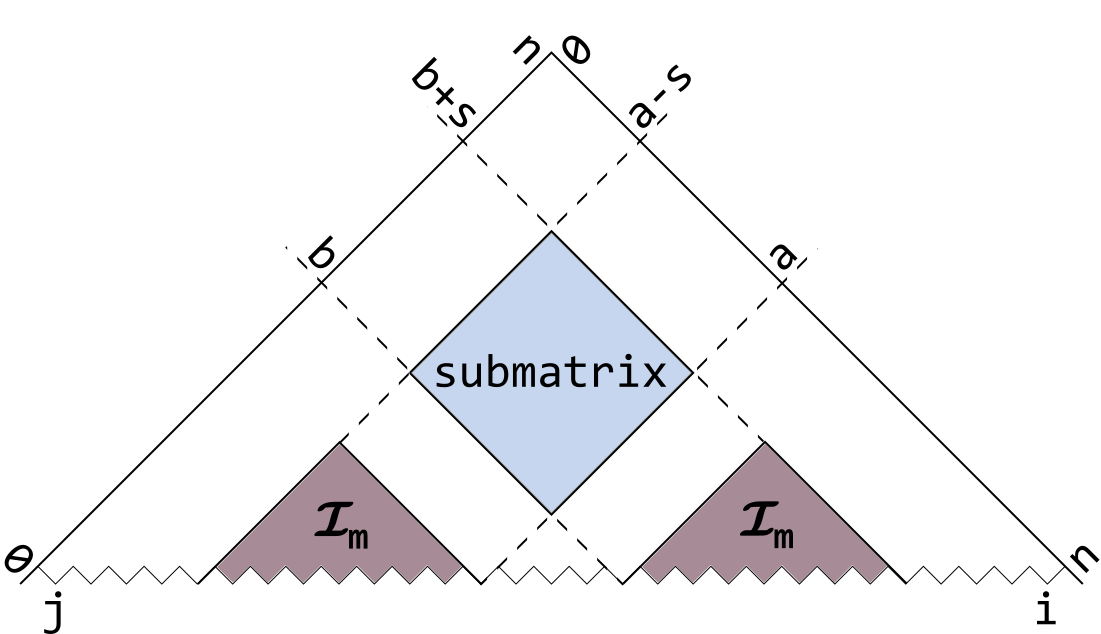
\includegraphics[width=0.7\linewidth]{part_02_Foundations/chapter_07_ClassicalParsing/figures/02_Valiant/submatrix.png}
  \caption{Иллюстрация к определению~\ref{def:ValiantSubmatrix}: $(a,b)$~--- вершина подматрицы $submatrix$ размером $s \times s$; $\mathcal{I}_m$~--- зона, влияющая на подматрицу $submatrix$}
  \label{fig:ValiantSubmatrix}
\end{figure}
\mytodo{Перевести в TikZ}

\begin{definition}[Влияющее множество]
  \label{def:ValiantInfluencing}
  Для подматрицы $m$ с вершиной $(a,b)$ и размером $s$ определим множество индексов $\mathcal{I}_m \subset \mathcal{I}$, \emph{влияющее на подматрицу $m$}, как:
  \[
    \mathcal{I}_m = \{(i, j) \in \mathcal{I} \mid a - s < i \leqslant a \;\land\; j \leqslant b\} \;\cup\;
                     \{(i, j) \in \mathcal{I} \mid b \leqslant i < j \;\land\; j < b + s\}.
  \]
\end{definition}

Геометрически $\mathcal{I}_m$~--- это множество ячеек, лежащих левее и ниже подматрицы $m$ на треугольной таблице (см.~рис.~\ref{fig:ValiantSubmatrix}).

Для подматрицы $m$ будем обозначать через $T[m]$ и $P[m]$ соответствующие подматрицы таблиц $T$ и $P$, то есть значения этих таблиц на множестве индексов $m$.

\subsection{Вспомогательные функции}

Для оперирования подматрицами введём набор вспомогательных функций.
Пусть подматрица $m$ имеет вершину $(a,b)$ и размер $s$.

Функции $\operatorname{size}(m)$ и $\operatorname{bottomCell}(m)$ возвращают размер и вершину подматрицы $m$ соответственно.

Функция $\operatorname{shift}(m, i, j)$ возвращает подматрицу размера $s$ с вершиной $(a+i, b+j)$.
На значения $i$ и $j$ накладываются естественные ограничения, чтобы результирующая подматрица не выходила за границы $\mathcal{I}$.

Следующие четыре функции делят исходную подматрицу $m$ на четыре равные части, как показано на рисунке~\ref{fig:ValiantInner}:
\begin{itemize}
  \item $\operatorname{bottomSubmatrix}(m)$~--- нижняя левая четверть (ближайшая к диагонали);
  \item $\operatorname{leftSubmatrix}(m)$~--- верхняя левая четверть;
  \item $\operatorname{rightSubmatrix}(m)$~--- нижняя правая четверть;
  \item $\operatorname{topSubmatrix}(m)$~--- верхняя правая четверть.
\end{itemize}

Размер каждой из этих подматриц равен $s/2$.

\begin{figure}[h]
  \centering
  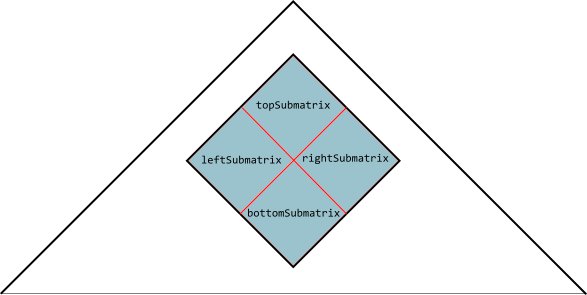
\includegraphics[width=0.7\linewidth]{part_02_Foundations/chapter_07_ClassicalParsing/figures/02_Valiant/inner.png}
  \caption{Разбиение подматрицы на четыре компоненты: $T$~--- top, $L$~--- left, $R$~--- right, $B$~--- bottom}
  \label{fig:ValiantInner}
\end{figure}
\mytodo{Перевести в TikZ}

Функции $\operatorname{rightNeighbor}(m)$ и $\operatorname{leftNeighbor}(m)$ возвращают подматрицы, сдвинутые относительно $m$ на $s$ по одной из осей (эквивалентны $\operatorname{shift}(m, s, 0)$ и $\operatorname{shift}(m, 0, -s)$ соответственно).

Функции $\operatorname{rightGrounded}(m)$ и $\operatorname{leftGrounded}(m)$ возвращают подматрицы, сдвинутые так, что их вершина $(i, j)$ лежит на главной <<диагонали>> $i + 1 = j$ (см.~рис.~\ref{fig:ValiantOuter}).
Они эквивалентны $\operatorname{shift}(m, b - a - 1, 0)$ и $\operatorname{shift}(m, 0, -(b - a - 1))$ соответственно.

\begin{figure}[h]
  \centering
  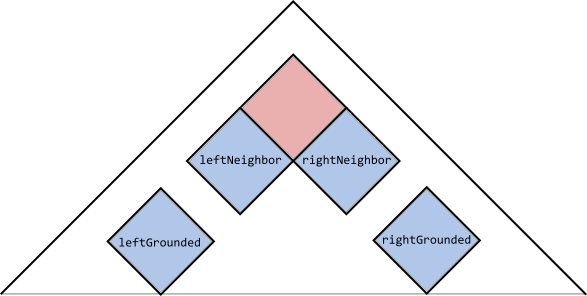
\includegraphics[width=0.7\linewidth]{part_02_Foundations/chapter_07_ClassicalParsing/figures/02_Valiant/outer.png}
  \caption{Иллюстрация функций $\operatorname{rightNeighbor}$, $\operatorname{leftNeighbor}$, $\operatorname{rightGrounded}$ и $\operatorname{leftGrounded}$}
  \label{fig:ValiantOuter}
\end{figure}
\mytodo{Перевести в TikZ}

\subsection{Умножение подматриц}

Центральная операция алгоритма~--- перемножение подматриц таблицы $T$.

\begin{definition}[Умножение подматриц]
  \label{def:ValiantMultiplication}
  Пусть $\mathcal{A}$ и $\mathcal{B}$~--- матрицы с элементами из $2^N$, причём $\mathcal{A}$ имеет размер $m \times k$, а $\mathcal{B}$~--- размер $k \times \ell$.
  Тогда результатом \emph{умножения} подматриц $\mathcal{A}$ и $\mathcal{B}$ является матрица $\mathcal{C} = \mathcal{A} \times \mathcal{B}$ размера $m \times \ell$ с элементами из $2^{N \times N}$, вычисляемыми по формуле:
  \[
    \mathcal{C}[i,j] = \{(A,B) \in N \times N \mid \exists r : A \in \mathcal{A}[i,r] \;\land\; B \in \mathcal{B}[r,j]\}.
  \]
\end{definition}

Заметим, что умножение $\mathcal{A} \times \mathcal{B}$ сводится к $|N|^2$ независимым умножениям булевых матриц: для каждой пары нетерминалов $(B, C) \in N \times N$ строится булева матрица $\mathcal{C}^{(B,C)}$, где $\mathcal{C}^{(B,C)}[i,j] = 1$ тогда и только тогда, когда $(B, C) \in \mathcal{C}[i,j]$, и при этом $\mathcal{C}^{(B,C)} = \mathcal{A}^{B} \times \mathcal{B}^{C}$, где $\mathcal{A}^{B}$ и $\mathcal{C}^{C}$~--- булевы матрицы, соответствующие нетерминалам $B$ и $C$.

Процедура $\operatorname{performMultiplications}$ принимает на вход множество троек $(m, m_1, m_2)$ и для каждой такой тройки выполняет умножение $T[m_1] \times T[m_2]$, добавляя результат в $P[m]$:
\begin{algorithm}[H]
  \caption{Процедура перемножения подматриц}
  \label{alg:ValiantPerformMultiplications}
  \textbf{procedure} $\operatorname{performMultiplications}(task)$:\;
  \ForEach{$(m, m_1, m_2) \in task$}{
    $P[m] \gets P[m] \cup (T[m_1] \times T[m_2])$\;
  }
\end{algorithm}

\subsection{Основной алгоритм}

Алгоритм~\ref{alg:ValiantMain} реализует синтаксический анализ через рекурсивное разбиение таблицы $T$ на подматрицы и их перемножение.
Процедура $\operatorname{compute}(i, j)$ рекурсивно делит интервал пополам и затем строит подматрицу с центром в точке деления.
Процедура $\operatorname{complete}(m)$ заполняет значения $T$ для всех ячеек подматрицы $m$, рекурсивно обрабатывая её четверти в определённом порядке с промежуточными умножениями.

\begin{algorithm}[H]
  \caption{Алгоритм синтаксического анализа, основанный на перемножении матриц}
  \label{alg:ValiantMain}
  \KwData{Грамматика $G = \langle N, \Sigma, R, S \rangle$ в НФХ, строка $w = a_1 \dots a_n$, где $n + 1 = 2^k$}

  \textbf{procedure} $\operatorname{main}()$:\;
    $\operatorname{compute}(n+1, n+1)$\;

  \BlankLine
  \textbf{procedure} $\operatorname{compute}(i, j)$:\;
    \If{$j - i \geqslant 4$}{
      $\operatorname{compute}(i, \frac{i+j}{2})$\;
      $\operatorname{compute}(\frac{i+j}{2}, j)$\;
    }
    $m \gets \operatorname{submatrixByBottomCellAndSize}((\frac{i+j}{2}-1, \frac{i+j}{2}), \frac{j-i}{2})$\;
    $\operatorname{complete}(m)$\;

  \BlankLine
  \textbf{procedure} $\operatorname{complete}(m)$:\;
    $(i, j) \gets \operatorname{bottomCell}(m)$\;
    \If{$\operatorname{size}(m) = 1$ \textbf{and} $i + 1 = j$}{
      $T[i,j] \gets \{A \mid A \to a_j \in R\}$\;
    }
    \ElseIf{$\operatorname{size}(m) = 1$}{
      $T[i,j] \gets \{A \mid \exists (B,C) \in P[i,j] : A \to BC \in R\}$\;
    }
    \Else{
      $\mathcal{B} \gets \operatorname{bottomSubmatrix}(m)$,
      $\mathcal{L} \gets \operatorname{leftSubmatrix}(m)$,
      $\mathcal{R} \gets \operatorname{rightSubmatrix}(m)$,
      $\mathcal{T} \gets \operatorname{topSubmatrix}(m)$\;
      $\operatorname{complete}(\mathcal{B})$\;
      $\operatorname{performMultiplications}(\{(\mathcal{L}, \operatorname{leftGrounded}(\mathcal{L}), \mathcal{B})\})$\;
      $\operatorname{complete}(\mathcal{L})$\;
      $\operatorname{performMultiplications}(\{(\mathcal{R}, \mathcal{B}, \operatorname{rightGrounded}(\mathcal{R}))\})$\;
      $\operatorname{complete}(\mathcal{R})$\;
      $\operatorname{performMultiplications}(\{(\mathcal{T}, \operatorname{leftGrounded}(\mathcal{T}), \mathcal{R})\})$\;
      $\operatorname{performMultiplications}(\{(\mathcal{T}, \mathcal{L}, \operatorname{rightGrounded}(\mathcal{T}))\})$\;
      $\operatorname{complete}(\mathcal{T})$\;
    }
\end{algorithm}

Разберём работу алгоритма подробнее.
Процедура $\operatorname{compute}(i, j)$ строит матрицу $T$ для всех ячеек $(i', j')$ таких, что $i' \geqslant i$ и $j' < j$.
Если длина интервала достаточно велика ($j - i \geqslant 4$), она рекурсивно делит его пополам, а затем с помощью $\operatorname{complete}$ заполняет подматрицу с вершиной в центре разбиения.

Процедура $\operatorname{complete}(m)$ определена для подматриц, размер которых является степенью двойки.
Она требует, чтобы $T$ уже была заполнена для всех ячеек из влияющего множества $\mathcal{I}_m$, а текущие значения $P[i,j]$ для $(i,j) \in m$ содержали все пары $(B,C)$, для которых разбиение подстроки $a_{i+1} \dots a_j$ некоторой промежуточной позицией $k$ между $a$ и $b$ даёт $a_{i+1} \dots a_k \in L_G(B)$ и $a_{k+1} \dots a_j \in L_G(C)$, где $(a,b)$~--- вершина $m$.

Для подматрицы размера $1$ с $i + 1 = j$ (ячейка на главной диагонали) заполнение происходит непосредственно из терминальных правил грамматики.
Для подматрицы размера $1$ с $i + 1 \neq j$ нетерминалы восстанавливаются из ранее заполненной матрицы $P$.
Для подматриц большего размера происходит рекурсивное деление на четыре четверти и четыре умножения в порядке, гарантирующем, что все необходимые данные будут готовы к моменту использования:
\begin{enumerate}
  \item Сначала полностью заполняется нижняя четверть $\mathcal{B}$ (рекурсивный вызов $\operatorname{complete}(\mathcal{B})$).
  \item Затем с помощью умножения <<заземлённой>> левой и $\mathcal{B}$ заполняется $P$ для левой четверти $\mathcal{L}$, после чего $\mathcal{L}$ заполняется рекурсивно.
  \item Аналогично, умножение $\mathcal{B}$ на <<заземлённую>> правую позволяет заполнить $P$ для правой четверти $\mathcal{R}$, после чего вызывается $\operatorname{complete}(\mathcal{R})$.
  \item Наконец, два умножения (<<заземлённая>> левая на $\mathcal{R}$ и $\mathcal{L}$ на <<заземлённую>> правую) заполняют $P$ для верхней четверти $\mathcal{T}$, после чего $\operatorname{complete}(\mathcal{T})$ завершает обработку.
\end{enumerate}

\subsection{Пример}

\begin{example}
  \label{exmpl:Valiant}
  Проиллюстрируем работу алгоритма Валианта на грамматике
  \begin{alignat*}{3}
  1) \ & S &&\rightarrow \varepsilon \\
  2) \ & S &&\rightarrow S\ S \\
  3) \ & S &&\rightarrow a\ S\ b \\
  \end{alignat*}
  и строке $w$ длины $6$
  \[
  \begin{pNiceMatrix}[margin=2pt] a & b & a & b & a & b \end{pNiceMatrix}
  \]
  Приведём грамматику к НФХ (раздел~\ref{sec:CNF}): терминалы $a$ и $b$ выносятся в отдельные продукции $N_3 \to a$ и $N_4 \to b$, правило $S \to a S b$ бинаризуется введением нового нетерминала $N_1$, а поскольку стартовый нетерминал $S$ выводит $\varepsilon$, вводится новый стартовый нетерминал $N_2$:
  \begin{alignat*}{3}
  1) \ & N_2 &&\rightarrow \varepsilon \\
  2) \ & N_2 &&\rightarrow S\ S \\
  3) \ & N_2 &&\rightarrow N_3\ N_1 \\
  4) \ & N_3 &&\rightarrow a \\
  5) \ & N_4 &&\rightarrow b \\
  6) \ & N_1 &&\rightarrow S\ N_4 \\
  7) \ & N_1 &&\rightarrow b \\
  8) \ & S &&\rightarrow S\ S \\
  9) \ & S &&\rightarrow N_3\ N_1 \\
  \end{alignat*}

  Длина строки равна $6$, поэтому $n + 1 = 7$ не является степенью двойки; таблица дополняется до размера $8 \times 8$, и использованной оказывается только верхнетреугольная часть, отвечающая позициям $0 \rng 6$ (последние строка и столбец не используются).
  На диагонали таблица инициализируется непосредственно из терминальных продукций: клетка $(0,1)$ содержит $N_3$ (символ $a$), клетка $(1,2)$~--- нетерминалы $N_1$ и $N_4$ (символ $b$), и так далее.

  Ниже приведены состояния таблицы $T$ после каждого из $28$ умножений.
  Пустая клетка обозначена $\cdot$; красным выделена подматрица $m$, в которую записывается произведение, синим и зелёным~--- две перемножаемые подматрицы, а жёлтым~--- клетки, изменившиеся на данном шаге.

\begin{center}
\begin{minipage}{0.49\linewidth}
\centering
\begin{adjustbox}{max width=\linewidth}
$
\begin{pNiceMatrix}[first-row,code-for-first-row = \arabic{jCol},first-col,code-for-first-col = \arabic{iRow}]
\CodeBefore
\rectanglecolor{red!10}{1-3}{1-3}
\rectanglecolor{blue!20}{1-2}{1-2}
\rectanglecolor{green!20}{2-3}{2-3}
\Body
 &  &  &  &  &  &  &  &  \\
 & \cdot & \{N_3\} & \cellcolor{yellow}{\{N_2, S\}} & \cdot & \cdot & \cdot & \cdot & \cdot \\
 & \cdot & \cdot & \{N_1, N_4\} & \cdot & \cdot & \cdot & \cdot & \cdot \\
 & \cdot & \cdot & \cdot & \{N_3\} & \cdot & \cdot & \cdot & \cdot \\
 & \cdot & \cdot & \cdot & \cdot & \{N_1, N_4\} & \cdot & \cdot & \cdot \\
 & \cdot & \cdot & \cdot & \cdot & \cdot & \{N_3\} & \cdot & \cdot \\
 & \cdot & \cdot & \cdot & \cdot & \cdot & \cdot & \{N_1, N_4\} & \cdot \\
 & \cdot & \cdot & \cdot & \cdot & \cdot & \cdot & \cdot & \cdot \\
 & \cdot & \cdot & \cdot & \cdot & \cdot & \cdot & \cdot & \cdot \\
\end{pNiceMatrix}
$
\end{adjustbox}
\end{minipage}
\hfill
\begin{minipage}{0.49\linewidth}
\centering
\begin{adjustbox}{max width=\linewidth}
$
\begin{pNiceMatrix}[first-row,code-for-first-row = \arabic{jCol},first-col,code-for-first-col = \arabic{iRow}]
\CodeBefore
\rectanglecolor{red!10}{2-4}{2-4}
\rectanglecolor{blue!20}{2-3}{2-3}
\rectanglecolor{green!20}{3-4}{3-4}
\Body
 &  &  &  &  &  &  &  &  \\
 & \cdot & \{N_3\} & \{N_2, S\} & \cdot & \cdot & \cdot & \cdot & \cdot \\
 & \cdot & \cdot & \{N_1, N_4\} & \cdot & \cdot & \cdot & \cdot & \cdot \\
 & \cdot & \cdot & \cdot & \{N_3\} & \cdot & \cdot & \cdot & \cdot \\
 & \cdot & \cdot & \cdot & \cdot & \{N_1, N_4\} & \cdot & \cdot & \cdot \\
 & \cdot & \cdot & \cdot & \cdot & \cdot & \{N_3\} & \cdot & \cdot \\
 & \cdot & \cdot & \cdot & \cdot & \cdot & \cdot & \{N_1, N_4\} & \cdot \\
 & \cdot & \cdot & \cdot & \cdot & \cdot & \cdot & \cdot & \cdot \\
 & \cdot & \cdot & \cdot & \cdot & \cdot & \cdot & \cdot & \cdot \\
\end{pNiceMatrix}
$
\end{adjustbox}
\end{minipage}
\end{center}
\begin{center}
\begin{minipage}{0.49\linewidth}
\centering
\begin{adjustbox}{max width=\linewidth}
$
\begin{pNiceMatrix}[first-row,code-for-first-row = \arabic{jCol},first-col,code-for-first-col = \arabic{iRow}]
\CodeBefore
\rectanglecolor{red!10}{1-4}{1-4}
\rectanglecolor{blue!20}{1-2}{1-2}
\rectanglecolor{green!20}{2-4}{2-4}
\Body
 &  &  &  &  &  &  &  &  \\
 & \cdot & \{N_3\} & \{N_2, S\} & \cdot & \cdot & \cdot & \cdot & \cdot \\
 & \cdot & \cdot & \{N_1, N_4\} & \cdot & \cdot & \cdot & \cdot & \cdot \\
 & \cdot & \cdot & \cdot & \{N_3\} & \cdot & \cdot & \cdot & \cdot \\
 & \cdot & \cdot & \cdot & \cdot & \{N_1, N_4\} & \cdot & \cdot & \cdot \\
 & \cdot & \cdot & \cdot & \cdot & \cdot & \{N_3\} & \cdot & \cdot \\
 & \cdot & \cdot & \cdot & \cdot & \cdot & \cdot & \{N_1, N_4\} & \cdot \\
 & \cdot & \cdot & \cdot & \cdot & \cdot & \cdot & \cdot & \cdot \\
 & \cdot & \cdot & \cdot & \cdot & \cdot & \cdot & \cdot & \cdot \\
\end{pNiceMatrix}
$
\end{adjustbox}
\end{minipage}
\hfill
\begin{minipage}{0.49\linewidth}
\centering
\begin{adjustbox}{max width=\linewidth}
$
\begin{pNiceMatrix}[first-row,code-for-first-row = \arabic{jCol},first-col,code-for-first-col = \arabic{iRow}]
\CodeBefore
\rectanglecolor{red!10}{1-4}{1-4}
\rectanglecolor{blue!20}{1-3}{1-3}
\rectanglecolor{green!20}{3-4}{3-4}
\Body
 &  &  &  &  &  &  &  &  \\
 & \cdot & \{N_3\} & \{N_2, S\} & \cdot & \cdot & \cdot & \cdot & \cdot \\
 & \cdot & \cdot & \{N_1, N_4\} & \cdot & \cdot & \cdot & \cdot & \cdot \\
 & \cdot & \cdot & \cdot & \{N_3\} & \cdot & \cdot & \cdot & \cdot \\
 & \cdot & \cdot & \cdot & \cdot & \{N_1, N_4\} & \cdot & \cdot & \cdot \\
 & \cdot & \cdot & \cdot & \cdot & \cdot & \{N_3\} & \cdot & \cdot \\
 & \cdot & \cdot & \cdot & \cdot & \cdot & \cdot & \{N_1, N_4\} & \cdot \\
 & \cdot & \cdot & \cdot & \cdot & \cdot & \cdot & \cdot & \cdot \\
 & \cdot & \cdot & \cdot & \cdot & \cdot & \cdot & \cdot & \cdot \\
\end{pNiceMatrix}
$
\end{adjustbox}
\end{minipage}
\end{center}
\begin{center}
\begin{minipage}{0.49\linewidth}
\centering
\begin{adjustbox}{max width=\linewidth}
$
\begin{pNiceMatrix}[first-row,code-for-first-row = \arabic{jCol},first-col,code-for-first-col = \arabic{iRow}]
\CodeBefore
\rectanglecolor{red!10}{5-7}{5-7}
\rectanglecolor{blue!20}{5-6}{5-6}
\rectanglecolor{green!20}{6-7}{6-7}
\Body
 &  &  &  &  &  &  &  &  \\
 & \cdot & \{N_3\} & \{N_2, S\} & \cdot & \cdot & \cdot & \cdot & \cdot \\
 & \cdot & \cdot & \{N_1, N_4\} & \cdot & \cdot & \cdot & \cdot & \cdot \\
 & \cdot & \cdot & \cdot & \{N_3\} & \cdot & \cdot & \cdot & \cdot \\
 & \cdot & \cdot & \cdot & \cdot & \{N_1, N_4\} & \cdot & \cdot & \cdot \\
 & \cdot & \cdot & \cdot & \cdot & \cdot & \{N_3\} & \cellcolor{yellow}{\{N_2, S\}} & \cdot \\
 & \cdot & \cdot & \cdot & \cdot & \cdot & \cdot & \{N_1, N_4\} & \cdot \\
 & \cdot & \cdot & \cdot & \cdot & \cdot & \cdot & \cdot & \cdot \\
 & \cdot & \cdot & \cdot & \cdot & \cdot & \cdot & \cdot & \cdot \\
\end{pNiceMatrix}
$
\end{adjustbox}
\end{minipage}
\hfill
\begin{minipage}{0.49\linewidth}
\centering
\begin{adjustbox}{max width=\linewidth}
$
\begin{pNiceMatrix}[first-row,code-for-first-row = \arabic{jCol},first-col,code-for-first-col = \arabic{iRow}]
\CodeBefore
\rectanglecolor{red!10}{6-8}{6-8}
\rectanglecolor{blue!20}{6-7}{6-7}
\rectanglecolor{green!20}{7-8}{7-8}
\Body
 &  &  &  &  &  &  &  &  \\
 & \cdot & \{N_3\} & \{N_2, S\} & \cdot & \cdot & \cdot & \cdot & \cdot \\
 & \cdot & \cdot & \{N_1, N_4\} & \cdot & \cdot & \cdot & \cdot & \cdot \\
 & \cdot & \cdot & \cdot & \{N_3\} & \cdot & \cdot & \cdot & \cdot \\
 & \cdot & \cdot & \cdot & \cdot & \{N_1, N_4\} & \cdot & \cdot & \cdot \\
 & \cdot & \cdot & \cdot & \cdot & \cdot & \{N_3\} & \{N_2, S\} & \cdot \\
 & \cdot & \cdot & \cdot & \cdot & \cdot & \cdot & \{N_1, N_4\} & \cdot \\
 & \cdot & \cdot & \cdot & \cdot & \cdot & \cdot & \cdot & \cdot \\
 & \cdot & \cdot & \cdot & \cdot & \cdot & \cdot & \cdot & \cdot \\
\end{pNiceMatrix}
$
\end{adjustbox}
\end{minipage}
\end{center}
\begin{center}
\begin{minipage}{0.49\linewidth}
\centering
\begin{adjustbox}{max width=\linewidth}
$
\begin{pNiceMatrix}[first-row,code-for-first-row = \arabic{jCol},first-col,code-for-first-col = \arabic{iRow}]
\CodeBefore
\rectanglecolor{red!10}{5-8}{5-8}
\rectanglecolor{blue!20}{5-6}{5-6}
\rectanglecolor{green!20}{6-8}{6-8}
\Body
 &  &  &  &  &  &  &  &  \\
 & \cdot & \{N_3\} & \{N_2, S\} & \cdot & \cdot & \cdot & \cdot & \cdot \\
 & \cdot & \cdot & \{N_1, N_4\} & \cdot & \cdot & \cdot & \cdot & \cdot \\
 & \cdot & \cdot & \cdot & \{N_3\} & \cdot & \cdot & \cdot & \cdot \\
 & \cdot & \cdot & \cdot & \cdot & \{N_1, N_4\} & \cdot & \cdot & \cdot \\
 & \cdot & \cdot & \cdot & \cdot & \cdot & \{N_3\} & \{N_2, S\} & \cdot \\
 & \cdot & \cdot & \cdot & \cdot & \cdot & \cdot & \{N_1, N_4\} & \cdot \\
 & \cdot & \cdot & \cdot & \cdot & \cdot & \cdot & \cdot & \cdot \\
 & \cdot & \cdot & \cdot & \cdot & \cdot & \cdot & \cdot & \cdot \\
\end{pNiceMatrix}
$
\end{adjustbox}
\end{minipage}
\hfill
\begin{minipage}{0.49\linewidth}
\centering
\begin{adjustbox}{max width=\linewidth}
$
\begin{pNiceMatrix}[first-row,code-for-first-row = \arabic{jCol},first-col,code-for-first-col = \arabic{iRow}]
\CodeBefore
\rectanglecolor{red!10}{5-8}{5-8}
\rectanglecolor{blue!20}{5-7}{5-7}
\rectanglecolor{green!20}{7-8}{7-8}
\Body
 &  &  &  &  &  &  &  &  \\
 & \cdot & \{N_3\} & \{N_2, S\} & \cdot & \cdot & \cdot & \cdot & \cdot \\
 & \cdot & \cdot & \{N_1, N_4\} & \cdot & \cdot & \cdot & \cdot & \cdot \\
 & \cdot & \cdot & \cdot & \{N_3\} & \cdot & \cdot & \cdot & \cdot \\
 & \cdot & \cdot & \cdot & \cdot & \{N_1, N_4\} & \cdot & \cdot & \cdot \\
 & \cdot & \cdot & \cdot & \cdot & \cdot & \{N_3\} & \{N_2, S\} & \cdot \\
 & \cdot & \cdot & \cdot & \cdot & \cdot & \cdot & \{N_1, N_4\} & \cdot \\
 & \cdot & \cdot & \cdot & \cdot & \cdot & \cdot & \cdot & \cdot \\
 & \cdot & \cdot & \cdot & \cdot & \cdot & \cdot & \cdot & \cdot \\
\end{pNiceMatrix}
$
\end{adjustbox}
\end{minipage}
\end{center}
\begin{center}
\begin{minipage}{0.49\linewidth}
\centering
\begin{adjustbox}{max width=\linewidth}
$
\begin{pNiceMatrix}[first-row,code-for-first-row = \arabic{jCol},first-col,code-for-first-col = \arabic{iRow}]
\CodeBefore
\rectanglecolor{red!10}{3-5}{3-5}
\rectanglecolor{blue!20}{3-4}{3-4}
\rectanglecolor{green!20}{4-5}{4-5}
\Body
 &  &  &  &  &  &  &  &  \\
 & \cdot & \{N_3\} & \{N_2, S\} & \cdot & \cdot & \cdot & \cdot & \cdot \\
 & \cdot & \cdot & \{N_1, N_4\} & \cdot & \cdot & \cdot & \cdot & \cdot \\
 & \cdot & \cdot & \cdot & \{N_3\} & \cellcolor{yellow}{\{N_2, S\}} & \cdot & \cdot & \cdot \\
 & \cdot & \cdot & \cdot & \cdot & \{N_1, N_4\} & \cdot & \cdot & \cdot \\
 & \cdot & \cdot & \cdot & \cdot & \cdot & \{N_3\} & \{N_2, S\} & \cdot \\
 & \cdot & \cdot & \cdot & \cdot & \cdot & \cdot & \{N_1, N_4\} & \cdot \\
 & \cdot & \cdot & \cdot & \cdot & \cdot & \cdot & \cdot & \cdot \\
 & \cdot & \cdot & \cdot & \cdot & \cdot & \cdot & \cdot & \cdot \\
\end{pNiceMatrix}
$
\end{adjustbox}
\end{minipage}
\hfill
\begin{minipage}{0.49\linewidth}
\centering
\begin{adjustbox}{max width=\linewidth}
$
\begin{pNiceMatrix}[first-row,code-for-first-row = \arabic{jCol},first-col,code-for-first-col = \arabic{iRow}]
\CodeBefore
\rectanglecolor{red!10}{4-6}{4-6}
\rectanglecolor{blue!20}{4-5}{4-5}
\rectanglecolor{green!20}{5-6}{5-6}
\Body
 &  &  &  &  &  &  &  &  \\
 & \cdot & \{N_3\} & \{N_2, S\} & \cdot & \cdot & \cdot & \cdot & \cdot \\
 & \cdot & \cdot & \{N_1, N_4\} & \cdot & \cdot & \cdot & \cdot & \cdot \\
 & \cdot & \cdot & \cdot & \{N_3\} & \{N_2, S\} & \cdot & \cdot & \cdot \\
 & \cdot & \cdot & \cdot & \cdot & \{N_1, N_4\} & \cdot & \cdot & \cdot \\
 & \cdot & \cdot & \cdot & \cdot & \cdot & \{N_3\} & \{N_2, S\} & \cdot \\
 & \cdot & \cdot & \cdot & \cdot & \cdot & \cdot & \{N_1, N_4\} & \cdot \\
 & \cdot & \cdot & \cdot & \cdot & \cdot & \cdot & \cdot & \cdot \\
 & \cdot & \cdot & \cdot & \cdot & \cdot & \cdot & \cdot & \cdot \\
\end{pNiceMatrix}
$
\end{adjustbox}
\end{minipage}
\end{center}
\begin{center}
\begin{minipage}{0.49\linewidth}
\centering
\begin{adjustbox}{max width=\linewidth}
$
\begin{pNiceMatrix}[first-row,code-for-first-row = \arabic{jCol},first-col,code-for-first-col = \arabic{iRow}]
\CodeBefore
\rectanglecolor{red!10}{3-6}{3-6}
\rectanglecolor{blue!20}{3-4}{3-4}
\rectanglecolor{green!20}{4-6}{4-6}
\Body
 &  &  &  &  &  &  &  &  \\
 & \cdot & \{N_3\} & \{N_2, S\} & \cdot & \cdot & \cdot & \cdot & \cdot \\
 & \cdot & \cdot & \{N_1, N_4\} & \cdot & \cdot & \cdot & \cdot & \cdot \\
 & \cdot & \cdot & \cdot & \{N_3\} & \{N_2, S\} & \cdot & \cdot & \cdot \\
 & \cdot & \cdot & \cdot & \cdot & \{N_1, N_4\} & \cdot & \cdot & \cdot \\
 & \cdot & \cdot & \cdot & \cdot & \cdot & \{N_3\} & \{N_2, S\} & \cdot \\
 & \cdot & \cdot & \cdot & \cdot & \cdot & \cdot & \{N_1, N_4\} & \cdot \\
 & \cdot & \cdot & \cdot & \cdot & \cdot & \cdot & \cdot & \cdot \\
 & \cdot & \cdot & \cdot & \cdot & \cdot & \cdot & \cdot & \cdot \\
\end{pNiceMatrix}
$
\end{adjustbox}
\end{minipage}
\hfill
\begin{minipage}{0.49\linewidth}
\centering
\begin{adjustbox}{max width=\linewidth}
$
\begin{pNiceMatrix}[first-row,code-for-first-row = \arabic{jCol},first-col,code-for-first-col = \arabic{iRow}]
\CodeBefore
\rectanglecolor{red!10}{3-6}{3-6}
\rectanglecolor{blue!20}{3-5}{3-5}
\rectanglecolor{green!20}{5-6}{5-6}
\Body
 &  &  &  &  &  &  &  &  \\
 & \cdot & \{N_3\} & \{N_2, S\} & \cdot & \cdot & \cdot & \cdot & \cdot \\
 & \cdot & \cdot & \{N_1, N_4\} & \cdot & \cdot & \cdot & \cdot & \cdot \\
 & \cdot & \cdot & \cdot & \{N_3\} & \{N_2, S\} & \cdot & \cdot & \cdot \\
 & \cdot & \cdot & \cdot & \cdot & \{N_1, N_4\} & \cdot & \cdot & \cdot \\
 & \cdot & \cdot & \cdot & \cdot & \cdot & \{N_3\} & \{N_2, S\} & \cdot \\
 & \cdot & \cdot & \cdot & \cdot & \cdot & \cdot & \{N_1, N_4\} & \cdot \\
 & \cdot & \cdot & \cdot & \cdot & \cdot & \cdot & \cdot & \cdot \\
 & \cdot & \cdot & \cdot & \cdot & \cdot & \cdot & \cdot & \cdot \\
\end{pNiceMatrix}
$
\end{adjustbox}
\end{minipage}
\end{center}
\begin{center}
\begin{minipage}{0.49\linewidth}
\centering
\begin{adjustbox}{max width=\linewidth}
$
\begin{pNiceMatrix}[first-row,code-for-first-row = \arabic{jCol},first-col,code-for-first-col = \arabic{iRow}]
\CodeBefore
\rectanglecolor{red!10}{1-5}{2-6}
\rectanglecolor{blue!20}{1-3}{2-4}
\rectanglecolor{green!20}{3-5}{4-6}
\Body
 &  &  &  &  &  &  &  &  \\
 & \cdot & \{N_3\} & \{N_2, S\} & \cdot & \cellcolor{yellow}{\{N_2, S\}} & \cdot & \cdot & \cdot \\
 & \cdot & \cdot & \{N_1, N_4\} & \cdot & \cdot & \cdot & \cdot & \cdot \\
 & \cdot & \cdot & \cdot & \{N_3\} & \{N_2, S\} & \cdot & \cdot & \cdot \\
 & \cdot & \cdot & \cdot & \cdot & \{N_1, N_4\} & \cdot & \cdot & \cdot \\
 & \cdot & \cdot & \cdot & \cdot & \cdot & \{N_3\} & \{N_2, S\} & \cdot \\
 & \cdot & \cdot & \cdot & \cdot & \cdot & \cdot & \{N_1, N_4\} & \cdot \\
 & \cdot & \cdot & \cdot & \cdot & \cdot & \cdot & \cdot & \cdot \\
 & \cdot & \cdot & \cdot & \cdot & \cdot & \cdot & \cdot & \cdot \\
\end{pNiceMatrix}
$
\end{adjustbox}
\end{minipage}
\hfill
\begin{minipage}{0.49\linewidth}
\centering
\begin{adjustbox}{max width=\linewidth}
$
\begin{pNiceMatrix}[first-row,code-for-first-row = \arabic{jCol},first-col,code-for-first-col = \arabic{iRow}]
\CodeBefore
\rectanglecolor{red!10}{1-5}{1-5}
\rectanglecolor{blue!20}{1-2}{1-2}
\rectanglecolor{green!20}{2-5}{2-5}
\Body
 &  &  &  &  &  &  &  &  \\
 & \cdot & \{N_3\} & \{N_2, S\} & \cdot & \{N_2, S\} & \cdot & \cdot & \cdot \\
 & \cdot & \cdot & \{N_1, N_4\} & \cdot & \cdot & \cdot & \cdot & \cdot \\
 & \cdot & \cdot & \cdot & \{N_3\} & \{N_2, S\} & \cdot & \cdot & \cdot \\
 & \cdot & \cdot & \cdot & \cdot & \{N_1, N_4\} & \cdot & \cdot & \cdot \\
 & \cdot & \cdot & \cdot & \cdot & \cdot & \{N_3\} & \{N_2, S\} & \cdot \\
 & \cdot & \cdot & \cdot & \cdot & \cdot & \cdot & \{N_1, N_4\} & \cdot \\
 & \cdot & \cdot & \cdot & \cdot & \cdot & \cdot & \cdot & \cdot \\
 & \cdot & \cdot & \cdot & \cdot & \cdot & \cdot & \cdot & \cdot \\
\end{pNiceMatrix}
$
\end{adjustbox}
\end{minipage}
\end{center}
\begin{center}
\begin{minipage}{0.49\linewidth}
\centering
\begin{adjustbox}{max width=\linewidth}
$
\begin{pNiceMatrix}[first-row,code-for-first-row = \arabic{jCol},first-col,code-for-first-col = \arabic{iRow}]
\CodeBefore
\rectanglecolor{red!10}{2-6}{2-6}
\rectanglecolor{blue!20}{2-5}{2-5}
\rectanglecolor{green!20}{5-6}{5-6}
\Body
 &  &  &  &  &  &  &  &  \\
 & \cdot & \{N_3\} & \{N_2, S\} & \cdot & \{N_2, S\} & \cdot & \cdot & \cdot \\
 & \cdot & \cdot & \{N_1, N_4\} & \cdot & \cdot & \cdot & \cdot & \cdot \\
 & \cdot & \cdot & \cdot & \{N_3\} & \{N_2, S\} & \cdot & \cdot & \cdot \\
 & \cdot & \cdot & \cdot & \cdot & \{N_1, N_4\} & \cdot & \cdot & \cdot \\
 & \cdot & \cdot & \cdot & \cdot & \cdot & \{N_3\} & \{N_2, S\} & \cdot \\
 & \cdot & \cdot & \cdot & \cdot & \cdot & \cdot & \{N_1, N_4\} & \cdot \\
 & \cdot & \cdot & \cdot & \cdot & \cdot & \cdot & \cdot & \cdot \\
 & \cdot & \cdot & \cdot & \cdot & \cdot & \cdot & \cdot & \cdot \\
\end{pNiceMatrix}
$
\end{adjustbox}
\end{minipage}
\hfill
\begin{minipage}{0.49\linewidth}
\centering
\begin{adjustbox}{max width=\linewidth}
$
\begin{pNiceMatrix}[first-row,code-for-first-row = \arabic{jCol},first-col,code-for-first-col = \arabic{iRow}]
\CodeBefore
\rectanglecolor{red!10}{1-6}{1-6}
\rectanglecolor{blue!20}{1-2}{1-2}
\rectanglecolor{green!20}{2-6}{2-6}
\Body
 &  &  &  &  &  &  &  &  \\
 & \cdot & \{N_3\} & \{N_2, S\} & \cdot & \{N_2, S\} & \cdot & \cdot & \cdot \\
 & \cdot & \cdot & \{N_1, N_4\} & \cdot & \cdot & \cdot & \cdot & \cdot \\
 & \cdot & \cdot & \cdot & \{N_3\} & \{N_2, S\} & \cdot & \cdot & \cdot \\
 & \cdot & \cdot & \cdot & \cdot & \{N_1, N_4\} & \cdot & \cdot & \cdot \\
 & \cdot & \cdot & \cdot & \cdot & \cdot & \{N_3\} & \{N_2, S\} & \cdot \\
 & \cdot & \cdot & \cdot & \cdot & \cdot & \cdot & \{N_1, N_4\} & \cdot \\
 & \cdot & \cdot & \cdot & \cdot & \cdot & \cdot & \cdot & \cdot \\
 & \cdot & \cdot & \cdot & \cdot & \cdot & \cdot & \cdot & \cdot \\
\end{pNiceMatrix}
$
\end{adjustbox}
\end{minipage}
\end{center}
\begin{center}
\begin{minipage}{0.49\linewidth}
\centering
\begin{adjustbox}{max width=\linewidth}
$
\begin{pNiceMatrix}[first-row,code-for-first-row = \arabic{jCol},first-col,code-for-first-col = \arabic{iRow}]
\CodeBefore
\rectanglecolor{red!10}{1-6}{1-6}
\rectanglecolor{blue!20}{1-5}{1-5}
\rectanglecolor{green!20}{5-6}{5-6}
\Body
 &  &  &  &  &  &  &  &  \\
 & \cdot & \{N_3\} & \{N_2, S\} & \cdot & \{N_2, S\} & \cdot & \cdot & \cdot \\
 & \cdot & \cdot & \{N_1, N_4\} & \cdot & \cdot & \cdot & \cdot & \cdot \\
 & \cdot & \cdot & \cdot & \{N_3\} & \{N_2, S\} & \cdot & \cdot & \cdot \\
 & \cdot & \cdot & \cdot & \cdot & \{N_1, N_4\} & \cdot & \cdot & \cdot \\
 & \cdot & \cdot & \cdot & \cdot & \cdot & \{N_3\} & \{N_2, S\} & \cdot \\
 & \cdot & \cdot & \cdot & \cdot & \cdot & \cdot & \{N_1, N_4\} & \cdot \\
 & \cdot & \cdot & \cdot & \cdot & \cdot & \cdot & \cdot & \cdot \\
 & \cdot & \cdot & \cdot & \cdot & \cdot & \cdot & \cdot & \cdot \\
\end{pNiceMatrix}
$
\end{adjustbox}
\end{minipage}
\hfill
\begin{minipage}{0.49\linewidth}
\centering
\begin{adjustbox}{max width=\linewidth}
$
\begin{pNiceMatrix}[first-row,code-for-first-row = \arabic{jCol},first-col,code-for-first-col = \arabic{iRow}]
\CodeBefore
\rectanglecolor{red!10}{3-7}{4-8}
\rectanglecolor{blue!20}{3-5}{4-6}
\rectanglecolor{green!20}{5-7}{6-8}
\Body
 &  &  &  &  &  &  &  &  \\
 & \cdot & \{N_3\} & \{N_2, S\} & \cdot & \{N_2, S\} & \cdot & \cdot & \cdot \\
 & \cdot & \cdot & \{N_1, N_4\} & \cdot & \cdot & \cdot & \cdot & \cdot \\
 & \cdot & \cdot & \cdot & \{N_3\} & \{N_2, S\} & \cdot & \cellcolor{yellow}{\{N_2, S\}} & \cdot \\
 & \cdot & \cdot & \cdot & \cdot & \{N_1, N_4\} & \cdot & \cdot & \cdot \\
 & \cdot & \cdot & \cdot & \cdot & \cdot & \{N_3\} & \{N_2, S\} & \cdot \\
 & \cdot & \cdot & \cdot & \cdot & \cdot & \cdot & \{N_1, N_4\} & \cdot \\
 & \cdot & \cdot & \cdot & \cdot & \cdot & \cdot & \cdot & \cdot \\
 & \cdot & \cdot & \cdot & \cdot & \cdot & \cdot & \cdot & \cdot \\
\end{pNiceMatrix}
$
\end{adjustbox}
\end{minipage}
\end{center}
\begin{center}
\begin{minipage}{0.49\linewidth}
\centering
\begin{adjustbox}{max width=\linewidth}
$
\begin{pNiceMatrix}[first-row,code-for-first-row = \arabic{jCol},first-col,code-for-first-col = \arabic{iRow}]
\CodeBefore
\rectanglecolor{red!10}{3-7}{3-7}
\rectanglecolor{blue!20}{3-4}{3-4}
\rectanglecolor{green!20}{4-7}{4-7}
\Body
 &  &  &  &  &  &  &  &  \\
 & \cdot & \{N_3\} & \{N_2, S\} & \cdot & \{N_2, S\} & \cdot & \cdot & \cdot \\
 & \cdot & \cdot & \{N_1, N_4\} & \cdot & \cdot & \cdot & \cdot & \cdot \\
 & \cdot & \cdot & \cdot & \{N_3\} & \{N_2, S\} & \cdot & \{N_2, S\} & \cdot \\
 & \cdot & \cdot & \cdot & \cdot & \{N_1, N_4\} & \cdot & \cdot & \cdot \\
 & \cdot & \cdot & \cdot & \cdot & \cdot & \{N_3\} & \{N_2, S\} & \cdot \\
 & \cdot & \cdot & \cdot & \cdot & \cdot & \cdot & \{N_1, N_4\} & \cdot \\
 & \cdot & \cdot & \cdot & \cdot & \cdot & \cdot & \cdot & \cdot \\
 & \cdot & \cdot & \cdot & \cdot & \cdot & \cdot & \cdot & \cdot \\
\end{pNiceMatrix}
$
\end{adjustbox}
\end{minipage}
\hfill
\begin{minipage}{0.49\linewidth}
\centering
\begin{adjustbox}{max width=\linewidth}
$
\begin{pNiceMatrix}[first-row,code-for-first-row = \arabic{jCol},first-col,code-for-first-col = \arabic{iRow}]
\CodeBefore
\rectanglecolor{red!10}{4-8}{4-8}
\rectanglecolor{blue!20}{4-7}{4-7}
\rectanglecolor{green!20}{7-8}{7-8}
\Body
 &  &  &  &  &  &  &  &  \\
 & \cdot & \{N_3\} & \{N_2, S\} & \cdot & \{N_2, S\} & \cdot & \cdot & \cdot \\
 & \cdot & \cdot & \{N_1, N_4\} & \cdot & \cdot & \cdot & \cdot & \cdot \\
 & \cdot & \cdot & \cdot & \{N_3\} & \{N_2, S\} & \cdot & \{N_2, S\} & \cdot \\
 & \cdot & \cdot & \cdot & \cdot & \{N_1, N_4\} & \cdot & \cdot & \cdot \\
 & \cdot & \cdot & \cdot & \cdot & \cdot & \{N_3\} & \{N_2, S\} & \cdot \\
 & \cdot & \cdot & \cdot & \cdot & \cdot & \cdot & \{N_1, N_4\} & \cdot \\
 & \cdot & \cdot & \cdot & \cdot & \cdot & \cdot & \cdot & \cdot \\
 & \cdot & \cdot & \cdot & \cdot & \cdot & \cdot & \cdot & \cdot \\
\end{pNiceMatrix}
$
\end{adjustbox}
\end{minipage}
\end{center}
\begin{center}
\begin{minipage}{0.49\linewidth}
\centering
\begin{adjustbox}{max width=\linewidth}
$
\begin{pNiceMatrix}[first-row,code-for-first-row = \arabic{jCol},first-col,code-for-first-col = \arabic{iRow}]
\CodeBefore
\rectanglecolor{red!10}{3-8}{3-8}
\rectanglecolor{blue!20}{3-4}{3-4}
\rectanglecolor{green!20}{4-8}{4-8}
\Body
 &  &  &  &  &  &  &  &  \\
 & \cdot & \{N_3\} & \{N_2, S\} & \cdot & \{N_2, S\} & \cdot & \cdot & \cdot \\
 & \cdot & \cdot & \{N_1, N_4\} & \cdot & \cdot & \cdot & \cdot & \cdot \\
 & \cdot & \cdot & \cdot & \{N_3\} & \{N_2, S\} & \cdot & \{N_2, S\} & \cdot \\
 & \cdot & \cdot & \cdot & \cdot & \{N_1, N_4\} & \cdot & \cdot & \cdot \\
 & \cdot & \cdot & \cdot & \cdot & \cdot & \{N_3\} & \{N_2, S\} & \cdot \\
 & \cdot & \cdot & \cdot & \cdot & \cdot & \cdot & \{N_1, N_4\} & \cdot \\
 & \cdot & \cdot & \cdot & \cdot & \cdot & \cdot & \cdot & \cdot \\
 & \cdot & \cdot & \cdot & \cdot & \cdot & \cdot & \cdot & \cdot \\
\end{pNiceMatrix}
$
\end{adjustbox}
\end{minipage}
\hfill
\begin{minipage}{0.49\linewidth}
\centering
\begin{adjustbox}{max width=\linewidth}
$
\begin{pNiceMatrix}[first-row,code-for-first-row = \arabic{jCol},first-col,code-for-first-col = \arabic{iRow}]
\CodeBefore
\rectanglecolor{red!10}{3-8}{3-8}
\rectanglecolor{blue!20}{3-7}{3-7}
\rectanglecolor{green!20}{7-8}{7-8}
\Body
 &  &  &  &  &  &  &  &  \\
 & \cdot & \{N_3\} & \{N_2, S\} & \cdot & \{N_2, S\} & \cdot & \cdot & \cdot \\
 & \cdot & \cdot & \{N_1, N_4\} & \cdot & \cdot & \cdot & \cdot & \cdot \\
 & \cdot & \cdot & \cdot & \{N_3\} & \{N_2, S\} & \cdot & \{N_2, S\} & \cdot \\
 & \cdot & \cdot & \cdot & \cdot & \{N_1, N_4\} & \cdot & \cdot & \cdot \\
 & \cdot & \cdot & \cdot & \cdot & \cdot & \{N_3\} & \{N_2, S\} & \cdot \\
 & \cdot & \cdot & \cdot & \cdot & \cdot & \cdot & \{N_1, N_4\} & \cdot \\
 & \cdot & \cdot & \cdot & \cdot & \cdot & \cdot & \cdot & \cdot \\
 & \cdot & \cdot & \cdot & \cdot & \cdot & \cdot & \cdot & \cdot \\
\end{pNiceMatrix}
$
\end{adjustbox}
\end{minipage}
\end{center}
\begin{center}
\begin{minipage}{0.49\linewidth}
\centering
\begin{adjustbox}{max width=\linewidth}
$
\begin{pNiceMatrix}[first-row,code-for-first-row = \arabic{jCol},first-col,code-for-first-col = \arabic{iRow}]
\CodeBefore
\rectanglecolor{red!10}{1-7}{2-8}
\rectanglecolor{blue!20}{1-3}{2-4}
\rectanglecolor{green!20}{3-7}{4-8}
\Body
 &  &  &  &  &  &  &  &  \\
 & \cdot & \{N_3\} & \{N_2, S\} & \cdot & \{N_2, S\} & \cdot & \cellcolor{yellow}{\{N_2, S\}} & \cdot \\
 & \cdot & \cdot & \{N_1, N_4\} & \cdot & \cdot & \cdot & \cdot & \cdot \\
 & \cdot & \cdot & \cdot & \{N_3\} & \{N_2, S\} & \cdot & \{N_2, S\} & \cdot \\
 & \cdot & \cdot & \cdot & \cdot & \{N_1, N_4\} & \cdot & \cdot & \cdot \\
 & \cdot & \cdot & \cdot & \cdot & \cdot & \{N_3\} & \{N_2, S\} & \cdot \\
 & \cdot & \cdot & \cdot & \cdot & \cdot & \cdot & \{N_1, N_4\} & \cdot \\
 & \cdot & \cdot & \cdot & \cdot & \cdot & \cdot & \cdot & \cdot \\
 & \cdot & \cdot & \cdot & \cdot & \cdot & \cdot & \cdot & \cdot \\
\end{pNiceMatrix}
$
\end{adjustbox}
\end{minipage}
\hfill
\begin{minipage}{0.49\linewidth}
\centering
\begin{adjustbox}{max width=\linewidth}
$
\begin{pNiceMatrix}[first-row,code-for-first-row = \arabic{jCol},first-col,code-for-first-col = \arabic{iRow}]
\CodeBefore
\rectanglecolor{red!10}{1-7}{2-8}
\rectanglecolor{blue!20}{1-5}{2-6}
\rectanglecolor{green!20}{5-7}{6-8}
\Body
 &  &  &  &  &  &  &  &  \\
 & \cdot & \{N_3\} & \{N_2, S\} & \cdot & \{N_2, S\} & \cdot & \cellcolor{yellow}{\{N_2, S\}} & \cdot \\
 & \cdot & \cdot & \{N_1, N_4\} & \cdot & \cdot & \cdot & \cdot & \cdot \\
 & \cdot & \cdot & \cdot & \{N_3\} & \{N_2, S\} & \cdot & \{N_2, S\} & \cdot \\
 & \cdot & \cdot & \cdot & \cdot & \{N_1, N_4\} & \cdot & \cdot & \cdot \\
 & \cdot & \cdot & \cdot & \cdot & \cdot & \{N_3\} & \{N_2, S\} & \cdot \\
 & \cdot & \cdot & \cdot & \cdot & \cdot & \cdot & \{N_1, N_4\} & \cdot \\
 & \cdot & \cdot & \cdot & \cdot & \cdot & \cdot & \cdot & \cdot \\
 & \cdot & \cdot & \cdot & \cdot & \cdot & \cdot & \cdot & \cdot \\
\end{pNiceMatrix}
$
\end{adjustbox}
\end{minipage}
\end{center}
\begin{center}
\begin{minipage}{0.49\linewidth}
\centering
\begin{adjustbox}{max width=\linewidth}
$
\begin{pNiceMatrix}[first-row,code-for-first-row = \arabic{jCol},first-col,code-for-first-col = \arabic{iRow}]
\CodeBefore
\rectanglecolor{red!10}{1-7}{1-7}
\rectanglecolor{blue!20}{1-2}{1-2}
\rectanglecolor{green!20}{2-7}{2-7}
\Body
 &  &  &  &  &  &  &  &  \\
 & \cdot & \{N_3\} & \{N_2, S\} & \cdot & \{N_2, S\} & \cdot & \{N_2, S\} & \cdot \\
 & \cdot & \cdot & \{N_1, N_4\} & \cdot & \cdot & \cdot & \cdot & \cdot \\
 & \cdot & \cdot & \cdot & \{N_3\} & \{N_2, S\} & \cdot & \{N_2, S\} & \cdot \\
 & \cdot & \cdot & \cdot & \cdot & \{N_1, N_4\} & \cdot & \cdot & \cdot \\
 & \cdot & \cdot & \cdot & \cdot & \cdot & \{N_3\} & \{N_2, S\} & \cdot \\
 & \cdot & \cdot & \cdot & \cdot & \cdot & \cdot & \{N_1, N_4\} & \cdot \\
 & \cdot & \cdot & \cdot & \cdot & \cdot & \cdot & \cdot & \cdot \\
 & \cdot & \cdot & \cdot & \cdot & \cdot & \cdot & \cdot & \cdot \\
\end{pNiceMatrix}
$
\end{adjustbox}
\end{minipage}
\hfill
\begin{minipage}{0.49\linewidth}
\centering
\begin{adjustbox}{max width=\linewidth}
$
\begin{pNiceMatrix}[first-row,code-for-first-row = \arabic{jCol},first-col,code-for-first-col = \arabic{iRow}]
\CodeBefore
\rectanglecolor{red!10}{2-8}{2-8}
\rectanglecolor{blue!20}{2-7}{2-7}
\rectanglecolor{green!20}{7-8}{7-8}
\Body
 &  &  &  &  &  &  &  &  \\
 & \cdot & \{N_3\} & \{N_2, S\} & \cdot & \{N_2, S\} & \cdot & \{N_2, S\} & \cdot \\
 & \cdot & \cdot & \{N_1, N_4\} & \cdot & \cdot & \cdot & \cdot & \cdot \\
 & \cdot & \cdot & \cdot & \{N_3\} & \{N_2, S\} & \cdot & \{N_2, S\} & \cdot \\
 & \cdot & \cdot & \cdot & \cdot & \{N_1, N_4\} & \cdot & \cdot & \cdot \\
 & \cdot & \cdot & \cdot & \cdot & \cdot & \{N_3\} & \{N_2, S\} & \cdot \\
 & \cdot & \cdot & \cdot & \cdot & \cdot & \cdot & \{N_1, N_4\} & \cdot \\
 & \cdot & \cdot & \cdot & \cdot & \cdot & \cdot & \cdot & \cdot \\
 & \cdot & \cdot & \cdot & \cdot & \cdot & \cdot & \cdot & \cdot \\
\end{pNiceMatrix}
$
\end{adjustbox}
\end{minipage}
\end{center}
\begin{center}
\begin{minipage}{0.49\linewidth}
\centering
\begin{adjustbox}{max width=\linewidth}
$
\begin{pNiceMatrix}[first-row,code-for-first-row = \arabic{jCol},first-col,code-for-first-col = \arabic{iRow}]
\CodeBefore
\rectanglecolor{red!10}{1-8}{1-8}
\rectanglecolor{blue!20}{1-2}{1-2}
\rectanglecolor{green!20}{2-8}{2-8}
\Body
 &  &  &  &  &  &  &  &  \\
 & \cdot & \{N_3\} & \{N_2, S\} & \cdot & \{N_2, S\} & \cdot & \{N_2, S\} & \cdot \\
 & \cdot & \cdot & \{N_1, N_4\} & \cdot & \cdot & \cdot & \cdot & \cdot \\
 & \cdot & \cdot & \cdot & \{N_3\} & \{N_2, S\} & \cdot & \{N_2, S\} & \cdot \\
 & \cdot & \cdot & \cdot & \cdot & \{N_1, N_4\} & \cdot & \cdot & \cdot \\
 & \cdot & \cdot & \cdot & \cdot & \cdot & \{N_3\} & \{N_2, S\} & \cdot \\
 & \cdot & \cdot & \cdot & \cdot & \cdot & \cdot & \{N_1, N_4\} & \cdot \\
 & \cdot & \cdot & \cdot & \cdot & \cdot & \cdot & \cdot & \cdot \\
 & \cdot & \cdot & \cdot & \cdot & \cdot & \cdot & \cdot & \cdot \\
\end{pNiceMatrix}
$
\end{adjustbox}
\end{minipage}
\hfill
\begin{minipage}{0.49\linewidth}
\centering
\begin{adjustbox}{max width=\linewidth}
$
\begin{pNiceMatrix}[first-row,code-for-first-row = \arabic{jCol},first-col,code-for-first-col = \arabic{iRow}]
\CodeBefore
\rectanglecolor{red!10}{1-8}{1-8}
\rectanglecolor{blue!20}{1-7}{1-7}
\rectanglecolor{green!20}{7-8}{7-8}
\Body
 &  &  &  &  &  &  &  &  \\
 & \cdot & \{N_3\} & \{N_2, S\} & \cdot & \{N_2, S\} & \cdot & \{N_2, S\} & \cdot \\
 & \cdot & \cdot & \{N_1, N_4\} & \cdot & \cdot & \cdot & \cdot & \cdot \\
 & \cdot & \cdot & \cdot & \{N_3\} & \{N_2, S\} & \cdot & \{N_2, S\} & \cdot \\
 & \cdot & \cdot & \cdot & \cdot & \{N_1, N_4\} & \cdot & \cdot & \cdot \\
 & \cdot & \cdot & \cdot & \cdot & \cdot & \{N_3\} & \{N_2, S\} & \cdot \\
 & \cdot & \cdot & \cdot & \cdot & \cdot & \cdot & \{N_1, N_4\} & \cdot \\
 & \cdot & \cdot & \cdot & \cdot & \cdot & \cdot & \cdot & \cdot \\
 & \cdot & \cdot & \cdot & \cdot & \cdot & \cdot & \cdot & \cdot \\
\end{pNiceMatrix}
$
\end{adjustbox}
\end{minipage}
\end{center}

  В клетке $T[0,6]$, соответствующей всей строке, оказывается нетерминал $S$ (наряду с вспомогательным $N_2$), следовательно, строка $a b a b a b$ выводима в грамматике.
\end{example}

\subsection{Вариант с восстановлением SPPF}

Описанный выше алгоритм решает задачу выводимости: в ячейках таблицы $T$ хранятся множества нетерминалов, а информация о том, как именно подстрока разбивается на части, отбрасывается.
Чтобы восстановить сжатое представление леса разбора (SPPF, раздел~\ref{sec:SPPF}) в варианте Рекерса (определение~\ref{def:basicSPPF}), достаточно хранить в ячейке таблицы $T$ вместо множества нетерминалов множество троек вида $(A, k, p)$, где $A$~--- нетерминал, $k$~--- точка расщепления, а $p$~--- номер продукции грамматики, приведённой к НФХ (так же, как в версии CYK с восстановлением SPPF, раздел~\ref{sec:lin_CYK}).
Тройка $(A, k, p)$ в клетке $T[i,j]$ означает, что нетерминал $A$ выводит подстроку $a_{i+1} \dots a_j$ продукцией с номером $p$; для бинарной продукции $A \to B C$ точка расщепления $k$ задаёт разбиение подстроки: $B$ выводит $a_{i+1} \dots a_{k+1}$, а $C$~--- $a_{k+2} \dots a_j$.

С алгебраической точки зрения переход к тройкам означает замену булева полукольца на полукольцо множеств троек: сложение~--- объединение множеств, а умножение склеивает тройки из перемножаемых матриц.
Однако обычного умножения над полукольцом недостаточно: точку расщепления необходимо <<вписать>> в тройку из промежуточного индекса перемножения.
Поэтому перемножение подматриц (определение~\ref{def:ValiantMultiplication}) заменяется индексной операцией, которой при вычислении элемента результата в клетке $(i,j)$ доступен промежуточный индекс $r$: именно он записывается в тройку как точка расщепления $k$.

\begin{example}
  \label{exmpl:Valiant_SPPF}
  Проиллюстрируем работу модифицированного алгоритма на неоднозначной грамматике
  \begin{alignat*}{3}
  1) \ & S &&\rightarrow a \\
  2) \ & S &&\rightarrow S\ S \\
  3) \ & S &&\rightarrow S\ S\ S \\
  \end{alignat*}
  и цепочке $w = a a a$.
  Приведём грамматику к НФХ (раздел~\ref{sec:CNF}): продукцию $S \to S S S$ длины три заменим на две бинарные продукции, введя новый нетерминал $N_1$:
  \begin{alignat*}{3}
  1) \ & S &&\rightarrow a \\
  2) \ & S &&\rightarrow S\ S \\
  3) \ & S &&\rightarrow S\ N_1 \\
  4) \ & N_1 &&\rightarrow S\ S \\
  \end{alignat*}

  Длина цепочки равна $3$, поэтому $n + 1 = 4$ является степенью двойки, и дополнять таблицу не требуется; входная цепочка имеет вид
  \[
  \begin{pNiceMatrix}[margin=2pt] a & a & a \end{pNiceMatrix}
  \]
  На диагонали таблица инициализируется из терминальных продукций: клетка $T[0,1]$ содержит тройку $(S, 0, 1)$, клетка $T[1,2]$~--- тройку $(S, 1, 1)$, клетка $T[2,3]$~--- тройку $(S, 2, 1)$.

  Ниже приведены состояния таблицы $T$ после каждого из четырёх умножений; таблица имеет размер $4 \times 4$, и используются только клетки $T[i,j]$ с $0 \leqslant i < j \leqslant 3$.
  Пустая клетка обозначена $\cdot$; красным выделена подматрица, в которую записывается произведение, синим и зелёным~--- две перемножаемые подматрицы, а жёлтым~--- клетки, изменившиеся на данном шаге.

  Шаг 1.
  Перемножаются клетка $T[0,1]$ (символ $a_1$) и клетка $T[1,2]$ (символ $a_2$); результат записывается в клетку $T[0,2]$.
  По продукции $2)$ $S \to S S$ получаем тройку $(S, 0, 2)$, а по продукции $4)$ $N_1 \to S S$~--- тройку $(N_1, 0, 4)$; промежуточный индекс перемножения фиксирует точку расщепления $k = 0$.
\begin{center}
\begin{adjustbox}{max width=\textwidth}
$
\begin{pNiceMatrix}[first-row,code-for-first-row = \arabic{jCol},first-col,code-for-first-col = \arabic{iRow}]
\CodeBefore
\rectanglecolor{red!10}{1-3}{1-3}
\rectanglecolor{blue!20}{1-2}{1-2}
\rectanglecolor{green!20}{2-3}{2-3}
\Body
 &  &  &  &  \\
 & \cdot & \{(S, 0, 1)\} & \cellcolor{yellow}{\{(N_1, 0, 4), (S, 0, 2)\}} & \cdot \\
 & \cdot & \cdot & \{(S, 1, 1)\} & \cdot \\
 & \cdot & \cdot & \cdot & \{(S, 2, 1)\} \\
 & \cdot & \cdot & \cdot & \cdot \\
\end{pNiceMatrix}
$
\end{adjustbox}
\end{center}

  Шаг 2.
  Перемножаются клетка $T[1,2]$ (символ $a_2$) и клетка $T[2,3]$ (символ $a_3$); результат записывается в клетку $T[1,3]$, куда попадают тройки $(S, 1, 2)$ и $(N_1, 1, 4)$ (точка расщепления $k = 1$).
\begin{center}
\begin{adjustbox}{max width=\textwidth}
$
\begin{pNiceMatrix}[first-row,code-for-first-row = \arabic{jCol},first-col,code-for-first-col = \arabic{iRow}]
\CodeBefore
\rectanglecolor{red!10}{2-4}{2-4}
\rectanglecolor{blue!20}{2-3}{2-3}
\rectanglecolor{green!20}{3-4}{3-4}
\Body
 &  &  &  &  \\
 & \cdot & \{(S, 0, 1)\} & \{(N_1, 0, 4), (S, 0, 2)\} & \cdot \\
 & \cdot & \cdot & \{(S, 1, 1)\} & \cellcolor{yellow}{\{(N_1, 1, 4), (S, 1, 2)\}} \\
 & \cdot & \cdot & \cdot & \{(S, 2, 1)\} \\
 & \cdot & \cdot & \cdot & \cdot \\
\end{pNiceMatrix}
$
\end{adjustbox}
\end{center}

  Шаг 3.
  Перемножаются клетка $T[0,1]$ (символ $a_1$) и клетка $T[1,3]$ (подстрока $a_2 a_3$); результат записывается в клетку $T[0,3]$.
  По продукции $2)$ получаем тройку $(S, 0, 2)$, по продукции $3)$ $S \to S N_1$~--- тройку $(S, 0, 3)$, а по продукции $4)$~--- тройку $(N_1, 0, 4)$; точка расщепления $k = 0$.
\begin{center}
\begin{adjustbox}{max width=\textwidth}
$
\begin{pNiceMatrix}[first-row,code-for-first-row = \arabic{jCol},first-col,code-for-first-col = \arabic{iRow}]
\CodeBefore
\rectanglecolor{red!10}{1-4}{1-4}
\rectanglecolor{blue!20}{1-2}{1-2}
\rectanglecolor{green!20}{2-4}{2-4}
\Body
 &  &  &  &  \\
 & \cdot & \{(S, 0, 1)\} & \{(N_1, 0, 4), (S, 0, 2)\} & \cellcolor{yellow}{\{(N_1, 0, 4), (S, 0, 2), (S, 0, 3)\}} \\
 & \cdot & \cdot & \{(S, 1, 1)\} & \{(N_1, 1, 4), (S, 1, 2)\} \\
 & \cdot & \cdot & \cdot & \{(S, 2, 1)\} \\
 & \cdot & \cdot & \cdot & \cdot \\
\end{pNiceMatrix}
$
\end{adjustbox}
\end{center}

  Шаг 4.
  Перемножаются клетка $T[0,2]$ (подстрока $a_1 a_2$) и клетка $T[2,3]$ (символ $a_3$); результат записывается в клетку $T[0,3]$, куда добавляются тройки $(S, 1, 2)$ и $(N_1, 1, 4)$ (точка расщепления $k = 1$).
\begin{center}
\begin{adjustbox}{max width=\textwidth}
$
\begin{pNiceMatrix}[first-row,code-for-first-row = \arabic{jCol},first-col,code-for-first-col = \arabic{iRow}]
\CodeBefore
\rectanglecolor{red!10}{1-4}{1-4}
\rectanglecolor{blue!20}{1-3}{1-3}
\rectanglecolor{green!20}{3-4}{3-4}
\Body
 &  &  &  &  \\
 & \cdot & \{(S, 0, 1)\} & \{(N_1, 0, 4), (S, 0, 2)\} & \cellcolor{yellow}{\{(N_1, 0, 4), (N_1, 1, 4), (S, 0, 2), (S, 0, 3), (S, 1, 2)\}} \\
 & \cdot & \cdot & \{(S, 1, 1)\} & \{(N_1, 1, 4), (S, 1, 2)\} \\
 & \cdot & \cdot & \cdot & \{(S, 2, 1)\} \\
 & \cdot & \cdot & \cdot & \cdot \\
\end{pNiceMatrix}
$
\end{adjustbox}
\end{center}

  В клетке $T[0,3]$, соответствующей всей цепочке, присутствуют тройки $(S, 0, 2)$, $(S, 0, 3)$ и $(S, 1, 2)$, поэтому цепочка $a a a$ выводима тремя различными способами.
  Восстановим SPPF проходом от корня (рис.~\ref{fig:Valiant_sppf}).
  В нём символьные вершины помечены символом и диапазоном позиций (например, $S [0,3]$), а вершины-продукции~--- парой <<точка расщепления, номер продукции>>.
  У корня $S [0,3]$ три вершины-продукции~--- $(1,2)$, $(1,3)$ и $(2,2)$~--- по одной на каждый из трёх способов вывести всю цепочку.
  Символьные вершины $S [0,1]$, $S [1,2]$ и $S [2,3]$ переиспользуются, что отражает неоднозначность грамматики: три дерева вывода <<упаковываются>> в один SPPF.
  Кроме того, в клетке $T[0,3]$ присутствуют также тройки $(N_1, 0, 4)$ и $(N_1, 1, 4)$, однако соответствующая им символьная вершина $N_1 [0,3]$ недостижима из корня (стартовый нетерминал $S$ не обращается к $N_1$, покрывающему всю цепочку), поэтому в SPPF она не попадает.

  \begin{figure}
    \begin{center}
      \resizebox{0.8\textwidth}{!}{\input{part_02_Foundations/chapter_07_ClassicalParsing/figures/02_Valiant/02_Valiant_sppf.tex}}
    \end{center}
    \caption{SPPF для цепочки $a a a$ в неоднозначной грамматике $S \to a \mid S S \mid S S S$, построенный версией алгоритма Валианта с сохранением троек.}
    \label{fig:Valiant_sppf}
  \end{figure}
\end{example}

\subsection{Модифицированный алгоритм}
\mytodo{Описать модифицированный алгоритм полностью (из \cite{10.1007/978-3-030-63061-4_17}), с псевдокодом и примером, а не только словесно.}

В работе~\sidecite{10.1007/978-3-030-63061-4_17} предложена модификация алгоритма Валианта, упрощающая параллельную реализацию.
Основная идея состоит в том, чтобы разбить таблицу разбора на V-образные слои, состоящие из непересекающихся подматриц одинакового размера (рис.~\ref{fig:ValiantLayers}).
Каждый слой обрабатывается независимо: процедура $\operatorname{completeVLayer}$ для каждой подматрицы слоя выполняет умножения и рекурсивные вызовы одновременно для всех элементов слоя.
Это позволяет группировать умножения: в отличие от исходного алгоритма, где $\operatorname{performMultiplications}$ всегда вызывается от множества мощности $1$, в модификации эта процедура работает сразу над множеством троек, что даёт возможность параллельного выполнения независимых умножений булевых матриц.
Кроме того, слоистая структура естественным образом адаптируется к задаче поиска подстрок: для поиска подстрок длины не более $m$ достаточно обработать лишь слои до соответствующей глубины, избегая избыточных вычислений.

\begin{figure}[h]
  \centering
  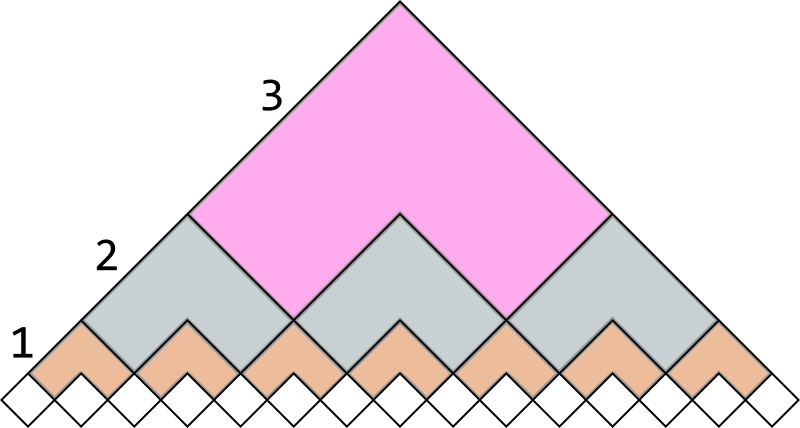
\includegraphics[width=0.7\linewidth]{part_02_Foundations/chapter_07_ClassicalParsing/figures/02_Valiant/layers.png}
  \caption{V-образные слои в модифицированном алгоритме: каждый слой состоит из непересекающихся подматриц одного размера}
  \label{fig:ValiantLayers}
\end{figure}
\mytodo{Перевести в TikZ}

\subsection{Сложность и свойства}

Асимптотическая сложность алгоритма Валианта составляет $O(|N|^2 \cdot \BMM{n} \cdot \log n)$, где $\BMM{n}$~--- количество операций, необходимое для умножения двух булевых матриц размера $n \times n$.
На сегодняшний день наилучшая известная оценка $\BMM{n} = O(n^\omega)$ с $\omega < 2{,}38$, что даёт субкубическую сложность синтаксического анализа для произвольных КС-грамматик.

Однако, как уже отмечалось, алгоритм Валианта существенно опирается на возможность топологически упорядочить обход матрицы $T$, что не обобщается на случай произвольных графов~\sidecite{Yannakakis}.
По этой причине для задач анализа графов с контекстно-свободными ограничениями (глава~\ref{chpt:CFPQ}) используются преимущественно обобщения CYK и GLR, а не алгоритма Валианта.

\mytodo{Добавить пример. Без SPPF. Вход: "a b a b a b". Грамматика: S -> eps | S S | a S b. Визуализировать с использованием FLPQ: исходная граммтика, грамматика в НФХ, матрицы. Матрицы расположить по две в ряд.}

\section{Построение множеств $\first$ и $\follow$}
\label{sec:FirstAndFollow}
\tikzsetfigurename{FirstAndFollow_}

При синтаксическом анализе для однозначного выбора применяемой продукции грамматики необходимо <<заглядывать вперёд>>~---
знать, какие терминалы могут находиться на тех или иных позициях выводимой цепочки.
Для этого используются множества $\first[k]$ и $\follow[k]$.
Идейно их можно понимать как первые или, соответственно, последующие $k$ символов в результирующем выводе при использовании нетерминала $A$.
Данную мысль хорошо иллюстрирует рисунок~\ref{fig:first_follow}.

\begin{marginfigure}
    \begin{center}
        \input{part_02_Foundations/chapter_07_ClassicalParsing/figures/03_FirstAndFollow/fig_first_follow.tex}
    \end{center}
    \caption{Схематичное изображение $\first[k](A)$ и $\follow[k](A)$}
    \label{fig:first_follow}
\end{marginfigure}

Эти множества играют ключевую роль при построении управляющих таблиц для алгоритмов синтаксического анализа:
в нисходящем анализе они определяют, какую продукцию применять (раздел~\ref{sec:TopDown}),
в восходящем~--- помогают разрешать конфликты (раздел~\ref{sec:BottomUp}).

Дадим формальные определения для произвольного $k$, а затем специализируем их для наиболее распространённого на практике случая $k = 1$.

Формально эти множества определяются следующим образом.

\begin{definition}
    \label{def:firstk}
    Пусть $G = \langle N, \Sigma, P, S \rangle$~--- КС-грамматика.
    Множество $\first[k]$ определено для сентенциальной формы $\alpha \in (N \cup \Sigma)^*$ следующим образом:
    \[
    \first[k](\alpha) = \{\, \omega \in \Sigma^* \mid \alpha \derives{} \omega \text{ и } |\omega| < k \text{ либо } \exists \beta: \alpha \derives{} \omega \beta \text{ и } |\omega| = k \,\}.
    \]
\end{definition}

Иными словами, $\first[k](\alpha)$~--- это множество всех терминальных цепочек длины не более $k$, которые могут находиться в начале (быть префиксом) любой цепочки, выводимой из $\alpha$.

\begin{definition}
    \label{def:followk}
    Пусть $G = \langle N, \Sigma, P, S \rangle$~--- КС-грамматика.
    Множество $\follow[k]$ определено для сентенциальной формы $\beta \in (N \cup \Sigma)^*$ следующим образом:
    \[
    \follow[k](\beta) = \{\, \omega \in \Sigma^* \mid \exists \gamma, \alpha: S \derives{} \gamma \beta \alpha \text{ и } \omega \in \first[k](\alpha) \,\}.
    \]
\end{definition}

Иными словами, $\follow[k](\beta)$~--- это множество всех терминальных цепочек длины не более $k$, которые могут следовать непосредственно за $\beta$ в некоторой сентенциальной форме, выводимой из аксиомы.

Приведённые выше определения носят общий характер.
Однако на практике подавляющее большинство алгоритмов синтаксического анализа ограничивается одним символом предпросмотра, поэтому далее мы специализируем их для $k = 1$ и подробно рассмотрим построение множеств именно в этом случае.

На практике наиболее распространён случай $k = 1$.
Для него определения упрощаются:

\[
\first(\alpha) = \{\, a \in \Sigma \mid \exists \gamma \in (N \cup \Sigma)^*: \alpha \derives{} a \gamma \,\}, \quad \alpha \in (N \cup \Sigma)^*.
\]

Иными словами, $\first(\alpha)$~--- множество терминалов, с которых может начинаться цепочка, выводимая из $\alpha$, а также $\varepsilon$, если $\alpha \derives{} \varepsilon$.

\[
\follow(\beta) = \{\, a \in \Sigma \mid \exists \gamma, \alpha \in (N \cup \Sigma)^* : S \derives{} \gamma \beta a \alpha \,\}, \quad \beta \in (N \cup \Sigma)^*.
\]

Иными словами, $\follow(\beta)$~--- множество терминалов, которые могут следовать непосредственно за $\beta$ в некоторой сентенциальной форме, выводимой из аксиомы.

Теперь перейдём непосредственно к алгоритмам вычисления этих множеств и начнём с $\first$.

Множество $\first$ для произвольной сентенциальной формы можно вычислить, пользуясь следующими соотношениями.
\begin{itemize}
    \item $\first(a \alpha) = \{a\}$, где $a \in \Sigma$, $\alpha \in (N \cup \Sigma)^*$;
    \item $\first(\varepsilon) = \{\varepsilon\}$;
    \item $\first(\alpha \beta) = \first(\alpha) \cup (\first(\beta) \text{, если } \varepsilon \in \first(\alpha))$;
    \item $\first(A) = \first(\alpha) \cup \first(\beta)$, если в грамматике есть правила $A \to \alpha \mid \beta$, для нетерминала $A \in N$.
\end{itemize}

Поскольку определения взаимно рекурсивны (в правую часть могут входить нетерминалы, для которых $\first$ ещё не вычислен), на практике эти соотношения применяются итеративно до достижения неподвижной точки.

Зная $\first$ для всех нетерминалов, можно вычислить и $\follow$.

Алгоритм для вычисления множества $\follow$ для нетерминалов грамматики состоит из следующих шагов.
\begin{enumerate}
    \item Инициализация: $\follow(X) = \varnothing$ для всех $X \in N$.
    \item Добавляем маркер конца строки в множество $\follow$ аксиомы:
    \[
    \follow(S) = \follow(S) \cup \{\$\}, \quad \text{где } S~\text{--- стартовый нетерминал}.
    \]
    \item Для всех правил вида $A \to \alpha X \beta$:
    \[
    \follow(X) = \follow(X) \cup (\first(\beta) \setminus \{\varepsilon\}).
    \]
    \item Для всех правил вида $A \to \alpha X$ и $A \to \alpha X \beta$, где $\varepsilon \in \first(\beta)$:
    \[
    \follow(X) = \follow(X) \cup \follow(A).
    \]
    \item Шаги 3 и 4 повторяются, пока в строящиеся множества добавляются новые элементы.
\end{enumerate}

Проиллюстрируем работу обоих алгоритмов на примере.

\begin{example}
\label{ex:first_follow}
Рассмотрим грамматику $G$ со следующими продукциями:
\begin{align*}
    S  &\to a S'                     & A' &\to b \mid a \\
    S' &\to A b B S' \mid \varepsilon & B  &\to c \mid \varepsilon \\
    A  &\to a A' \mid \varepsilon
\end{align*}

Вычислим множества $\first$ для нетерминалов грамматики $G$:
\begin{align*}
    \first(S)  &= \{ a \}           & \first(B)  &= \{ c, \varepsilon \} \\
    \first(A)  &= \{ a, \varepsilon \} & \first(S') &= \{ a, b, \varepsilon \} \\
    \first(A') &= \{ a, b \}
\end{align*}

Вычислим множества $\follow$ для нетерминалов грамматики $G$:
\begin{align*}
    \follow(S)  &= \{ \$ \}                                &                                               \\
    \follow(S') &= \{ \$ \}                                &\qquad (S \to a S')                            \\
    \follow(A)  &= \{ b \}                                 &\qquad (S' \to A b B S')                       \\
    \follow(A') &= \{ b \}                                 &\qquad (A \to a A')                            \\
    \follow(B)  &= \{ a, b, \$ \}                          &\qquad (S' \to A b B S',\, \varepsilon \in \first(S'))
\end{align*}

В комментариях справа указаны правила грамматики, из которых были получены соответствующие элементы множеств $\follow$.
\end{example}

\section{Нисходящий синтаксический анализ}
\label{sec:TopDown}
\tikzsetfigurename{TopDown_}

\subsection{Рекурсивный спуск}

Идея рекурсивного спуска основана на использовании программного стека вызовов в качестве стека магазинного автомата. Достигается это следующим образом.
\begin{itemize}
  \item Для каждого нетерминала создаётся функция, принимающая ещё не обработанный остаток строки и возвращающая пару: результат вывода префикса данной строки из соответствующего нетерминала и не обработанный остаток строки. В случае распознавателя результат вывода~--- логическое значение (выводится/не выводится).
  \item Каждая такая функция реализовывает обработку цепочки согласно правым частям правил для соответствующих нетерминалов: считывание символа входа при обработке терминального символа, вызов соответствующей функции при обработке нетерминального.
\end{itemize}

У такого подхода есть два ограничения:
\begin{enumerate}
  \item Не работает с леворекурсивными грамматиками, то есть грамматиками, вывод в которых может принимать следующий вид:
  \[
  S \to \cdots \to \underline{N_i} \alpha \to \cdots \underline{N_i} \beta \to \cdots \omega
  \]
  \item Шаги должны быть однозначными.
\end{enumerate}

\begin{example}

Построим функцию рекурсивного спуска для продукции $S \rightarrow aSbS \mid \varepsilon$.

\begin{algorithm}
  \floatname{algorithm}{Listing}
%\begin{algorithmic}[1]
%\caption{Функция рекурсивного спуска}
%\Function{S}{$\omega$}
%    \If {(len$(\omega)=0$)}
%    \Comment{{\footnotesize Пустая цепочка выводима из $S$}}
%    \State{\Return \textit{(true, $\omega$)}}
%    \EndIf

%    \If{$(\omega = a :: tl)$}
%        \Comment{{\footnotesize Выводимая из $S$ подстрока должна начинаться с $a$}}
%        \State{$res,tl' = $ S($tl$)}
%        \Comment{{\footnotesize Затем должна идти подстрока, выводимая из $S$}}
%        \If{res \&\&  $tl' = b :: tl''$}
%           \Comment{{\footnotesize Если вызов закончился успешно, то надо проверить, что следующий символ --- это $b$}}
%           \State{\Return $S(tl'')$}
%           \Comment{{\footnotesize И снова попробовать вывести перфикс из $S$}}
%         \Else
%           \State{\Return \textit{(false, $tl'$)}}
%        \EndIf
%    \Else
%        \State{\Return \textit{(false, $\omega$)}}
%    \EndIf
%\EndFunction

%\end{algorithmic}
\end{algorithm}
\end{example}

Если возвращаемое значение этой функции~--- пара вида \textit{(true, [])}, то разбор завершился успехом.

Данный подход применяется как для ручного написания синтаксических нализаторов, так и при генерации анализаторов по грамматике.

\subsection{LL(k)-алгоритм синтаксического анализа}

LL(k)~--- алгоритм синтаксического анализа~--- нисходящий анализ без отката, но с предпросмотром.
Решение о том, какую продукцию применять, принимается на основании k следующих за текущим символом.
Временная сложность алгоритма $O(n)$, где $n$~--- длина слова.

Алгоритм использует входной буфер, стек для хранения промежуточных данных и таблицу анализатора, которая управляет процессом разбора.
В ячейке таблицы указано правило, которое нужно применять, если рассматривается нетерминал $A$, а следующие $m$ символов строки~--- $t_{1} \dots t_{m}$, где $m \leq k$.
Также в таблице выделена отдельная колонка для $\$$~--- маркера конца строки.

\begin{center}
  \begin{tabular}{ c || c | c | c | c }
             & $\dots$ & $t_{1} \dots t_{m}$ & $\dots$ & $\$$ \\ \hline
    $\dots$  & $\dots$ & $\dots$ & $\dots$ & $\dots$ \\ \hline
    $A$  & $\dots$ & $A \to \alpha$ & $\dots$ & $\dots$ \\ \hline
    $\dots$  & $\dots$ & $\dots$ & $\dots$ & $\dots$
  \end{tabular}
\end{center}

Для построения таблицы вычисляются множества $\first[k]$ и $\follow[k]$, определение и алгоритмы вычисления которых подробно разобраны в разделе~\ref{sec:FirstAndFollow}.
Пример вычисления для конкретной грамматики приведён в примере~\ref{exmpl:first_follow}.

Управляющая таблица LL(k) анализатора заполняется следующим образом: продукции $A \to \alpha, \alpha \neq \varepsilon$ помещаются в ячейки $(A, a)$, где $a \in \first(\alpha)$, продукции $A \to \alpha$~--- в ячейки $(A, a)$, где $a \in \follow(A)$, если $\varepsilon \in \first(\alpha)$

\begin{example}

Пример таблицы для грамматики $S \to aSbS \mid \varepsilon$

\begin{center}
\begin{tabular}{ r || c | c || c | c | c }
N & $\first$ & $\follow$ & a & b & $\$ $ \\ \hline
$S$ & $\{ a, \varepsilon \}$ & $\{ b, \$ \}$ & $S \rightarrow aSbS$ & $S \rightarrow \varepsilon$ & $S \rightarrow \varepsilon$
\end{tabular}
\end{center}

\end{example}

Однако, не для всех грамматик по множествам $\first[k]$ и $\follow[k]$ возможно выбрать применяемую продукцию, а значит, нельзя однозначно построить таблицу, необходимую для работы алгоритма, поэтому данный алгоритм применим только для грамматик особого класса~--- LL(k).

\begin{definition}
  LL(k) грамматика~--- грамматика, для которой на основании множеств $\first[k]$ и $\follow[k]$ можно однозначно определить, какую продукцию применять.
\end{definition}

Важно заметить, что при больших $k$ управляющая таблица сильно разрастается, поэтому на практике данный алгоритм применим для небольших значений $k$.

Интерпретатор автомата принимает входную строку и построенную управляющую таблицу и работает следующим образом.
В каждый момент времени конфигурация автомата это позиция во входной строке и стек.
В начальный момент времени стек пуст, а позиция во входной строке соответствует её началу.
На первом шаге в стек добавляются последовательно сперва символ конца строки, затем стартовый нетерминал.
На каждом шаге анализируется существующая конфигурация и совершается одно из действий.
\begin{itemize}
\item Если текущая позиция~--- конец строки и вершина стека~--- символ конца строки, то успешно завершаем разбор.
\item Если текущая вершина стека~--- терминал, то проверяем, что позиция в строке соответствует этому терминалу. Если да, то снимаем элемент со стека, сдвигаем позицию на единицу и продолжаем разбор. Иначе завершаем разбор с ошибкой.
\item Если текущая вершина стека~--- нетерминал $N_i$ и текущий входной символ $t_j$, то ищем в управляющей таблице ячейку с координатами $(N_i, t_j)$ и записываем на стек содержимое этой ячейки.
\end{itemize}

\begin{example}Пример работы LL анализатора.
Рассмотрим грамматику $S \to aSbS \mid \varepsilon$ и выводимое слово $\omega = abab$.

Рассмотрим пошагово работу алгоритма c построением дерева, будем использовать таблицу, построенную в предыдущем примере:

\begin{enumerate}
  \item Начало работы.

  Стек: \,
    \begin{tabular}[c]{ |c| }
        \\ \hline
        \$ \\ \hline
    \end{tabular}
    \qquad  \qquad \qquad  \qquad входное слово: \,
    \begin{tabular}[c]{ |c|c|c|c|c| }
        \hline
        \textcolor{red}{a} & b & a & b & \$ \\ \hline
    \end{tabular}

Финальный символ лежит на стеке, а указатель указывает на первый символ слова.

  \item кладем стартовый символ на стек

    Стек: \,
    \begin{tabular}[c]{ |c| }
        \\ \hline
        $S$ \\ \hline
        \$ \\ \hline
    \end{tabular}
    \qquad  \qquad \qquad  \qquad входное слово: \,
    \begin{tabular}[c]{ |c|c|c|c|c| }
        \hline
        \textcolor{red}{a} & b & a & b & \$ \\ \hline
    \end{tabular}

  \item Ищем ячейку с координатами (S, a), применяем продукцию из ячейки.

    Стек: \,
    \begin{tabular}[c]{ |c| }
        \\ \hline
        $a$ \\ \hline
        $S$ \\ \hline
        $b$ \\ \hline
        $S$ \\ \hline
        \$ \\ \hline
    \end{tabular}
    \qquad  \qquad \qquad  \qquad входное слово: \,
    \begin{tabular}[c]{ |c|c|c|c|c| }
        \hline
        \textcolor{red}{a} & b & a & b & \$ \\ \hline
    \end{tabular}

    \begin{center}
      \resizebox{1cm}{1cm}{
    \input{part_02_Foundations/chapter_07_ClassicalParsing/figures/04_TopDown/04_TopDown_fig_02.tex}
    }
  \end{center}

\item Снимаем терминал $a$ со стека и двигаем указатель.

    Стек: \,
    \begin{tabular}[c]{ |c| }
        \\ \hline
        $S$ \\ \hline
        $b$ \\ \hline
        $S$ \\ \hline
        \$ \\ \hline
    \end{tabular}
    \qquad  \qquad \qquad  \qquad входное слово: \,
    \begin{tabular}[c]{ |c|c|c|c|c| }
        \hline
        a & \textcolor{red}{b} & a & b & \$ \\ \hline
    \end{tabular}

    \begin{center}
      \resizebox{1.5cm}{1.3cm}{
    \input{part_02_Foundations/chapter_07_ClassicalParsing/figures/04_TopDown/04_TopDown_fig_03.tex}
    }
  \end{center}

\item Ищем ячейку с координатами (S, b), применяем продукцию из ячейки.

    Стек: \,
    \begin{tabular}[c]{ |c| }
        \\ \hline
        $b$ \\ \hline
        $S$ \\ \hline
        \$ \\ \hline
    \end{tabular}
    \qquad  \qquad \qquad  \qquad входное слово: \,
    \begin{tabular}[c]{ |c|c|c|c|c| }
        \hline
        a & \textcolor{red}{b} & a & b & \$ \\ \hline
    \end{tabular}

    \begin{center}
      \resizebox{3cm}{2cm}{
    \input{part_02_Foundations/chapter_07_ClassicalParsing/figures/04_TopDown/04_TopDown_fig_04.tex}
  }
\end{center}

\item Снимаем терминал $b$ со стека и двигаем указатель.

    Стек: \,
    \begin{tabular}[c]{ |c| }
        \\ \hline
        $S$ \\ \hline
        \$ \\ \hline
    \end{tabular}
    \qquad  \qquad \qquad  \qquad входное слово: \,
    \begin{tabular}[c]{ |c|c|c|c|c| }
        \hline
        a & b & \textcolor{red}{a} & b & \$ \\ \hline
    \end{tabular}

    \begin{center}
      \resizebox{3cm}{2cm}{
    \input{part_02_Foundations/chapter_07_ClassicalParsing/figures/04_TopDown/04_TopDown_fig_05.tex}
  }
\end{center}

  \item Ищем ячейку с координатами (S, a), применяем продукцию из ячейки.

    Стек: \,
    \begin{tabular}[c]{ |c| }
        \\ \hline
        $a$ \\ \hline
        $S$ \\ \hline
        $b$ \\ \hline
        $S$ \\ \hline
        \$ \\ \hline
    \end{tabular}
    \qquad  \qquad \qquad  \qquad входное слово: \,
    \begin{tabular}[c]{ |c|c|c|c|c| }
        \hline
        a & b & \textcolor{red}{a} & b & \$ \\ \hline
    \end{tabular}

    \begin{center}
      \resizebox{5cm}{3cm}{
    \input{part_02_Foundations/chapter_07_ClassicalParsing/figures/04_TopDown/04_TopDown_fig_06.tex}
    }
  \end{center}

\item Снимаем терминал $a$ со стека и двигаем указатель.

    Стек: \,
    \begin{tabular}[c]{ |c| }
        \\ \hline
        $S$ \\ \hline
        $b$ \\ \hline
        $S$ \\ \hline
        \$ \\ \hline
    \end{tabular}
    \qquad  \qquad \qquad  \qquad входное слово: \,
    \begin{tabular}[c]{ |c|c|c|c|c| }
        \hline
        a & b & a & \textcolor{red}{b} & \$ \\ \hline
    \end{tabular}

    \begin{center}
      \resizebox{6cm}{3.5cm}{
    \input{part_02_Foundations/chapter_07_ClassicalParsing/figures/04_TopDown/04_TopDown_fig_07.tex}
    }
  \end{center}

\item Ищем ячейку с координатами (S, b), применяем продукцию из ячейки.

    Стек: \,
    \begin{tabular}[c]{ |c| }
        \\ \hline
        $b$ \\ \hline
        $S$ \\ \hline
        \$ \\ \hline
    \end{tabular}
    \qquad  \qquad \qquad  \qquad входное слово: \,
    \begin{tabular}[c]{ |c|c|c|c|c| }
        \hline
        a & b & a & \textcolor{red}{b} & \$ \\ \hline
    \end{tabular}

    \begin{center}
      \resizebox{6cm}{3.5cm}{
    \input{part_02_Foundations/chapter_07_ClassicalParsing/figures/04_TopDown/04_TopDown_fig_08.tex}
    }
  \end{center}

\item Снимаем терминал $b$ со стека и двигаем указатель.

    Стек: \,
    \begin{tabular}[c]{ |c| }
        \\ \hline
        $S$ \\ \hline
        \$ \\ \hline
    \end{tabular}
    \qquad  \qquad \qquad  \qquad входное слово: \,
    \begin{tabular}[c]{ |c|c|c|c|c| }
        \hline
        a & b & a & b & \textcolor{red}{\$} \\ \hline
    \end{tabular}

    \begin{center}
      \resizebox{6cm}{3.5cm}{
      \input{part_02_Foundations/chapter_07_ClassicalParsing/figures/04_TopDown/04_TopDown_fig_09.tex}
    }
  \end{center}

\item Ищем ячейку с координатами (S, \$), применяем продукцию из ячейки.

    Стек: \,
    \begin{tabular}[c]{ |c| }
        \\ \hline
        \$ \\ \hline
    \end{tabular}
    \qquad  \qquad \qquad  \qquad входное слово: \,
    \begin{tabular}[c]{ |c|c|c|c|c| }
        \hline
        a & b & a & b & \textcolor{red}{\$} \\ \hline
    \end{tabular}

    \begin{center}
      \resizebox{6cm}{3.5cm}{
      \input{part_02_Foundations/chapter_07_ClassicalParsing/figures/04_TopDown/04_TopDown_fig_10.tex}
    }
  \end{center}

\item Оказались в конце строки и на вершине стека символ конца~--- завершаем разбор.

\end{enumerate}

\end{example}

Дерево строится сверху вниз, от корня к листьям. Для этого выолняются следующие шаги алгоритма:
\begin{itemize}
  \item В ситуации, когда мы читаем очередной терминал (на вершине стека и во входе одинаковые терминалы), мы создаём лист с соответствующим терминалом.
  \item В ситуации, когда мы заменяем нетерминал на стеке на правую часть продукции в соответствии с управляющей таблицей, мы создаём нетерминальный узел соответствующий применяемой продукции.
\end{itemize}

Данное семейство алгоритмов всё так же не работает с леворекурсивными грамматиками и с неоднозначными грамматиками.

Таким образом, по некоторым грамматикам можно построить LL(k) анализатор (назовём их LL(k) грамматиками), но не по всем.
С левой рекурсией, конечно, можно бороться, так как существуют алгоритмы устранения левой и скрытой левой рекурсии, а вот с неоднозначностями ничего не поделаешь.


\subsection{Обобщённый нисходящий анализ}

Можно построить анализатор, работающий с произвольными КС-грамматиками.
Generalized LL (GLL)~\cite{Scott:2010:GP:1860132.1860320,10.1007/978-3-662-46663-6_5}

Обзор:~\cite{Cappers2014ExploringAV}, история и т.д.~\cite{Afroozeh2019PracticalGT}

Принцип работы остается абсолютно таким же, как для табличного LL:
\begin{itemize}
  \item Сначала по грамматике строится \textit{управляющая} таблица
  \item Затем построенная таблица команд и непосредственно анализируемое слово поступают на вход абстрактному интерпретатору.
  \item Для своей работы интерпретатор поддерживает некоторую вспомогательную структуру данных (стек для LL).
  \item Один шаг разбора состоит в том, чтобы рассмотреть текущую позицию в слове, применить все соответствующие ей правила из таблицы и при возможности сдвинуть позицию разбора вправо.
\end{itemize}

Где в этой схеме возникают ограничения на вид обрабатываемой грамматики для алгоритма LL? На самом первом шаге~--- при построении таблицы может возникнуть ситуация, когда одному нетерминалу $N_j$ и последовательности $first_k(N_j)$ соответствует несколько продукций грамматики. В этом случае грамматика признавалась не соответствующей классу LL(k) и отвергалась анализатором.

Теперь же мы разрешим такую ситуацию и в этом случае в ячейку таблицы будем записывать все продукции грамматики, соответствующие этой ячейке. Однако сразу же возникает вопрос~--- а что делать интерпретатору, когда при разборе ему необходимо применить правило, состоящее из нескольких продукций? Общий ответ такой~--- необходим некоторый вид недетерминизма, при котором интерпретатор мог бы <<параллельно>> обрабатывать несколько возможных вариантов синтаксического разбора.

Эти два свойства (модифицированная управляющая таблица и недетерминизм) суть главные принципиальные отличия GLL(k) от LL(k). Далее мы перейдем к рассмотрению непосредственно технической реализации описанного алгоритма.

Нам необходимо научиться задавать различные ветви (пути) синтаксического разбора и переключаться между ними. Заметим, что состояние любой ветви в любой момент времени суть следующее: необходимо распознать символ $N_j \in N \cup \Sigma$ из продукции $X$, начиная с элемента слова под индексом $i$. Т.е. имеем позицию в слове и позицию символа в продукции. Последнее принято называть \textit{слотом грамматики}.

\begin{definition}
  Пусть $G = \langle N, \Sigma, P, S \rangle$~--- КС-грамматика. \textit{Слотом грамматики} $G$ (позицией грамматики $G$) назовем пару из продукции $X \in P$ и позиции $0 \leq q \leq length(body(X))$ тела продукции $X$. При этом введем следующее обозначение $X ::= \alpha \cdot \beta, \quad \alpha,\beta \in (N \cup \Sigma)^*$, где $ \cdot $ указывает на позицию в продукции.
\end{definition}

Описанная пара позиций уже однозначно задает состояние синтаксического разбора. Имеем множество состояний и переходов между ними~--- возникает естественное желание воспользоваться терминами графов для представления этой структуры. Такую конструкцию называют \textit{граф-структурированный стек} или \textit{GSS} (Graph Structured Stack), который впервые был предложен Масару Томитой ~\cite{tomita1988graph} в контексте восходящего анализа. GSS будет являться рабочей структурой нашего нового интерпретатора вместо стека для LL. Состояние разбора вместе с узлом GSS мы будет называть \textit{дескриптором}.

\begin{definition}
  Пусть $G = \langle N, \Sigma, P, S \rangle$~--- КС-грамматика, $X$~--- слот грамматики $G$, $i$~--- позиция в слове $ w $ над алфавитом $\Sigma$, а $ u $~--- узел GSS. \textit{Дескриптором} назовём тройку $ (X, u, i) $.
\end{definition}

Есть несколько способов задания GSS для алгоритма GLL. Вариант, предложенный самими авторами алгоритма, оперирует непосредственно парами из позиции слова и слота грамматики в качестве состояний (и узлов графа). Такой метод является довольно простым и наглядным, но, как описано в работе~\cite{10.1007/978-3-662-46663-6_5}, не самым эффективным. Предложим сразу чуть более оптимальное представление: заметим, что шаги разбора, соответствующие одному и тому же нетерминалу и позиции слова, должны выдавать один и тот же результат независимо от конкретной продукции грамматики, в которой стоит этот нетерминал. Поэтому заводить по узлу на каждый слот грамматики довольно избыточно~--- вместо этого в качестве состояния будем использовать пары из нетерминала и позиции слова, а позиции грамматики будем записывать на рёбрах.

Итак, мы научились задавать состояния с помощью дескрипторов, а также определились со вспомогательной структурой GSS. Теперь можно перейти к рассмотрению непосредственно самого алгоритма, суть которого довольно проста и напоминает BFS по неявному графу.

Дескриптор задает состояние, которое необходимо обработать. При этом мы без какой-либо дополнительной информации можем продолжить анализ входа из состояния, задаваемого этим дескриптором. В процессе обработки мы можем получить несколько новых состояний. Поэтому будем поддерживать множество $ R $ дескрипторов на обработку~--- на каждом шаге извлекаем один из множества, проводим анализ и добавляем во множество новые полученные.

При каких условиях этот процесс будет конечен? Ну, например, если мы каждое состояние будем обрабатывать не более одного раза. И действительно, поскольку наш интерпретатор является <<чистым>> в том смысле, что для одного и того же состояния каждый раз будут получены одинаковые результаты, проводить анализ дважды не имеет смысла. Поэтому будем также поддерживать множество $ U $ всех полученных в ходе разбора дескрипторов, и добавлять в $ R $ только те, которых еще нет в $ U $.

И наконец, заключительная и самая главная часть~--- как происходит обработка дескриптора?
Пусть дескриптор имеет вид $ (X, u, i) $, а входное слово обозначим $ W $. Есть три возможных варианта, в зависимости от вида позиции грамматики $ X $~--- разберем каждый из них по отдельности;

\begin{itemize}
  \item $ X ::= \alpha \cdot t \beta $, т.е. указатель смотрит на терминал~--- в этом случае новых дескрипторов добавлено не будет. Если $ W[i] = t $, то мы сдвигаем указатель слота, переходя к рассмотрению $ X ::= \alpha t \cdot \beta $, и инкрементируем позицию $ i $ в слове. В противном же случае сразу переходим к следующему дескриптору, таким образом терминируя текущую ветвь разбора.

  \item $ X ::= \alpha \cdot A \beta $, т.е. указатель смотрит на нетерминал. Нам нужен GSS узел $ v $ вида $ (A, i) $ и ребро $ (u, X ::= \alpha A \cdot \beta, v) $ (ребро из $ u $ в $ v $ с пометкой $ X ::= \alpha A \cdot \beta $). Если такой узел и ребро уже существуют в нашем GSS, берем их, иначе~--- создаём. Далее в $ R $ добавляем по дескриптору для узла $ v $ и каждого правила грамматики из ячейки управляющей таблицы для нетерминала $ A $ (конечно, если их еще не было в $ U $). На этом обработка текущего дескриптора завершается.

  \item $ X ::= \alpha \cdot $, т.е. указатель находится в конце продукции. Продукция разобрана, а значит, интерпретатору необходимо вернуться из разбора $ X $ к вызывающему правилу и продолжить разбор там (это, в некотором смысле, соответствует возврату из функции разбора нетерминала в методе рекурсивного спуска). По каждому исходящему ребру $ (u, Y, v) $ добавляем (если уже не существует) дескриптор $(Y, v, i)$.
\end{itemize}

Результатом синтаксического разбора является успех тогда и только тогда, когда был достигнут дескриптор вида $ (S ::= \alpha \cdot, s, n) $, где слот грамматики представляет собой любое правило для аксиомы $ S $, узел GSS $ s $ состоит из аксиомы $ S $ и 0, а позиция входного слова равна его длине $ n $. Если же после разбора всех полученных дескрипторов указанный найден не был, результатом будет являться провал.

Давайте посмотрим, как такой алгоритм справится с неоднозачной грамматикой с леворекурсивным правилом.

\begin{example}
  \label{exmpl:GLLExample1}
  Пусть грамматика $ G $ имеет вид $ S \to SSS \mid SS \mid a $, а разбираемое слово $ w = aaa $. Тогда GSS, соответствующий разбору $S \Rightarrow SSS \Rightarrow aSS \Rightarrow aaS \Rightarrow aaa$, будет выглядеть следующим образом (для удобства каждое ребро дополнительно пронумеровано):

  \begin{center}
    \input{part_02_Foundations/chapter_07_ClassicalParsing/figures/04_TopDown/complete}
  \end{center}

  Далее мы пошагово рассмотрим процесс его построения, а пока отметим несколько особенностей:

  \begin{itemize}
    \item Это \textit{неполный} GSS. Для задачи синтаксического анализа такого достаточно, поскольку если в какой-то момент был достигнут финальный дескриптор, то обрабатывать все последующие уже не нужно. Однако, для задачи построения SPPF, как мы отметим далее, это уже не так, поскольку она требует агрегирования всех возможных путей разбора.

    \item Обратите особое внимание на наличие петель. Они как раз-таки и обеспечивают эффективную работу с леворекурсивными правилами, поскольку переиспользуются уже существующие узлы. При этом кратных петель, понятно, не создается, т.к. мы запоминаем все достигнутые дескрипторы в множестве $ U $ и дублирующих дескрипторов в рабочее множество $ R $ не добавляем.

    \item В GSS не создаются узлы, соответствующие разбору терминалов (например, $a, 0$). В действительности так можно было бы сделать. Но тогда при обработке слота, указывающего на терминал, сначала бы создался узел GSS, затем интерпретатор сверил бы терминал и символ в слове, после чего, если они совпали, произошел бы возврат из узла, а если нет, узел был бы отброшен и интерпретатор перешел бы к другому дескриптору. Таким образом, при любом случае сначала создается узел, затем выполняется проверка, после чего узел сразу отбрасывается. Для того, чтобы не создавать такие <<одноразовые>> узлы, проверка терминалов выполняется in-place.
  \end{itemize}

  Пронумеруем продукции и выпишем управляющую таблицу:

  \begin{table}[!htb]
    \begin{minipage}{.5\linewidth}
      \centering
      \begin{tabular}{lc}
        $S \to S S S$ & (0) \\
        $S \to S S$   & (1) \\
        $S \to a$     & (2)
      \end{tabular}
    \end{minipage}%
    \begin{minipage}{.5\linewidth}
      \centering
      \begin{tabular}{ r || c || c | c}
        N   & $\first$  & a     & $\$ $ \\ \hline
        $S$ & $\{ a \}$ & 0,1,2 &
      \end{tabular}
    \end{minipage}
  \end{table}

  Разумеется, что конкретный порядок исполнения алгоритма будет зависеть, например, от используемой в качестве рабочего множества $ R $ структуры данных и от порядка обработки правил из ячейки управляющей таблицы. Рассмотрим лишь один из возможных вариантов:

  \begin{enumerate}
    \item Для начала мы создаем узел GSS $ s_0 = (S, 0) $ и дескрипторы для правил из ячейки таблицы $ S, a $: $ (S \to \cdot SSS, s_0, 0), (S \to \cdot SS, s_0, 0), (S \to \cdot a, s_0, 0) $.

    \begin{center}
      \input{part_02_Foundations/chapter_07_ClassicalParsing/figures/04_TopDown/state0}
    \end{center}

    \item При обработке $ (S \to \cdot S S S, s_0, 0) $ образовываются петля 1 и дескрипторы \linebreak $ (S \to \cdot SSS, s_0, 0), (S \to \cdot SS, s_0, 0), (S \to \cdot a, s_0, 0) $, которые уже содержатся в множестве $ U $ после шага 1 и поэтому не добавляются повторно.

    \begin{center}
      \input{part_02_Foundations/chapter_07_ClassicalParsing/figures/04_TopDown/state1}
    \end{center}

    \item При обработке $ (S \to \cdot S S, s_0, 0) $ образовывается петля 2, а в остальном аналогично \mbox{шагу 2.}

    \begin{center}
      \input{part_02_Foundations/chapter_07_ClassicalParsing/figures/04_TopDown/state2}
    \end{center}

    \item При обработке $ (S \to \cdot a, s_0, 0) $ мы распознаем терминал $a$ на позиции 0 и, возвращаясь по петлям 1 и 2, добавляем дескрипторы $ (S \to S \cdot S S, s_0, 1), (S \to S \cdot S, s_0, 1) $.

    \item При обработке $ (S \to S \cdot S S, s_0, 1) $ образовываем узел $s_1 = (S, 1)$ с исходящим ребром 3 и добавляем дескрипторы $ (S \to \cdot SSS, s_1, 1), (S \to \cdot SS, s_1, 1), (S \to \cdot a, s_1, 1) $.

    \begin{center}
      \input{part_02_Foundations/chapter_07_ClassicalParsing/figures/04_TopDown/state3}
    \end{center}

    \item При обработке $ (S \to S \cdot S, s_0, 1) $ образовываем ребро 4, новых дескрипторов не добавляется.

    \begin{center}
      \input{part_02_Foundations/chapter_07_ClassicalParsing/figures/04_TopDown/state4}
    \end{center}

    \item Обработка дескриптора $ (S \to \cdot S S S, s_1, 1) $ аналогична шагу 2 с добавлением петли 5.

    \begin{center}
      \input{part_02_Foundations/chapter_07_ClassicalParsing/figures/04_TopDown/state5}
    \end{center}

    \item Обработка дескриптора $ (S \to \cdot S S, s_1, 1) $ аналогична шагу 3 с добавлением петли 6.

    \begin{center}
      \input{part_02_Foundations/chapter_07_ClassicalParsing/figures/04_TopDown/state6}
    \end{center}

    \item При обработке $ (S \to \cdot a, s_1, 1) $ мы распознаем терминал $a$ на позиции 1 и, возвращаясь по ребрам 3 и 4, добавляем дескрипторы $ (S \to S S \cdot S, s_0, 2), (S \to S S \cdot, s_0, 2) $, а также, возвращаясь по петлям 5 и 6, добавляем дескрипторы $ (S \to S \cdot S S, s_1, 2), (S \to S \cdot S, s_1, 2) $.

    \item При обработке $ (S \to S S \cdot S, s_0, 2) $ образовываем узел $s_2 = (S, 2)$ с исходящим ребром 7 и добавляем дескрипторы $ (S \to \cdot SSS, s_2, 2), (S \to \cdot SS, s_2, 2), (S \to \cdot a, s_2, 2) $.

    \begin{center}
      \input{part_02_Foundations/chapter_07_ClassicalParsing/figures/04_TopDown/state7}
    \end{center}

    \item Обработка дескриптора $ (S \to \cdot S S S, s_2, 2) $ аналогична шагу 2 с добавлением петли 8.

    \begin{center}
      \input{part_02_Foundations/chapter_07_ClassicalParsing/figures/04_TopDown/state8}
    \end{center}

    \item Обработка дескриптора $ (S \to \cdot S S, s_2, 2) $ аналогична шагу 3 с добавлением петли 9.

    \begin{center}
      \input{part_02_Foundations/chapter_07_ClassicalParsing/figures/04_TopDown/complete}
    \end{center}

    \item При обработке $ (S \to \cdot a, s_2, 2) $ мы распознаем терминал $a$ на позиции 2 и, возвращаясь по ребру 7, добавляем дескриптор $ (S \to S S S \cdot, s_0, 3) $, а также, возвращаясь по петлям 8 и 9, добавляем дескрипторы $ (S \to S \cdot S S, s_2, 3), (S \to S \cdot S, s_2, 3) $.

    \item Мы достигли финального дескриптора $ (S \to S S S \cdot, s_0, 3) $, синтаксический разбор успешен.
  \end{enumerate}

\end{example}

Внимательный читатель мог заметить, что если бы в этом примере шаг 4 был выполнен перед шагом 2, разбор довольно быстро бы завершился неудачей. Отсюда вытекает следующее наблюдение: если в какой-то момент из существующего узла появилось новое ребро, необходимо пересчитать все входящие в него пути.

Для построения SPPF требуется внести лишь несколько небольших добавлений:

\begin{enumerate}
  \item В дескриптор необходимо добавить узел SPPF $ w $, который будет представлять уже разобранный префикс.
  \item Необходимо поддерживать множество $ P $ из элементов вида $ (u, z) $, где $ u $ это узел GSS, а $ z $ соответствующий ему узел SPPF, для того, чтобы переиспользовать результаты разбора, ассоциированные с узлами GSS.
  \item При обработке терминала $ t $ на позиции $ i $ ищется узел вида $ (t, i, i + 1) $, либо создается, если такого еще нет.
  \item При обработке нетерминала с помощью $ P $ ищется или при необходимости создается промежуточный узел вида $ (X, l, r) $, где $ X $ соответствующий слот грамматики, а $ l $ и $ r $ узлы SPPF, отвечающие за разбор левой и правой частей слота соответственно.
\end{enumerate}

Конкретные шаги построения SPPF будут зависеть от выбранного для него формата. Описание эффективного бинаризованного SPPF и детали его построения при выполнении GLL представлены в работе~\cite{10.1007/978-3-662-46663-6_5}.

\section{Восходящий синтаксический анализ}
\label{sec:BottomUp}
\tikzsetfigurename{BottomUp_}

Существует большое семейство LR(k) алгоритмов~--- алгоритм восходящего синтаксического анализа.
Основная идея, лежащая в основе семейства, заключается в следующем: входная последовательность символов считывается слева направо с попутным добавлением в стек и выполнением сворачивания на стеке~--- замены последовательности терминалов и нетерминалов, лежащих наверху стека, на нетерминал, если существует соответствующее правило в исходной грамматике.

Как и в случае с LL, используется магазинный автомат, управляемый таблицами, построенными по грамматике.
При этом, у LR анализатора есть два типа команд:
\begin{enumerate}
	\item shift~--- прочитать следующий символ входной последовательности, положив его в стек, и перейти в следующее состояние;
	\item reduce(k)~--- применить k-ое правило грамматики, правая часть которого уже лежит на стеке: снимаем со стека правую часть продукции и кладём левую часть.
\end{enumerate}

А управляющая таблица выглядит следующим образом.

\begin{center}
  \begin{tabular}{c||c|c|c|c|c||c|c|c|c}
     States & $t_0$   &$\dots$ & $t_a$   & $\dots$ & \$      & $N_0$   &$\dots$ & $N_b$   & $\dots$  \\ \hline \hline
    $\dots$ & $\dots$ &$\dots$ & $\dots$ & $\dots$ & $\dots$ & $\dots$ &$\dots$ & $\dots$ & $\dots$  \\ \hline
    $10$    & $\dots$ &$\dots$ & $s_i$   & $\dots$ & $r_k$   & $\dots$ &$\dots$ & $j$     & $\dots$ \\ \hline
    $\dots$ & $\dots$ &$\dots$ & $\dots$ & $\dots$ & $acc$ & $\dots$ &$\dots$ & $\dots$ & $\dots$
  \end{tabular}
\end{center}

Здесь
\begin{itemize}
  \item $s_i$~--- shift: перенести соответствующи символ в стек и перейти в состояние $i$.
  \item $r_k$~--- reduce(k): в стеке накопилась правая часть продукции $k$, пора производить свёртку.
  \item $j$~--- goto: выполняется после reduce. Сама по себе команда reduce не переводит автомат в новое состояние. Команда goto переведёт автомат в состояние $j$.
  \item $acc$~--- accept: разбор завершился успешно.
\end{itemize}

Если ячейка пустая и в процессе работы мы попали в неё~--- значит произошла ошибка. Для детерминированной работы анализатора требуется, чтобы в каждой ячейке было не более одной команды. Если это не так, то говорят о возникновении конфликтов.

\begin{itemize}
\item shift-reduce~--- ситуация, когда не понятно, читать ли следующий символ или выполнить свёртку. Например, если правая часть одного из правил является префиксом правой части другого правила: $N \rightarrow w, M \rightarrow ww'$.
\item reduce-reduce~--- ситуация, когда не понятно, к какому правилу нужно применить свёртку.
Например, если есть два правила с одинаковыми правыми частями: $N \rightarrow w, M \rightarrow w$.
\end{itemize}

На практике конфликты стараются решать ещё и на этапе генерации.
Прикладные инструменты могут сгенерировать парсер по неоднозначной грамматике: из переноса или свёртки выбирать перенос, из нескольких свёрток~--- первую в каком-то порядке (обычно в порядке появления соответствующих продукций в грамматике).

Принцип работы LR анализаторов следующий. Пусть у нас есть входная строка, LR-автомат со стеком и управляющая таблица.
В начальный момент на стеке лежит стартовое состояние LR-автомата, позиция во входной строке соответствует её началу.
На каждом шаге анализируется текущий символ входа и текущее состояние, в котором находится автомат, и совершается одно из действий:
\begin{itemize}
\item Если в управляющей таблице нет инструкции для текущего состояния автомата и текущего символа на входе, то завершаем разбор с ошибкой.
\item Иначе выполняем одну из инструкций:
\begin{itemize}
\item в случае acc~--- успешно завершаем разбор.
\item в случае shift~--- кладем на стек текущий символ входа, сдвигая при этом текущую позицию, и номер нового состояния. Переходим в новое состояние.
\item в случае reduce(k)~--- снимаем со стека 2l элементов: l состояний и l терминалов/нетерминалов (где l~--- длина правой части k-ого правила), кладём на стек нетерминал левой части правила. Теперь на вершине стека у нас нетерминал $N_a$, а следующий элемент~--- состояние $i$. Если в ячейке $(i,N_a)$ управляющей таблицы лежит состояние $j$, то кладём его на вершину стека. Иначе завершаемся с ошибкой.
\end{itemize}
\end{itemize}


Разные алгоритмы из LR-семейства строят таблицы разными способами и, соответственно, могут избегать тех или иных конфликтов. Рассмотрим некоторых представителей.

Возьмем следующую грамматику:
\begin{align*}
0) S & \rightarrow a S b S \\
1) S & \rightarrow \varepsilon
\end{align*}

Расширим вышеупомянутую грамматику, добавив новый стартовый нетерминал S', и далее будем работать с этой расширенной грамматикой:
\begin{align*}
0)& S \rightarrow a S b S \\
1)& S \rightarrow \varepsilon \\
2)& S' \rightarrow S \$
\end{align*}

Существуют и другие модификации, например LALR(1).

\subsection{LR(0) алгоритм}

Данный алгоритм самый <<слабый>> из семейства: разбирает наименьший класс языков.
Для построения используются LR(0) пункты.

\begin{definition}
LR(0) пункт (LR(0) item)~--- правило грамматики, в правой части которого имеется точка, отделяющая уже разобранную часть правила (слева от точки) от того, что еще предстоит распознать (справа от точки): $A \to \alpha \cdot \beta$, где $A \to \alpha \beta$~--- правило грамматики.
\qed
\end{definition}

Состояние LR(0) автомата~--- множество LR(0) пунктов. Для их построения используется операция \textit{closure} или \textit{замыкание}.

\begin{definition}
$closure(X)  = closure(X \cup \{M \rightarrow \cdot \gamma \mid N_i \rightarrow \alpha\cdot M\beta \in X \})$
\qed
\end{definition}

\begin{example}
Пример ядра и замыкания.

Возьмем правило 2 нашей грамматики, предположим, что мы только начинаем разбирать данное правило.

Ядром в таком случае является item исходного правила: $S' \rightarrow \cdot S \$$

При замыкании добавятся ещё два item'a с правилами по выводу нетерминала `$S$', поэтому получаем три item'a: $S' \rightarrow \cdot S\$$, $S \rightarrow \cdot aSbS$ и $S \rightarrow \cdot \varepsilon$
\end{example}

\begin{definition}
Ядро~--- исходное множество пунктов, до применения к нему замыкания.
\qed
\end{definition}

Для перемещения точки в пункте используется функция \textit{goto}.

\begin{definition}
$goto(X,p)  = \{N_j \rightarrow \alpha p \cdot \beta \mid N_j \rightarrow \alpha\cdot p\beta \in X \}$
\qed
\end{definition}

Теперь мы можем построить LR(0) автомат.
Первым шагом необходимо расширить грамматику: добавить к исходной грамматике правило вида $S' \to S \$$, где $S$~--- стартовый нетерминал исходной грамматики, $S'$~--- новый стартовый нетерминал (не использовался ранее в грамматике), $\$$~--- маркер конца строки (не входил в терминальный алфавит исходной грамматики).

Далее строим автомат по следующим принципам.

\begin{itemize}
    \item Состояния~--- множества пунктов.
    \item Переходы между состояниями осуществляются по символам грамматики.
    \item Начальное состояние~--- $closure(\{S'\to
    \cdot S \$\})$.
    \item Следующее состояние по текущему состоянию $X$ и символу $p$ вычисляются как $closure(goto(X, p))$
  \end{itemize}

\begin{example}
Пример построения LR(0)-автомата для нашей грамматики с применением замыкания.
\begin{enumerate}
\item Добавляем стартовое состояние: item правила 0 и его замыкание (вместо item'a $S \rightarrow .\varepsilon$ будем писать $S \rightarrow .$).

\input{part_02_Foundations/chapter_07_ClassicalParsing/figures/05_BottomUp/LR0/state0}

\item По `$S$' добавляем переход из стартового состояния в новое состояние 1.

\input{part_02_Foundations/chapter_07_ClassicalParsing/figures/05_BottomUp/LR0/state1}

\item По '$\$$' добавляем переход из состояния 1 в новое состояние 2.

\input{part_02_Foundations/chapter_07_ClassicalParsing/figures/05_BottomUp/LR0/state2}

\item По `$a$' добавляем переход из стартового состояния в новое состояние 3 и делаем его замыкание. Также добавляем переход по `$a$' из этого состояния в себя же.

\input{part_02_Foundations/chapter_07_ClassicalParsing/figures/05_BottomUp/LR0/state3}

\item По `$S$' добавляем переход из состояния 3 в новое состояние 4.

\input{part_02_Foundations/chapter_07_ClassicalParsing/figures/05_BottomUp/LR0/state4}

\item По `$b$' добавляем переход из состояния 4 в новое состояние 5 и делаем его замыкание. Также добавляем переход по `$a$' из этого состояния в состояние 3.

\input{part_02_Foundations/chapter_07_ClassicalParsing/figures/05_BottomUp/LR0/state5}


\item По `$S$' добавляем переход из состояния 5 в новое состояние 6. Завершаем построение LR-автомата.

\input{part_02_Foundations/chapter_07_ClassicalParsing/figures/05_BottomUp/LR0/complete}

\end{enumerate}
\end{example}

Далее будем использовать этот автомат для построения управляющей таблицы.

Управляющая таблица по автомату строится следующим образом.

\begin{itemize}
    \item $acc$ в ячейку, соответствующую финальному состоянию и \$
    \item $s_i$ в ячейку $(j,t)$, если в автомате есть переход из состояния $j$ по терминалу $t$ в состояние $i$
    \item $i$ в ячейку $(j, N)$, если в автомате есть переход из состояния $j$ по нетерминалу $N$ в состояние $i$
    \item $r_k$ в ячейку $(j,t)$, если в состоянии $j$ есть пункт $A \to \alpha \cdot$, где $A \to \alpha$~--- $k$-ое правило грамматики, $t$~--- терминал грамматики
  \end{itemize}

\begin{example}
Пример управляющей LR(0) таблицы.

\begin{tabular}{c||c|c|c||c}
             & a            & b   & \$  & S \\ \hline
    \hline 0 & $s_3$, $r_1$ & $r_1$ & $r_1$ & 1 \\
    \hline 1 &              &       & acc   &   \\
    \hline 2 & $r_2$        & $r_2$ & $r_2$ &   \\
    \hline 3 & $s_3$, $r_1$ & $r_1$ & $r_1$ & 4 \\
    \hline 4 &              & $s_5$ &       &   \\
    \hline 5 & $s_3, r_1$   & $r_1$ & $r_1$ & 6 \\
    \hline 6 & $r_0$        & $r_0$ & $r_0$ &

\end{tabular}

Как видим, в данном случае в таблице присутствуют shift-reduce конфликты. В случае, когда не удаётся построить таблицу без конфликтов, говорят, что грамматика не LR(0).

\qed
\end{example}

\subsection{SLR(1) алгоритм}

SLR(1) анализатор отличается от LR(0) анализатора построением таблицы по автомату (автомат в точности, как у LR(0).
А именно, $r_k$ добавляется в ячейку $(j,t)$, если в состоянии $j$ есть пункт $A \to \alpha \cdot$, где $A \to \alpha$~--- $k$-ое правило грамматики, $t \in \follow(A)$.

\[
\follow(S) = \{b, \$\}
\]

\begin{example}
Пример управляющей SLR(1) таблицы.

\begin{tabular}{c||c|c|c||c}
             & a        & b     & \$    & S \\ \hline
    \hline 0 & $s_3$    & $r_1$ & $r_1$ & 1 \\
    \hline 1 &          &       & acc   &   \\
    \hline 2 &          &       &       &   \\
    \hline 3 & $s_3$    & $r_1$ & $r_1$ & 4 \\
    \hline 4 &          & $s_5$ &       &   \\
    \hline 5 & $s_3$    & $r_1$ & $r_1$ & 6 \\
    \hline 6 &          & $r_0$ & $r_0$ &   \\ [1ex]
\end{tabular}

В данном случае в таблице отсутствуют shift-reduce конфликты. То есть наша грамматика SLR(1), но не LR(0).

\qed
\end{example}

\begin{example}
Пример LR-разбора входного слова abab\$ из языка нашей грамматики с использованием построенных LR-автомата и управляющей таблицы SLR(1).
\begin{enumerate}
\item Начало разбора. На стеке~--- стартовое состояние 0. \\ \\
Вход: \,
\begin{tabular}[c]{ |c|c|c|c|c| }
    \hline \textcolor{red}{a} & b & a & b & \$ \\ \hline
\end{tabular} \\
Стек: \,
\begin{tabular}[c]{ |c|c }
    \hline 0 & \\ \hline
\end{tabular}
\\
\item Выполняем shift 3: сдвигаем указатель на входе, кладем на стек `$a$', новое состояние 3 и переходим в него. \\ \\
Вход: \,
\begin{tabular}[c]{ |c|c|c|c|c| }
    \hline a & \textcolor{red}{b} & a & b & \$ \\ \hline
\end{tabular} \\
Стек: \,
\begin{tabular}[c]{ |c|c|c|c }
    \hline 0 & a & 3 & \\ \hline
\end{tabular}
\\
\item Выполняем reduce 1 (кладем на стек `$S$'), кладем новое состояние 4 и переходим в него. \\ \\
Вход: \,
\begin{tabular}[c]{ |c|c|c|c|c| }
    \hline a & \textcolor{red}{b} & a & b & \$ \\ \hline
\end{tabular} \\
Стек: \,
\begin{tabular}[c]{ |c|c|c|c|c|c }
    \hline 0 & a & 3 & S & 4 & \\ \hline
\end{tabular}
\\
\item Выполняем shift 5: сдвигаем указатель на входе, кладем на стек `$b$', новое состояние 5 и переходим в него. \\ \\
Вход: \,
\begin{tabular}[c]{ |c|c|c|c|c| }
    \hline a & b & \textcolor{red}{a} & b & \$ \\ \hline
\end{tabular}\\
Стек: \,
\begin{tabular}[c]{ |c|c|c|c|c|c|c|c }
    \hline 0 & a & 3 & S & 4 & b & 5 & \\ \hline
\end{tabular}
\\
\item Выполняем shift 3. \\ \\
Вход: \,
\begin{tabular}[c]{ |c|c|c|c|c| }
    \hline a & b & a & \textcolor{red}{b} & \$ \\ \hline
\end{tabular} \\
Стек: \,
\begin{tabular}[c]{ |c|c|c|c|c|c|c|c|c|c }
    \hline 0 & a & 3 & S & 4 & b & 5 & a & 3 & \\ \hline
\end{tabular}
\\
\item Выполняем reduce 1, кладем новое состояние 4 и переходим в него. \\ \\
Вход: \,
\begin{tabular}[c]{ |c|c|c|c|c| }
    \hline a & b & a & \textcolor{red}{b} & \$ \\ \hline
\end{tabular}\\
Стек: \,
\begin{tabular}[c]{ |c|c|c|c|c|c|c|c|c|c|c|c }
    \hline 0 & a & 3 & S & 4 & b & 5 & a & 3 & S & 4 & \\ \hline
\end{tabular}
\\
\item Выполняем shift 5. \\ \\
Вход: \,
\begin{tabular}[c]{ |c|c|c|c|c| }
    \hline a & b & a & b & \textcolor{red}{\$} \\ \hline
\end{tabular} \\
Стек: \,
\begin{tabular}[c]{ |c|c|c|c|c|c|c|c|c|c|c|c|c|c }
    \hline 0 & a & 3 & S & 4 & b & 5 & a & 3 & S & 4 & b & 5 & \\ \hline
\end{tabular}
\\
\item Выполняем reduce 1, кладем новое состояние 6 и переходим в него. \\ \\
Вход: \,
\begin{tabular}[c]{ |c|c|c|c|c| }
    \hline a & b & a & b & \textcolor{red}{\$} \\ \hline
\end{tabular} \\
Стек: \,
\begin{tabular}[c]{ |c|c|c|c|c|c|c|c|c|c|c|c|c|c|c|c }
    \hline 0 & a & 3 & S & 4 & b & 5 & a & 3 & S & 4 & b & 5 & S & 6 & \\ \hline
\end{tabular}
\\
\item Выполняем reduce 0 (снимаем со стека 8 элементов и кладем `$S$'), оказываемся в состоянии 5 и делаем переход в новое состояние 6 с добавлением его на стек. \\ \\
Вход: \,
\begin{tabular}[c]{ |c|c|c|c|c| }
    \hline a & b & a & b & \textcolor{red}{\$} \\ \hline
\end{tabular}\\
Стек: \,
\begin{tabular}[c]{ |c|c|c|c|c|c|c|c|c|c }
    \hline 0 & a & 3 & S & 4 & b & 5 & S & 6 & \\ \hline
\end{tabular}
\\
\item Снова выполняем reduce 0, оказываемся в состоянии 0 и делаем переход в новое состояние 1 с добавлением его на стек. Заканчиваем разбор. \\ \\
Вход: \,
\begin{tabular}[c]{ |c|c|c|c|c| }
    \hline a & b & a & b & \textcolor{red}{\$} \\ \hline
\end{tabular} \\
Стек: \,
\begin{tabular}[c]{ |c|c|c|c }
    \hline 0 & S & 1 & \\ \hline
\end{tabular}
\end{enumerate}
\qed
\end{example}

\subsection{CLR(1) алгоритм}

Canonical LR(1), он же LR(1).
Данный алгоритм является дальнейшим расширением SLR(1): к пунктам добавляются множества предпросмотра (lookahead).

\begin{definition}
Множество предпросмотра для правила $P$~--- терминалы, которые должны встретиться в выведенной строке сразу после строки, выводимой из данного правила.
\qed
\end{definition}

\begin{definition}
CLR пункт: $ [A \to \alpha \cdot \beta, \{ t_0, \dots, t_n\}] $,
где $t_0, \dots, t_n$~--- множество предпросмотра для правила $A \to \alpha \beta$.
\qed
\end{definition}


\begin{definition}
Пусть дана грамматика $G = \langle \Sigma, N, R, S\rangle$.
\begin{align*}
 closure(X) = closure(X \cup \{&[B \to \cdot \delta, \{\first(\beta t_0), \dots, \first(\beta t_n)\}] \\
                                &\mid B \to \beta \in R, [A \to \alpha \cdot B \beta, \{t_0, \dots, t_n\}] \in closure(X)\})
\end{align*}
\qed
\end{definition}

Функция \textit{goto} определяется аналогично LR(0), автомат строится по тем же принципам.

При построении управляющей таблицы усиливается правило добавления команды \textit{reduce}.
А именно, добавляем $r_k$ в ячейку $(j,t_i)$, если в состоянии $j$ есть пункт $[A \to \alpha \cdot, \{t_0, \dots, t_n\}]$, где $A \to \alpha$~--- $k$-ое правило грамматики.

\begin{example}
Пример CLR автомата.

\begin{center}
  \input{part_02_Foundations/chapter_07_ClassicalParsing/figures/05_BottomUp/CLR_example}
\end{center}
\qed
\end{example}
\subsection{Обобщённый восходящий анализ}

\mytodo{Сослаться на <<Generalised LR parsing algorithms>> Giorgios Economopoulos как на отличный обзор и коллекцию результатов}
Алгоритм LR довольно эффективен, однако позволяет работать не со всеми КС-грамматиками, а только с их подмножеством LR(k). Если грамматика находится за рамками допускаемого класса, некоторые ячейки управляющей таблицы могут содержать несколько значений. В этом случае грамматика отвергалась анализатором.

Чтобы допустить множественные значения в ячейках управляющей таблицы, потребуется некоторый вид недетерминизма, который даст возможность анализатору обрабатывать несколько возможных вариантов синтаксического разбора параллельно. Именно это и предлагает анализатор Generalized LR (GLR)~\cite{tomita-1987-efficient}. Далее мы рассмотрим общий принцип работы, проиллюстрируем его с помощью примера, а также рассмотрим модификации GLR.

Впервые GLR парсер был представлен Масару Томитой в 1987~\cite{tomita-1987-efficient}. В целом, алгоритм работы идентичен LR той разницей, что управляющая таблица модифицирована таким образом, чтобы допускать множественные значения в ячейках. Интерпретатор автомата изменён соответствующим образом.

Для того, чтобы избежать дублирования информации при обработке неоднозначностей, стоит использовать более сложную структуру стека: \textit{граф-структурированный стек} или (\textit{GSS}, Graph Structured Stack). Это направленный граф, в котором вершины соответствуют элементам стека, а ребра их соединяют по правилам управляющей таблицы. У каждой вершины может быть несколько входящих и исходящих дуг: таким образом реализуется то объединение одинаковых состояний и ветвление в случае неоднозначности.

\begin{example}
    \label{exmpl:GLRExample}
    Рассмотрим пример GLR разбора с использованием GSS.

    Возьмем грамматику $G$ следующего вида:
    \begin{align*}
        &0.\quad S' \to S\$ \\
        &1.\quad S \to abC \\
        &2.\quad S \to aBC \\
        &3.\quad B \to b \\
        &4.\quad C \to c
    \end{align*}

    Входное слово $ w $:
    \begin{align*}
        w = abc\$
    \end{align*}

    Построим для данной грамматики LR автомат:

\begin{center}
    \input{part_02_Foundations/chapter_07_ClassicalParsing/figures/05_BottomUp/GLR_example}
\end{center}

    И управляющую таблицу:

    \begin{tabular}{c||c|c|c|c||c|c|c}
                 & a     & b     & c            & \$    & B & C & S \\ \hline
        \hline 0 & $s_2$ &       &              &       &   & 1 & \\
        \hline 1 &       &       &              &  acc  &   &   & \\
        \hline 2 &       & $s_3$ &              &       & 4 &   & \\
        \hline 3 &       &       & $s_6$, $r_3$ &       &   & 5 & \\
        \hline 4 &       &       & $s_6$        &       &   & 7 & \\
        \hline 5 &       &       &              & $r_1$ &   &   & \\
        \hline 6 &       &       &              & $r_4$ &   &   & \\
        \hline 7 &       &       &              & $r_2$ &   &   &
    \end{tabular}

    Разберем слово $w$ с помощью алгоритма GLR. Использована следующая аннотация: вершины-состояния обозначены кругами, вершины-символы~--- прямоугольниками.
    \begin{enumerate}
        \item Инициализируем GSS стартовым состоянием $v_0$: \\ \\
        Вход: \,
        \begin{tabular}[c]{ |c|c|c|c| }
            \hline a & b & c & \$ \\ \hline
        \end{tabular}
        \qquad GSS: \,
        \input{part_02_Foundations/chapter_07_ClassicalParsing/figures/05_BottomUp/05_BottomUp_fig_01.tex}
        \\

        \item Видим входной символ '$a$', ищем соответствующую ему операцию в управляющей таблице~--- $shift\ 2$, строим новый узел $v_1$: \\ \\
        Вход: \,
        \begin{tabular}[c]{ |c|c|c|c| }
            \hline \textcolor{red}{a} & b & c & \$ \\ \hline
        \end{tabular}
        \qquad GSS: \,
        \input{part_02_Foundations/chapter_07_ClassicalParsing/figures/05_BottomUp/05_BottomUp_fig_02.tex}
        \\

        \item Повторяем для символа '$b$', операции $shift\ 3$ и узла $v_2$: \\ \\
        Вход: \,
        \begin{tabular}[c]{ |c|c|c|c| }
            \hline a & \textcolor{red}{b} & c & \$ \\ \hline
        \end{tabular}
        \qquad GSS: \,
        \input{part_02_Foundations/chapter_07_ClassicalParsing/figures/05_BottomUp/05_BottomUp_fig_03.tex}
        \\

        \item При обработке узла $v_3$ у нас возникает конфликт shift-reduce: $s_6,\ r_3$. Мы смотрим на вершины, смежные $v_2$, на управляющую таблицу и на правило вывода под номером 3 для поиска альтернативного построения стека. Находим $goto\ 4$ и строим вершину $v_3$ с соответствующим переходом по нетерминалу $B$ из $v_1$ (т.к. количество символов в правой части правила вывода 3 равняется 1, значит мы в дереве опустимся на глубину 1 по вершинам-состояниям):\\ \\
        Вход: \,
        \begin{tabular}[c]{ |c|c|c|c| }
            \hline a & b & c & \$ \\ \hline
        \end{tabular}
        \qquad GSS: \,
        \input{part_02_Foundations/chapter_07_ClassicalParsing/figures/05_BottomUp/05_BottomUp_fig_04.tex}
        \\

        \item Читаем символ '$c$' и ищем в управляющей таблице переходы из состояний 3 и 4 (так как узлы $v_2$ и $v_3$ находятся на одном уровне, то есть были построены после чтения одного символа из входного слова). Таким переходом оказывается $s_6$ в обоих случаях, поэтому соединяем узел $v_4$ с обоими рассмотренными узлами:\\ \\
        Вход: \,
        \begin{tabular}[c]{ |c|c|c|c| }
            \hline a & b & \textcolor{red}{c} & \$ \\ \hline
        \end{tabular}
        \qquad GSS: \,
        \input{part_02_Foundations/chapter_07_ClassicalParsing/figures/05_BottomUp/05_BottomUp_fig_05.tex}
        \\

        \item При обработке узла $v_4$ находим соответствующую 6-ому состоянию редукцию по правилу 4. Его правая часть содержит один символ '$c$', 2 вершины-символа с которым достижимы из $v_4$. Находим вершины-состояния, которые смежны с этими вершинами-символами и обрабатываем переходы по левой части правила 4. Такими переходами по нетерминалу $C$ оказываются $5$ и $7$. Строим соответствующие им вершины $v_5$ и $v_6$:\\ \\
        Вход: \,
        \begin{tabular}[c]{ |c|c|c|c| }
            \hline a & b & c & \$ \\ \hline
        \end{tabular}
        \qquad GSS: \,
        \input{part_02_Foundations/chapter_07_ClassicalParsing/figures/05_BottomUp/05_BottomUp_fig_06.tex}
        \\

        \item При обработке узлов $v_5$ и $v_6$ находим редукции с символом '$S$' в левой части и тремя символами в правой. Возвращаемся на 3 вершины-состояния назад и строим вершину $v_7$ с переходом по $S$: \\ \\
        Вход: \,
        \begin{tabular}[c]{ |c|c|c|c| }
            \hline a & b & c & \$ \\ \hline
        \end{tabular}
        \qquad GSS: \,
        \input{part_02_Foundations/chapter_07_ClassicalParsing/figures/05_BottomUp/05_BottomUp_fig_07.tex}
        \\
        \item Наконец, обрабатывая вершину $v_7$, читаем символ '$\$$' и строим узел $v_8$, который соответствует допускающим состоянием: \\ \\
        Вход: \,
        \begin{tabular}[c]{ |c|c|c|c| }
            \hline a & b & c & \textcolor{red}{\$} \\ \hline
        \end{tabular}
        \qquad GSS: \,
        \input{part_02_Foundations/chapter_07_ClassicalParsing/figures/05_BottomUp/05_BottomUp_fig_08.tex}
        \\
    \end{enumerate}



\end{example}

\section{Сравнение классов LL и LR}
\label{sec:LLvsLR}
\tikzsetfigurename{LLvsLR_}

\mytodo{Перечитать раздел. Проверить корректность. Поправить вёрстку.}
\mytodo{Оформить автоматы через окружение figure с \textbackslash caption и \textbackslash label.}

Иерархию языков, распознаваемых различными классами алгоритмов, можно представить как изображено на рисунке~\ref{fig:ll_lr_comparison}.

\begin{marginfigure}
\begin{center}
  \input{part_02_Foundations/chapter_07_ClassicalParsing/figures/06_LLvsLR/LL_LR}
\end{center}
\caption{Соотношение между классами $LL(k)$ и $LR(k)$}
\label{fig:ll_lr_comparison}
\end{marginfigure}

Из диаграммы видно, что класс языков, распознаваемых $LL(k)$ алгоритмом, уже, чем класс языков, распознаваемых $LR(k)$ алгоритмом, при любом конечном $k$. Ниже мы разберём два классических примера языков, демонстрирующих данное различие.

\begin{example}
\label{exmpl:ll_lr_ambnc}
Рассмотрим язык $L_1 = \{ a^m b^n c \mid m \geq n \geq 0\}$. Покажем, что он является $LR(0)$, но не является $LL(1)$.

Язык $L_1$ порождается следующей грамматикой $G_1 = \langle \{S, T\}, \{a, b, c\}, P, S \rangle$, где $P$ состоит из правил:
\begin{align*}
  S &\to a S \mid T c \mid c \\
  T &\to a T b \mid a b
\end{align*}

Интуитивно, $T$ порождает $a^n b^n$ (n \geq 1), $S \to a S$ добавляет <<лишние>> $a$, а $S \to T c$ и $S \to c$ завершают вывод, добавляя терминальный символ $c$.

Покажем, что $G_1$ является $LR(0)$. Расширим грамматику, пронумеровав продукции:
\begin{align*}
  (0)\; S' &\to S \$        & (3)\; S &\to c \\
  (1)\; S  &\to a S          & (4)\; T &\to a T b \\
  (2)\; S  &\to T c          & (5)\; T &\to a b
\end{align*}

$LR(0)$-автомат для расширенной грамматики $G_1$ \fixit{изображён}{Нормально разложить автомат. Проверить, что он корректен.} \fixit{на рисунке}{Нормально оформить рисунок и ссылку на него (через figure и т.д.)}

\begin{center}
  \input{part_02_Foundations/chapter_07_ClassicalParsing/figures/06_LLvsLR/example1_automaton}
\end{center}

Состояния, содержащие пункты свёртки~--- это 3 ($S \to c\cdot$), 5 ($S \to aS\cdot$), 7 ($T \to ab\cdot$), 8 ($T \to aTb\cdot$) и 9 ($S \to Tc\cdot$). Каждое из них содержит ровно один такой пункт и не содержит пунктов сдвига. Конфликтов нет~--- грамматика $LR(0)$.

Теперь покажем, что $G_1$ не является $LL(1)$. Вычислим множества $\first$:
\[
\first(S) = \{a, c\}, \qquad \first(T) = \{a\}.
\]
Для продукций $S$ \fixit{имеем:}{Поправить вёрстку}
\[
\first(a S) = \{a\}, \qquad \first(T c) = \first(T) \cup (\first(c) \text{ т.к. } \varepsilon \notin \first(T)) = \{a\}.
\]
Пересечение $\first(a S) \cap \first(T c) = \{a\}$ непусто. При предпросмотре символа $a$ $LL(1)$-анализатор не может выбрать между продукциями $S \to a S$ и $S \to T c$~--- конфликт.

Более того, $L_1$ не является $LL(k)$ ни для какого фиксированного $k$. Действительно, в любой момент разбора, когда прочитано несколько $a$, необходимо решить, будут ли эти $a$ впоследствии спарены с символами $b$ или останутся <<лишними>>. Разница между числом $a$ и числом $b$ может быть сколь угодно большой, поэтому для принятия верного решения требуется заглянуть за все символы $a$~--- предпросмотр неограниченной глубины. Следовательно, язык принадлежит классу $LR(0)$, но не принадлежит классу $LL(k)$ ни при каком $k$.
\end{example}

\begin{example}
\label{exmpl:ll_lr_anbnancn}
Рассмотрим язык $L_2 = \{ a^n b^n \mid n > 0\} \cup \{ a^n c^n \mid n > 0\}$. Покажем, что он является $LR(0)$, но не является $LL(k)$ ни для какого $k$.

Язык $L_2$ порождается грамматикой $G_2 = \langle \{S, A, B\}, \{a, b, c\}, P, S \rangle$, где $P$:
\begin{align*}
  S &\to A \mid B \\
  A &\to a A b \mid a b \\
  B &\to a B c \mid a c
\end{align*}

Интуитивно, $A$ порождает $a^n b^n$, а $B$~--- $a^n c^n$ ($n > 0$).

Пронумеруем продукции расширенной грамматики:
\begin{align*}
  (0)\; S' &\to S \$     & (3)\; A &\to a A b    & (5)\; B &\to a B c \\
  (1)\; S  &\to A         & (4)\; A &\to a b       & (6)\; B &\to a c \\
  (2)\; S  &\to B
\end{align*}

$LR(0)$-автомат для расширенной грамматики $G_2$ \fixit{изображён}{Нормально разложить автомат. Проверить, что он корректен.} \fixit{на рисунке}{Нормально оформить рисунок и ссылку на него (через figure и т.д.)}.

\begin{center}
  \input{part_02_Foundations/chapter_07_ClassicalParsing/figures/06_LLvsLR/example2_automaton}
\end{center}

Состояния, содержащие пункты свёртки~--- это 2 ($S \to A\cdot$), 3 ($S \to B\cdot$), 8 ($A \to ab\cdot$), 9 ($B \to ac\cdot$), 10 ($A \to aAb\cdot$) и 11 ($B \to aBc\cdot$). Как и в первом примере, каждое из них содержит ровно один пункт и не содержит пунктов сдвига. Конфликтов нет~--- грамматика $LR(0)$.

Покажем, что $G_2$ не является $LL(k)$ ни для какого $k$. Вычислим $\first$:
\[
\first(A) = \first(B) = \{a\}.
\]
Поскольку $\first(A) \cap \first(B) = \{a\} \neq \varnothing$, $LL(1)$-анализатор не может выбрать между $S \to A$ и $S \to B$ при предпросмотре символа $a$.

Более того, при любом фиксированном $k$ предпросмотр $k$ символов не помогает: для $n > k$ первые $k$ символов цепочки~--- это $a^k$, и на основании них невозможно определить, с каким символом~--- $b$ или $c$~--- эти $a$ должны быть спарены. Различающий символ находится на позиции $n$, которая может быть сколь угодно большой. Таким образом, $L_2$ не является $LL(k)$ ни для какого конечного $k$.

Данный пример особенно наглядно демонстрирует принципиальное различие между восходящими и нисходящими анализаторами: $LR$-анализатор принимает решение о свёртке, уже увидев различающий символ ($b$ или $c$), в то время как $LL$-анализатор вынужден предсказывать, какую продукцию применять, до того как релевантная информация становится доступной.
\end{example}

Больше примеров языков, разделяющих классы $LL(k)$ и $LR(k)$, можно найти в работе Джона Битти~\sidecite{BEATTY1980193}.


\setchapterpreamble[u]{\margintoc}
\chapter{Многокомпонентные контекстно-свободные языки}
\label{MCFG}
\tikzsetfigurename{MCFG_}

%!!!TODO!!!!
% Перепроверить весь раздел ещё раз.
%
% Конкретные пункты для проверки:
% 1. Нормальная форма: соответствует ли определение из nakanishi1997efficient
%    описанной в тексте (условие чередования, отсутствие терминалов)?
% 2. Лемма о накачке: сверить точную формулировку разбиения
%    (u_1 v_1 w_1 s_1 ... u_m v_m w_m s_m u_{m+1}) с Seki1991.
% 3. Свойство поглощения ранга: проверить формулу
%    (m*(k-1))-MCFL(r-k) subset m-MCFL(r) по Seki1991 -- при k=1 даёт 0-MCFL(r-1), что не определено.
% 4. Замкнутость относительно гомоморфизмов: сверить по Rambow1999,
%    доказывается ли там замкнутость относительно всех трёх операций (гомоморфизм,
%    обратный гомоморфизм, подстановка) или только части.
% 5. Определение well-nested: соответствует ли формальное условие
%    (с регулярным выражением) стандартному определению из Seki1991 / Kanazawa2009.
% 6. Доказательство незамкнутости: конструкция языков L_1, L_2
%    нуждается в верификации по Seki1991; текущее определение может давать пустое пересечение.
% 7. Ссылка nakanishi1997efficient: проверить, действительно ли в этой работе
%    (MOL5, proceedings) содержится доказательство теоремы о нормальной форме.
% 8. Привести ссылки на примеры других вариантов лемм о накачке.

\emph{Многокомпонентные контекстно-свободные грамматики} (Multiple Context-Free Grammars, MCFG)~--- это расширение контекстно-свободных грамматик, в котором нетерминальные символы могут порождать кортежи строк, а не отдельные строки.
Данный класс грамматик был впервые предложен Поллардом~\sidecite{pollard1984generalized} для описания синтаксиса естественных языков, а затем систематически изучен Секи с соавторами~\sidecite{seki1991multiple}.
Многокомпонентные контекстно-свободные языки (MCFL) занимают промежуточное положение между контекстно-свободными и контекстно-зависимыми языками в иерархии Хомского и находят применение в статическом анализе программ, где позволяют моделировать более сложные запросы к графам, чем классические контекстно-свободные языки.

\section{Основные определения}
\label{sec:MCFGBasicDefinitions}
\tikzsetfigurename{MCFG_BasicDefs_}

\begin{definition}[Многокомпонентная контекстно-свободная грамматика]
    \emph{$m$-MCFG($r$)}~--- это четвёрка $\langle \Sigma, N, S, P \rangle$, где
    \begin{itemize}
        \item $\Sigma$~--- терминальный алфавит;
        \item $N$~--- конечное множество нетерминальных символов, каждому из которых приписан \emph{ранг} (арность, размерность) $k \ge 1$;
              максимальный ранг нетерминалов равен $m$;
        \item $S \in N$~--- стартовый нетерминал ранга $1$;
        \item $P$~--- конечное множество правил вида
              \[
              A(s_1,\ldots,s_k) \leftarrow B_1(x_1^1,\ldots,x_{k_1}^1), \ldots, B_n(x_1^n,\ldots,x_{k_n}^n),
              \]
              где
              \begin{itemize}
                  \item $A$~--- нетерминал ранга $k$, $B_i$~--- нетерминалы ранга $k_i$, $n \leq r$;
                  \item все переменные $x^i_j$ попарно различны;
                  \item каждый $s_i$~--- строка над $\Sigma \cup X$, где $X = \bigcup_{i=1}^n\bigcup_{j=1}^{k_i} \{x^i_j\}$.
              \end{itemize}
    \end{itemize}
    Если $m$ и $r$ несущественны или ясны из контекста, мы будем говорить просто \emph{MCFG}.
\end{definition}

Интуитивно, правило $A(s_1,\ldots,s_k) \leftarrow B_1(\overline{x}_1),\ldots,B_n(\overline{x}_n)$ означает, что если из каждого нетерминала $B_i$ выводится кортеж строк $\overline{w}_i$, то из $A$ выводится кортеж, полученный подстановкой $\overline{w}_i$ вместо переменных $x^i_j$ в строки $s_1,\ldots,s_k$.

\begin{definition}[Порождаемый язык]
    Язык, порождаемый MCFG $G = \langle \Sigma, N, S, P \rangle$, определяется как
    \[
    L(G) = \{ \omega \in \Sigma^* \mid S(\omega) \text{ выводимо в } G \}.
    \]
    Класс языков, порождаемых $m$-MCFG($r$), обозначается $m$-MCFL($r$).
    Совокупность всех MCFL обозначается MCFL.
\end{definition}

\begin{remark}
    При $m=1$ класс $1$-MCFL совпадает с классом контекстно-свободных языков, а $1$-MCFG в ослабленной нормальной форме Хомского~--- это в точности КС-грамматики в ОНФХ.
\end{remark}

Приведём MCFG для известных нам контекстно-свободных языков.

\begin{example}
    Язык вложенных скобок $\{a^n b^n \mid n \ge 0\}$:
    \begin{align}
        S(axb) &\leftarrow S(x) \nonumber \\
        S(\varepsilon) &\leftarrow \nonumber
    \end{align}
\end{example}

\begin{example}
    Язык Дика на одном типе скобок:
    \begin{align}
        S(ax_1bx_2) &\leftarrow S(x_1), S(x_2) \nonumber \\
        S(\varepsilon) &\leftarrow \nonumber
    \end{align}
\end{example}

Теперь рассмотрим язык, не являющийся контекстно-свободным.
\begin{example}
\[
L = \{a^n b^m c^n d^m \mid n, m \ge 0\}.
\]
Этот язык порождается следующей $2$-MCFG($2$):
\begin{align*}
    S(x_1 x_2 x_3 x_4) &\leftarrow P(x_1,x_3), Q(x_2,x_4) \\
    P(ax_1, cx_2) &\leftarrow P(x_1,x_2) \\
    P(\varepsilon,\varepsilon) &\leftarrow \\
    Q(bx_1, dx_2) &\leftarrow Q(x_1,x_2) \\
    Q(\varepsilon,\varepsilon) &\leftarrow
\end{align*}
Здесь нетерминал $P$ порождает пары $(a^n, c^n)$, нетерминал $Q$~--- пары $(b^m, d^m)$, а стартовое правило собирает их в нужном порядке.
\end{example}


В зависимости от ограничений на использование переменных в правилах, выделяют следующие подклассы MCFG~\sidecite{seki1991multiple}.

\mytodo{Определение well-nested: соответствует ли формальное условие (с регулярным выражением) стандартному определению из Seki1991 / Kanazawa2009.}

\begin{itemize}
    \item \textbf{Неудаляющая (non-erasing)}: каждая переменная $x^i_j$, встречающаяся в правой части правила, хотя бы один раз используется в строках $s_1,\ldots,s_k$.
    \item \textbf{Непереставляющая (non-permuting)}: для каждого $i$ порядок переменных $x^i_1,\ldots,x^i_{k_i}$ сохраняется в строках $s_1,\ldots,s_k$ (т.е. если $j < l$, то $x^i_j$ встречается левее $x^i_l$).
    \item \textbf{Well-nested}: неудаляющая, непереставляющая, и для любых двух различных нетерминалов $B_i, B_{i'}$ их переменные не перекрещиваются:
          \[
          s_1\cdots s_k \notin (\Sigma \cup X)^*\, x^i_j\, (\Sigma \cup X)^*\, x^{i'}_{j'}\, (\Sigma \cup X)^*\, x^i_{j+1}\, (\Sigma \cup X)^*\, x^{i'}_{j'+1}\, (\Sigma \cup X)^*.
          \]
\end{itemize}

\begin{example}
    Следующее правило является well-nested (несмотря на то, что переменные $B$ не идут подряд, никакие два различных нетерминала не содержат запрещённого паттерна чередования вида $B_j \ldots C_{j'} \ldots B_{j+1} \ldots C_{j'+1}$):
    \[
    A(x_1, z_1 z_2, x_2, y_1 y_2 y_3, x_3) \leftarrow B(x_1,x_2,x_3), C(y_1,y_2,y_3), D(z_1,z_2).
    \]
    Следующее правило \emph{не} является well-nested (переменные $B$ и $C$ перекрещиваются: чередование $B_1$ ($x_1$) \ldots $C_1$ ($y_1$) \ldots $B_2$ ($x_2$) \ldots $C_2$ ($y_2$) образует запрещённый паттерн):
    \[
    A(z_1, x_1, y_1, x_2, z_2, y_2, x_3, y_3) \leftarrow B(x_1,x_2,x_3), C(y_1,y_2,y_3), D(z_1,z_2).
    \]
\end{example}

Помимо MCFG, существуют и более выразительные расширения:

\begin{itemize}
    \item \textbf{PMCFG (Parallel MCFG)}: допускают дублирование переменных, например $A(x, ax) \leftarrow B(x)$.
    \item \textbf{simpleLMG}: допускают многократное использование одной переменной, например $A(x,x) \leftarrow B(x), C(x)$.
\end{itemize}

Известно, что эти классы образуют следующую иерархию выразительной силы:
\[
MCFL \subsetneq PMCFL \subsetneq simpleLMG = P.
\]
В частности, язык $\{a^{2^n} \mid n \ge 0\}$ порождается PMCFG (правила $S(xx) \leftarrow S(x)$, $S(a) \leftarrow$), но не является MCFL.

Важным примером, демонстрирующим выразительную силу MCFL, являются языки MIX и $O_n$.

\begin{itemize}
    \item $MIX = \{\omega \in \{a,b,c\}^* \mid |\omega|_a = |\omega|_b = |\omega|_c\}$~--- язык строк с равным количеством символов $a$, $b$ и $c$.
    \item $O_2 = \{\omega \in \{a,\overline{a},b,\overline{b}\}^* \mid |\omega|_a = |\omega|_{\overline{a}},\ |\omega|_b = |\omega|_{\overline{b}}\}$.
    \item $O_n = \{\omega \in \{a_1,\overline{a_1},\ldots,a_n,\overline{a_n}\}^* \mid |\omega|_{a_i} = |\omega|_{\overline{a_i}}\ \text{для всех } i\}$.
    \item $MIX_n = \{\omega \in \{a_1,\ldots,a_n\}^* \mid |\omega|_{a_1} = \cdots = |\omega|_{a_n}\}$.
\end{itemize}

Долгое время оставалось открытым вопрос, является ли MIX многокомпонентным контекстно-свободным языком.
Положительный ответ был дан Сальвати~\sidecite{salvati:inria-00564552}: MIX является $2$-MCFL.
Ключевая идея доказательства~--- рациональная эквивалентность MIX и $O_2$: если один из них является MCFL, то и другой тоже, поскольку $2$-MCFL образуют полный AFL.

Более того, язык $O_n$ является $n$-MCFL~\sidecite{GEBHARDT202241}.
Этот факт имеет прямое применение в статическом анализе программ, где $O_n$ может моделировать согласованное количество открывающих и закрывающих скобок для $n$ различных типов контекстов (например, для одновременного \emph{context-sensitive} и \emph{data-dependence} анализа).
Хотя точное описание ограничений для подобных задач анализа кода требует \textbf{шафла языков Дика} (Interleaved Dyck language),
который не является MCFL, различные приближающие его MCFL используются решения соответствующих задач~\sidecite{10.1145/3704854}.

Другим интересным языком является \textbf{многомерный язык Дика}. Вопрос о существовании $2$-MCFG для трёхмерного языка Дика $D^3$ остаётся открытым, хотя и предпринимались попытки построения соответствующих грамматик~\sidecite{10.1007/978-3-662-59620-3_5}.

\section{Нормальная форма}

\mytodo{Нормальная форма: соответствует ли определение из nakanishi1997efficient описанной в тексте (условие чередования, отсутствие терминалов)?}
\mytodo{7. Ссылка nakanishi1997efficient: проверить, действительно ли в этой работе (MOL5, proceedings) содержится доказательство теоремы о нормальной форме.}

Для MCFG существует нормальная форма, обобщающая нормальную форму Хомского для контекстно-свободных грамматик~\sidecite{nakanishi1997efficient}.

\begin{definition}
    MCFG $G = (\Sigma, N, S, P)$ находится в \emph{нормальной форме},
    если любое правило $A(s_1,\ldots,s_k) \leftarrow B_1(\bar x_1),\ldots,B_n(\bar x_n)$
    удовлетворяет одному из следующих условий:
    \begin{itemize}
        \item $n = 0$ и каждый $s_i$ есть либо $\varepsilon$, либо символ из $\Sigma$:
              $A(a_1,\ldots,a_k) \leftarrow$ или $A(\varepsilon,\ldots,\varepsilon) \leftarrow$,
              где $a_i \in \Sigma$.
        \item $n = 2$, в строках $s_i$ нет терминальных символов,
              и выполнены следующие условия:
              \begin{itemize}
                  \item \textbf{неудаляющее условие}: каждая переменная $x^i_j$
                        хотя бы один раз используется в $s_1,\ldots,s_k$;
                  \item компоненты $B_1$ и $B_2$ \emph{чередуются}: в каждой строке $s_i$
                        никакие две компоненты одного нетерминала не расположены подряд;
                  \item хотя бы одна строка $s_i$ имеет длину $|s_i| \ge 2$.
              \end{itemize}
    \end{itemize}
\end{definition}

\begin{theorem}\label{thm:mcfg_normal_form}
    Для любой MCFG $G$ может быть построена эквивалентная MCFG $G'$,
    находящаяся в описанной нормальной форме~\sidecite{nakanishi1997efficient}.
\end{theorem}

Для $m = 1$ эта нормальная форма соответствует ослабленной нормальной форме Хомского для КС-грамматик (определение~\ref{defn:wCNF}).

\begin{example}
    Приведём к нормальной форме грамматику для языка $\{a^n b^m c^n d^m \mid n > 0, m > 0\}$.
    Исходная грамматика $G_1$:\begin{align*}
        A(a, c)         &\leftarrow \\
        A(a x_1, c x_2) &\leftarrow A(x_1, x_2) \\
        B(b, d)         &\leftarrow \\
        B(b x_1, d x_2) &\leftarrow B(x_1, x_2) \\
        S(x_1 x_2 x_3 x_4) &\leftarrow A(x_1, x_3), B(x_2, x_4)
    \end{align*}

    Эквивалентная грамматика $G'_1$ в нормальной форме использует вспомогательные нетерминалы $A_1,B_1,C_1,D_1$ ранга~1 и
    $S_1,S_2,S_3,S_4$ ранга~2:\begin{align*}
        A_1(x)              &\leftarrow a \\
        B_1(x)              &\leftarrow b \\
        C_1(x)              &\leftarrow c \\
        D_1(x)              &\leftarrow d \\[4pt]
        S_1(a, c)           &\leftarrow \\
        S_3(x_1 y_1, y_2)   &\leftarrow A_1(x_1), S_1(y_1, y_2) \\
        S_1(x_1, x_2 y_1)   &\leftarrow S_3(x_1, x_2), C_1(y_1) \\[4pt]
        S_2(b, d)           &\leftarrow \\
        S_4(x_1 y_1, y_2)   &\leftarrow B_1(x_1), S_2(y_1, y_2) \\
        S_2(x_1, x_2 y_1)   &\leftarrow S_4(x_1, x_2), D_1(y_1) \\[4pt]
        S(x_1 x_2 x_3 x_4) &\leftarrow S_1(x_1, x_3), S_2(x_2, x_4)
    \end{align*}
    Здесь $S_1$ и $S_2$ порождают терминальные пары $(a,c)$ и $(b,d)$, а рекурсивные правила $S_1/S_3$ и $S_2/S_4$ добавляют по одному символу в каждый компонент за два шага, сохраняя условие чередования и отсутствие терминалов в нетерминальных правилах.
\end{example}

\section{Лемма о накачке}
\label{sec:MCFG_Pumping}
\tikzsetfigurename{MCFG_Pumping_}

\mytodo{Лемма о накачке: сверить точную формулировку разбиения с Seki1991.}

Для MCFG известно несколько вариантов леммы о накачке, различающихся по своей силе и применимости к различным подклассам.

\begin{theorem}[Слабая лемма о накачке для MCFG~\sidecite{seki1991multiple}]
    \label{thm:pumping_mcfg}
    Пусть $L \in m$-MCFL. Тогда существует такое $n \ge 1$, что найдётся слово $z \in L$ длины $|z| \ge n$, для которого существует разбиение
    \[
    z = u_1 v_1 w_1 s_1 u_2 \ldots u_m v_m w_m s_m u_{m+1}
    \]
    такое, что $\sum_{j=1}^m |v_j s_j| \ge 1$ и для всех $i \ge 0$
    \[
    z_i = u_1 v_1^i w_1 s_1^i u_2 \ldots u_m v_m^i w_m s_m^i u_{m+1} \in L.
    \]
\end{theorem}

Данная лемма является \emph{слабой} в том смысле, что она гарантирует существование лишь \emph{некоторой} накачиваемой цепочки, но не утверждает, что все длинные цепочки обладают этим свойством.

\begin{theorem}[Сильная лемма о накачке для well-nested MCFG~\sidecite{kanazawa2009pumping}]
    \label{thm:pumping_wnmcfg}
    Пусть $L \in m$-wnMCFL (т.е. $L$ порождается well-nested $m$-MCFG). Тогда существует такое $n \ge 1$, что для \emph{любого} слова $z \in L$ длины $|z| \ge n$ существует разбиение
    \[
    z = u_1 v_1 w_1 s_1 u_2 \ldots u_m v_m w_m s_m u_{m+1}
    \]
    такое, что $\sum_{j=1}^m |v_j s_j| \ge 1$ и для всех $i \ge 0$
    \[
    z_i = u_1 v_1^i w_1 s_1^i u_2 \ldots u_m v_m^i w_m s_m^i u_{m+1} \in L.
    \]
\end{theorem}

Сильная лемма о накачке имеет обычную универсальную форму (как и лемма о накачке для контекстно-свободных языков).
Однако, как показано в работе~\sidecite{kanazawa2014failure}, для общего случая (non-well-nested) MCFG сильная лемма о накачке неверна при $m \ge 3$: существует $3$-MCFL, не являющийся $k$-итеративным ни для какого $k$.

Существуют и другие варианты лемм о накачке для различных \fixit{подклассов}{Привести ссылки на примеры других вариантов лемм о накачке.}.

\section{Иерархия}

\mytodo{Свойство поглощения ранга: проверить формулу  (m*(k-1))-MCFL(r-k) subset m-MCFL(r) по Seki1991 -- при k=1 даёт 0-MCFL(r-1), что не определено.}

Для MCFG существует нетривиальная иерархия как по максимальному рангу $m$, так и по максимальной длине правой части $r$.

\begin{theorem}[Иерархия по $m$~\sidecite{seki1991multiple}]
    \label{thm:hierarchy_m}
    Язык $L_{m+1} = \{a_1^n b_1^n \cdots a_{m+1}^n b_{m+1}^n \mid n \in \mathbb{N}\}$ является $(m+1)$-MCFL($1$), но не является $m$-MCFL($r$) ни для какого $r$.
\end{theorem}

\begin{marginfigure}
    \centering
    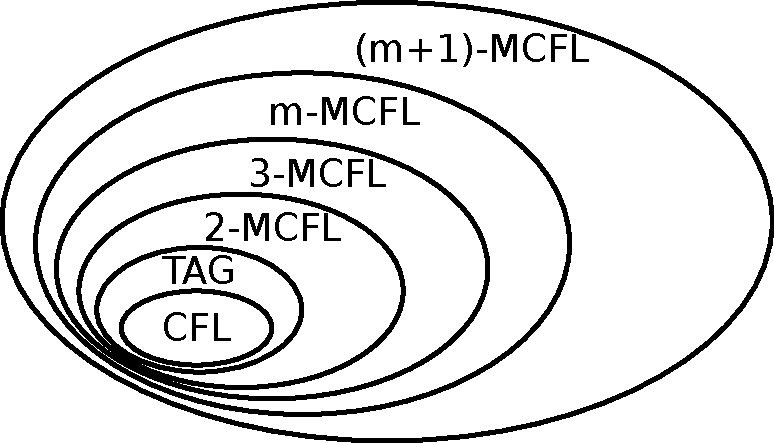
\includegraphics[width=\marginparwidth]{part_02_Foundations/chapter_08_MCFG/figures/mcfg.pdf}
    \caption{Иерархия MCFL по максимальному рангу $m$}
    \label{fig:mcfg_hierarchy_m}
\end{marginfigure}

\begin{theorem}[Иерархия по $r$ для $m=1$]
    \label{thm:hierarchy_r_1}
    \begin{enumerate}
        \item $1$-MCFL = CFL.
        \item $1$-MCFL($1$) $\subsetneq$ $1$-MCFL($2$).
        \item $1$-MCFL($r$) = $1$-MCFL($r+1$) для всех $r \ge 2$.
    \end{enumerate}
\end{theorem}

\begin{theorem}[Иерархия по $r$ для $m=2$~\sidecite{rambow1999independent}]
    \label{thm:hierarchy_r_2}
    $2$-MCFL($2$) = $2$-MCFL($3$).
\end{theorem}

\begin{theorem}[Общий случай~\sidecite{seki1991multiple,rambow1999independent}]
    \label{thm:hierarchy_r_general}
    Если $m > 2$ и $r > 2$, то $m$-MCFL($r$) $\subsetneq$ $m$-MCFL($r+1$).
\end{theorem}

\begin{marginfigure}
    \centering
    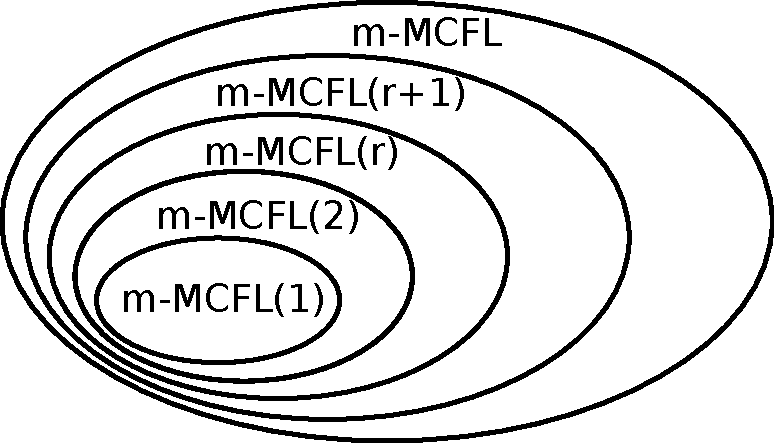
\includegraphics[width=\marginparwidth]{part_02_Foundations/chapter_08_MCFG/figures/mcfg_2.pdf}
    \caption{Иерархия MCFL по максимальной длине правой части $r$}
    \label{fig:mcfg_hierarchy_r}
\end{marginfigure}

Кроме того, известно свойство поглощения ранга: для любых $r \ge 2$ и $k \ge 1$ таких, что $k \le r-2$, имеет место включение
$(m \cdot (k-1))$-MCFL($r-k$) $\subseteq m$-MCFL($r$)~\sidecite{seki1991multiple}.

\section{Свойства замкнутости}
\label{sec:MCFGClosureProperties}
\tikzsetfigurename{MCFG_Closure_}

\mytodo{Замкнутость относительно гомоморфизмов: сверить по Rambow1999, доказывается ли там замкнутость относительно всех трёх операций (гомоморфизм, обратный гомоморфизм, подстановка) или только части.}

\mytodo{Доказательство незамкнутости: конструкция языков $L_1$, $L_2$  нуждается в верификации по Seki1991.}

Свойства замкнутости MCFL во многом аналогичны свойствам контекстно-свободных языков, однако имеются и существенные отличия.

\begin{theorem}[Замкнутость MCFL]
    \label{thm:mcf_closure}
    Класс MCFL замкнут относительно следующих операций:
    \begin{enumerate}
        \item \textbf{Объединение}: если $L_1, L_2 \in MCFL$, то $L_1 \cup L_2 \in MCFL$.
        \item \textbf{Конкатенация}: если $L_1, L_2 \in MCFL$, то $L_1 \cdot L_2 \in MCFL$.
        \item \textbf{Звезда Клини}: если $L_1 \in MCFL$, то $L_1^* \in MCFL$.
        \item \textbf{Пересечение с регулярными языками}: если $L_1 \in MCFL$, а $L_2$~--- регулярный язык, то $L_1 \cap L_2 \in MCFL$.
        \item \textbf{Разность с регулярными языками}: если $L_1 \in MCFL$, а $L_2$~--- регулярный язык, то $L_1 \setminus L_2 \in MCFL$.
        \item \textbf{Гомоморфизм}: если $L_1 \in MCFL$, то $h(L_1) \in MCFL$ для любого гомоморфизма $h$.
        \item \textbf{Обратный гомоморфизм}: если $L_1 \in MCFL$, то $h^{-1}(L_1) \in MCFL$ для любого гомоморфизма $h$.
        \item \textbf{Подстановка}: если $L_1 \in m$-MCFL и для каждого символа $a \in \Sigma$ задан язык $L_a \in m$-MCFL, то результат подстановки также принадлежит $m$-MCFL.
    \end{enumerate}
\end{theorem}

\begin{proof}
    Для каждого пункта приведём конструкцию.

    \begin{enumerate}
        \item Пусть $G_1 = \langle \Sigma_1, N_1, S_1, P_1 \rangle$ и $G_2 = \langle \Sigma_2, N_2, S_2, P_2 \rangle$~--- MCFG для языков $L_1$ и $L_2$ соответственно, с непересекающимися множествами нетерминалов. Грамматика для $L_1 \cup L_2$:
              \[
              G_3 = \langle \Sigma_1 \cup \Sigma_2, N_1 \cup N_2 \cup \{S_3\}, S_3, P_1 \cup P_2 \cup \{ S_3(x_1) \leftarrow S_1(x_1),\ S_3(x_1) \leftarrow S_2(x_1) \} \rangle.
              \]

        \item Конкатенация: $G_3$ получается добавлением правила $S_3(x_1 x_2) \leftarrow S_1(x_1), S_2(x_2)$.

        \item Звезда Клини: $G_2$ получается добавлением правил $S_2(x_1) \leftarrow S_1(x_1)$, $S_2(x_1 x_2) \leftarrow S_2(x_1), S_2(x_2)$.

        \item Пересечение с регулярными языками~--- ключевое свойство для MCFL-достижимости. Построим произведение MCFG $G$ и DFA $A = \langle Q, \Sigma, q_0, \delta, F \rangle$, распознающего регулярный язык. Для каждого нетерминала $N$ ранга $k$ и каждого набора состояний $p_1,\ldots,p_{k+1} \in Q$ введём аннотированный нетерминал $N_{p_1,\ldots,p_{k+1}}$, порождающий кортеж $(w_1,\ldots,w_k)$, если существуют пути $p_1 \xrightarrow{w_1} p_2$, \ldots, $p_k \xrightarrow{w_k} p_{k+1}$ в $A$. Каждое исходное правило преобразуется: все $p_i$ в левой части соединяются с $p_j$ в правой в соответствии с тем, как переменные располагаются в строках $s_1,\ldots,s_k$. Стартовый нетерминал~--- $S_{q_0, q}$ для некоторого $q \in F$.

        \item Разность с регулярным языком: $L_1 \setminus L_2 = L_1 \cap \overline{L_2}$, а регулярные языки замкнуты относительно дополнения.
        \item Гомоморфизм: заменим каждый терминал $a$ в строках $s_i$ правил MCFG на $h(a)$. Полученная грамматика порождает $h(L_1)$.

        \item Обратный гомоморфизм и подстановка: доказательство этих свойств технически более сложно; полное доказательство можно найти в работе~\sidecite{rambow1999independent}\sidenote{В этой работе показано, что $q$-MCFL($r$) для $r \ge 2$ является substitution-closed full AFL.}.
    \end{enumerate}
\end{proof}
\mytodo{Привести доказательство замкнутости относительно обратного гомоморфизма и подстановки, а не только ссылку на Rambow1999.}

\begin{theorem}[Незамкнутость MCFL]
    \label{thm:mcf_nonclosure}
    Класс MCFL \emph{не} замкнут относительно следующих операций:
    \begin{enumerate}
        \item \textbf{Пересечение}: существуют $L_1, L_2 \in MCFL$, такие что $L_1 \cap L_2 \notin MCFL$.
        \item \textbf{Дополнение}: существует $L \in MCFL$, такое что $\overline{L} \notin MCFL$.
        \item \textbf{Разность}: существуют $L_1, L_2 \in MCFL$, такие что $L_1 \setminus L_2 \notin MCFL$.
    \end{enumerate}
\end{theorem}

\begin{proof}
    Для доказательства незамкнутости относительно пересечения рассмотрим языки Секи с соавторами~\sidecite{SEKI1991191}:
    \[
    L_1 = \{\,a_1^n b_1^n a_2^n b_2^n \cdots a_{m+1}^n b_{m+1}^n \mid n \ge 0\,\}, \qquad
    L_2 = \{\,a_1^n a_2^n \cdots a_{m+1}^n b_1^n b_2^n \cdots b_{m+1}^n \mid n \ge 0\,\}.
    \]
    Язык $L_1$ является $(m+1)$-MCFL($1$) (теорема~\ref{thm:hierarchy_m}), язык $L_2$ является $2$-MCFL (строится парой $(a_1^n\cdots a_{m+1}^n,\; b_1^n\cdots b_{m+1}^n)$, каждый компонент которой является КС-языком).
    В работе~\sidecite{SEKI1991191} показано, что $L_1 \cap L_2$ не является MCFL: при надлежащем выборе $m$ ранг, требуемый для порождения пересечения, превосходит $m$, а конструкция допускает масштабирование на произвольно большие значения~--- таким образом, пересечение не принадлежит ни одному из классов $m$-MCFL.

    Незамкнутость относительно дополнения следует из незамкнутости относительно пересечения по законам де Моргана:
    если бы MCFL были замкнуты относительно дополнения, то $L_1 \cap L_2 = \overline{\overline{L_1} \cup \overline{L_2}}$ также был бы MCFL, что неверно.

    Незамкнутость относительно разности следует из незамкнутости относительно пересечения, так как $L_1 \cap L_2 = L_1 \setminus \overline{L_2}$, а $\overline{L_2} \in MCFL$ не гарантировано.
\end{proof}
\mytodo{Привести явное построение 2-MCFG для языка L₂ в доказательстве незамкнутости пересечения.}
\mytodo{Добавить \textbackslash label у конструкций L₁ и L₂.}


\setchapterpreamble[u]{\margintoc}
\chapter{Конъюнктивные и булевы грамматики}
\label{ConjunctiveBoolean}
\tikzsetfigurename{CB_}

Впервые конъюнктивные и булевы грамматики были предложены Александром Охотиным~\cite{DBLP:journals/jalc/Okhotin01,Okhotin:2003:BG:1758089.1758123}. Дадим определение конъюнктивной грамматики.

\section{Конъюнктивные грамматики}
	\tikzsetfigurename{CB_Conjunctive_}

\begin{definition}
    \textit{Конъюнктивной грамматикой} называется $G = (\Sigma,N,P,S)$, где:
    \begin{itemize}
        \item $\Sigma$ и $N$~--- дизъюнктивные конечные непустые множества терминалов и нетерминалов.
        \item $P$~--- конечное множество продукций, каждая вида
        \[
        A\rightarrow \alpha_1\&...\&\alpha_n
        \]
        ,где $A \in N,n \geq 1$ и $\alpha_1,...,\alpha_n \in (\Sigma \cup N)^*$.
        \item $S \in N$ ~--- стартовый нетерминал.
    \end{itemize}
\end{definition}

Конъюнктивная грамматика генерирует строки, выводя их из начального символа, так же, как это происходит в контекстно-свободных грамматиках в параграфе~\ref{chpt:CFG}. Промежуточные строки, используемые в процессе вывода, являются формулами следующего вида:

\begin{definition}\label{def:ConjunctiveFormula}
    Пусть $G = (\Sigma,N,P,S)$~--- конъюнктивная грамматика. Множество конъюнктивных формул $ \mathcal{F}$ определяется индуктивно:
    \begin{itemize}
        \item Пустая строка $\varepsilon$~--- конъюнктивная формула. 
        \item Любой символ из $(\Sigma \cup N)$~--- формула.
        \item Если $\mathcal{A}$ и $\mathcal{B}$ непустые формулы, тогда $\mathcal{AB}$~--- формула.
        \item Если $\mathcal{A}_1,\ldots,\mathcal{A}_n$ $(n \geqslant 1)$~--- формула, тогда $(\mathcal{A}_1\&\ldots\&\mathcal{A}_n)$~--- формула.
    \end{itemize}
\end{definition}

\begin{definition}
    Пусть $G = (\Sigma,N,P,S)$~--- конъюнктивная грамматика. Аналогично определению отношения непосредственной выводимости в контекстно-свободной грамматике~\ref{def:CFGDerivability} определим $\xRightarrow[G]{}$ как отношение непосредственной выводимости на множестве конъюнктивных формул.
    \begin{itemize}
        \item Любой нетерминал в любой формуле может быть перезаписан телом любого правила для этого терминала заключенным в скобки. То есть для любых $s^{'},s^{''} \in (\Sigma \cup N \cup \{(, \&, )\})^*$ и $A\in N$, таких что $s^{'}As^{''}$~--- формула, и для всех правил вида $A \rightarrow \alpha_1\&\ldots\&\alpha_n \in P$, имеем $s^{'}As^{''}\xRightarrow[G]{}s^{'}(\alpha_1\&\ldots\&\alpha_n)s^{''}$. 
        \item Если формула содержит подформулу в виде конъюнкции одной или нескольких одинаковых терминальных строк, заключенных в скобки, тогда подформула может быть перезаписана терминальной строкой без скобок. То есть для любых $s^{'},s^{''} \in (\Sigma \cup N \cup \{(, \&, )\})^*$, $(n \geqslant 1)$ и $w \in \Sigma^*$, таких что $s^{'}(w\&\ldots\&w)s^{''}$~--- формула, имеем $s^{'}(w\&\ldots\&w)s^{''}\xRightarrow[G]{}s^{'}ws^{''}$.
    \end{itemize}
    Как и в случае контекстно-свободной грамматики обозначим $\xRightarrow[G]{}^*$ рефлексивное транзитивное замыкание отношения $\xRightarrow[G]{}$.
\end{definition}

\begin{definition}
    Пусть $G = (\Sigma,N,P,S)$~--- конъюнктивная грамматика. Язык, порождаемый формулой, это множество всех терминальных строк выводимых из этой формулы: $L_{G}(\mathcal{A}) = \{w\in\Sigma^* \mid \mathcal{A} \xRightarrow[G]{}^*w\}$. Очевидно, что язык порождаемый грамматикой, это язык порождаемый стартовым нетерминалом $S$ : $L(G) = L_{G}(S) = L(S)$.
\end{definition}

\begin{theorem}\label{thm:ConjunctiveFormulaLanguage}
    Пусть $G = (\Sigma,N,P,S)$~--- конъюнктивная грамматика. Пусть $\mathcal{A}_1,\ldots,\mathcal{A}_n,\mathcal{B}$~--- формулы, $A \in N$, $a \in \Sigma$. Тогда,
    \begin{enumerate}
        \item $L(\varepsilon) = \{\varepsilon\}$.
        \item $L(a) = \{a\}$.
        \item $L(A) = \bigcup_{A \rightarrow \alpha_1\&\ldots\&\alpha_n \in P} L((\alpha_1\&\ldots\&\alpha_m))$.
        \item $L(\mathcal{AB}) = L(\mathcal{A})*L(\mathcal{B})$
        \item $L((\mathcal{A}_1\&\ldots\&\mathcal{A}_n)) = \bigcap_{i = 1}^{n}L(\mathcal{A}_i)$.
    \end{enumerate}
\end{theorem}

Теорема~\ref{thm:ConjunctiveFormulaLanguage} уже подразумевает интерпретацию грамматики как системы уравнений. Используем математический подход, чтобы лучше охарактеризовать конъюнктивные языки с помощью систем уравнений.

\begin{definition}[Выражение]
    Пусть $\Sigma$ конечный непустой алфавит. Пусть $X = \{X_1,\ldots,X_N\}$ вектор переменных. Выражение над алфавитом $\Sigma$, зависящее от переменных $X$, определяется индуктивно:
    \begin{itemize}
       \item $\varepsilon$~--- выражение.
       \item Любой символ $a\in\Sigma$~--- выражение.
       \item Любая переменная $X_i\in X$~--- выражение.
       \item Если $\phi_1$ и $\phi_2$ выражения, то $\phi_1\phi_2, (\phi_1\mid\phi_2), (\phi_1\&\phi_2)$ также выражения.
    \end{itemize}
    Заметим, что любая формула, в терминах определения~\ref{def:ConjunctiveFormula}, является выражением, где нетерминалы формулы это переменные выражения. С другой стороны, любое выражение, не содержащее дизъюнкции, формула.
\end{definition}

Предположим, что переменные $X_i$ приняли в качестве значений слова из языка над алфавитом $\Sigma$. Определим значение всего выражения.

\begin{definition}[Значение выражения]\label{def:ConjunctiveExpressionValue}
    Пусть $L = (L_1,\ldots,L_n) (L_i \subseteq \Sigma^*)$ вектор из $n$ языков над $\Sigma$, где $n \geqslant 1$. Пусть $\phi$ выражение над $\Sigma$, зависящее от переменных $X_1,\ldots,X_n$. Значение выражения $\phi$ на векторе $L$~--- это язык над тем же алфавитом $\Sigma$. Обозначим его $\phi(L)$ и определим индуктивно на структуре выражения:
    \begin{itemize}
       \item $\varepsilon(L) = \{\varepsilon\}$.
       \item $a(L) = \{a\}$ для любого $a\in\Sigma$.
       \item $X_i(L) = L_i$ для любого $X_i \in X$.
       \item $\phi_1\phi_2 = \phi_1(L) * \phi_2(L), (\phi_1\mid\phi_2)(L) = \phi_1(L) \cup \phi_2(L), (\phi_1\&\phi_2)(L) = \phi_1(L) \cap \phi_2(L)$ для любых выражений $\phi_1$ и $\phi_2$.
    \end{itemize}
\end{definition}

Обобщим определение~\ref{def:ConjunctiveExpressionValue} на случай вектора выражений.

\begin{definition}[Значение вектора выражений]
    Пусть $L = (L_1,\ldots,L_n) (L_i \subseteq \Sigma^*)$ вектор из $n$ языков над $\Sigma$, где $n \geqslant 1$. Пусть $\phi_1,\ldots,\phi_m$ выражения над $\Sigma$, зависящее от переменных $X_1,\ldots,X_n$. Значение вектора выражений $P = (\phi_1,\ldots,\phi_m)$ на векторе $L$~--- это вектор языков $P(L) = (\phi_1(L),\ldots,\phi_m(L))$ над тем же алфавитом $\Sigma$. 
\end{definition}

Зададим частичный порядок относительно включения $``\preccurlyeq''$ на множестве языков и расширим его на векторы языков длины $n$: $(L_1^{'},\ldots,L_n^{'})\preccurlyeq(L_1^{''},\ldots,L_n^{''})$ тогда и только тогда, когда $L_i^{'} \subseteq L_i^{''}$ для любого $1\leqslant i \leqslant n$

\begin{definition}\label{def:ConjunctiveEquationSystem}
   $X = P(X)$ система уравнений над алфавитом $\Sigma$ и $X = \{X_1,\ldots,X_n\}$, где $P = (\phi_1,\ldots,\phi_n)$ вектор выражений над алфавитом $\Sigma$, зависящий от $X$.
   
   Вектор языков $L = (L_1,\ldots,L_n)$ является решением системы уравнений если $L = P(L)$.
   
   Наименьшее решение $L$ это вектор языков, такой что для любого другого сравнимого вектора языков $L^{'}$ выполняется $L \preccurlyeq L^{'}$.
\end{definition}

Заметим, что оператор $P$ на множестве $2^{\Sigma}\times\ldots\times2^{\Sigma}$, что решение системы~\ref{def:ConjunctiveEquationSystem} это неподвижная точка $P$ и что наименьшее решение системы это наименьшая неподвижная точка оператора $P$.

\begin{theorem}\label{thm:LeastFixedPoint}
    Для любой системы из определения~\ref{def:ConjunctiveEquationSystem} с переменными $X_1,\ldots,X_n$, оператор $P = (\phi_1,\ldots,\phi_n)$ имеет наименьшую неподвижную точку $L = (L_1,\ldots,L_n) = \lim_{i\to\infty}P^{i}\underbrace{(\varnothing,\ldots,\varnothing)}_n$.
\end{theorem}

Приведем пример конъюнктивной грамматики.

\begin{example}[Пример конъюнктивной грамматики]
    Следующая конъюнктивная грамматика $G$ порождает язык $\{a^nb^nc^n\mid n \geq 0\}$:
    
    \begin{align*}
    1.\ S   &\to A B \& D C \\
    2.\ A  &\to a A \mid \varepsilon \\ 
    3.\ B &\to b B c \mid \varepsilon \\
    4.\ C   &\to c C \mid \varepsilon \\ 
    5.\ D   &\to aDb \mid \varepsilon
    \end{align*}
    
    Легко видеть, что $L(AB) = \{a^ib^jc^k\mid j = k\}$ и $L(DC) = \{a^ib^jc^k\mid i = j\}$. Тогда $L(S) = L(AB) \cap L(DC) = \{a^nb^nc^n\mid n \geq 0\}$. 
    
    В этой грамматике строка $abc$ может быть получена следующим образом. Для начала представим грамматику в виде системы уравнений:
    \begin{align*}
    S &= A B \cap D C \\ 
    A &= \{a\}A \cup \varepsilon \\ 
    B &= \{b\}B\{c\} \cup \varepsilon \\
    C &= \{c\}C \cup \varepsilon \\ 
    D &= \{a\}D\{b\} \cup \varepsilon
    \end{align*}
    Используя теорему~\ref{thm:LeastFixedPoint}, будем итеративно вычислять $P^{i}\underbrace{(\varnothing,\ldots,\varnothing)}_5$. На каждом шаге будем подставлять все терминальные строки из языков, порожденных нетерминалами на предыдущем шаге, в соответствующие нетерминалы правой части каждого уравнения и записывать получившиеся терминальные строки в языки нетерминалов текущего шага. Продолжаем до тех пор пока язык, порождаемый нетерминалом $S$, не будет содержать терминальную строку $``abc''$.
    \begin{enumerate}
        \item На начальном этапе имеем $P^{0}(\varnothing,\ldots,\varnothing) = (S: \varnothing, A: \varnothing, B: \varnothing, C: \varnothing, D: \varnothing)$ 
        \item Подставляем в первое уравнение терминальные строки из шага 1 в соответствующие нетерминалы, т.е. 
        \begin{align*}
            S:  \varnothing &= \varnothing\varnothing \cap \varnothing\varnothing \\ 
            A: \{\varepsilon\} &= \{a\}\varnothing \cup \{\varepsilon\} \\ 
            B: \{\varepsilon\} &= \{b\}\varnothing\{c\} \cup \{\varepsilon\} \\
            C: \{\varepsilon\} &= \{c\}\varnothing \cup \{\varepsilon\} \\ 
            D: \{\varepsilon\} &= \{a\}\varnothing\{b\} \cup \{\varepsilon\}
        \end{align*}
        В конце итерации получаем $P^{1}(\varnothing,\ldots,\varnothing) = (S: \varnothing, A: \{\varepsilon\}, B: \{\varepsilon\}, C: \{\varepsilon\}, D: \{\varepsilon\})$
        \item Делаем еще одну итерацию,
        \begin{align*}
            S:  \{\varepsilon\} &= \{\varepsilon\}\{\varepsilon\} \cap \{\varepsilon\}\{\varepsilon\} \\ 
            A: \{a, \varepsilon\} &= \{a\}\{\varepsilon\} \cup \{\varepsilon\} \\ 
            B: \{bc, \varepsilon\} &= \{b\}\{\varepsilon\}\{c\} \cup \{\varepsilon\} \\
            C: \{c, \varepsilon\} &= \{c\}\{\varepsilon\} \cup \{\varepsilon\} \\ 
            D: \{ab, \varepsilon\} &= \{a\}\{\varepsilon\}\{b\} \cup \{\varepsilon\}
        \end{align*}
        В конце итерации получаем $P^{2}(\varnothing,\ldots,\varnothing) = (S: \{\varepsilon\}, A: \{a, \varepsilon\}, B: \{bc, \varepsilon\}, C: \{c, \varepsilon\}, D: \{ab, \varepsilon\})$
        \item Еще одна итерация,
        \begin{align*}
            S:  \{\fbox{abc}, \varepsilon\} &= \{a, \varepsilon\}\{bc, \varepsilon\} \cap \{ab, \varepsilon\}\{c, \varepsilon\} \\ 
            A: \{a, aa, \varepsilon\} &= \{a\}\{a, \varepsilon\} \cup \{\varepsilon\} \\ 
            B: \{bc, bbcc, \varepsilon\} &= \{b\}\{bc, \varepsilon\}\{c\} \cup \{\varepsilon\} \\
            C: \{c, cc, \varepsilon\} &= \{c\}\{c, \varepsilon\} \cup \{\varepsilon\} \\ 
            D: \{ab, aabb, \varepsilon\} &= \{a\}\{ab, \varepsilon\}\{b\} \cup \{\varepsilon\}
        \end{align*}
        В конце итерации получили $P^{3}(\varnothing,\ldots,\varnothing) = (S: \{\fbox{abc}, \varepsilon\}, A: \{a, aa, \varepsilon\}, B: \{bc, bbcc, \varepsilon\}, C: \{c, cc, \varepsilon\}, D: \{ab, aabb, \varepsilon\})$. Заметим, что терминальная строка $``abc"$ появилась в языке, который порождает стартовый нетерминал $S$. Т.е. терминальная строка $``abc"$ выводима в грамматике $G$, что и требовалось показать.
    \end{enumerate}
    
    Заметим, что строку $``abc"$ также можно получить применением правил вывода. здесь цифра над стрелкой соответствует номеру примененного правила. 
    \begin{align*}
        S &\xRightarrow{1}(AB\&DC) \\
        &\xRightarrow{2}(aAB\&DC) \xRightarrow{2} (a\varepsilon B\&DC) \\
        &\xRightarrow{3}(abBc\&DC) \xRightarrow{3}(ab\varepsilon c\&DC) \\
        &\xRightarrow{5}(abc\&aDbC) \xRightarrow{5}(abc\&a\varepsilon bC) \\
        &\xRightarrow{4}(abc\&abcC) \xRightarrow{4}(abc\&abc\varepsilon) \\
        &\Rightarrow(abc\&abc) \Rightarrow abc
    \end{align*}
\end{example}

\begin{example}
    Конъюнктивная грамматика $G$ для языка $L = \{wcw \mid w \in \{a, b\}^*\}$:
    \begin{align*}
    S &\to C \& D \\ 
    C &\to aCa \mid aCb \mid bCa \mid bCb \mid c \\ 
    D &\to aA\&aD \mid bB\&bD \mid cE \\
    A &\to aAa \mid aAb \mid bAa \mid bAb \mid cEa \\
    B &\to aBa \mid aBb \mid bBa \mid bBb \mid cEb \\
    E &\to aE \mid bE \mid \varepsilon
    \end{align*}
\end{example}

Подробнее о конъюнктивных грамматиках можно прочитать в статьях~\cite{DBLP:journals/jalc/Okhotin01, Okhotin2002, DBLP:journals/tcs/Okhotin03a, f60a33d409364914be560cac0e54b12c}.

Определим бинарную нормальную форму конъюнктивной грамматики.

\begin{definition}[Бинарная нормальная форма]
    Конъюнктивная грамматика $G = (\Sigma, N, P, S)$ находится в бинарной нормальной форме, если каждое правило из $P$ имеет один из следующих видов:
    \begin{itemize}
        \item $A \rightarrow B_1 C_1 \& \ldots \& B_m C_m$, где $m \geqslant 1$ и $A,B_i,C_i \in N$;
        \item $A \rightarrow a$, где $A \in N$ и $a \in \Sigma$;
        \item $S \rightarrow \varepsilon$, если только $S$ не содержится в правой части ни одного правила.
    \end{itemize}
\end{definition}

\begin{theorem}\label{thm:BinaryNormalForm}
    Для каждой конъюнктивной грамматики $G$ можно построить конъюнктивную грамматику в бинарной нормальной форме $G^{'}$, такую что $L(G) = L(G^{'})$.
\end{theorem}

Доказательство теоремы~\ref{thm:BinaryNormalForm} описано в статье~\sidecite{DBLP:journals/jalc/Okhotin01}.

\section{Булевы грамматики}

Дадим определение булевой грамматики.

\begin{definition}
    \textit{Булевой грамматикой} называется $G = (\Sigma,N,P,S)$, где:
    \begin{itemize}
        \item $\Sigma$ и $N$ --- дизъюнктивные конечные непустые множества терминалов и нетерминалов.
        \item $P$ --- конечное множество продукций, каждая вида
        \[
        A\rightarrow \alpha_1\&...\&\alpha_m\&\neg\beta_1\&...\&\neg\beta_n
        \]
        ,где $A \in N, m, n >=0, m+n \geq 1$ и $\alpha_i,\beta_j \in (\Sigma \cup N)^*$.
        \item $S \in N$  --- стартовый нетерминал.
    \end{itemize}
\end{definition}

Приведем пример булевой грамматики.

\begin{example}
    Следующая булева грамматика порождает язык  $\{a^mb^nc^n\mid m,n \geq 0, m \neq n \}$:
    
    \begin{align*}
    S   &\to A B \& \neg D C \\ 
    A  &\to a A \mid \varepsilon \\ 
    B &\to b B c \mid \varepsilon \\
    C   &\to c C \mid \varepsilon \\ 
    D   &\to aDb \mid \varepsilon
    \end{align*}
    
    Очевидно, что $L(AB) = \{a^mb^nc^n\mid m,n \in \mathbb{N}\}$ и $L(DC) = \{a^nb^nc^m\mid m,n \in \mathbb{N}\}$. Тогда $L(AB)\cap\overline{L(DC)} = \{a^mb^nc^n\mid m,n \geq 0, m \neq n \}$.
\end{example}

Подробнее о булевых грамматиках можно прочитать в статьях~\cite{Okhotin:2003:BG:1758089.1758123,Okhotin:2014:PMM:2565359.2565379}.

Определим бинарную нормальную форму конъюнктивной грамматики.
\begin{definition}[Бинарная нормальная форма]
    Конъюнктивная грамматика $G = (\Sigma, N, P, S)$ находится в бинарной нормальной форме, если каждое правило из P имеет вид,
    \begin{itemize}
        \item $A \rightarrow B_1 C_1 \& \ldots\& B_m C_m$, где $m \geqslant 1; A,B_i,C_i \in N$.
        \item $A \rightarrow a$, где $A \in N, a \in \Sigma$.
        \item $S \rightarrow \varepsilon$, если только $S$ не содержится в правой части всех правил.
    \end{itemize}
\end{definition}

\begin{theorem}\label{Binary normal form conjunctive grammar theorem}
    Для каждой конъюнктивной грамматики $G$ можно построить конъюнктивную грамматику в бинарной нормальной форме $G^{'}$, такую что $L(G) = L(G^{'})$.
\end{theorem}
Доказательство теоремы~\ref{Binary normal form conjunctive grammar theorem} описано в статье~\cite{DBLP:journals/jalc/Okhotin01}.



\addpart{Анализ графов с использованием формальных языков в качестве ограничений на пути}
    \tikzsetfigurename{Part03_GraphAnalysis_}
    \label{part:GraphAnalysis}

\setchapterpreamble[u]{\margintoc}
\chapter[Пути с ограничениями в терминах формальных языков]{Задача анализа графов с использованием формальных языков в качестве ограничений на пути}
\label{chpt:FLPQ}
\tikzsetfigurename{FLPQ_}

\mytodo{Переработать всю главу.}

В данной главе сформулируем постановку задачи о поиске путей в графе с ограничениями.
Также мы приведём несколько примеров областей, в которых применяются алгоритмы решения этой задачи.

\section{Постановка задачи}

Пусть нам дан конечный ориентированный помеченный граф $\mscrG = \langle V, E, L \rangle$.
Функция $\omega(\pi) = \omega((v_0, l_0, v_1), (v_1, l_1, v_2), \dots, (v_{n-1}, l_{n-1}, v_n)) = l_0 \cdot l_1 \cdot \dots \cdot l_{n-1}$ строит слово по пути посредством конкатенации меток рёбер вдоль этого пути.
Очевидно, для пустого пути данная функция будет возвращать пустое слово, а для пути длины $n  > 0$~--- непустое слово длины $n$.

Если теперь рассматривать задачу поиска путей, то окажется, что то множество путей, которое мы хотим найти, задаёт множество слов, то есть язык.
А значит, критерий поиска мы можем сформулировать следующим образом: нас интересуют такие пути, что слова, составленные из меток вдоль них, принадлежат заданному языку.

\begin{definition}[Задача поиска путей с ограничениями в терминах формальных языков]
    \label{def1}
    \emph{Задача поиска путей с ограничениями в терминах формальных языков} заключается в поиске множества путей $\Pi = \{\pi \mid \omega(\pi) \in \mscrL\}$.
\end{definition}

В задаче поиска путей мы можем накладывать дополнительные ограничения на путь (например, чтобы он был простым, кратчайшим или Эйлеровым~\sidecite{kupferman2016eulerian}), но это уже другая история.

Другим вариантом постановки задачи является задача достижимости.

\begin{definition}[Задача достижимости]
    \label{def2}
    \emph{Задача достижимости} заключается в поиске множества пар вершин, для которых найдется путь с началом и концом в этих вершинах, что слово, составленное из меток рёбер пути, будет принадлежать заданному языку
    \[\Pi' = \{(v_{i}, v_{j}) \mid \exists v_{i} \pi v_{j}, \omega(\pi) \in \mscrL\}.\]
\end{definition}

При этом, множество $\Pi$ может являться бесконечным, тогда как $\Pi'$ конечно, по причине конечности графа $\mscrG$.

Язык $\mscrL$ может принадлежать разным классам и быть задан разными способами.
Например, он может быть регулярным, контекстно-свободным, или многокомпонентным контекстно-свободным.

Если $\mscrL$~--- регулярный, $\mscrG$ можно рассматривать как недетерминированный конечный автомат (НКА), в котором все вершины являются одновременно и стартовыми, и конечными.
Тогда задача поиска путей, в которой $\mscrL$~--- регулярный, сводится к пересечению двух регулярных языков.

Более подробно мы рассмотрим случай, когда $\mscrL$~--- контекстно-свободный язык.

Путь $G = \langle \Sigma, N, P \rangle$~--- контекстно-свободная грамматика.
Будем считать, что $L \subseteq \Sigma$.
Мы не фиксируем стартовый нетерминал в определении грамматики, поэтому, чтобы описать язык, задаваемый ей, нам необходимо отдельно зафиксировать стартовый нетерминал.
Таким образом, будем говорить, что $L(G,N_i) = \{ w \mid N_i \xRightarrow[G]{*} w  \}$~--- это язык задаваемый грамматикой $G$ со стартовым нетерминалом $N_i$.

\begin{example}
    Пример задачи поиска путей.

    Дана грамматика $G$, задающая язык $\mscrL = a^n b^n$:
    \begin{align*}
        S & \to a b   \\
        S & \to a S b
    \end{align*}
    И дан граф $\mscrG$, представленный на рисунке~\ref{fig:all_paths_example}.
\begin{marginfigure}
    \begin{center}
        \input{figures/edge_labelled_graph_a_3_loop_b_2_loop}
    \end{center}
    \caption{Входной граф}
    \label{fig:all_paths_example}
\end{marginfigure}

    Кратчайшими путями, принадлежащими множеству $\Pi = \{\pi \mid \omega(\pi) \in \mscrL\}$, являются, например, пути, представленные на изображении~\ref{fig:paths}.

\begin{marginfigure}
    \begin{center}
        \input{part_03_GraphAnalysis/chapter_10_FLPQ/figures/path1}
        \input{part_03_GraphAnalysis/chapter_10_FLPQ/figures/path2}
    \end{center}
    \caption{Примеры путей}
    \label{fig:paths}
\end{marginfigure}

\end{example}

\section{О разрешимости задачи}
	\label{sec:FLPQ_Decidability}
	\tikzsetfigurename{FLPQ_Decidability_}

Задачи из определения~\ref{def:FLPQ} и~\ref{def:Reachability} сводятся к построению пересечения языка $\mscrL$ и языка, задаваемого путями графа, $R$.
А мы для обсуждения разрешимости задачи рассмотрим более слабую постановку задачи:

\mytodo{Придумать осмысленное название определения}
\begin{definition}[TODO: Что ты?]
    Необходимо проверить, что существует хотя бы один такой путь $\pi$ для данного графа, для данного языка $\mscrL$, что $\omega(\pi) \in \mscrL$.
\end{definition}

Эта задача сводится к проверке пустоты пересечения языка $\mscrL$ c $R$~--- регулярным языком, задаваемым графом.
От класса языка $\mscrL$ зависит её разрешимость:
\begin{itemize}
    \item Если $\mscrL$ регулярный, то получаем задачу пересечения двух регулярных языков: $\mscrL \cap R = R'$.
          $R'$~--- также регулярный язык.
          Проверка регулярного языка на пустоту~--- разрешимая проблема.
    \item Если $\mscrL$ контекстно-свободный, то получаем задачу: $\mscrL \cap R = CF$~--- контекстно-свободный.
          Проверка контекстно-свободного языка на пустоту~--- разрешимая проблема.
    \item Помимо иерархии Хомского существуют и другие классификации языков.
          Так например, класс конъюнктивных (Conj) языков~\sidecite{DBLP:journals/jalc/Okhotin01}является строгим расширением контекстно-свободных языков и все так же позволяет полиномиальный синтаксический анализ.

          Пусть $\mscrL$~--- конъюнктивный.
          При пересечении конъюнктивного и регулярного языков получается конъюнктивный ($\mscrL \cap R = Conj$), а проблема проверки Conj на пустоту не разрешима~\sidecite{DBLP:journals/tcs/Okhotin03a}.
    \item Ещё один класс языков из альтернативной иерархии, не сравнимой с Иерархией Хомского,~--- MCFG (multiple context-free grammars)~\sidecite{SEKI1991191}.
          Как его частный случай~--- TAG (tree adjoining grammar)~\sidecite{Joshi1997}.

          Если $\mscrL$ принадлежит классу MCFG, то $\mscrL \cap R$ также принадлежит MCFG.
          Проблема проверки пустоты MCFG разрешима~\sidecite{SEKI1991191}.
\end{itemize}

Существует ещё много других классификаций языков, но поиск универсальной иерархии до сих пор продолжается.

Далее, для изучения алгоритмов решения, нас будет интересовать задача $R \cap CF$.

\section{О представимости решения}
	\label{sec:FLPQ_SolutionRepresentation}
	\tikzsetfigurename{FLPQ_SolutionRepr_}

\section{Регулярные языки в качестве ограничений на пути}

Через тензорное произведение.

Классическое построение пересечения автоматов строит их тензорное произведение.

Так как мы хотим отвечать ещё и на вопрос о достижимости, что нам надо ещё и транзитивное замыкание посчитать.

\section{Контекстно-свободные языки в качестве ограничений на пути}
	\label{sec:FLPQ_CFConstraints}
	\tikzsetfigurename{FLPQ_CFConstr_}

\mytodo{Сократить секцию: вынести детали построения грамматики по SPPF в главу 12}

В данной главе мы дадим обзор задачи достижимости с ограничениями в виде контекстно-свободных языков.
Будут рассмотрены история вопроса, области применения, уточнена формальная постановка для КС-случая и описана общая идея адаптации классических алгоритмов синтаксического анализа к графам.



Задача достижимости с ограничениями в виде контекстно-свободных языков была впервые сформулирована Михалисом Яннакакисом в 1990~году в контексте теории баз данных~\sidecite{Yannakakis}.
Немногим позже Репс с соавторами~\sidecite{10.1145/199448.199462} показал, что широкий класс задач межпроцедурного анализа потока данных может быть точно решён в полиномиальное время путём сведения к достижимости на графах с КС-ограничениями.
Этот подход получил название <<достижимость с ограничениями в виде контекстно-свободных языков>> (\emph{Context-Free Language reachability}, CFL-r) и стал одним из основных инструментов статического анализа программ.
Репс~\sidecite{Reps} предложил общую формулировку межпроцедурного анализа в терминах достижимости на графах.
С тех пор CFL-r активно развивается; современный обзор алгоритической перспективы области представлен Павлогяннисом~\sidecite{10.1145/3583660.3583664}.
Систематическое экспериментальное исследование различных алгоритмов поиска путей с КС-ограничениями (CFPQ) проведено Кёйперсом и~др.~\sidecite{Kuijpers:2019:ESC:3335783.3335791}.

Ключевой прикладной областью CFL-r является межпроцедурный статический анализ кода: задачи анализа формулируются как вопросы достижимости в графе зависимостей программы.
Среди конкретных задач~--- анализ алиасов и указателей~\sidecite{Zheng,10.1145/2001420.2001440,DBLP:conf/asplos/WangHZXS17}, анализ загрязнения~\sidecite{huang2015scalable}, анализ потока меток~\sidecite{LabelFlowCFLReachability}, определение мест исправления ошибок по результатам анализа~\sidecite{CFLfinding} и вывод спецификаций~\sidecite{specificationCFLReachability}.
В биоинформатике КС-достижимость применяется для запросов подграфов в биологических графах~\sidecite{cfpqBio}.
В области семантических веб-технологий и RDF-хранилищ КС-ограничения используются для расширения выразительной силы языков запросов; одним из первых таких расширений является cfSPARQL~\sidecite{10.1007/978-3-319-46523-4_38}.
Нисходящие и матричные методы для КС-запросов к RDF-графам развиваются Медейросом и~др.~\sidecite{MEDEIROS201975,MEDEIROS2022101089}.
Анализ происхождения данных в контексте КС-достижимости рассматривается Миао и Деспанде~\sidecite{MiaoProvenance}.
В системах графовых баз данных, таких как Neo4j~\sidecite{Kuijpers:2019:ESC:3335783.3335791} и RedisGraph~\sidecite{10.1145/3398682.3399163}, ведутся работы по интеграции алгоритмов КС-достижимости в промышленные СУБД.


\mytodo{Уточнение формальной постановки для КС-случая}
Пусть дан граф $\mscrG = \langle V, E, L \rangle$ и КС-грамматика $G = \langle \Sigma, N, P, S \rangle$, где $L \subseteq \Sigma$.
Задача достижимости: найти множество пар вершин $(v_i, v_j)$, для которых существует путь $\pi$, такой что $\omega(\pi) \in L(G)$.
Альтернативно: для заданных множеств стартовых и финальных вершин.

\subsection{Общая идея адаптации алгоритмов синтаксического анализа к графам}

\mytodo{Ключевая идея~--- замена позиций в строке на вершины графа}
При обработке терминала в строке есть ровно один следующий символ; в графе~--- несколько исходящих рёбер (конфликт типа shift-shift).
Алгоритмы должны обрабатывать все возможные продолжения.
\mytodo{Исправить ссылки: chpt:CFPQ\_CYK $\to$ chpt:CFPQ, chpt:MatrixBasedAlgos и chpt:MCFLPQ не существуют}
Различные стратегии обработки этого конфликта приводят к различным алгоритмам КС-достижимости (гл.~\ref{chpt:CFPQ_CYK}, раздел~\ref{sec:CFPQ_GLR}, а также гл.~\ref{chpt:MatrixBasedAlgos}--\ref{chpt:MCFLPQ}).

\mytodo{Переиспользовать сквозной граф из секции~\ref{sec:FLPQ_ProblemStatement} вместо fig\_input-graph}
Проиллюстрируем идею на примере поиска путей в графе с использованием рекурсивного автомата и наивной стратегии вычислений.
\begin{marginfigure}
    \begin{center}
        \resizebox{\marginparwidth}{!}{
            \input{part_03_GraphAnalysis/chapter_10_FLPQ/figures/05_CFConstraints/fig_example-rsm.tex}
        }
    \end{center}
    \caption{Расширенный рекурсивный автомат для грамматики $S \to a \ b \mid a \ S \ b$}
    \label{fig:cfpq-rsm-example}
\end{marginfigure}

\begin{marginfigure}
    \begin{center}
        \input{part_03_GraphAnalysis/chapter_10_FLPQ/figures/05_CFConstraints/fig_input-graph.tex}
    \end{center}
    \caption{Пример входного графа}
    \label{fig:cfpq-input-graph}
\end{marginfigure}

Пусть на вход подан граф $D$, представленный на рисунке~\ref{fig:cfpq-input-graph}, а грамматика $G$ содержит два правила $S \to a \ b \mid a \ S \ b$.
Расширенный рекурсивный автомат для данной грамматики показан на рисунке~\ref{fig:cfpq-rsm-example}.
Стартовая вершина~--- $v_0$, наша цель~--- найти хотя бы один путь в каждую достижимую (относительно $G$) вершину.

Начальная конфигурация~--- $(q_4,v_0,[])$: мы начинаем из начального состояния блока для $S'$, начальная позиция в графе~--- стартовая вершина $v_0$, стек пуст. На каждом шаге мы применяем правила из определения~\ref{def:rsm_transition} для вычисления новых конфигураций. Последовательность переходов, представленная ниже, позволяет найти путь \[ v_0 \xrightarrow{a} v_0 \xrightarrow{b} v_1 \]
из $v_0$ в $v_1$ (шаг~\ref{eq:cfpq-rsm-step-res-1}) и путь
\[ v_0 \xrightarrow{a} v_0 \xrightarrow{a} v_0 \xrightarrow{b} v_1 \xrightarrow{b} v_0 \]
из $v_0$ в себя (шаг~\ref{eq:cfpq-rsm-step-res-2}).

\begin{align}
    \setcounter{equation}{0}
    (q_4,v_0,[])     \vdash           & \{(q_0,v_0,[q_5])\}                                                   \\
    (q_0,v_0,[q_5])  \vdash           & \{(q_1,v_0,[a,q_5])\}                                                 \\
    (q_1,v_0,[a,q_5])\vdash           & \{(q_0,v_0,[q_2,a,q_5]) \nonumber                                     \\
                                      & , (q_3,v_1,[b,a,q_5])\}                                               \\
    (q_0,v_0,[q_2,a,q_5]) \vdash      & \{(q_1,v_0,[a,q_2,a,q_5])\}                                           \\
    (q_3,v_1,[b,a,q_5])   \vdash      & \boxed{\{(q_5,v_1,[S(a,b)])\}} \label{eq:cfpq-rsm-step-res-1}        \\
    (q_1,v_0,[a,q_2,a,q_5]) \vdash    & \{(q_3,v_1,[b,a,q_2,a,q_5]) \nonumber                                 \\
                                      & , (q_0,v_0,[q_2,a,q_2,a,q_5])\} \label{eq:cfpq-rsm-step-6}           \\
    (q_3,v_1,[b,a,q_2,a,q_5]) \vdash  & \{(q_2,v_1,[S(a,b),a,q_5])\}                                          \\
    (q_2,v_1,[S(a,b),a,q_5]) \vdash   & \{(q_3,v_0,[b,S(a,b),a,q_5])\}                                        \\
    (q_3,v_0,[b,S(a,b),a,q_5]) \vdash & \boxed{\{(q_5,v_0,[S(a,S(a,b),b)])\}} \label{eq:cfpq-rsm-step-res-2}
\end{align}

Заметим, что у нас нет условий для остановки вычислений, из-за чего в нашем примере можно продолжить вычисления и получить новые пути между $v_0$ и $v_1$.
Более того, можно заметить, что таких путей бесконечное количество, а выбор следующего шага не является детерминированным.
Например, можно выбрать конфигурацию $(q_0,v_0,[q_2,a,q_2,a,q_5])$ для продолжения вычислений после шага~\ref{eq:cfpq-rsm-step-6} с риском попасть в бесконечный цикл, но выбрав $(q_3,v_1,[b,a,q_2,a,q_5])$, мы получим новый путь.


\subsection{Представление всех путей: SPPF для графов}

Теоретические основы SPPF изложены в разделе~\ref{sec:SPPF} главы~\ref{chpt:CFG}.
Здесь мы рассмотрим применение SPPF для представления результатов КС-запросов к графам.

Мы, кроме традиционного использования, будем применять SPPF для представления результатов КС запросов к графам.

В графе может существовать множество способов получить путь из одной вершины в другую. И точно так же при построении деревьев вывода путей может появиться несколько одинаковых нетерминалов, получаемых в разных деревьях по-разному. При объединении в SPPF может оказаться, что какой-то путь из вершины $a$ в вершину $b$ является подпутем другого пути из вершины $a$ в вершину $b$, просто более длинного. То есть появятся циклические зависимости.

\begin{example}
    Рассмотрим пример SPPF для задачи поиска путей с КС ограничениями.
    Пусть дан граф $\mathcal{G}:$

    \begin{center}
       \input{figures/edge_labelled_graph_a_3_loop_b_2_loop}
    \end{center}

    Дана грамматика

    \begin{align*}
        G = \langle \{a,b\}, \{S\},  S, \ & \{ \\
            & \ \ (0)\ S  \to a \ S \ b, \\
            & \ \ (1)\ S  \to a \ b, \\
            \ & \} \rangle
    \end{align*}


    Попробуем найти все пути из вершины 2 в вершину 2, выводимые из нетерминала $S$.
    Проверить наличие такого пути можно используя уже известные нам алгоритмы, однако сами пути пока будем строить <<методом пристального взгляда>>.  Найдем один из них. Пусть это будет
    \[ 2 \xrightarrow{a} 0 \xrightarrow{a} 1 \xrightarrow{a} 2 \xrightarrow{a} 0 \xrightarrow{a} 1 \xrightarrow{a} 2 \xrightarrow{b} 3 \xrightarrow{b} 2 \xrightarrow{b} 3 \xrightarrow{b} 2 \xrightarrow{b} 3 \xrightarrow{b} 2.
    \]
    Построим дерево его вывода.

    \begin{center}
    \resizebox{0.3\textwidth}{!}{
    \input{part_03_GraphAnalysis/chapter_10_FLPQ/figures/05_CFConstraints/05_CFConstraints_fig_01.tex}
    }
    \end{center}

    Мы построили дерево вывода для одного пути из вершины 2 в неё же.
    Но можно заметить, что таких путей бесконечно много: мы можем бесконечное число раз повторять уже выполненный обход и получать всё более длинные пути.
    В терминах дерева вывода это будет  означать, что к узлу $_1S_3$ мы добавим сына, соответствующего применению продукции 0, а не 1 для нетерминала $S$.
    В таком случае мы получим узел $_2S_2$, который уже существует в дереве и таким образом замкнём цикл.

    \begin{center}
    \resizebox{0.5\textwidth}{!}{
    \input{part_03_GraphAnalysis/chapter_10_FLPQ/figures/05_CFConstraints/05_CFConstraints_fig_02.tex}
    }
    \end{center}

    Таким образом мы построили SPPF. Обойдя эту структуру необходимое количество раз, мы можем получить любой путь, удовлетворяющий условию. Более того, в полученном графе можно получать любые другие пути по соответствующим нетерминалам и парам вершин, содержащимся в узлах леса.
    \end{example}

    %\begin{note}
    SPPF построенный для данной контекстно-свободной грамматики $G$ и графа $\mathcal{G}$
    \begin{enumerate}
      \item содержит терминальный узел вида $(i,t_k,j)$ тогда и только тогда, когда в графе $\mathcal{G}$ есть ребро $(i,t_k,j)$;
      \item содержит нетерминальный узел вида $(i,S_k,j)$ тогда и только тогда, когда в графе $\mathcal{G}$ есть путь из вершины $i$ в вершину $j$, выводимый из нетерминала $S_k$ в грамматике $G$.
    \end{enumerate}
    %\end{note}

    Осталось увидеть, что SPPF является представлением контекстно-свободной грамматики, описывающей результат пересечения исходных графа и грамматики. Для этого просто построим грамматику $G_{\textit{SPPF}} = \langle \Sigma_{\textit{SPPF}}, N_{\textit{SPPF}}, S_{\textit{SPPF}}, P_{\textit{SPPF}}\rangle$ по SPPF следующим образом:
    \begin{itemize}
      \item $\Sigma_{\textit{SPPF}}$~--- все листья SPPF;
      \item $N_{\textit{SPPF}}$~--- все нетерминальные узлы SPPF;
      \item $S_{\textit{SPPF}}$~--- нетерминал, соответствующий пути, который нас будет интересовать;
      \item $P_{\textit{SPPF}}$~--- для каждого дополнительного узла (с номером продукции) добавляем продукцию, левая часть которой~--- непосредственный предок этого узла, а правая чать~--- непосредственные потомки.
    \end{itemize}

    \begin{example}
    Построим грамматику для полученного SPPF:
    \begin{align*}
        (0)\ _2S_2  & \to\ _2a_0\ _0S_3\ _3b_2   &(4)\ _0S_2 \to\ &_0a_1\ _1S_3\ _3b_2 \\
        (1)\ _0S_3  & \to\ _0a_1\ _1S_2\ _2b_3   &(5)\ _1S_3 \to\ &_1a_2\ _2S_2\ _2b_3 \\
        (2)\ _1S_2  & \to\ _1a_2\ _2S_3\ _3b_2   &(6)\ _1S_3 \to\ &_1a_2\ _2b_3 \\
        (3)\ _2S_3  & \to\ _2a_0\ _0S_2\ _2b_3   &
    \end{align*}
    Видим, что для одного единственного нетерминала $_1S_3$ существует 2 правила, одно из которых рекурсивное. Попробуем получить левосторонний вывод какой-нибудь цепочки в этой грамматике:
    \begin{align*}
        & \boldsymbol{_2S_2} \xRightarrow{(0)\ } \\
        & {_2a_0}\ \boldsymbol{_0S_3}\ {_3b_2} \xRightarrow{(1)\ } \\
        & {_2a_0}\ {_0a_1}\ \boldsymbol{_1S_2}\ {_2b_3}\ {_3b_2} \xRightarrow{(2)\ } \\
        & {_2a_0}\ {_0a_1}\ {_1a_2}\ \boldsymbol{_2S_3}\ {_3b_2}\ {_2b_3}\ {_3b_2} \xRightarrow{(3)\ } \\
        & {_2a_0}\ {_0a_1}\ {_1a_2}\ {_2a_0}\ \boldsymbol{_0S_2}\ {_2b_3}\ {_3b_2}\ {_2b_3}\ {_3b_2} \xRightarrow{(4)\ } \\
        & {_2a_0}\ {_0a_1}\ {_1a_2}\ {_2a_0}\ {_0a_1}\ \boldsymbol{_1S_3}\ {_3b_2}\ {_2b_3}\ {_3b_2}\ {_2b_3}\ {_3b_2} \xRightarrow{(5)\ } \\
        & {_2a_0}\ {_0a_1}\ {_1a_2}\ {_2a_0}\ {_0a_1}\ {_1a_2}\ \boldsymbol{_2S_2}\ {_2b_3}\ {_3b_2}\ {_2b_3}\ {_3b_2}\ {_2b_3}\ {_3b_2} \xRightarrow{(0)\ } \\
        & {_2a_0}\ {_0a_1}\ {_1a_2}\ {_2a_0}\ {_0a_1}\ {_1a_2}\ {_2a_0}\ \boldsymbol{_0S_3}\ {_3b_2}\ {_2b_3}\ {_3b_2}\ {_2b_3}\ {_3b_2}\ {_2b_3}\ {_3b_2} \xRightarrow{(1)\ } \\
        & {_2a_0}\ {_0a_1}\ {_1a_2}\ {_2a_0}\ {_0a_1}\ {_1a_2}\ {_2a_0}\ {_0a_1}\ \boldsymbol{_1S_2}\ {_2b_3}\ {_3b_2}\ {_2b_3}\ {_3b_2}\ {_2b_3}\ {_3b_2}\ {_2b_3}\ {_3b_2} \xRightarrow{(2)\ } \\
        & {_2a_0}\ {_0a_1}\ {_1a_2}\ {_2a_0}\ {_0a_1}\ {_1a_2}\ {_2a_0}\ {_0a_1}\ {_1a_2}\ \boldsymbol{_2S_3}\ {_3b_2}\ {_2b_3}\ {_3b_2}\ {_2b_3}\ {_3b_2}\ {_2b_3}\ {_3b_2}\ {_2b_3}\ {_3b_2} \xRightarrow{(3)\ } \\
        & {_2a_0}\ {_0a_1}\ {_1a_2}\ {_2a_0}\ {_0a_1}\ {_1a_2}\ {_2a_0}\ {_0a_1}\ {_1a_2}\ {_2a_0}\ \boldsymbol{_0S_2}\ {_2b_3}\ {_3b_2}\ {_2b_3}\ {_3b_2}\ {_2b_3}\ {_3b_2}\ {_2b_3}\ {_3b_2}\ {_2b_3}\ {_3b_2} \xRightarrow{(4)\ } \\
        & {_2a_0}\ {_0a_1}\ {_1a_2}\ {_2a_0}\ {_0a_1}\ {_1a_2}\ {_2a_0}\ {_0a_1}\ {_1a_2}\ {_2a_0}\ {_0a_1}\ \boldsymbol{_1S_3}\ {_3b_2}\ {_2b_3}\ {_3b_2}\ {_2b_3}\ {_3b_2}\ {_2b_3}\ {_3b_2}\ {_2b_3}\ {_3b_2}\ {_2b_3}\ {_3b_2} \xRightarrow{(6)\ } \\
        & {_2a_0}\ {_0a_1}\ {_1a_2}\ {_2a_0}\ {_0a_1}\ {_1a_2}\ {_2a_0}\ {_0a_1}\ {_1a_2}\ {_2a_0}\ {_0a_1}\ {_1a_2}\ {_2b_3}\ {_3b_2}\ {_2b_3}\ {_3b_2}\ {_2b_3}\ {_3b_2}\ {_2b_3}\ {_3b_2}\ {_2b_3}\ {_3b_2}\ {_2b_3}\ {_3b_2}
    \end{align*}

    Мы получили цепочку, которая действительно является путем из вершины 2 в вершину 2 в заданном графе. Таким образом выводятся и любые другие соответствующие пути.

\end{example}

\section{Многокомпонентные контекстно-свободные языки в качестве ограничений на пути}
	\label{sec:FLPQ_MCFGConstraints}
	\tikzsetfigurename{FLPQ_MCFGConstr_}

Создание алгоритмов поиска путей с ограничениями в терминах многокомпонентных контекстно-свободных языков позволяет использовать более сложные графовые запросы. Такие алгоритмы могут найти применение в различных областях, например, в статическом анализе кода. На практике, одним из наиболее широко используемых КС-языков в задачах поиска путей в графе является язык Дика~\cite{zhang2013fast,kodumal2004set} правильных скобочных последовательностей. В частности, в статическом анализе программ этот язык используется для \textit{context-sensitive} или \textit{data-dependence} анализа~\cite{reps2000undecidability}. А именно,  в \textit{context-sensitive} анализе моделируется сбалансированность вызовов и выходов из процедур с использованием открывающих и закрывающих скобок. Аналогично, в \textit{data-dependence} анализе используется какое-то одно сбалансированное свойство конструкторов языка, например, обращения к полям (т.е. чтения и записи~\cite{specificationCFLReachability,10.1145/2001420.2001440}), перенаправления указателей (т.е. ссылки и разыменования~\cite{Zheng}) и т.д. Однако точный анализ, охватывающий два или более сбалансированных свойств является неразрешимой задачей~\cite{reps2000undecidability}. Например,  \textit{context-sensitive} и \textit{data-dependence} анализ описывается шафлом языков Дика, и этот язык не является контекстно-свободным. Традиционный подход в таком случае заключается в аппроксимации решения с помощью алгоритмов КС-достижимости. Шафл языков Дика можно рассматривать как пересечение двух КС-языков. Однако КС-языки не замкнуты относительно операции пересечения~\cite{Hopcroft+Ullman/79/Introduction}. Поэтому приходится жертвовать точностью для одного из сбалансированных свойств, т.е. один из языков Дика для \textit{context-sensitive} или \textit{data-dependence} анализа аппроксимируется регулярным языком~\cite{huang2015scalable,sridharan2006refinement}.

Однако для более точного анализа можно использовать и другие классы формальных языков. Например, \textit{линейные конъюнктивные языки} (LCL) могут применяться для \textit{context-sensitive} и \textit{data-dependence} анализа, причём демонстрируют значительные преимущества такого подхода в точности и масштабируемости~\cite{10.1145/3093333.3009848}. Таким образом, класс \textit{многокомпонентных контекстно-свободных языков} (MCFL) также может содержать языки, которые могут быть использованы для повышения точности решения некоторых задач статического анализа программ программного. Одним из кандидатов на место такого языка является язык $O_n$, который может моделировать согласованное количество открывающих и закрывающих скобок для \textit{context-sensitive} и \textit{data-dependence} анализа. Эти языки являются аппроксимациями шафлов языков Дика и, как известно, не являются контекстно-свободными. Например, $O_2=\{\omega \in \{a,\overline{a},b,\overline{b}\}^* \mid |\omega|_a=|\omega|_{\overline{a}} \wedge |w|_b=|w|_{\overline{b}}\}$.


Известно, что задача поиска путей с ограничениями в терминах многокомпонентных контекстно-свободных языков разрешима, поскольку MCFL замкнуты относительно пересечения с регулярными языками (т.е. с графами) и информация о достижимости может быть вычислена путем проверки полученного языка на пустоту, что является разрешимой задачей~\cite{SEKI1991191}.

На практике хорошим приёмом для получения высокопроизводительных решений задач анализа графов является выражение наиболее критичных вычислений через операции линейной алгебры, например, через матричные операции~\cite{doi:10.1137/1.9780898719918}. Существуют эффективные алгоритмы парсинга для MCFL на основе линейной алгебры, использующие умножения булевых матриц~\cite{nakanishi1997efficient,cohen2016parsing} и способные лечь в основу новых алгоритмов MCFL-достижимости. Однако алгоритм в работе~\cite{cohen2016parsing} может быть применен только для некоторого подкласса многокомпонентных контекстно-свободных грамматик, называемого \textit{несбалансированными}. Поэтому далее в этой главе будет приведён алгоритм поиска путей с ограничениями в терминах многокомпонентных контекстно-свободных языков, основанный на алгоритме из работы~\cite{nakanishi1997efficient}.

\section{Конъюнктивные и булевы языки в качестве ограничений на пути}
\label{sec:ConjunctiveBooleanConstraints}
\tikzsetfigurename{FLPQ_ConjBoolConstr_}

Использование многокомпонентных контекстно-свободных языков, рассмотренных в предыдущем разделе, позволяет описывать ограничения на пути, не выразимые в терминах обычных КС-языков.
Однако и этот класс имеет свои пределы.
В частности, MCFL не замкнуты относительно операции пересечения, что не позволяет одновременно отслеживать несколько независимых сбалансированных свойств пути с гарантированной точностью.
Конъюнктивные и булевы грамматики, введённые в главе~\ref{chpt:ConjunctiveBoolean}, снимают это ограничение: операция конъюнкции встроена непосредственно в механизм вывода, что позволяет в одной грамматике комбинировать несколько условий на структуру пути.

На практике такая выразительность востребована, например, в статическом анализе программ.
Точный \emph{context-sensitive} и \emph{data-dependence} анализ требует одновременного отслеживания сбалансированности вызовов процедур и обращений к полям/указателям, что моделируется шафлом языков Дика и не является контекстно-свободным~\sidecite{reps2000undecidability}.
При использовании КС-ограничений одно из свойств приходится аппроксимировать регулярным языком~\sidecite{huang2015scalable,sridharan2006refinement}, теряя точность.
\emph{Линейные конъюнктивные грамматики} (LCL), напротив, позволяют сохранить оба свойства точными и демонстрируют значительные преимущества в точности и масштабируемости~\sidecite{10.1145/3093333.3009848}.

Перейдём к уточнению формальной постановки задачи для конъюнктивных и булевых ограничений.
Пусть дан помеченный граф $\mathcal{G} = \langle V, E, \Sigma \rangle$ и конъюнктивная (соответственно, булева) грамматика $G = \langle \Sigma, N, P, S \rangle$.
В \emph{реляционной семантике} запросов для каждого нетерминала $A \in N$ определяется отношение
\[
    R_A = \{(i,j) \in V \times V \mid \exists \pi: i \pi j \land l(\pi) \in L(A)\},
\]
и результатом запроса для стартового нетерминала $S$ является множество пар вершин $R_S$.
Задача состоит в нахождении (или аппроксимации) всех таких пар.

Ключевое отличие от случая КС- и MCFG-ограничений~--- вопрос разрешимости.
Известно, что задача поиска путей с ограничениями в виде конъюнктивных языков в реляционной семантике в общем случае \emph{неразрешима}~\sidecite{!!!}.
Это фундаментальное ограничение вынуждает использовать аппроксимационный подход: строить \emph{аппроксимацию сверху}~--- множество пар вершин, которое гарантированно содержит все пары, действительно связанные путём с требуемым ограничением, но может включать и <<лишние>> пары.
То есть алгоритм обладает свойством полноты (все действительные пути будут найдены), но не обязательно корректен (могут быть ложноположительные ответы).

Конкретные алгоритмы, реализующие такой аппроксимационный подход,~--- матричный алгоритм для конъюнктивных грамматик и его расширение на случай булевых грамматик над ациклическими графами~--- подробно рассматриваются в главе~\ref{chpt:BeyondCFL}.
Общая идея состоит в том, чтобы определить конъюнктивное произведение матриц, обобщающее обычное матричное умножение над полукольцом на случай нескольких конъюнктов в правой части правила, и итеративно вычислять транзитивное замыкание до достижения неподвижной точки.


\setchapterpreamble[u]{\margintoc}
\chapter{Поиск путей с регулярными ограничениями}
\label{chpt:RPQ}
\tikzsetfigurename{RPQ_}

В данной главе рассматриваются алгоритмы для случая, когда ограничения на метки путей задаются регулярными языками.
Такая постановка естественно возникает в языках запросов к графовым базам данных: регулярное выражение задаёт допустимые последовательности меток, а граф задаёт пространство путей, среди которых необходимо найти подходящие.

В приложениях часто требуется разрешить движение не только по направлению ребра, но и против него.
Для этого, как и в определении двустороннего недетерминированного конечного автомата~\ref{def:TwoWayNondeterministicFiniteAutomata}, алфавит меток расширяется обратными символами.
Если $L$~--- множество меток графа, то $L^{\leftrightarrow} = L \cup L^{-}$, где символ $a^{-}$ соответствует проходу по ребру с меткой $a$ в обратном направлении.

\begin{definition}[Запрос на поиск пути с ограничениями в виде двусторонних регулярных языков]
    \label{def:TwoWayRegularPathQuery}
    \emph{Запрос на поиск пути с ограничениями в виде двусторонних регулярных языков} (Two-way Regular Path Query, 2-RPQ)~--- это тройка $\langle \mbfscrG, \mathcal{R}, v_s \rangle$, где $\mbfscrG = \langle V, E, L \rangle$~--- конечный ориентированный помеченный граф, $\mathcal{R}$~--- регулярный язык над алфавитом $L^{\leftrightarrow}$, а $v_s \in V$~--- заданная начальная вершина.
\end{definition}

В зависимости от семантики результата такой запрос может использоваться для решения задачи достижимости, поиска кратчайших путей, поиска всех простых путей или поиска всех следов.
Далее будут рассмотрены несколько способов вычисления таких запросов, различающихся тем, как именно организуется обход пространства пар <<состояние автомата~--- вершина графа>> и какие структуры данных используются для представления результата.

\section{Пересечение автоматов через тензорное произведение}
	\tikzsetfigurename{RPQ_TensorProduct_}

Через тензорное произведение.

Классическое построение пересечения автоматов строит их тензорное произведение.

Так как мы хотим отвечать ещё и на вопрос о достижимости, что нам надо ещё и транзитивное замыкание посчитать.

\section{Алгоритм на основе BFS}

\mytodo{перенести из RPQ_paths_linear_algebra}

\mycomment{Описание алгоритма (в том числе псевдокод).}

\subsection{Пример работы}

\mycomment{Пример работы алгоритма на конкретном графе и грамматике.}

\subsection{Формальные свойства и доказательства}

\mycomment{Корректность, сложность.}

\section{Алгоритм Арройуэло для RPQ на сжатых матрицах смежности}
\label{sec:RPQ_Arroyuelo}
\tikzsetfigurename{RPQ_Arroyuelo_}

Алгоритмы предыдущих разделов используют автомат запроса и обход пространства пар <<состояние автомата~--- вершина графа>>. В работе Арройуэло, Гомес-Брандона и Наварро предложен другой подход: регулярный запрос переводится непосредственно в выражение над булевыми матрицами смежности, а эти матрицы хранятся в сжатом разреженном виде~\sidecite{AGNspire23}. Такой подход особенно интересен для больших графовых баз данных, где матрицы по меткам крайне разрежены, но число вершин настолько велико, что плотное представление матриц невозможно.

Пусть $\mbfscrG = \langle V,E,L\rangle$~--- помеченный ориентированный граф. Для каждой метки $a \in L$ построим булеву матрицу $M_a$ размера $|V| \times |V|$:
\[
    M_a[i,j] = 1 \iff (v_i,a,v_j) \in E.
\]
Если запрос допускает прохождение ребра в обратном направлении, то метке $a^{-}$ соответствует транспонированная матрица $M_a^T$. Таким образом, двусторонний регулярный запрос можно вычислять как композицию операций над булевыми отношениями: объединения, произведения и транзитивного замыкания.

Ключевая инженерная часть алгоритма состоит в том, чтобы не материализовывать большие плотные матрицы. В статье рассматриваются два представления. Первое~--- базовая реализация на основе форматов CSR и CSC, удобная для быстрых операций над разреженными матрицами. Второе~--- более компактное представление через $k^2$-деревья~\sidecite{BLNis13}. Оно занимает меньше памяти, но часть операций выполняется медленнее. Ниже мы сосредоточимся на общей схеме вычисления запроса и на $k^2$-деревьях как основном сжатом представлении.

\subsection{Сведение 2-RPQ к булевой матричной алгебре}
\label{subsec:RPQ_Arroyuelo_translation}

Будем рассматривать двустороннее регулярное выражение $E$ над алфавитом $L^{\leftrightarrow}$ и задавать функцию $\mathcal{M}$, которая сопоставляет каждому подвыражению булеву матрицу~\sidecite{LMpods12}. Единица в позиции $(i,j)$ означает, что из $v_i$ в $v_j$ существует путь, слово которого принадлежит языку соответствующего выражения.

Базовые случаи определяются так:
\[
    \mathcal{M}(\varepsilon) = I, \qquad
    \mathcal{M}(a) = M_a, \qquad
    \mathcal{M}(a^{-}) = M_a^T.
\]
Для составных выражений используются стандартные операции над отношениями:
\[
\begin{array}{rcl}
    \mathcal{M}(E_1 \mid E_2) &=& \mathcal{M}(E_1) + \mathcal{M}(E_2),\\
    \mathcal{M}(E_1 / E_2) &=& \mathcal{M}(E_1) \times \mathcal{M}(E_2),\\
    \mathcal{M}(E^+) &=& \mathcal{M}(E)^+,\\
    \mathcal{M}(E^*) &=& I + \mathcal{M}(E)^+.
\end{array}
\]
Здесь $+$~--- поэлементное булево <<или>>, $\times$~--- булево матричное произведение, а $A^+$~--- транзитивное замыкание матрицы $A$.

Если запрос имеет вид $(x,E,y)$, где $x$ и $y$ могут быть как переменными, так и константами, то результат дополнительно ограничивается строкой или столбцом. Если оба конца переменные, результатом является вся матрица $\mathcal{M}(E)$. Если $x$~--- конкретная вершина, достаточно строки $x$ матрицы; если $y$~--- конкретная вершина, достаточно столбца $y$; если обе вершины заданы, достаточно одной ячейки. Обозначим ограничение строки как $\langle x\rangle A$, ограничение столбца как $A\langle y\rangle$, а ограничение ячейки как $\langle x\rangle A\langle y\rangle$.

\subsection{Сжатое представление через $k^2$-деревья}
\label{subsec:RPQ_Arroyuelo_k2tree}

$k^2$-дерево представляет булеву матрицу как рекурсивное разбиение на квадранты. В статье используется случай $k=2$: матрица делится на четыре одинаковые подматрицы, каждая непустая подматрица делится дальше, а пустые подматрицы не разворачиваются. Узел дерева хранит 4-битовую сигнатуру, показывающую, какие из четырёх квадрантов непусты. Если квадрант пуст, всё соответствующее поддерево отсутствует.

Порядок обхода квадрантов фиксирован: левый верхний, правый верхний, левый нижний, правый нижний. Такой порядок соответствует z-order. Уровни дерева записываются в битовый вектор, а операции $\mathsf{rank}$ и $\mathsf{select}$ позволяют переходить между узлами и их потомками. В результате большие пустые области матрицы занимают константное число битов, что особенно эффективно для разреженных графов.

Транспонирование матрицы не требует перестраивать дерево. Достаточно хранить флаг транспонирования и при обходе менять местами смысл второго и третьего квадрантов, потому что транспонирование блочной матрицы переставляет внедиагональные блоки. Это свойство важно для поддержки обратных меток $a^{-}$.

\subsection{Описание алгоритма}
\label{subsec:RPQ_Arroyuelo_algorithm}

Алгоритм принимает синтаксическое дерево регулярного выражения и вычисляет соответствующее матричное выражение. В простейшем варианте дерево можно обходить в постфиксном порядке: сначала вычислить матрицы для детей, затем применить операцию в родительском узле. Однако статья показывает, что для разреженных матриц порядок выполнения операций существенно влияет на время и память. Поэтому строится план запроса, который пытается выполнять операции над меньшими промежуточными матрицами раньше.

\begin{algorithm}[H]
    \floatname{algorithm}{Листинг}
    \footnotesize
    \caption{Вычисление 2-RPQ через сжатые булевы матрицы}
    \label{lst:RPQ_Arroyuelo_eval}
    \KwData{$E$~--- двустороннее регулярное выражение; $r$~--- необязательное ограничение строки; $c$~--- необязательное ограничение столбца}
    \KwResult{Сжатая булева матрица результата}
    \Switch{$E$}{
        \Case{$\varepsilon$}{\Return{$I$ с ограничениями $r,c$}\;}
        \Case{$a$}{\Return{$M_a$ с ограничениями $r,c$}\;}
        \Case{$a^{-}$}{\Return{$M_a^T$ с ограничениями $r,c$}\;}
        \Case{$E_1 \mid \ldots \mid E_m$}{
            вычислить $\mathcal{M}(E_i)$ с унаследованными ограничениями\;
            суммировать матрицы, каждый раз выбирая две наименьшие по числу единиц\;
            \Return{полученную сумму}\;
        }
        \Case{$E_1 / \ldots / E_m$}{
            вычислить $\mathcal{M}(E_i)$, проталкивая ограничение строки в левый операнд, а ограничение столбца~--- в правый\;
            пока в последовательности больше одной матрицы, выбрать соседнюю пару с наименьшей оценкой размера и перемножить её\;
            \Return{оставшуюся матрицу}\;
        }
        \Case{$F^+$}{\Return{транзитивное замыкание $\mathcal{M}(F)^+$ с ограничениями $r,c$}\;}
        \Case{$F^*$}{\Return{$I + \mathcal{M}(F)^+$ с ограничениями $r,c$}\;}
    }
\end{algorithm}

Для суммы $A+B$ в $k^2$-деревьях можно синхронно обходить битовые представления обоих деревьев и сливать 4-битовые сигнатуры. Если один из соответствующих поддеревьев пуст, результатом является другое поддерево, которое можно скопировать целиком. Для пересечения, разности и симметрической разности используется более общий рекурсивный обход квадрантов.

Для произведения используется блочная формула. Если
\[
    A = \begin{pmatrix} A_0 & A_1 \\ A_2 & A_3 \end{pmatrix}, \qquad
    B = \begin{pmatrix} B_0 & B_1 \\ B_2 & B_3 \end{pmatrix},
\]
то
\[
    A \times B =
    \begin{pmatrix}
        A_0B_0 + A_1B_2 & A_0B_1 + A_1B_3 \\
        A_2B_0 + A_3B_2 & A_2B_1 + A_3B_3
    \end{pmatrix}.
\]
Если один из множителей в некоторой паре пуст, соответствующий рекурсивный вызов сразу пропускается. Именно здесь сжатое представление даёт выигрыш: большие пустые блоки не обрабатываются.

Для транзитивного замыкания можно использовать итеративную схему $A \gets A + A \times A$, но она требует до $O(\log |V|)$ умножений. В статье предложена рекурсивная блочная схема, близкая по идее к алгоритму Уоршелла~\sidecite{War62}: сначала строится замыкание относительно промежуточных вершин из первой половины множества вершин, затем относительно второй половины. Такое вычисление имеет ту же асимптотическую стоимость, что и одно умножение матриц в выбранной модели.

Ограничения строк и столбцов проталкиваются внутрь плана запроса. Для суммы это корректно напрямую:
\[
    \langle r\rangle(A+B)\langle c\rangle = \langle r\rangle A\langle c\rangle + \langle r\rangle B\langle c\rangle.
\]
Для произведения строковое ограничение наследуется левым множителем, а столбцовое~--- правым:
\[
    \langle r\rangle(A\times B)\langle c\rangle = (\langle r\rangle A) \times (B\langle c\rangle).
\]
Для замыканий ограничения не проталкиваются в операнд напрямую, поскольку в общем случае $\langle r\rangle A^+ \langle c\rangle \neq (\langle r\rangle A \langle c\rangle)^+$. Вместо этого используются специальные ограниченные процедуры замыкания, которые строят только нужную строку, столбец или ячейку результата.

\subsection{Пример}
\label{subsec:RPQ_Arroyuelo_example}

Рассмотрим пример из статьи: требуется найти точки интереса, достижимые из Central Park маршрутом
\[
    \mathsf{walk}/(\mathsf{O} \mid \mathsf{R})^+/\mathsf{walk}.
\]
Смысл запроса следующий: сначала можно пройти пешком до станции, затем сделать один или более переходов по линиям $\mathsf{O}$ или $\mathsf{R}$, после чего снова пройти пешком до точки интереса.

Пусть вершине Central Park соответствует номер $c$. Тогда матричное выражение для запроса имеет вид
\[
    \langle c\rangle M_{\mathsf{walk}}
    \times (M_{\mathsf{O}} + M_{\mathsf{R}})^+
    \times M_{\mathsf{walk}}.
\]
Сначала суммируются матрицы линий $\mathsf{O}$ и $\mathsf{R}$, затем вычисляется транзитивное замыкание этой суммы, после чего результат умножается слева и справа на матрицу пеших переходов. Ограничение строки $\langle c\rangle$ означает, что нам нужны только маршруты, начинающиеся в Central Park, поэтому алгоритм может не строить всю матрицу результата.

В терминах плана запроса полезно сначала вычислить внутреннюю часть $(M_{\mathsf{O}} + M_{\mathsf{R}})^+$, затем умножить её на правый $M_{\mathsf{walk}}$, сохраняя столбцовую или строковую разреженность, и лишь затем применить левую часть с ограничением стартовой вершины. Конкретный порядок может меняться в зависимости от числа единиц в промежуточных матрицах: алгоритм выбирает пары для суммы и произведения эвристически, по оценке размеров матриц.

\subsection{Свойства алгоритма}
\label{subsec:RPQ_Arroyuelo_properties}

\begin{theorem}[Корректность матричной трансляции]
    Для любого двустороннего регулярного выражения $E$ и любых вершин $v_i,v_j$ выполнено: $\mathcal{M}(E)[i,j]=1$ тогда и только тогда, когда существует путь из $v_i$ в $v_j$, слово которого принадлежит $L(E)$.
\end{theorem}

\begin{proof}
    Доказательство проводится структурной индукцией по $E$. Для $\varepsilon$ утверждение следует из определения единичной матрицы. Для метки $a$ утверждение следует из определения $M_a$, а для обратной метки~--- из определения транспонирования. Альтернатива соответствует объединению отношений и потому вычисляется поэлементным булевым <<или>>. Конкатенация соответствует композиции отношений: путь из $v_i$ в $v_j$ с меткой из $L(E_1)L(E_2)$ существует тогда и только тогда, когда есть промежуточная вершина $v_k$, путь из $v_i$ в $v_k$ для $E_1$ и путь из $v_k$ в $v_j$ для $E_2$; это ровно булево матричное произведение. Операции $+$ и $*$ соответствуют транзитивному и рефлексивно-транзитивному замыканию отношения. Ограничения строк и столбцов только выбирают подотношение уже построенного результата.
\end{proof}

При равномерном распределении $m$ единиц в матрице размера $v \times v$ статья даёт следующие ориентировочные оценки для операций над $k^2$-деревьями: сумма и родственные поэлементные операции выполняются за $O(m\log v)$, произведение~--- за $O(m^{3/2}\log v)$, а транзитивное замыкание~--- за $O((m^+)^{3/2}\log v)$, где $m^+$~--- число единиц в замыкании. Базовая реализация на CSR/CSC обычно быстрее: например, для произведения используется адаптация алгоритма Шура~\sidecite{Schoor82}, а для транзитивного замыкания~--- алгоритм на основе сильносвязных компонент~\sidecite{Purdom70,Tar72}. Однако CSR/CSC-представление занимает больше памяти.

Экспериментальная часть статьи показывает, что $k^2$-деревья дают существенно более компактное представление графовой базы, тогда как базовая CSR/CSC-реализация часто выигрывает по времени. Подробные экспериментальные результаты относятся к сравнению реализаций и в данной книге должны рассматриваться в разделе сравнения алгоритмов.

\section{Сравнение алгоритмов}
	\tikzsetfigurename{RPQ_Comparison_}


\setchapterpreamble[u]{\margintoc}
\chapter{Контекстно-свободные языки в качестве ограничения на пути}
\label{chpt:CFPQ}
\tikzsetfigurename{CFPQ_}

В данной главе мы рассмотрим алгоритмы поиска путей с контекстно-свободными ограничениями в графах. Эти алгоритмы обобщают классические методы синтаксического анализа (глава~\ref{chpt:ClassicalParsing}) на случай графов, заменяя позиции в строке на вершины графа.

Задача КС-достижимости была впервые сформулирована Михалисом Яннакакисом в 1990~году~\sidecite{Yannakakis}.
С тех пор было предложено множество алгоритмов: на основе CYK (Хеллингс~\sidecite{hellingsPathQuerying,hellingsRelational,DBLP:journals/corr/Hellings15}), на основе (G)LL и (G)LR (Медейрос и~др.~\sidecite{MEDEIROS201975}, Сантос и~др.~\sidecite{10.1007/978-3-319-91662-0_17}, Григорьев и~др.~\sidecite{Grigorev:2017:CPQ:3166094.3166104}, Вербицкая и~др.~\sidecite{10.1007/978-3-319-41579-6_22}), на основе матричных операций (Азимов~\sidecite{Azimov:2018:CPQ:3210259.3210264}, Терехов и~др.~\sidecite{Terekhov2021MultipleSourceCP}), а также подход на основе комбинаторов парсеров (Вербицкая и~др.~\sidecite{Verbitskaia:2018:PCC:3241653.3241655}).
Экспериментальное исследование Кёйперса и~др.~\sidecite{Kuijpers:2019:ESC:3335783.3335791} показало, что производительность многих алгоритмов на реальных данных остаётся недостаточной; матричные алгоритмы, использующие высокопроизводительные библиотеки линейной алгебры, демонстрируют лучшие результаты (Мишин и~др.~\sidecite{Mishin:2019:ECP:3327964.3328503}, Терехов и~др.~\sidecite{10.1145/3398682.3399163}).

\section{Алгоритм Хеллингса}
\label{graph:CYK}

Первым шагом на пути к решению задачи достижимости с использованием CYK является модификация представления входа.
Прежде мы сопоставляли каждому символу слова его позицию во входной цепочке, поэтому при инициализации заполняли главную диагональ матрицы.
Теперь вместо этого обозначим числами позиции между символами.
В результате слово можно представить в виде линейного графа следующим образом (в качестве примера рассмотрим слово $a a b b a b$ из предыдущей главы~\ref{sect:lin_CYK}):
\begin{center}
    \begin{tikzpicture}[shorten >=1pt,on grid,auto]
        \node[state] (q_0) at (0,0)  {$0$};
        \node[state] (q_1) at (2,0)  {$1$};
        \node[state] (q_2) at (4,0)  {$2$};
        \node[state] (q_3) at (6,0)  {$3$};
        \node[state] (q_4) at (8,0)  {$4$};
        \node[state] (q_5) at (10,0) {$5$};
        \node[state] (q_6) at (12,0) {$6$};
        \path[->]
        (q_0) edge  node {$a$} (q_1)
        (q_1) edge  node {$a$} (q_2)
        (q_2) edge  node {$b$} (q_3)
        (q_3) edge  node {$b$} (q_4)
        (q_4) edge  node {$a$} (q_5)
        (q_5) edge  node {$b$} (q_6);
    \end{tikzpicture}
\end{center}

Что нужно изменить в описании алгоритма, чтобы он продолжал работать при подобной нумерации?
Каждая буква теперь идентифицируется не одним числом, а парой~--- номера слева и справа от нее.
При этом чисел стало на одно больше, чем при прежнем способе нумерации.

Возьмем матрицу $(n + 1) \times (n + 1) \times  |N|$ и при инициализации будем заполнять не главную диагональ, а диагональ прямо над ней.
Таким образом, мы начинаем наш алгоритм с определения значений $M[i, j, A]$, где  $j = i + 1$.
При этом наши дальнейшие действия в рамках алгоритма не изменятся.

Для примера~\ref{exampl:CYK} на шаге инициализации матрица выглядит следующим образом:
\[
    \begin{pmatrix}
        \varnothing & \{A\}       & \varnothing & \varnothing     & \varnothing     & \varnothing & \varnothing     \\
        \varnothing & \varnothing & \{A\}       & \varnothing     & \varnothing     & \varnothing & \varnothing     \\
        \varnothing & \varnothing & \varnothing & \{B, S_2, S_3\} & \varnothing     & \varnothing & \varnothing     \\
        \varnothing & \varnothing & \varnothing & \varnothing     & \{B, S_2, S_3\} & \varnothing & \varnothing     \\
        \varnothing & \varnothing & \varnothing & \varnothing     & \varnothing     & \{A\}       & \varnothing     \\
        \varnothing & \varnothing & \varnothing & \varnothing     & \varnothing     & \varnothing & \{B, S_2, S_3\} \\
        \varnothing & \varnothing & \varnothing & \varnothing     & \varnothing     & \varnothing & \varnothing
    \end{pmatrix}
\]

А в результате работы алгоритма имеем
\[
    \begin{pmatrix}
        \varnothing & \{A\}       & \varnothing & \varnothing     & \{S_1, S\}      & \varnothing & \{S_1, S\}      \\
        \varnothing & \varnothing & \{A\}       & \{S_1\}         & \{S_2\}         & \varnothing & \{S_2\}         \\
        \varnothing & \varnothing & \varnothing & \{B, S_2, S_3\} & \varnothing     & \varnothing & \varnothing     \\
        \varnothing & \varnothing & \varnothing & \varnothing     & \{B, S_2, S_3\} & \varnothing & \{S_2, S_3\}    \\
        \varnothing & \varnothing & \varnothing & \varnothing     & \varnothing     & \{A\}       & \{S_1\}         \\
        \varnothing & \varnothing & \varnothing & \varnothing     & \varnothing     & \varnothing & \{B, S_2, S_3\} \\
        \varnothing & \varnothing & \varnothing & \varnothing     & \varnothing     & \varnothing & \varnothing
    \end{pmatrix}
\]

Мы представили входную строку в виде линейного графа, а на шаге инициализации получили его матрицу смежности.
Добавление нового нетерминала в ячейку матрицы можно рассматривать как нахождение нового пути между соответствующими вершинами, выводимого из добавленного нетерминала.
Таким образом, шаги алгоритма напоминают построение транзитивного замыкания графа.
Различие заключается в том, что мы добавляем новые ребра только для тех пар нетерминалов, для которых существует соответствующее правило в грамматике.

Алгоритм можно обобщить и на произвольные графы с метками, рассматриваемые в этом курсе.
При этом можно ослабить ограничение на форму входной грамматики: она должна находиться в ослабленной Нормальной Форме Хомского~(\ref{defn:wCNF}).

Шаг инициализации в алгоритме теперь состоит из двух пунктов.
\begin{itemize}
    \item Как и раньше, с помощью продукций вида $A \to a$, где $A \in N, a \in \Sigma$ заменяем терминалы на ребрах входного графа на множества нетерминалов, из которых они выводятся.
    \item Добавляем в каждую вершину петлю, помеченную множеством нетерминалов для которых в данной грамматике есть правила вида $A \to \varepsilon$, где $A \in N$.
\end{itemize}

Затем используем матрицу смежности получившегося графа (обозначим ее $M$) в качестве начального значения.
Дальнейший ход алгоритма можно описать псевдокодом, представленным в листинге~\ref{alg:graphParseCYK}.

%% FIXME: Переверстать алгоритм
% \begin{algorithm}[H]
%     \begin{algorithmic}[1]
%         \caption{Алгоритм КС достижимости на основе CYK}
%         \label{alg:graphParseCYK}
%         \Function{contextFreePathQuerying}{G, $\mathcal{G}$}

%         \State{$n \gets$ the number of nodes in $\mathcal{G}$}
%         \State{$M \gets$ the modified adjacency matrix of $\mathcal{G}$}
%         \State{$P \gets$ the set of production rules in $G$}
%         \While{$M$ is changing}
%         \For {$k \in 0..n$}
%         \For {$i \in 0..n$}
%         \For {$j \in 0..n$}
%         \ForAll {$N_1 \in M[i, k]$, $N_2 \in M[k, j]$}
%         \If {$N_3 \to N_1 N_2 \in P$ }
%         \State{$M[i, j] \mathrel{+}= \{N_3\}$}
%         \EndIf
%         \EndFor
%         \EndFor
%         \EndFor
%         \EndFor
%         \EndWhile
%         \State \Return $M$
%         \EndFunction
%     \end{algorithmic}
% \end{algorithm}

После завершения алгоритма, если в некоторой ячейке результирующей матрицы с номером $(i, j)$ находятся стартовый нетерминал, то это означает, что существует путь из вершины $i$ в вершину $j$, удовлетворяющий данной грамматике.
Таким образом, полученная матрица является ответом для задачи достижимости для заданных графа и грамматики.

\begin{example}
    \label{CYK_algorithm_ex}
    Рассмотрим работу алгоритма на графе

    \begin{center}
        \input{figures/edge_labelled_graph_a_3_loop_b_2_loop}
    \end{center}

    и грамматике:
    \begin{align*}
        S   & \to A B   & A & \to a \\
        S   & \to A S_1 & B & \to b \\
        S_1 & \to S B   &   &
    \end{align*}

    Данный пример является классическим и еще не раз будет использоваться в рамках данного курса.
    \marginnote{TODO: Явно уже использовался\\
        TODO: Здесь тоже наверное на подразделы лучше}

    \textbf{Инициализация.}
    Заменяем терминалы на ребрах графа на нетерминалы, из которых они выводятся, и строим матрицу смежности получившегося графа:

    \begin{center}
        \input{part_03_GraphAnalysis/chapter_12_CFPQ/figures/01_Hellings/graph1.tex}
    \end{center}

    \[
        \begin{pmatrix}
            \varnothing & \{A\}       & \varnothing & \varnothing \\
            \varnothing & \varnothing & \{A\}       & \varnothing \\
            \{A\}       & \varnothing & \varnothing & \{B\}       \\
            \varnothing & \varnothing & \{B\}       & \varnothing
        \end{pmatrix}
    \]

    \textbf{Итерация 1.}
    Итерируемся по $k$, $i$ и $j$, пытаясь найти пары нетерминалов, для которых существуют правила вывода, их выводящие.
    Нам интересны следующие случаи:
    \begin{itemize}
        \item $k = 2$, $i = 1$, $j = 3$: $A \in M[1, 2]$, $B \in M[2, 3]$, так как в грамматике присутствует правило $S \to A B$, добавляем нетерминал $S$ в ячейку $M[1, 3]$.
        \item $k = 3$, $i = 1$, $j = 2$: $S \in M[1, 3]$, $B \in M[3, 2]$, поскольку в грамматике есть правило $S_1 \to S B$, добавляем нетерминал $S_1$ в ячейку $M[1, 2]$.
    \end{itemize}

    В остальных случаях либо какая-то из клеток пуста, либо не существует продукции в грамматике, выводящей данные два нетерминала.

    Матрица после данной итерации:
    \[
        \begin{pmatrix}
            \varnothing & \{A\}       & \varnothing                             & \varnothing                \\
            \varnothing & \varnothing & \cellcolor{lightgray}\{A, \symbf{S_1}\} & \cellcolor{lightgray}\{S\} \\
            \{A\}       & \varnothing & \varnothing                             & \{B\}                      \\
            \varnothing & \varnothing & \{B\}                                   & \varnothing
        \end{pmatrix}
    \]

    \textbf{Итерация 2.}
    Снова итерируемся по $k$, $i$, $j$.
    Рассмотрим случаи:
    \begin{itemize}
        \item $k = 1$, $i = 0$, $j = 2$: $A \in M[0, 1]$, $S_1 \in M[1, 2]$, так как в грамматике присутствует правило $S \to A S_1$, добавляем нетерминал $S$ в ячейку $M[0, 2]$.
        \item $k = 2$, $i = 0$, $j = 3$: $S \in M[0, 2]$, $B \in M[2, 3]$, поскольку в грамматике есть правило $S_1 \to S B$, добавляем нетерминал $S_1$ в ячейку $M[0, 3]$.
    \end{itemize}

    Матрица на данном шаге:
    \[
        \begin{pmatrix}
            \varnothing & \{A\}       & \cellcolor{lightgray}\{S\} & \cellcolor{lightgray}\{S_1\} \\
            \varnothing & \varnothing & \{A, S_1\}                 & \{S\}                        \\
            \{A\}       & \varnothing & \varnothing                & \{B\}                        \\
            \varnothing & \varnothing & \{B\}                      & \varnothing
        \end{pmatrix}
    \]

    \textbf{Итерация 3.}
    Рассматриваемые на данном шаге случаи:
    \begin{itemize}
        \item $k = 0$, $i = 2$, $j = 3$: $A \in M[2, 0]$, $S_1 \in M[0, 3]$, так как в грамматике присутствует правило $S \to A S_1$, добавляем нетерминал $S$ в ячейку $M[2, 3]$.
        \item $k = 3$, $i = 2$, $j = 2$: $S \in M[2, 3]$, $B \in M[3, 2]$, поскольку в грамматике есть правило $S_1 \to S B$, добавляем нетерминал $S_1$ в ячейку $M[2, 2]$.
    \end{itemize}

    Матрица после этой итерации:
    \marginnote{TODO: Жирный и серый сливаются}
    \[
        \begin{pmatrix}
            \varnothing & \{A\}       & \{S\}                        & \{S_1\}                               \\
            \varnothing & \varnothing & \{A, S_1\}                   & \{S\}                                 \\
            \{A\}       & \varnothing & \cellcolor{lightgray}\{S_1\} & \cellcolor{lightgray}\{B, \symbf{S}\} \\
            \varnothing & \varnothing & \{B\}                        & \varnothing
        \end{pmatrix}
    \]

    \textbf{Итерация 4.}
    Рассматриваемые случаи:
    \begin{itemize}
        \item $k = 2$, $i = 1$, $j = 2$: $A \in M[1, 2]$, $S_1 \in M[2, 2]$, так как в грамматике присутствует правило $S \to A S_1$, добавляем нетерминал $S$ в ячейку $M[1, 2]$.
        \item $k = 2$, $i = 1$, $j = 3$: $S \in M[1, 2]$, $B \in M[2, 3]$, поскольку в грамматике есть правило $S_1 \to S B$, добавляем нетерминал $S_1$ в ячейку $M[1, 3]$.
    \end{itemize}

    Матрица:
    \[
        \begin{pmatrix}
            \varnothing & \{A\}       & \{S\}                                      & \{S_1\}                                 \\
            \varnothing & \varnothing & \cellcolor{lightgray}\{A, \symbf{S}, S_1\} & \cellcolor{lightgray}\{S, \symbf{S_1}\} \\
            \{A\}       & \varnothing & \{S_1\}                                    & \{B, S\}                                \\
            \varnothing & \varnothing & \{B\}                                      & \varnothing
        \end{pmatrix}
    \]

    \textbf{Итерация 5.}
    Рассмотрим на это шаге:
    \begin{itemize}
        \item $k = 1$, $i = 0$, $j = 3$: $A \in M[0, 1]$, $S_1 \in M[1, 3]$, поскольку в грамматике есть правило $S \to A S_1$, добавляем нетерминал $S$ в ячейку $M[0, 3]$.
        \item $k = 3$, $i = 0$, $j = 2$: $S \in M[0, 3]$, $B \in M[3, 2]$, поскольку в грамматике есть правило $S_1 \to S B$, добавляем нетерминал $S_1$ в ячейку $M[0, 2]$.
    \end{itemize}

    Матрица на этой итерации:
    \[
        \begin{pmatrix}
            \varnothing & \{A\}       & \cellcolor{lightgray}\{S, \symbf{S_1}\} & \cellcolor{lightgray}\{\symbf{S}, S_1\} \\
            \varnothing & \varnothing & \{A, S, S_1\}                           & \{S, S_1\}                              \\
            \{A\}       & \varnothing & \{S_1\}                                 & \{B, S\}                                \\
            \varnothing & \varnothing & \{B\}                                   & \varnothing
        \end{pmatrix}
    \]

    \textbf{Итерация 6.}
    Интересующие нас на этом шаге случаи
    \begin{itemize}
        \item $k = 0$, i = 2$, j = 2$: $A \in M[2, 0]$, $S_1 \in M[0, 2]$, поскольку в грамматике есть правило $S \to A S_1$, добавляем нетерминал $S$ в ячейку $M[2, 2]$.
        \item $k = 2$, $i = 2$, $j = 3$: $S \in M[2, 2]$, $B \in M[2, 3]$, поскольку в грамматике есть правило $S_1 \to S B$, добавляем нетерминал $S_1$ в ячейку $M[2, 3]$.
    \end{itemize}

    Матрица после данного шага:
    \[
        \begin{pmatrix}
            \varnothing & \{A\}       & \{S, S_1\}                              & \{S, S_1\}                                 \\
            \varnothing & \varnothing & \{A, S, S_1\}                           & \{S, S_1\}                                 \\
            \{A\}       & \varnothing & \cellcolor{lightgray}\{\symbf{S}, S_1\} & \cellcolor{lightgray}\{B, S, \symbf{S_1}\} \\
            \varnothing & \varnothing & \{B\}                                   & \varnothing
        \end{pmatrix}
    \]

    На следующей итерации матрица не изменяется, поэтому заканчиваем работу алгоритма.
    В результате, если ячейка $M[i, j]$ содержит стартовый нетерминал $S$, то существует путь из $i$ в $j$, удовлетворяющий ограничениям, заданным грамматикой.
\end{example}

Можно заметить, что мы делаем много лишних итераций.
Можно переписать алгоритм так, чтобы он не просматривал заведомо пустые ячейки.
Данную модификацию предложил Й.Хеллингс в работе~\sidecite{hellingsRelational}, также она реализована в работе~\sidecite{10.1007/978-3-319-46523-4_38}.

Псевдокод алгоритма Хеллингса представлен в листинге~\ref{alg:graphParseHellings}.

%% FIXME: Переверстать алгоритм
% \begin{algorithm}[H]
%     \begin{algorithmic}[1]
%         \caption{Алгоритм Хеллингса}
%         \label{alg:graphParseHellings}
%         \Function{contextFreePathQuerying}{$G= \langle \Sigma, N, P, S \rangle$, $\mathcal{G} = \langle V,E,L \rangle$}

%         \State{$r \gets \{(N_i,v,v) \mid v \in V \wedge N_i \to \varepsilon \in P \} \cup \{(N_i,v,u) \mid (v,t,u) \in E \wedge N_i \to t \in P \}$}
%         \State{$m \gets r$}
%         \While{$m \neq \varnothing$}
%         \State{$(N_i,v,u) \gets$ m.pick()}
%         \For {$(N_j,v',v) \in r$}
%         \For {$N_k \to N_j N_i \in P$ таких что $((N_k, v',u) \notin r)$}
%         \State{$m \gets  m \cup \{(N_k, v',u)\}$}
%         \State{$r \gets  r \cup \{(N_k, v',u)\}$}
%         \EndFor
%         \EndFor
%         \For {$(N_j,u,v') \in r$}
%         \For {$N_k \to N_i N_j \in P$ таких что $((N_k, v, v') \notin r)$}
%         \State{$m \gets  m \cup \{(N_k, v, v')\}$}
%         \State{$r \gets  r \cup \{(N_k, v, v')\}$}
%         \EndFor
%         \EndFor

%         \EndWhile
%         \State \Return $r$
%         \EndFunction
%     \end{algorithmic}
% \end{algorithm}


\begin{example}
    Запустим алгоритм Хеллингса на нашем примере.

    \textbf{Инициализация}
    \[ m = r = \{(A,0,1),(A,1,2),(A,2,0),(B,2,3),(B,3,2)\} \]

    \textbf{Итерации внешнего цикла.}
    Будем считеть, что $r$ и $m$~--- упорядоченные списки и $pick$ возвращает его голову, оставляя хвост.
    \marginnote{TODO: pick по сути не используется}
    Новые элементы добавляются в конец.
    \begin{enumerate}
        \item Обрабатываем $(A, 0, 1)$.
              Ни один из вложенных циклов не найдёт новых путей, так как для рассматриваемого ребра есть только две возможности достроить путь: $2 \xrightarrow{A} 0 \xrightarrow{A} 1$ и $0 \xrightarrow{A} 1 \xrightarrow{A} 2$
              и ни одна из соответствующих строк не выводтся в заданной грамматике.
        \item Перед началом итерации
              \[
                  m = \{(A, 1, 2), (A, 2, 0), (B, 2, 3), (B, 3, 2)\},
              \]
              $r$ не изменилось.
              Обрабатываем $(A, 1, 2)$.
              В данной ситуации второй цикл найдёт тройку $(B, 2, 3)$ и соответствующее правило $S \to A B$.
              Это значит, что и в $m$ и в $r$ добавится тройка $(S, 1, 3)$.
        \item Перед началом итерации
              \begin{gather*}
                  m = \{(A, 2, 0), (B, 2, 3), (B, 3, 2), (S, 1, 3)\},                        \\
                  r = \{(A, 0, 1), (A, 1, 2), (A, 2, 0), (B, 2, 3), (B, 3, 2), (S, 1, 3)\}.
              \end{gather*}
              Обрабатываем $(A, 2, 0)$.
              Внутренние циклы ничего не найдут, новых путей не появится.
        \item Перед началом итерации
              \begin{gather*}
                  m = \{(B, 2, 3), (B, 3, 2), (S, 1, 3)\},\\
                  r = \{(A, 0, 1), (A, 1, 2), (A, 2, 0), (B, 2, 3), (B, 3, 2), (S, 1, 3)\}.
              \end{gather*}
              Обрабатываем $(B, 2, 3)$.
              Первый цикл мог бы найти $(A, 1, 2)$, однако при проверке во вложенном цикле выяснится, что $(S, 1, 3)$ уже найдена.
              В итоге, на данной итерации новых путей не появится.
        \item Перед началом итерации
              \begin{gather*}
                  m = \{(B, 3, 2), (S, 1, 3)\},\\
                  r = \{(A, 0, 1), (A, 1, 2), (A, 2, 0), (B, 2, 3), (B, 3, 2), (S, 1, 3)\}.
              \end{gather*}
              Обрабатываем $(B, 3, 2)$.
              Первый цикл найдёт $(S, 1, 3)$ и соответствующее правило $S_1 \to S B$.
              Это значит, что и в $m$ и в $r$ добавится тройка $(S_1, 1, 2)$.
        \item Перед началом итерации
              \begin{gather*}
                  m = \{(S, 1, 3), (S_1, 1, 2)\},\\
                  r = \{(A, 0, 1), (A, 1, 2), (A, 2, 0), (B, 2, 3), (B, 3, 2), (S, 1, 3), (S_1, 1, 2)\}.
              \end{gather*}
              Обрабатываем $(S, 1, 3)$.
              Второй цикл мог бы найти $(B, 3, 2)$, однако при проверке во вложенном цикле выяснится, что $(S_1, 1, 2)$ уже найдена.
              В итоге, на данной итерации новых путей не появится.
        \item Перед началом итерации
              \begin{gather*}
                  m = \{(S_1, 1, 2)\}, \\
                  r = \{(A, 0, 1), (A, 1, 2), (A, 2, 0), (B, 2, 3), (B, 3, 2), (S, 1, 3), (S_1, 1, 2)\}.
              \end{gather*}
              Обрабатываем $(S_1, 1, 2)$.
              Первый цикл найдёт $(A, 0, 1)$ и соответствующее правило $S \to A S_1$.
              Это значит, что и в $m$ и в $r$ добавится тройка $(S, 0, 2)$.
        \item Перед началом итерации
              \begin{gather*}
                  m = \{(S, 0, 2)\}, \\
                  \begin{aligned}
                      r = \{ & (A, 0, 1), (A, 1, 2), (A, 2, 0), (B, 2, 3), (B, 3, 2), (S, 1, 3), (S_1, 1, 2), \\
                             & (S, 0, 2)\}.
                  \end{aligned}
              \end{gather*}
              Обрабатываем $(S, 0, 2)$.
              Найдено: $(B, 2, 3)$ и соответствующее правило $S_1 \to S B$.
              B $m$ и в $r$ добавится тройка $(S_1, 0, 3)$.
        \item Перед началом итерации
              \begin{gather*}
                  m = \{(S_1, 0, 3)\}, \\
                  \begin{aligned}
                      r = \{ & (A, 0, 1), (A, 1, 2), (A, 2, 0), (B, 2, 3), (B, 3, 2), (S, 1, 3), (S_1, 1, 2), \\
                             & (S, 0, 2), (S_1, 0, 3)\}.
                  \end{aligned}
              \end{gather*}
              Обрабатываем $(S_1, 0, 3)$.
              Найдено: $(A, 2, 0)$ и соответствующее правило $S \to A S_1$.
              B $m$ и в $r$ добавится тройка $(S, 2, 3)$.
        \item Перед началом итерации
              \begin{gather*}
                  m = \{(S, 2, 3)\}, \\
                  \begin{aligned}
                      r = \{ & (A, 0, 1), (A, 1, 2), (A, 2, 0), (B, 2, 3), (B, 3, 2), (S, 1, 3), (S_1, 1, 2), \\
                             & (S, 0, 2), (S_1, 0, 3), (S, 2, 3)\}.
                  \end{aligned}
              \end{gather*}
              Обрабатываем $(S, 2, 3)$.
              Найдено: $(B, 3, 2)$ и соответствующее правило $S_1 \to S B$.
              B $m$ и в $r$ добавится тройка $(S_1, 2, 2)$.
        \item Перед началом итерации
              \begin{gather*}
                  m = \{(S_1, 2, 2)\}, \\
                  \begin{aligned}
                      r = \{ & (A, 0, 1), (A, 1, 2), (A, 2, 0), (B, 2, 3), (B, 3, 2), (S, 1, 3), (S_1, 1, 2), \\
                             & (S, 0, 2), (S_1, 0, 3), (S, 2, 3), (S_1, 2, 2)\}.
                  \end{aligned}
              \end{gather*}
              Обрабатываем $(S_1, 2, 2)$.
              Найдено: $(A, 1, 2)$ и соответствующее правило $S \to A S_1$.
              B $m$ и в $r$ добавится тройка $(S, 1, 2)$.
        \item Перед началом итерации
              \begin{gather*}
                  m = \{(S, 1, 2)\}, \\
                  \begin{aligned}
                      r = \{ & (A, 0, 1), (A, 1, 2), (A, 2, 0), (B, 2, 3), (B, 3, 2), (S, 1, 3), (S_1, 1, 2), \\
                             & (S, 0, 2), (S_1, 0, 3), (S, 2, 3), (S_1, 2, 2), (S, 1, 2)\}.
                  \end{aligned}
              \end{gather*}
              Обрабатываем $(S, 1, 2)$.
              Найдено: $(B, 2, 3)$ и соответствующее правило $S_1 \to S B$.
              B $m$ и в $r$ добавится тройка $(S_1, 1, 3)$.
        \item Перед началом итерации
              \begin{gather*}
                  m = \{(S_1, 1, 3)\},\\
                  \begin{aligned}
                      r = \{ & (A, 0, 1), (A, 1, 2), (A, 2, 0), (B, 2, 3), (B, 3, 2), (S, 1, 3), (S_1, 1, 2), \\
                             & (S, 0, 2), (S_1, 0, 3), (S, 2, 3), (S_1, 2, 2), (S, 1, 2), (S_1, 1, 3)\}.
                  \end{aligned}
              \end{gather*}
              Обрабатываем $(S_1, 1, 3)$.
              Найдено: $(A, 0, 1)$ и соответствующее правило $S \to A S_1$.
              B $m$ и в $r$ добавится тройка $(S, 0, 3)$.
        \item Перед началом итерации
              \begin{gather*}
                  m = \{(S, 0, 3)\}, \\
                  \begin{aligned}
                      r = \{ & (A, 0, 1), (A, 1, 2), (A, 2, 0), (B, 2, 3), (B, 3, 2), (S, 1, 3), (S_1, 1, 2),       \\
                             & (S, 0, 2), (S_1, 0, 3), (S, 2, 3), (S_1, 2, 2), (S, 1, 2), (S_1, 1, 3), (S, 0, 3)\}.
                  \end{aligned}
              \end{gather*}
              Обрабатываем $(S, 0, 3)$.
              Найдено: $(B, 3, 2)$ и соответствующее правило $S_1 \to S B$.
              B $m$ и в $r$ добавится тройка $(S_1, 0, 2)$.
        \item Перед началом итерации
              \begin{gather*}
                  m = \{(S_1, 0, 2)\}, \\
                  \begin{aligned}
                      r = \{ & (A, 0, 1), (A, 1, 2), (A, 2, 0), (B, 2, 3), (B, 3, 2), (S, 1, 3), (S_1, 1, 2),    \\
                             & (S, 0, 2), (S_1, 0, 3), (S, 2, 3), (S_1, 2, 2), (S, 1, 2), (S_1, 1, 3), (S, 0, 3) \\
                             & (S_1, 0, 2)\}.
                  \end{aligned}
              \end{gather*}
              Обрабатываем $(S_1, 0, 2)$.
              Найдено: $(A, 2, 0)$ и соответствующее правило $S \to A S_1$.
              B $m$ и в $r$ добавится тройка $(S, 2, 2)$.
        \item Перед началом итерации
              \begin{gather*}
                  m = \{(S, 2, 2)\}, \\
                  \begin{aligned}
                      r = \{ & (A, 0, 1), (A, 1, 2), (A, 2, 0), (B, 2, 3), (B, 3, 2), (S, 1, 3), (S_1, 1, 2),    \\
                             & (S, 0, 2), (S_1, 0, 3), (S, 2, 3), (S_1, 2, 2), (S, 1, 2), (S_1, 1, 3), (S, 0, 3) \\
                             & (S_1, 0, 2), (S, 2, 2)\}.
                  \end{aligned}
              \end{gather*}
              Обрабатываем $(S, 2, 2)$.
              Найдено: $(B, 2, 3)$ и соответствующее правило $S_1 \to S B$.
              B $m$ и в $r$ добавится тройка $(S_1, 2, 3)$.
        \item Перед началом итерации
              \begin{gather*}
                  m = \{(S_1, 2, 3)\}, \\
                  \begin{aligned}
                      r = \{ & (A, 0, 1), (A, 1, 2), (A, 2, 0), (B, 2, 3), (B, 3, 2), (S, 1, 3), (S_1, 1, 2),    \\
                             & (S, 0, 2), (S_1, 0, 3), (S, 2, 3), (S_1, 2, 2), (S, 1, 2), (S_1, 1, 3), (S, 0, 3) \\
                             & (S_1, 0, 2), (S, 2, 2), (S_1, 2, 3)\}.
                  \end{aligned}
              \end{gather*}
              Обрабатываем $(S_1, 2, 3)$.
              Могло бы быть найдено: $(A,1,2)$ и соответствующее правило $S \to A S_1$, однако тройка $(S, 1, 3)$ уже есть в $r$.
              А значит никаких новых троек найдено не будет и $m$ становится пустым.
              Это была последняя итерация внешнего цикла, в $r$ на текущий момент уже содержится всё решение.
    \end{enumerate}
\end{example}

Как можно заметить, количество итераций внешнего цикла также получилось достаточно большим.
Проверьте, зависит ли оно от порядка обработки элементов из $m$.
При этом внутренние циклы в нашем случае достаточно короткие, так как просматриваются только \enquote{существенные} элементы и избегается дублирование.

%\section{Вопросы и задачи}
%\begin{enumerate}
%    \item Проверить работу алгоритма CYK для цепочек на грамматике
%    \begin{flushleft}
%    $E \to E + E$ \\
%    $E \to E * E$ \\
%    $E \to (E)$   \\
%    $E \to n$     \\
%    \end{flushleft}
%    и словах (алфавит $\Sigma = \{n, +, *, (, )\}$)
%    \begin{flushleft}
%    $ (n + n) * n$    \\
%    $ n + n * n$      \\
%    $n + n + n + n$   \\
%    $n + (n * n) + n$ \\
%    \end{flushleft}
%
%    \item Изучить вычислительную сложность алгоритма CYK для матриц в зависимости от размера входного графа (размер грамматики считать фиксированным).
%
%    \item Проверить работу алгоритма CYK для графов на графе
%
%    \begin{center}
%        \begin{tikzpicture}[node distance=3cm,shorten >=1pt,on grid,auto]
%        \node[state] (q_0)  {$0$};
%        \node[state] (q_1) [right=of q_0]  {$1$};
%        \node[state] (q_2) [right=of q_1]  {$2$};
%        \node[state] (q_3) [right=of q_2]  {$3$};
%        \node[state] (q_4) [right=of q_3]  {$4$};
%        \path[->]
%        (q_0) edge  node {$a$} (q_1)
%        (q_1) edge  node {$b$} (q_2)
%        (q_2) edge  node {$a$} (q_3)
%        (q_3) edge  node {$b$} (q_4)
%        (q_1) edge[bend left, above]  node {$b$} (q_3)
%        (q_4) edge[bend left, below]  node {$a$} (q_1);
%        \end{tikzpicture}
%    \end{center}
%
%    И грамматике
%
%    \begin{flushleft}
%        $S \to S S$ \\
%        $S \to A B$ \\
%        $A \to a$   \\
%        $B \to b$     \\
%    \end{flushleft}
%
%    \item Оцените временную сложность алгоритма Хеллингса и сравните её с оценкой для наивного обобщения CYK.
%
%\end{enumerate}

\section[Алгоритмы на основе произведения матриц для всех пар вершин]{Алгоритмы на основе произведения матриц для всех пар вершин}
\sectionmark{Алгоритмы на основе произведения матриц для всех пар вершин}
\label{Matrix-CFPQ}

В главе~\ref{graph:CYK}~был изложен алгоритм для решения задачи КС достижимости на основе CYK.
Заметим, что обход матрицы напоминает умножение матриц в ячейках которых множества нетерминалов:
\begin{align*}
M_3 = &M_1 \times M_2 \\
M_3[i,j] = &\sum_{k=1}^{n} M[i,k] * M[k,j]
\end{align*}
, где сумма --- это объединение множеств:
\[
\sum_{k=1}^{n} = \bigcup_{k=1}^{n}
\]
, а поэлементное умножение определено следующим образом:
\[
S_1 * S_2 = \{N_1^0 ... N_1^m\} * \{N_2^0 ... N_2^l\} = \{N_3 \mid (N_3 \rightarrow N_1^i N_2^j) \in P\}.
\]
Таким образом, алгоритм решения задачи КС достижимости может быть выражена в терминах перемножения матриц над полукольцом с соответствующими операциями.

Для частного случая этой задачи, синтаксического анализа линейного входа, существует алгоритм Валианта~\cite{Valiant:1975:GCR:1739932.1740048}, использующий эту идею.
Однако он не обобщается на графы из-за того, что существенно использует возможность упорядочить обход матрицы (см. разницу в CYK для линейного случая и для графа).
Поэтому, хотя для линейного случая алгоритм Валианта является алгоритмом синтаксического анализа для произвольных КС грамматик за субкубическое время, его обобщение до задачи КС достижимости в произвольных графах с сохранением асимптотики является нетривиальной задачей~\cite{Yannakakis}.
В настоящее время алгоритм с субкубической сложностью получен только для частного случая --- языка Дика с одним типом скобок --- Филипом Брэдфордом~\cite{8249039}.

В случае с линейным входом, отдельного внимания заслуживает работа Лиллиан Ли (Lillian Lee)~\cite{Lee:2002:FCG:505241.505242}, где она показывает, что задача перемножения матриц сводима к синтаксическому анализу линейного входа. Аналогичных результатов для графов на текущий момент не известно.

Поэтому рассмотрим более простую идею, изложенную в статье Рустама Азимова~\cite{Azimov:2018:CPQ:3210259.3210264}: будем строить транзитивное замыкание графа через наивное (не через возведение в квадрат) умножение матриц.

Пусть $\mathcal{G} = (V, E)$ --- входной граф и $G = (N,\Sigma,P)$ --- входная грамматика. Тогда алгоритм может быть сформулирован, как представлено в листинге~\ref{alg:graphParse}.

\begin{algorithm}[H]
%TODO!!!
%\begin{algorithmic}[1]
%\caption{Context-free recognizer for graphs}
%\label{alg:graphParse}
%\Function{contextFreePathQuerying}{$\mathcal{G}$, G}

%    \State{$n \gets$ количество узлов в $\mathcal{G}$}
%    \State{$E \gets$ направленные ребра в $\mathcal{G}$}
%    \State{$P \gets$ набор продукций из $G$}
%    \State{$T \gets$ матрица $n \times n$, в которой каждый элемент $\varnothing$}
%    \ForAll{$(i,x,j) \in E$}
%    \Comment{Инициализация матрицы}
%        \State{$T_{i,j} \gets T_{i,j} \cup \{A~|~(A \rightarrow x) \in P \}$}
%    \EndFor
%    \ForAll{$i \in 0\ldots n-1$}
%    \Comment{Добавление петель для нетерминалов, порождающих пустую строку}
%        \State{$T_{i,i} \gets T_{i,i} \cup \{ A \in N \mid A \to \varepsilon \}$}
%    \EndFor
%    \While{матрица $T$ меняется}

%        \State{$T \gets T \cup (T \times T)$}
%        \Comment{Вычисление транзитивного замыкания}
%    \EndWhile
%\State \Return $T$
%\EndFunction
%\end{algorithmic}
\end{algorithm}


\begin{example}[Пример работы]

Пусть есть граф $\mathcal{G}$:
\begin{center}
  \input{figures/edge_lebelled_graph_a_3_loop_b_2_loop}
\end{center}

и грамматика $G$:
\begin{align*}
S   &\to A B    &A  \to a \\
S  &\to A S_1   &B  \to b\\
S_1 &\to S B
\end{align*}


Пусть $T_i$ --- матрица, полученная из $T$ после применения цикла, описанного в строках \textbf{8-9} алгоритма~\ref{alg:graphParse}, $i$ раз.
Тогда $T_0$, полученная напрямую из графа, выглядит следующим образом:

\[
T_0 = \begin{pmatrix}
    \varnothing & \{A\}       & \varnothing & \{B\}       \\
    \varnothing & \varnothing & \{A\}       & \varnothing \\
    \{A\}       & \varnothing & \varnothing & \varnothing \\
    \{B\}       & \varnothing & \varnothing & \varnothing \\
\end{pmatrix}
\]

Далее показано получение матрицы $T_1$.

\[
T_0 \times T_0 = \begin{pmatrix}
    \varnothing & \varnothing & \varnothing & \varnothing \\
    \varnothing & \varnothing & \varnothing & \varnothing \\
    \varnothing & \varnothing & \varnothing & \{S\}       \\
    \varnothing & \varnothing & \varnothing & \varnothing \\
\end{pmatrix}
\]

\[
T_1 = T_0 \cup (T_0 \times T_0) = \begin{pmatrix}
    \varnothing & \{A\}       & \varnothing & \{B\}       \\
    \varnothing & \varnothing & \{A\}       & \varnothing \\
    \{A\}       & \varnothing & \varnothing & \cellcolor{lightgray} \{\pmb{S}\}       \\
    \{B\}       & \varnothing & \varnothing & \varnothing \\
\end{pmatrix}
\]

После первой итерации цикла нетерминал в ячейку $T[2,3]$ добавился нетерминал $S$.
Это означает, что существует такой путь $\pi$ из вершины 2 в вершину 3 в графе $\mathcal{G}$, что $S \xrightarrow{*} \omega(\pi)$. В данном примере путь состоит из двух ребер $2 \xrightarrow{a} 0$ и $ 0 \xrightarrow{b} 3$, так что $S \xrightarrow{*} ab$.

Вычисление транзитивного замыкания заканчивается через $k$ итераций, когда достигается неподвижная точка процесса: $T_{k-1} = T_k$. Для данного примера $k = 13$, так как $T_{13} = T_{12}$. Весь процесс работы алгоритма (все матрицы $T_i$) показан ниже (на каждой итерации новые элементы выделены жирным).

{\footnotesize
\begin{alignat*}{7}
& &&T_2 &&= \begin{pmatrix}
\varnothing & \{A\}       & \varnothing & \{B\}       \\
\varnothing & \varnothing & \{A\}       & \varnothing \\
\cellcolor{lightgray} \{A, \pmb{S_1}\}  & \varnothing & \varnothing & \{S\}       \\
\{B\}       & \varnothing & \varnothing & \varnothing \\
\end{pmatrix} \ \ \ \ &&T_3 &&= \begin{pmatrix}
\varnothing & \{A\}       & \varnothing & \{B\}       \\
\cellcolor{lightgray} \{\pmb{S}\}       & \varnothing & \{A\}       & \varnothing \\
\{A, S_1\}  & \varnothing & \varnothing & \{S\}       \\
\{B\}       & \varnothing & \varnothing & \varnothing \\
\end{pmatrix} \\ & &&T_4 &&= \begin{pmatrix}
\varnothing & \{A\}       & \varnothing & \{B\}       \\
\{S\}       & \varnothing & \{A\}       & \cellcolor{lightgray} \{\pmb{S_1}\}     \\
\{A, S_1\}  & \varnothing & \varnothing & \{S\}       \\
\{B\}       & \varnothing & \varnothing & \varnothing \\
\end{pmatrix}  \ \ \ \ &&T_5 &&= \begin{pmatrix}
\varnothing & \{A\}       & \varnothing & \cellcolor{lightgray} \{B, \pmb{S}\}    \\
\{S\}       & \varnothing & \{A\}       & \{S_1\}     \\
\{A, S_1\}  & \varnothing & \varnothing & \{S\}       \\
\{B\}       & \varnothing & \varnothing & \varnothing \\
\end{pmatrix} \\ & &&T_6 &&= \begin{pmatrix}
\cellcolor{lightgray} \{\pmb{S_1}\}     & \{A\}       & \varnothing & \{B, S\}    \\
\{S\}       & \varnothing & \{A\}       & \{S_1\}     \\
\{A, S_1\}  & \varnothing & \varnothing & \{S\}       \\
\{B\}       & \varnothing & \varnothing & \varnothing \\
\end{pmatrix} \ \ \ \ &&T_7 &&= \begin{pmatrix}
\{S_1\}     & \{A\}       & \varnothing & \{B, S\}    \\
\{S\}       & \varnothing & \{A\}       & \{S_1\}     \\
\cellcolor{lightgray} \{A, S_1, \pmb{S}\}  & \varnothing & \varnothing & \{S\}    \\
\{B\}       & \varnothing & \varnothing & \varnothing \\
\end{pmatrix}  \\
& &&T_8 &&= \begin{pmatrix}
\{S_1\}     & \{A\}       & \varnothing & \{B, S\}    \\
\{S\}       & \varnothing & \{A\}       & \{S_1\}     \\
\{A, S_1, S\}  & \varnothing & \varnothing & \cellcolor{lightgray} \{S, \pmb{S_1}\} \\
\{B\}       & \varnothing & \varnothing & \varnothing \\
\end{pmatrix} \ \ \ \ &&T_9 &&= \begin{pmatrix}
\{S_1\}     & \{A\}       & \varnothing & \{B, S\}    \\
\{S\}       & \varnothing & \{A\}       & \cellcolor{lightgray} \{S_1, \pmb{S}\}     \\
\{A, S_1, S\}  & \varnothing & \varnothing & \{S, S_1\} \\
\{B\}       & \varnothing & \varnothing & \varnothing \\
\end{pmatrix} \\ & &&T_{10} &&= \begin{pmatrix}
\{S_1\}     & \{A\}       & \varnothing & \{B, S\}    \\
\cellcolor{lightgray} \{S, \pmb{S_1}\}       & \varnothing & \{A\}       & \{S_1, S\}     \\
\{A, S_1, S\}  & \varnothing & \varnothing & \{S, S_1\} \\
\{B\}       & \varnothing & \varnothing & \varnothing \\
\end{pmatrix}  \ \ \ \  &&T_{11} &&= \begin{pmatrix}
\cellcolor{lightgray} \{S_1, \pmb{S}\}     & \{A\}       & \varnothing & \{B, S\}    \\
\{S, S_1\}       & \varnothing & \{A\}       & \{S_1, S\}     \\
\{A, S_1, S\}  & \varnothing & \varnothing & \{S, S_1\} \\
\{B\}       & \varnothing & \varnothing & \varnothing \\
\end{pmatrix} \\ & &&T_{12} &&= \begin{pmatrix}
\{S_1, S\}     & \{A\}       & \varnothing & \cellcolor{lightgray} \{B, S, \pmb{S_1}\}    \\
\{S, S_1\}       & \varnothing & \{A\}       & \{S_1, S\}     \\
\{A, S_1, S\}  & \varnothing & \varnothing & \{S, S_1\} \\
\{B\}       & \varnothing & \varnothing & \varnothing \\
\end{pmatrix} \ \ \ \ &&T_{13} &&= \begin{pmatrix}
\{S_1, S\}     & \{A\}       & \varnothing & \{B, S, S_1\}    \\
\{S, S_1\}       & \varnothing & \{A\}       & \{S_1, S\}     \\
\{A, S_1, S\}  & \varnothing & \varnothing & \{S, S_1\} \\
\{B\}       & \varnothing & \varnothing & \varnothing \\
\end{pmatrix}
\end{alignat*}
}

Таким образом, результат алгоритма~\ref{alg:graphParse} для нашего примера --- это матрица $T_{13} = T_{12}$. Заметим, что для данного алгоритма приведённый пример также является худшим случаем: на каждой итерации в матрицу добавляется ровно один нетерминал, при том, что необходимо заполнить порядка $O(n^2)$ ячеек.

\end{example}


%% FIXME: Исправить подраздел
% \subsection{Расширение алгоритма для конъюнктивных грамматик}

% Матричный алгоритм для конъюнктивных грамматик отличается от алгоритма~\ref{alg:graphParse} для контекстно-свободных грамматик только операцией умножения матриц, в остальном алгоритм остается без изменений. Определим операцию умножения матриц.
% \begin{definition}
%     Пусть $M_1$ и $M_2$ матрицы размера $n$. Определим операцию $\circ$  следующим образом:
%      \[M_1 \circ M_2 = M_3,\]
%      \[M_3 [i,j] = \{A \mid \exists (A \rightarrow B_1 C_1 \& \ldots \& B_m C_m) \in P, (B_k , C_k) \in d[i,j] \forall k = 1,\ldots,m\}\],
%      где \[d[i,j] = \bigcup_{k = 1}^{n} M_1 [i,k] \times M_2 [k,j].\]
% \end{definition}

% Важно заметить, что алгоритм для конъюнктивных грамматик, в отличие от алгоритма для контекстно-свободных грамматик, дает лишь верхнюю оценку ответа. То есть все нетерминалы, которые должны быть в ячейках матрицы результата, содержатся там, но вместе с ними содержатся и лишние нетерминалы. Рассмотрим пример, иллюстрирующий появление лишних нетерминалов.

% \begin{example}
%     Грамматика $G$:
%     \begin{align*}
%     S &\to AB \& DC & C &\to c \\
%     A &\to a        & D &\to DC \mid b\\
%     B &\to BC \mid b
%     \end{align*}
%     Очевидно, что грамматика $G$ задает язык из одного слова $L(G) = \{abc\} = \{abc^*\} \cap \{a^* bc\}$.

%     Пусть есть граф $\mathcal{G}$:
%     \begin{center}
%       \input{figures/multi/graph0.tex}
%     \end{center}
%     Применяя алгоритм, получим, что существует путь из вершины 0 в вершину 4, выводимый из нетерминала $S$. Однако очевидно, что в графе такого пути нет.
%     Такое поведение алгоритма наблюдается из-за того, что существует путь ``abcc'', соответствующий $L(AB) = \{abc^*\}$ и путь ``aabc'', соответствующий $L(DC) = \{a^{*}bc\}$, но они различны. Однако алгоритм не может это проверить, так как оперирует понятием достижимости между вершинами, а не наличием различных путей. Более того, в общем случае для конъюнктивных грамматик такую проверку реализовать нельзя. Поэтому для классической семантики достижимости с ограничениями в терминах конъюнктивных грамматик результат работы алгоритма является оценкой сверху.

%     Существует альтернативная семантика, когда мы трактуем конъюнкцию в правой части правил как конъюнкцию в Datalog (подробнее о Datalog в параграфе~\ref{Subsection Datalog}). Т.е если есть правило $S \to AB \& DC$, то должен быть путь принадлежащий языку $L(AB)$ и путь принадлежащий языку $L(DC)$. В такой семантике алгоритм дает точный ответ.
% \end{example}

% Подробнее алгоритм описан в статье Рустама Азимова и Семёна Григорьева~\cite{565CECD7E8F5C6063935B41DB41797AA37D53B04}. Стоит также отметить, что обобщения данного алгоритма для булевых грамматик не существует, хотя и существует частное решение для случая, когда граф не содержит циклов (является DAG-ом), предложенное Екатериной Шеметовой~\cite{Shemetova2019}.

\subsection{Особенности реализации}

Алгоритмы, описанные выше, удобны с точки зрения реализации тем, что могут быть эффективно реализованы с использованием высокопроизводительных библиотек линейной алгебры, которые эксплуатируют возможности параллельных вычислений на современных CPU и  GPGPU~\cite{Mishin:2019:ECP:3327964.3328503}.
Это позволяет с минимальными затратами получить эффективную параллельную реализацию алгоритма для решения задачи КС достижимости в графах.
Благодаря этому, хотя асимптотически приведенные алгоритмы имеют большую сложность чем, скажем, алгоритм Хеллингса, в результате эффективного распараллеливания на практике они работают быстрее однопоточных алгоритмов с лучшей сложностью.

Далее рассмотрим некоторые детали, упрощающие реализацию с использованием современных библиотек и аппаратного обеспечения.

Так как множество нетерминалов и правил конечно, то мы можем свести представленный выше алгоритм к булевым матрицам: для каждого нетерминала заведём матрицу, такую что в ячейке стоит 1 тогда и только тогда, когда в исходной матрице в соответствующей ячейке содержится этот нетерминал.
Тогда перемножение пары таких матриц, соответствующих нетерминалам $A$ и $B$, соответствует построению путей, выводимых из нетерминалов, для которых есть правила с правой частью вида $A B$.

\begin{example}
Представим в виде набора булевых матриц следующую матрицу:
\[
T_0 = \begin{pmatrix}
\varnothing & \{A\}       & \varnothing & \{B\}       \\
\varnothing & \varnothing & \{A\}       & \varnothing \\
\{A\}       & \varnothing & \varnothing & \varnothing \\
\{B\}       & \varnothing & \varnothing & \varnothing \\
\end{pmatrix}
\]

Тогда:
\begin{alignat*}{7}
& &&T_{0\_A} &&= \begin{pmatrix}
0 & 1       & 0 & 0       \\
0 & 0 & 1       & 0 \\
1  & 0 & 0 & 0       \\
0       & 0 & 0 & 0 \\
\end{pmatrix} \ \ \ \ &&T_{0\_B} &&= \begin{pmatrix}
0 & 0       & 0 & 1       \\
0       & 0 & 0       & 0 \\
0  & 0 & 0 & 0       \\
1       & 0 & 0 & 0 \\
\end{pmatrix}
\end{alignat*}
Тогда при наличии правила $S \to A B$ в грамматике получим:
\[
T_{1\_S} =T_{0\_A} \times T_{0\_B} = \begin{pmatrix}
0 & 0       & 0 & 0       \\
0       & 0 & 0       & 0 \\
0  & 0 & 0 & 1       \\
0       & 0 & 0 & 0 \\
\end{pmatrix}
\]
\end{example}

Алгоритм же может быть переформулирован так, как показано в листинге~\ref{lst:cfpq_mtx_bool}.
Такой взгляд на алгоритм позволяет использовать для его реализации существующие высокопроизводительные библиотеки для работы с булевыми матрицами (например M4RI\footnote{M4RI --- одна из высокопроизводительных библиотек для работы с логическими матрицами на CPU. Реализует Метод Четырёх Русских. Исходный код библиотеки: \url{https://bitbucket.org/malb/m4ri/src/master/}. Дата посещения: 30.03.2020.}~\cite{DBLP:journals/corr/abs-0811-1714}) или библиотеки для линейной алгебры (например CUSP~\cite{Cusp}).

\begin{algorithm}
  \floatname{algorithm}{Listing}
% TODO!!!
%\begin{algorithmic}[1]
%\caption{Context-free path querying algorithm. Boolean matrix version}
%\label{lst:cfpq_mtx_bool}
%\Function{evalCFPQ}{$D=(V,E), G=(N,\Sigma,P)$}
%    \State{$n \gets$ |V|}
%    \State{$T \gets \{T^{A_i} \mid A_i \in N, T^{A_i}$ is a matrix $n \times n$, $T^{A_i}_{k,l} \gets$ \texttt{false}\} }
%    \ForAll{$(i,x,j) \in E$, $A_k \mid A_k \to x \in P$}
%        %\Comment{Matrices initialization}
%        %\For{$A_k \mid A_k \to x \in P$}
%          {$T^{A_k}_{i,j} \gets \texttt{true}$}
%        %\EndFor
%    \EndFor
%    \For{$A_k \mid A_k \to \varepsilon \in P$}
%       {$T^{A_k}_{i,i} \gets \texttt{true}$}
%    \EndFor

%    \While{any matrix in $T$ is changing}
%        %\Comment{Transitive closure calculation}
%        \For{$A_i \to A_j A_k \in P$}
%          { $T^{A_i} \gets T^{A_i} + (T^{A_j} \times T^{A_k})$ }
%        \EndFor
%    \EndWhile
%\State \Return $T$
%\EndFunction
%\end{algorithmic}
\end{algorithm}

С другой стороны, для запросов, выразимых в терминах грамматик с небольшим количеством нетерминалов, практически может быть выгодно представлять множества нетерминалов в ячейке матрицы в виде битового вектора следующим образом.
Нумеруем все нетерминалы с нуля, в векторе стоит 1 на позиции $i$, если в множестве есть нетерминал с номером $i$.
Таким образом, в каждой ячейке хранится битовый вектор длины $|N|$.
Тогда операция умножения определяется следующим образом:
\[v_1 \times v_2 = \{v \mid \exists (v,v_3) \in P, \textit{append}(v_1, v_2) \& v_3 = v_3\},\] где $\&$ --- побитовое \texttt{``и''}.

Правила надо кодировать соответственно: продукция это пара, где первый элемент --- битовый вектор длины $|N|$ с единственной единицей в позиции, соответствующей нетерминалу в правой части, а второй элемент --- вектор длины $2|N|$, с двумя единицами кодирующими первый и второй нетерминалы.

\begin{example}
Пусть $N = \{S, A, B\}$ и в грамматике есть продукция $S \to A B$. Тогда занумеруем нетерминалы $ (S, 0), (A, 1), (B, 2)$. Продукция примет вид $[1, 0, 0] \to [0, 1, 0, 0, 0, 1]$. Матрица $T_0$ примет вид (здесь ``$.$'' означает, что в ячейке стоит $[0,0,0]$):
\[
T_0 = \begin{pmatrix}
. & [0,1,0]       & . & [0,0,1]       \\
. & . & [0,1,0]       & . \\
[0,1,0]       & . & . & . \\
[0,0,1]      & . & . & . \\
\end{pmatrix}
\]

После выполнения умножения получим:
\[
T_1 = T_0 + T_0 \times T_0 =
\begin{pmatrix}
. & [0,1,0]       & . & [0,0,1]       \\
. & . & [0,1,0]       & . \\
[0,1,0]       & . & . & \cellcolor{lightgray}[1,0,0] \\
[0,0,1]      & . & . & . \\
\end{pmatrix}
\]
\end{example}


На практике в роли векторов могут выступать беззнаковые целые числа.
Например, 32 бита под ячейки в матрице и 64 бита под правила (или 8 и 16, если позволяет количество нетерминалов в грамматике, или 16 и 32).
Тогда умножение выражается через битовые операции и сравнение, что довольно эффективно с точки зрения вычислений.

Для небольших запросов такой подход к реализации может оказаться быстрее: в данном случае скорость зависит от деталей.
Минус подхода в том, что нет возможности использовать готовые библиотеки линейной алгебры без предварительной модификации.
Только если они не являются параметризуемыми и не позволяют задать собственный тип и собственную операцию умножения и сложения (иными словами, собственное полукольцо).
Такую возможность предусматривает, например, стандарт GraphBLAS\footnote{GraphBLAS --- открытый стандарт, описывающий набор примитивов и операций, необходимый для реализации графовых алгоритмов в терминах линейной алгебры. Web-страница проекта: \url{https://github.com/gunrock/graphblast}. Дата доступа: 30.03.2020.} и, соответственно, его реализации, такие как SuiteSparse\footnote{SuiteSparse --- это специализированное программное обеспечения для работы с разреженными матрицами, которое включает в себя реализацию GraphBLAS API. Web-страница проекта: \url{http://faculty.cse.tamu.edu/davis/suitesparse.html}. Дата доступа: 30.03.2020.}~\cite{Davis2018Algorithm9S}.

Также стоит заметить, что при работе с реальными графами матрицы, как правило, оказываются разреженными, а значит необходимо использовать соответствующие представления матриц (CRS, покоординатное, Quad Tree~\cite{quadtree}) и библиотеки, работающие с таким представлениями.

Однако даже при использовании разреженных матриц, могут возникнуть проблемы с размером реальных данных и объёмом памяти.
Например, для вычислений на GPGPU лучше всего, когда все нужные для вычисления матрицы помещаются на одну карту.
Тогда можно свести обмен данными между хостом и графическим сопроцессором к минимуму.
Если не помещаются все, то нужно, чтобы помещалась хотя бы тройка непосредственно обрабатываемых матриц (два операнда и результат).
В самом тяжёлом случае в памяти не удаётся разместить даже операнды целиком и тогда приходится прибегать к поблочному умножению матриц.

Отдельной инженерной проблемой является масштабирование алгоритмов на несколько вычислительных узлов, как на несколько CPU, так и на несколько GPGPU.

Важным свойством рассмотренного алгоритма является то, что описанные проблемы с объёмом памяти и масштабированием могут эффективно решаться в рамках библиотек линейной алгебры общего назначения, что избавляет от необходимости создавать специализированные решения для конкретных задач.

\section{Алгоритм на основе тензорного произведения}
\label{section2}

Теперь перейдём к графам.
Сперва дадим классическое определение тензорного произведения двух неориентированных графов.

\begin{definition}
Пусть даны два графа: $\mathcal{G}_1 = \langle V_1, E_1\rangle$ и $\mathcal{G}_2 = \langle V_2, E_2\rangle$.
Тензорным произведением этих графов будем называть граф $\mathcal{G}_3 = \langle V_3, E_3\rangle$, где $V_3 = V_1 \times V_2$, $E_3 = \{ ((v_1,v_2),(u_1,u_2)) \mid (v_1,u_1) \in E_1 \text{ и } (v_2,u_2) \in E_2 \}$.
\end{definition}

Иными словами, тензорным произведением двух графов является граф, такой что:
\begin{enumerate}
 \item множество вершин~--- это прямое произведение множеств вершин исходных графов;
 \item ребро между вершинами $v=(v_1,v_2)$ и $u=(u_1,u_2)$ существует тогда и только тогда, когда существуют рёбра между парами вершин $v_1$, $u_1$ и $v_2$, $u_2$ в соответствующих графах.
\end{enumerate}

Для того, чтобы построить тензорное произведение ориентированных графов, необходимо в предыдущем определении, в условии существования ребра в результирующем графе, дополнительно потребовать, чтобы направления рёбер совпадали.
Данное требование получается естественным образом, если считать, что пары вершин, задающие ребро, упорядочены, поэтому формальное определение отличаться не будет.

Осталось добавить метки к рёбрам.
Это приведёт к логичному усилению требования к существованию ребра: метки рёбер в исходных графах должны совпадать.
Таким образом, мы получаем следующее определение тензорного произведения ориентированных графов с метками на рёбрах.

\begin{definition}
Пусть даны два ориентированных графа с метками на рёбрах: $\mathcal{G}_1 = \langle V_1, E_1, L_1 \rangle$ и $\mathcal{G}_2 = \langle V_2, E_2, L_2 \rangle$.
Тензорным произведением этих графов будем называть граф $\mathcal{G}_3 = \langle V_3, E_3, L_3\rangle$, где $V_3 = V_1 \times V_2$, $E_3 = \{ ((v_1,v_2),l,(u_1,u_2)) \mid (v_1,l,u_1) \in E_1 \text{ и } (v_2,l,u_2) \in E_2 \}$, $L_3=L_1 \cap L_2$.
\end{definition}

Нетрудно заметить, что матрица смежности графа $\mathcal{G}_3$ равна тензорному произведению матриц смежностей исходных графов $\mathcal{G}_1$ и $\mathcal{G}_2$.

\begin{example}
Рассмотрим пример.
В качестве одного из графов возьмём рекурсивный автомат, построенный ранее (изображение~\ref{input1}).
Его матрица смежности выглядит следующим образом.
\[ M_1 =
\begin{pmatrix}
. & [a] & . & . \\
. & . & [S] & [b] \\
. & . & . & [b] \\
. & . & . & .
\end{pmatrix}
\]

\begin{align}
\label{input2}
    \input{figures/edge_labelled_graph_a_3_loop_b_2_loop}
\end{align}

Второй граф представлен на изображении~\ref{input2}.
Его матрица смежности имеет следующий вид.
\[ M_2 =
\begin{pmatrix}
. & [a] & . & . \\
. & . & [a] & . \\
[a] & . & . & [b] \\
. & . & [b] & .
\end{pmatrix}
\]

Теперь вычислим $M_1 \otimes M_2$.
\begin{scaledalign}{\footnotesize}{2pt}{0.9}{\notag}
M_3 &= M_1 \otimes M_2 =
\begin{pmatrix}
. & [a] & . & . \\
. & . & [S] & [b] \\
. & . & . & [b] \\
. & . & . & .
\end{pmatrix}
\otimes
\begin{pmatrix}
. & [a] & . & . \\
. & . & [a] & . \\
[a] & . & . & [b] \\
. & . & [b] & .
\end{pmatrix}
=\notag\\
&=
\label{eq:graph_tm}
\left(\begin{array}{c c c c | c c c c | c c c c | c c c c }
. & . & . & .  &  .   & [a] & .   & .  &  . & . & . & .  &  . & . & . & .   \\
. & . & . & .  &  .   & .   & [a] & .  &  . & . & . & .  &  . & . & . & .   \\
. & . & . & .  &  [a] & .   & .   & .  &  . & . & . & .  &  . & . & . & .   \\
. & . & . & .  &  .   & .   & .   & .  &  . & . & . & .  &  . & . & . & .   \\
\hline
. & . & . & .  &  . & . & . & .    &  . & . & . & .  &  . & . & . & .   \\
. & . & . & .  &  . & . & . & .    &  . & . & . & .  &  . & . & . & .   \\
. & . & . & .  &  . & . & . & .    &  . & . & . & .  &  . & . & . & [b] \\
. & . & . & .  &  . & . & . & .    &  . & . & . & .  &  . & . & [b] & . \\
\hline
. & . & . & .  &  . & . & . & .    &  . & . & . & .  &  . & . & . & .   \\
. & . & . & .  &  . & . & . & .    &  . & . & . & .  &  . & . & . & .   \\
. & . & . & .  &  . & . & . & .    &  . & . & . & .  &  . & . & . & [b] \\
. & . & . & .  &  . & . & . & .    &  . & . & . & .  &  . & . & [b] & . \\
\hline
. & . & . & .  &  . & . & . & .    &  . & . & . & .  &  . & . & . & .   \\
. & . & . & .  &  . & . & . & .    &  . & . & . & .  &  . & . & . & .   \\
. & . & . & .  &  . & . & . & .    &  . & . & . & .  &  . & . & . & .   \\
. & . & . & .  &  . & . & . & .    &  . & . & . & .  &  . & . & . & .
\end{array}\right)
\end{scaledalign}

\end{example}

\subsection{Алгоритм}

Идея алгоритма основана на обобщении пересечения двух конечных автоматов до пересечения рекурсивного автомата, построенного по грамматике, со входным графом.

Пересечение двух конечных автоматов~--- тензорное произведение соответствующих графов.
Пересечение языков коммутативно, тензорное произведение нет, но, как было сказано в замечании~\ref{note:KronIsNotCommutative}, существует решение этой проблемы.

Будем рассматривать два конечных автомата: одни получен из входного графа, второй из грамматики.
Можно найти их пересечение, вычислив тензорное произведение матриц смежности соответствующих графов.
Однако, одной такой итерации не достаточно для решения исходной задачи. За первую итерацию мы найдём только те пути, которые выводятся в грамматике за одни шаг. После этого необходимо добавить соответствующие рёбра во входной граф и повторить операцию: так мы найдём пути, выводимые за два шага. Данные действия надо повторять до тех пор, пока не перестанут находиться новые пары достижимых вершин.
Псевдокод, описывающий данные действия, представлен в листинге~\ref{lst:algo1}.

\begin{algorithm}
  \floatname{algorithm}{Listing}
%\begin{algorithmic}[1]
%\caption{Поиск путей через тензорное произведение}
%\label{lst:algo1}
%\Function{contextFreePathQueryingTP}{G, $\mathcal{G}$}
%    \State{$R \gets$ рекурсивный автомат для $G$}
%    \State{$N \gets$ нетерминальный алфавит для $R$}
%    \State{$S \gets$ стартовые состояния для $R$}
%    \State{$F \gets$ конечные состояния для $R$}
%    \State{$M_1 \gets$ матрица смежности $R$}
%    \State{$M_2 \gets$ матрица смежности $\mathcal{G}$}
%    \For{$N_i \in N$}
%       \If{$N_i \xrightarrow{*} \varepsilon$}
%          \State{for all $j \in \mathcal{G}.V: M_2[j,j] \gets M_2[j,j] \cup \{N_i\}$}
%          \Comment{Добавим петли для нетерминалов, выводящих $\varepsilon$}
%       \EndIf
%    \EndFor
%    \While{матрица $M_2$ изменяется}
%        \State{$M_3 \gets M_1 \otimes M_2$}
%        \Comment{Пересечение графов}
%        \State{$tC_3 \gets \textit{transitiveClosure}(M_3)$}
%        \State{$n \gets$ количество строк и столбцов матрицы $M_3$}
%        \Comment{размер матрицы $M_3$ = $n \times n$}
%        \For{$i \in 0..n$}
%           \For{$j \in 0..n$}
%                \If{$tC_3[i,j]$}
%                    \State{$s \gets$ стартовая вершина ребра $tC_3[i,j]$}
%                    \State{$f \gets$ конечная вершина ребра $tC_3[i,j]$}
%                    \If{$s \in S$ and $f \in F$ }
%                        \State{$x, y \gets$ $getCoordinates(i,j)$}
%                        \State{$M_2[x,y] \gets M_2[x,y] \cup \{getNonterminals(s,f)\}$}
%                    \EndIf
%                \EndIf
%           \EndFor
%        \EndFor
%    \EndWhile
%\State \Return $M_2$
%\EndFunction
%\end{algorithmic}
\end{algorithm}


Алгоритм исполняется до тех пор, пока матрица смежности $M_2$ изменяется.
На каждой итерации цикла алгоритм последовательно проделывает следующие команды: пересечение двух автоматов через тензорное произведение, транзитивное замыкание результата тензорного произведения и итерация по всем ячейкам получившейся после транзитивного замыкания матрицы, что необходимо для поиска новых пар достижимых вершин.
Во время итерации по ячейкам матрицы транзитивного замыкания алгоритм сначала проверяет наличие ребра в данной ячейке, а затем~--- принадлежность стартовой и конечной вершин ребра к стартовому и конечному состоянию входного рекурсивного автомата.
При удовлетворении этих условий алгоритм добавляет нетерминал (или нетерминалы), соответствующие стартовой и конечной вершинам ребра, в ячейку матрицы $M_2$, полученной при помощи функции $getCoordinates(i,j)$.

Представленный алгоритм не требует преобразования грамматики в ОНФХ, более того, рекурсивный автомат может быть минимизирован. Однако, результатом тензорного рпоизведения является матрица существенно б\'{о}льшего размера, чем в алгоритме, основанном на матричном рпоизведении.
Кроме этого, необходимо искать транзитивное замыкание этой матрицы.

Ещё одним важным свойством представленного алгоритма является его оптимальность при обработке регулярных запросов.
Так как по контекстно свободной грамматике мы не можем определить, задаёт ли она регулярный язык, то при добавлении в язык запросов возможности задавать контекстно-свободные ограничения, возникает проблема: мы не можем в общем случае отличить регулярный запрос от контекстно-свободного. Следовательно, мы вынуждены применять наиболее общий механизм выполнения заросов, что может приводить к существенным накладным расходам при выполнении регулярного запроса.
Данный же алгоритм не выполнит лишних действий, так как сразу выполнит классическое пересечение двух автоматов и получит результат.

\subsection{Примеры}

Рассмотрим подробно ряд примеров работы описанного алгоритма.
Будем для каждой итерации внешнего цикла выписывать результаты основных операций: тензорного произведения, транзитивного замыкания, обновления матрицы смежности входного графа.
Новые, по сравнению с предыдущим состоянием, элементы матриц будем выделять.

\begin{example}
\label{algorithm_example}
Теоретически худший случай.
Такой же как и для матричного.

\textbf{Итерация 1 (конец).} Начало в разделе~\ref{section2}, где мы вычислили тензорное произведение матриц смежности.
Теперь нам осталось только вычислить транзитивное замыкание полученной матрицы:

\begin{scaledalign}{\footnotesize}{2pt}{0.9}{\notag}
tc(M_3) =
\left(\begin{array}{c c c c | c c c c | c c c c | c c c c }
. & . & . & .  &  . & [a] & . & .  &  . & . & . & .  &  . & . & . & .\\
. & . & . & .  &  . & . & [a] & .  &  . & . & . & .  &  . & . & . & \bfgray{[ab]}   \\
. & . & . & .  &  [a] & . & . & .  &  . & . & . & .  &  . & . & . & .   \\
. & . & . & .  &  . & . & . & .    &  . & . & . & .  &  . & . & . & .   \\
\hline
. & . & . & .  &  . & . & . & .    &  . & . & . & .  &  . & . & . & .   \\
. & . & . & .  &  . & . & . & .    &  . & . & . & .  &  . & . & . & .   \\
. & . & . & .  &  . & . & . & .    &  . & . & . & .  &  . & . & . & [b] \\
. & . & . & .  &  . & . & . & .    &  . & . & . & .  &  . & . & [b] & . \\
\hline
. & . & . & .  &  . & . & . & .    &  . & . & . & .  &  . & . & . & .   \\
. & . & . & .  &  . & . & . & .    &  . & . & . & .  &  . & . & . & .   \\
. & . & . & .  &  . & . & . & .    &  . & . & . & .  &  . & . & . & [b] \\
. & . & . & .  &  . & . & . & .    &  . & . & . & .  &  . & . & [b] & . \\
\hline
. & . & . & .  &  . & . & . & .    &  . & . & . & .  &  . & . & . & .   \\
. & . & . & .  &  . & . & . & .    &  . & . & . & .  &  . & . & . & .   \\
. & . & . & .  &  . & . & . & .    &  . & . & . & .  &  . & . & . & .   \\
. & . & . & .  &  . & . & . & .    &  . & . & . & .  &  . & . & . & .
\end{array}\right).
\end{scaledalign}

Мы видим, что в результате транзитивного замыкания появилось новое ребро с меткой $ab$ из вершины $(0,1)$ в вершину $(3,3)$.
Так как вершина 0 является стартовой в рекурсивном автомате, а 3 является финальной, то слово вдоль пути из вершины 1 в вершину 3 во входном графе выводимо из нетерминала $S$.
Это означает, что в графе должно быть добавлено ребро из $0$ в $3$ с меткой $S$, после чего граф будет выглядеть следующим образом:

\begin{center}
  \input{part_03_GraphAnalysis/chapter_12_CFPQ/figures/03_TensorProduct/graph0.tex}
\end{center}

Матрица смежности обновлённого графа:
\[ M_2 =
\begin{pmatrix}
. & [a] & . & . \\
. & . & [a] & \textbf{[S]} \\
[a] & . & . & [b] \\
. & . & [b] & .
\end{pmatrix}
\]

Итерация закончена.
Возвращаемся к началу цикла и вновь вычисляем тензорное произведение.

\textbf{Итерация 2.}
Вычисляем тензорное произведение матриц смежности.

\begin{scaledalign}{\footnotesize}{2pt}{0.9}{\notag}
M_3 &= M_1 \otimes M_2 =
\begin{pmatrix}
. & [a] & . & . \\
. & . & [S] & [b] \\
. & . & . & [b] \\
. & . & . & .
\end{pmatrix}
\otimes
\begin{pmatrix}
. & [a] & . & . \\
. & . & [a] & [S] \\
[a] & . & . & [b] \\
. & . & [b] & .
\end{pmatrix}
=\notag\\
&=
\left(\begin{array}{c c c c | c c c c | c c c c | c c c c }
. & . & . & .  &  . & [a] & . & .  &  . & . & . & .    &  . & . & . & .   \\
. & . & . & .  &  . & . & [a] & .  &  . & . & . & .    &  . & . & . & .   \\
. & . & . & .  &  [a] & . & . & .  &  . & . & . & .    &  . & . & . & .   \\
. & . & . & .  &  . & . & . & .    &  . & . & . & .    &  . & . & . & .   \\
\hline
. & . & . & .  &  . & . & . & .    &  . & . & . & .    &  . & . & . & .   \\
. & . & . & .  &  . & . & . & .    &  . & . & . & \bfgray{[S]}  &  . & . & . & .   \\
. & . & . & .  &  . & . & . & .    &  . & . & . & .    &  . & . & . & [b] \\
. & . & . & .  &  . & . & . & .    &  . & . & . & .    &  . & . & [b] & . \\
\hline
. & . & . & .  &  . & . & . & .    &  . & . & . & .    &  . & . & . & .   \\
. & . & . & .  &  . & . & . & .    &  . & . & . & .    &  . & . & . & .   \\
. & . & . & .  &  . & . & . & .    &  . & . & . & .    &  . & . & . & [b] \\
. & . & . & .  &  . & . & . & .    &  . & . & . & .    &  . & . & [b] & . \\
\hline
. & . & . & .  &  . & . & . & .    &  . & . & . & .    &  . & . & . & .   \\
. & . & . & .  &  . & . & . & .    &  . & . & . & .    &  . & . & . & .   \\
. & . & . & .  &  . & . & . & .    &  . & . & . & .    &  . & . & . & .   \\
. & . & . & .  &  . & . & . & .    &  . & . & . & .    &  . & . & . & .
\end{array}\right)
\end{scaledalign}

Вычисляем транзитивное замыкание полученной матрицы:

\begin{scaledalign}{\footnotesize}{2pt}{0.9}{\notag}
tc(M_3) =
\left(\begin{array}{c c c c | c c c c | c c c c | c c c c }
. & . & . & .  &  . & [a] & . & .  &  . & . & . & \bfgray{[aS]}  &  . & . & \bfgray{[aSb]} & .   \\
. & . & . & .  &  . & . & [a] & .  &  . & . & . & .              &  . & . & .              & [ab]   \\
. & . & . & .  &  [a] & . & . & .  &  . & . & . & .              &  . & . & .              & .   \\
. & . & . & .  &  . & . & . & .    &  . & . & . & .              &  . & . & .              & .   \\
\hline
. & . & . & .  &  . & . & . & .    &  . & . & . & .              &  . & . & . & .    \\
. & . & . & .  &  . & . & . & .    &  . & . & . & [S]            &  . & . & \bfgray{[Sb]}    & .    \\
. & . & . & .  &  . & . & . & .    &  . & . & . & .              &  . & . & .    & [b]  \\
. & . & . & .  &  . & . & . & .    &  . & . & . & .              &  . & . & [b]  & .    \\
\hline
. & . & . & .  &  . & . & . & .    &  . & . & . & .              &  . & . & . & .   \\
. & . & . & .  &  . & . & . & .    &  . & . & . & .              &  . & . & . & .   \\
. & . & . & .  &  . & . & . & .    &  . & . & . & .              &  . & . & . & [b] \\
. & . & . & .  &  . & . & . & .    &  . & . & . & .              &  . & . & [b] & . \\
\hline
. & . & . & .  &  . & . & . & .    &  . & . & . & .              &  . & . & . & .   \\
. & . & . & .  &  . & . & . & .    &  . & . & . & .              &  . & . & . & .   \\
. & . & . & .  &  . & . & . & .    &  . & . & . & .              &  . & . & . & .   \\
. & . & . & .  &  . & . & . & .    &  . & . & . & .              &  . & . & . & .
\end{array}\right)
\end{scaledalign}

В транзитивном замыкании появилось три новых ребра, однако только одно из них соединяет вершины, соответствующие стартовому и конечному состоянию входного рекурсивного автомата.
Таким образом только это ребро должно быть добавлено во входной граф.
В итоге, обновлённый граф:
\begin{center}
\input{part_03_GraphAnalysis/chapter_12_CFPQ/figures/03_TensorProduct/graph1.tex}
\end{center}

И его матрица смежности:
\[ M_2 =
\begin{pmatrix}
. & [a] & [S] & . \\
. & . & [a] & [S] \\
[a] & . & . & [b] \\
. & . & [b] & .
\end{pmatrix}
\]
\textbf{Итерация 3.}
Снова начинаем с тензорного произведения.

\begin{scaledalign}{\footnotesize}{2pt}{0.9}{\notag}
M_3 &= M_1 \otimes M_2 =
\begin{pmatrix}
. & [a] & . & . \\
. & . & [S] & [b] \\
. & . & . & [b] \\
. & . & . & .
\end{pmatrix}
\otimes
\begin{pmatrix}
. & [a] & [S] & . \\
. & . & [a] & [S] \\
[a] & . & . & [b] \\
. & . & [b] & .
\end{pmatrix}
=\notag\\
&=
\left(\begin{array}{c c c c | c c c c | c c c c | c c c c }
. & . & . & .  &  . & [a] & . & .  &  . & . & . & .    &  . & . & . & .   \\
. & . & . & .  &  . & . & [a] & .  &  . & . & . & .    &  . & . & . & .   \\
. & . & . & .  &  [a] & . & . & .  &  . & . & . & .    &  . & . & . & .   \\
. & . & . & .  &  . & . & . & .    &  . & . & . & .    &  . & . & . & .   \\
\hline
. & . & . & .  &  . & . & . & .    &  . & . & \bfgray{[S]} & .    &  . & . & . & .   \\
. & . & . & .  &  . & . & . & .    &  . & . & .   & [S]  &  . & . & . & .   \\
. & . & . & .  &  . & . & . & .    &  . & . & .   & .    &  . & . & . & [b] \\
. & . & . & .  &  . & . & . & .    &  . & . & .   & .    &  . & . & [b] & . \\
\hline
. & . & . & .  &  . & . & . & .    &  . & . & . & .    &  . & . & . & .   \\
. & . & . & .  &  . & . & . & .    &  . & . & . & .    &  . & . & . & .   \\
. & . & . & .  &  . & . & . & .    &  . & . & . & .    &  . & . & . & [b] \\
. & . & . & .  &  . & . & . & .    &  . & . & . & .    &  . & . & [b] & . \\
\hline
. & . & . & .  &  . & . & . & .    &  . & . & . & .    &  . & . & . & .   \\
. & . & . & .  &  . & . & . & .    &  . & . & . & .    &  . & . & . & .   \\
. & . & . & .  &  . & . & . & .    &  . & . & . & .    &  . & . & . & .   \\
. & . & . & .  &  . & . & . & .    &  . & . & . & .    &  . & . & . & .
\end{array}\right)
\end{scaledalign}

Затем вычисляем транзитивное замыкание:

\begin{scaledalign}{\footnotesize}{2pt}{0.9}{\notag}
tc(M_3) =
\left(\begin{array}{c c c c | c c c c | c c c c | c c c c }
. & . & . & .  &  . & [a] & . & .  &  . & . & . & [aS]           &  . & . & [aSb] & .     \\
. & . & . & .  &  . & . & [a] & .  &  . & . & . & .              &  . & . & .     & [ab]  \\
. & . & . & .  &  [a] & . & . & .  &  . & . & \bfgray{[aS]} & .  &  . & . & .     & \bfgray{[aSb]} \\
. & . & . & .  &  . & . & . & .    &  . & . & . & .              &  . & . & .     & .     \\
\hline
. & . & . & .  &  . & . & . & .    &  . & . & [S] & .            &  . & . & .    & \bfgray{[Sb]}    \\
. & . & . & .  &  . & . & . & .    &  . & . & . & [S]            &  . & . & [Sb] & .    \\
. & . & . & .  &  . & . & . & .    &  . & . & . & .              &  . & . & .    & [b]  \\
. & . & . & .  &  . & . & . & .    &  . & . & . & .              &  . & . & [b]  & .    \\
\hline
. & . & . & .  &  . & . & . & .    &  . & . & . & .              &  . & . & . & .   \\
. & . & . & .  &  . & . & . & .    &  . & . & . & .              &  . & . & . & .   \\
. & . & . & .  &  . & . & . & .    &  . & . & . & .              &  . & . & . & [b] \\
. & . & . & .  &  . & . & . & .    &  . & . & . & .              &  . & . & [b] & . \\
\hline
. & . & . & .  &  . & . & . & .    &  . & . & . & .              &  . & . & . & .   \\
. & . & . & .  &  . & . & . & .    &  . & . & . & .              &  . & . & . & .   \\
. & . & . & .  &  . & . & . & .    &  . & . & . & .              &  . & . & . & .   \\
. & . & . & .  &  . & . & . & .    &  . & . & . & .              &  . & . & . & .
\end{array}\right)
\end{scaledalign}

И наконец обновляем граф:
\begin{center}
\input{part_03_GraphAnalysis/chapter_12_CFPQ/figures/03_TensorProduct/graph2.tex}
\end{center}

Матрица смежности обновлённого графа:
\[ M_2 =
\begin{pmatrix}
. & [a] & [S] & . \\
. & . & [a] & [S] \\
[a] & . & . & [b, \textbf{S}] \\
. & . & [b] & .
\end{pmatrix}
\]
Уже можно заметить закономерность: на каждой итерации мы добавляем ровно одно новое ребро во входной граф, ровно как и в алгоритме, основанном на матричном произведении, и как в алгоритме Хеллингса.
То есть находим ровно одну новую пару вершин, между которыми существует интересующий нас путь.
Попробуйте спрогнозировать, сколько итераций нам ещё осталось сделать.

\textbf{Итерация 4}.
Продолжаем. Вычисляем тензорное произведение.

\begin{scaledalign}{\footnotesize}{2pt}{0.9}{\notag}
M_3 &= M_1 \otimes M_2 =
\begin{pmatrix}
. & [a] & . & . \\
. & . & [S] & [b] \\
. & . & . & [b] \\
. & . & . & .
\end{pmatrix}
\otimes
\begin{pmatrix}
. & [a] & [S] & . \\
. & . & [a] & [S] \\
[a] & . & . & [b,S] \\
. & . & [b] & .
\end{pmatrix}
=\notag\\
&=
\left(\begin{array}{c c c c | c c c c | c c c c | c c c c }
. & . & . & .  &  . & [a] & . & .  &  . & . & . & .    &  . & . & . & .   \\
. & . & . & .  &  . & . & [a] & .  &  . & . & . & .    &  . & . & . & .   \\
. & . & . & .  &  [a] & . & . & .  &  . & . & . & .    &  . & . & . & .   \\
. & . & . & .  &  . & . & . & .    &  . & . & . & .    &  . & . & . & .   \\
\hline
. & . & . & .  &  . & . & . & .    &  . & . & [S] & .             &  . & . & . & .   \\
. & . & . & .  &  . & . & . & .    &  . & . & .   & [S]           &  . & . & . & .   \\
. & . & . & .  &  . & . & . & .    &  . & . & .   & \bfgray{[S]}  &  . & . & . & [b] \\
. & . & . & .  &  . & . & . & .    &  . & . & .   & .             &  . & . & [b] & . \\
\hline
. & . & . & .  &  . & . & . & .    &  . & . & . & .    &  . & . & . & .   \\
. & . & . & .  &  . & . & . & .    &  . & . & . & .    &  . & . & . & .   \\
. & . & . & .  &  . & . & . & .    &  . & . & . & .    &  . & . & . & [b] \\
. & . & . & .  &  . & . & . & .    &  . & . & . & .    &  . & . & [b] & . \\
\hline
. & . & . & .  &  . & . & . & .    &  . & . & . & .    &  . & . & . & .   \\
. & . & . & .  &  . & . & . & .    &  . & . & . & .    &  . & . & . & .   \\
. & . & . & .  &  . & . & . & .    &  . & . & . & .    &  . & . & . & .   \\
. & . & . & .  &  . & . & . & .    &  . & . & . & .    &  . & . & . & .
\end{array}\right)
\end{scaledalign}

Затем транзитивное замыкание:

\begin{scaledalign}{\footnotesize}{2pt}{0.9}{\notag}
tc(M_3) =
\left(\begin{array}{c c c c | c c c c | c c c c | c c c c }
. & . & . & .  &  . & [a] & . & .  &  . & . & . & [aS]           &  . & . & [aSb]          & .     \\
. & . & . & .  &  . & . & [a] & .  &  . & . & . & \bfgray{[aS]}  &  . & . & \bfgray{[aSb]} & [ab]  \\
. & . & . & .  &  [a] & . & . & .  &  . & . & [aS] & .           &  . & . & .              & [aSb] \\
. & . & . & .  &  . & . & . & .    &  . & . & . & .              &  . & . & .              & .     \\
\hline
. & . & . & .  &  . & . & . & .    &  . & . & [S] & .            &  . & . & .             & [Sb]    \\
. & . & . & .  &  . & . & . & .    &  . & . & . & [S]            &  . & . & [Sb]          & .    \\
. & . & . & .  &  . & . & . & .    &  . & . & . & [S]            &  . & . & \bfgray{[Sb]} & [b]  \\
. & . & . & .  &  . & . & . & .    &  . & . & . & .              &  . & . & [b]           & .    \\
\hline
. & . & . & .  &  . & . & . & .    &  . & . & . & .              &  . & . & . & .   \\
. & . & . & .  &  . & . & . & .    &  . & . & . & .              &  . & . & . & .   \\
. & . & . & .  &  . & . & . & .    &  . & . & . & .              &  . & . & . & [b] \\
. & . & . & .  &  . & . & . & .    &  . & . & . & .              &  . & . & [b] & . \\
\hline
. & . & . & .  &  . & . & . & .    &  . & . & . & .              &  . & . & . & .   \\
. & . & . & .  &  . & . & . & .    &  . & . & . & .              &  . & . & . & .   \\
. & . & . & .  &  . & . & . & .    &  . & . & . & .              &  . & . & . & .   \\
. & . & . & .  &  . & . & . & .    &  . & . & . & .              &  . & . & . & .
\end{array}\right)
\end{scaledalign}

И снова обновляем граф, так как в транзитивном замыкании появился один (и снова ровно один) новый элемент, соответствующий принимающему пути в автомате.
\begin{center}
\input{part_03_GraphAnalysis/chapter_12_CFPQ/figures/03_TensorProduct/graph3.tex}
\end{center}


Матрица смежности обновлённого графа:
\[ M_2 =
\begin{pmatrix}
. & [a] & [S] & . \\
. & . & [a, \textbf{S}] & [S] \\
[a] & . & . & [b,S] \\
. & . & [b] & .
\end{pmatrix}
\]
\textbf{Итерация 5.}
Приступаем к выполнению следующей итерации основного цикла.
Вычисляем тензорное произведение.

\begin{scaledalign}{\footnotesize}{2pt}{0.9}{\notag}
M_3 &= M_1 \otimes M_2 =
\begin{pmatrix}
. & [a] & . & . \\
. & . & [S] & [b] \\
. & . & . & [b] \\
. & . & . & .
\end{pmatrix}
\otimes
\begin{pmatrix}
. & [a] & [S] & . \\
. & . & [a,S] & [S] \\
[a] & . & . & [b,S] \\
. & . & [b] & .
\end{pmatrix}
=\notag\\
&=
\left(\begin{array}{c c c c | c c c c | c c c c | c c c c }
. & . & . & .  &  . & [a] & . & .  &  . & . & . & .    &  . & . & . & .   \\
. & . & . & .  &  . & . & [a] & .  &  . & . & . & .    &  . & . & . & .   \\
. & . & . & .  &  [a] & . & . & .  &  . & . & . & .    &  . & . & . & .   \\
. & . & . & .  &  . & . & . & .    &  . & . & . & .    &  . & . & . & .   \\
\hline
. & . & . & .  &  . & . & . & .    &  . & . & [S]          & .    &  . & . & . & .   \\
. & . & . & .  &  . & . & . & .    &  . & . & \bfgray{[S]} & [S]  &  . & . & . & .   \\
. & . & . & .  &  . & . & . & .    &  . & . & .            & [S]  &  . & . & . & [b] \\
. & . & . & .  &  . & . & . & .    &  . & . & .            & .    &  . & . & [b] & . \\
\hline
. & . & . & .  &  . & . & . & .    &  . & . & . & .    &  . & . & . & .   \\
. & . & . & .  &  . & . & . & .    &  . & . & . & .    &  . & . & . & .   \\
. & . & . & .  &  . & . & . & .    &  . & . & . & .    &  . & . & . & [b] \\
. & . & . & .  &  . & . & . & .    &  . & . & . & .    &  . & . & [b] & . \\
\hline
. & . & . & .  &  . & . & . & .    &  . & . & . & .    &  . & . & . & .   \\
. & . & . & .  &  . & . & . & .    &  . & . & . & .    &  . & . & . & .   \\
. & . & . & .  &  . & . & . & .    &  . & . & . & .    &  . & . & . & .   \\
. & . & . & .  &  . & . & . & .    &  . & . & . & .    &  . & . & . & .
\end{array}\right)
\end{scaledalign}

Затем вычисляем транзитивное замыкание:

\begin{scaledalign}{\footnotesize}{2pt}{0.9}{\notag}
tc(M_3) =
\left(\begin{array}{c c c c | c c c c | c c c c | c c c c }
. & . & . & .  &  . & [a] & . & .  &  . & . & \bfgray{[aS]} & [aS]  &  . & . & [aSb] & \bfgray{[aSb]}  \\
. & . & . & .  &  . & . & [a] & .  &  . & . & .             & [aS]  &  . & . & [aSb] & [ab]          \\
. & . & . & .  &  [a] & . & . & .  &  . & . & [aS]          & .     &  . & . & .     & [aSb]         \\
. & . & . & .  &  . & . & . & .    &  . & . & .             & .     &  . & . & .     & .             \\
\hline
. & . & . & .  &  . & . & . & .    &  . & . & [S] & .             &  . & . & .    & [Sb]    \\
. & . & . & .  &  . & . & . & .    &  . & . & [S] & [S]           &  . & . & [Sb] & \bfgray{[Sb]}    \\
. & . & . & .  &  . & . & . & .    &  . & . & .   & [S]           &  . & . & [Sb] & [b]  \\
. & . & . & .  &  . & . & . & .    &  . & . & .   & .             &  . & . & [b]  & .    \\
\hline
. & . & . & .  &  . & . & . & .    &  . & . & . & .               &  . & . & .    & .   \\
. & . & . & .  &  . & . & . & .    &  . & . & . & .               &  . & . & .    & .   \\
. & . & . & .  &  . & . & . & .    &  . & . & . & .               &  . & . & .    & [b] \\
. & . & . & .  &  . & . & . & .    &  . & . & . & .               &  . & . & [b]  & . \\
\hline
. & . & . & .  &  . & . & . & .    &  . & . & . & .               &  . & . & . & .   \\
. & . & . & .  &  . & . & . & .    &  . & . & . & .               &  . & . & . & .   \\
. & . & . & .  &  . & . & . & .    &  . & . & . & .               &  . & . & . & .   \\
. & . & . & .  &  . & . & . & .    &  . & . & . & .               &  . & . & . & .
\end{array}\right)
\end{scaledalign}

Обновляем граф:
\begin{center}
  \input{part_03_GraphAnalysis/chapter_12_CFPQ/figures/03_TensorProduct/graph4.tex}
\end{center}


Матрица смежности обновлённого графа:
\[ M_2 =
\begin{pmatrix}
. & [a] & [S] & \textbf{[S]} \\
. & . & [a, S] & [S] \\
[a] & . & . & [b,S] \\
. & . & [b] & .
\end{pmatrix}
\]
\textbf{Итерация 6.}
И наконец последняя содержательная итерация основного цикла.

\begin{scaledalign}{\footnotesize}{2pt}{0.9}{\notag}
M_3 &= M_1 \otimes M_2 =
\begin{pmatrix}
. & [a] & . & . \\
. & . & [S] & [b] \\
. & . & . & [b] \\
. & . & . & .
\end{pmatrix}
\otimes
\begin{pmatrix}
. & [a] & [S] & [S] \\
. & . & [a,S] & [S] \\
[a] & . & . & [b,S] \\
. & . & [b] & .
\end{pmatrix}
=\\
&=
\left(\begin{array}{c c c c | c c c c | c c c c | c c c c }
. & . & . & .  &  . & [a] & . & .  &  . & . & . & .    &  . & . & . & .   \\
. & . & . & .  &  . & . & [a] & .  &  . & . & . & .    &  . & . & . & .   \\
. & . & . & .  &  [a] & . & . & .  &  . & . & . & .    &  . & . & . & .   \\
. & . & . & .  &  . & . & . & .    &  . & . & . & .    &  . & . & . & .   \\
\hline
. & . & . & .  &  . & . & . & .    &  . & . & [S] & \bfgray{[S]}    &  . & . & . & .   \\
. & . & . & .  &  . & . & . & .    &  . & . & [S] & [S]             &  . & . & . & .   \\
. & . & . & .  &  . & . & . & .    &  . & . & .   & [S]             &  . & . & . & [b] \\
. & . & . & .  &  . & . & . & .    &  . & . & .   & .               &  . & . & [b] & . \\
\hline
. & . & . & .  &  . & . & . & .    &  . & . & . & .    &  . & . & . & .   \\
. & . & . & .  &  . & . & . & .    &  . & . & . & .    &  . & . & . & .   \\
. & . & . & .  &  . & . & . & .    &  . & . & . & .    &  . & . & . & [b] \\
. & . & . & .  &  . & . & . & .    &  . & . & . & .    &  . & . & [b] & . \\
\hline
. & . & . & .  &  . & . & . & .    &  . & . & . & .    &  . & . & . & .   \\
. & . & . & .  &  . & . & . & .    &  . & . & . & .    &  . & . & . & .   \\
. & . & . & .  &  . & . & . & .    &  . & . & . & .    &  . & . & . & .   \\
. & . & . & .  &  . & . & . & .    &  . & . & . & .    &  . & . & . & .
\end{array}\right)
\end{scaledalign}

Транзитивное замыкание:

\begin{scaledalign}{\footnotesize}{2pt}{0.9}{\notag}
tc(M_3) =
\left(\begin{array}{c c c c | c c c c | c c c c | c c c c }
. & . & . & .  &  . & [a] & . & .  &  . & . & [aS] & [aS]           &  . & . & [aSb]          & [aSb]  \\
. & . & . & .  &  . & . & [a] & .  &  . & . & .    & [aS]           &  . & . & [aSb]          & [ab]          \\
. & . & . & .  &  [a] & . & . & .  &  . & . & [aS] & \bfgray{[aS]}  &  . & . & \bfgray{[aSb]} & [aSb]         \\
. & . & . & .  &  . & . & . & .    &  . & . & .    & .              &  . & . & .              & .             \\
\hline
. & . & . & .  &  . & . & . & .    &  . & . & [S] & \bfgray{[S]}    &  . & . & \bfgray{[Sb]}  & [Sb]    \\
. & . & . & .  &  . & . & . & .    &  . & . & [S] & [S]             &  . & . & [Sb] & [Sb]    \\
. & . & . & .  &  . & . & . & .    &  . & . & .   & [S]             &  . & . & [Sb] & [b]  \\
. & . & . & .  &  . & . & . & .    &  . & . & .   & .               &  . & . & [b]  & .    \\
\hline
. & . & . & .  &  . & . & . & .    &  . & . & . & .               &  . & . & .    & .   \\
. & . & . & .  &  . & . & . & .    &  . & . & . & .               &  . & . & .    & .   \\
. & . & . & .  &  . & . & . & .    &  . & . & . & .               &  . & . & .    & [b] \\
. & . & . & .  &  . & . & . & .    &  . & . & . & .               &  . & . & [b]  & . \\
\hline
. & . & . & .  &  . & . & . & .    &  . & . & . & .               &  . & . & . & .   \\
. & . & . & .  &  . & . & . & .    &  . & . & . & .               &  . & . & . & .   \\
. & . & . & .  &  . & . & . & .    &  . & . & . & .               &  . & . & . & .   \\
. & . & . & .  &  . & . & . & .    &  . & . & . & .               &  . & . & . & .
\end{array}\right)
\end{scaledalign}

Обновлённый граф:
\begin{center}
\input{part_03_GraphAnalysis/chapter_12_CFPQ/figures/03_TensorProduct/graph5.tex}
\end{center}


И матрица смежности:
\[ M_2 =
\begin{pmatrix}
. & [a] & [S] & [S] \\
. & . & [a, S] & [S] \\
[a] & . & \textbf{[S]} & [b,S] \\
. & . & [b] & .
\end{pmatrix}
\]
Следующая итерация не приведёт к изменению графа.
Читатель может убедиться в этом самостоятельно.
Соответственно, алгоритм можно завершать.
Нам потребовалось семь итераций (шесть содержательных и одна проверочная), на каждой из которых вычисляются тензорное произведение двух матриц смежности и транзитивное замыкание результата.

Матрица смежности получилась такая же, как и раньше, ответ правильный.
Мы видим, что количество итераций внешнего цикла такое же как и у алгоритма CYK (пример~\ref{CYK_algorithm_ex}).

\end{example}


\begin{example}

В данном примере мы увидим, как структура грамматики и, соответственно, рекурсивного автомата, влияет на процесс вычислений.

Интуитивно понятно, что чем меньше состояний в рекурсивной сети, тем лучше.
То есть желательно получить как можно более компактное описание контекстно-свободного языка.

Для примера возьмём в качестве КС языка язык Дика на одном типе скобок и опишем его двумя различными грамматиками.
Первая грамматика классическая:
\[
G_1 = \langle \{a,\ b\}, \{ S \}, \{S \to a \ S \ b \ S \mid \varepsilon  \} \rangle
\]
Во второй грамматике мы будем использовать конструкции регулярных выражений в правой части правил.
То есть вторая грамматика находится в EBNF (Расширенная форма Бэкуса-Наура~\cite{Hemerik2009, Wirth1977}).
\[
G_2 = \langle \{a, \ b\}, \{S\}, \{S \to (a \ S \ b)^{*}\} \rangle
\]
Построим рекурсивные автоматы $N_1$ и $N_2$ и их матрицы смежности для этих грамматик.

Рекурсивный автомат $N_1$ для грамматики $G_1$:
\begin{center}
\input{part_03_GraphAnalysis/chapter_12_CFPQ/figures/03_TensorProduct/03_TensorProduct_fig_01.tex}
\end{center}

Матрица смежности $N_1$:
\[
M_1^1 =
\begin{pmatrix}
. & [a] & .   & .   & .  \\
. & .   & [S] & .   & .  \\
. & .   & .   & [b] & .  \\
. & .   & .   & .   & [S] \\
. & .   & .   & .   & .
\end{pmatrix}
\]
Рекурсивный автомат $N_2$ для грамматики $G_2$:
\begin{center}
  \input{part_03_GraphAnalysis/chapter_12_CFPQ/figures/03_TensorProduct/recursive.tex}
\end{center}

Матрица смежности $N_2$:
\[
M_1^2 =
\begin{pmatrix}
.   & [a] & .    \\
.   & .   & [S]  \\
[b] & .   & .
\end{pmatrix}
\]
Первое очевидное наблюдение~--- количество состояний в $N_2$ меньше, чем в $N_1$.
Это значит, что матрица смежности, а значит, и результат тензорного произведения будут меньше, следовательно, вычисления будут производиться быстрее.

Выполним пошагово алгоритм для двух заданных рекурсивных сетей на линейном входе:
\begin{center}
\input{part_03_GraphAnalysis/chapter_12_CFPQ/figures/03_TensorProduct/03_TensorProduct_fig_02.tex}
\end{center}


Сразу дополним матрицу смежности нетерминалами, выводящими пустую строку, и получим следующую матрицу:
\begin{scaledalign}{\footnotesize}{0.5pt}{0.9}{\notag}
M_2 =
\begin{pmatrix}
[S] & [a] & .   & .   & .   & .   & .   \\
.   & [S] & [b] & .   & .   & .   & .   \\
.   & .   & [S] & [a] & .   & .   & .   \\
.   & .   & .   & [S] & [b] & .   & .   \\
.   & .   & .   & .   & [S] & [a] & .   \\
.   & .   & .   & .   & .   & [S] & [b] \\
.   & .   & .   & .   & .   & .   & [S]
\end{pmatrix}
\end{scaledalign}

Сперва запустим алгоритм на данном входе и $N_2$.
Первый шаг первой итерации~--- вычисление тензорного произведения $M_1^2 \otimes M_2$.

\begin{scaledalign}{\footnotesize}{2pt}{0.9}{\notag}
M_3 &= M_1^2 \otimes M_2 =
\begin{pmatrix}
.   & [a] & .    \\
.   & .   & [S]  \\
[b] & .   & .
\end{pmatrix}
\otimes
\begin{pmatrix}
[S] & [a] & .   & .   & .   & .   & .   \\
.   & [S] & [b] & .   & .   & .   & .   \\
.   & .   & [S] & [a] & .   & .   & .   \\
.   & .   & .   & [S] & [b] & .   & .   \\
.   & .   & .   & .   & [S] & [a] & .   \\
.   & .   & .   & .   & .   & [S] & [b] \\
.   & .   & .   & .   & .   & .   & [S]
\end{pmatrix}
=\notag\\
&=
\left(\begin{array}{c c c c c c c | c c c c c c c | c c c c c c c }
. & . & . & . & . & . & .  &  . & [a] & . & .   & . & .   & .  &  . & . & . & . & . & . & . \\
. & . & . & . & . & . & .  &  . & .   & . & .   & . & .   & .  &  . & . & . & . & . & . & . \\
. & . & . & . & . & . & .  &  . & .   & . & [a] & . & .   & .  &  . & . & . & . & . & . & . \\
. & . & . & . & . & . & .  &  . & .   & . & .   & . & .   & .  &  . & . & . & . & . & . & . \\
. & . & . & . & . & . & .  &  . & .   & . & .   & . & [a] & .  &  . & . & . & . & . & . & . \\
. & . & . & . & . & . & .  &  . & .   & . & .   & . & .   & .  &  . & . & . & . & . & . & . \\
. & . & . & . & . & . & .  &  . & .   & . & .   & . & .   & .  &  . & . & . & . & . & . & . \\
\hline
. & . & . & . & . & . & .  &  . & . & . & . & . & . & .  &  [S] & . & . & . & . & . & . \\
. & . & . & . & . & . & .  &  . & . & . & . & . & . & .  &  . & [S] & . & . & . & . & . \\
. & . & . & . & . & . & .  &  . & . & . & . & . & . & .  &  . & . & [S] & . & . & . & . \\
. & . & . & . & . & . & .  &  . & . & . & . & . & . & .  &  . & . & . & [S] & . & . & . \\
. & . & . & . & . & . & .  &  . & . & . & . & . & . & .  &  . & . & . & . & [S] & . & . \\
. & . & . & . & . & . & .  &  . & . & . & . & . & . & .  &  . & . & . & . & . & [S] & . \\
. & . & . & . & . & . & .  &  . & . & . & . & . & . & .  &  . & . & . & . & . & . & [S] \\
\hline
. & . & .   & . & .   & . & .    &  . & . & . & . & . & . & .  &  . & . & . & . & . & . & . \\
. & . & [b] & . & .   & . & .    &  . & . & . & . & . & . & .  &  . & . & . & . & . & . & . \\
. & . & .   & . & .   & . & .    &  . & . & . & . & . & . & .  &  . & . & . & . & . & . & . \\
. & . & .   & . & [b] & . & .    &  . & . & . & . & . & . & .  &  . & . & . & . & . & . & . \\
. & . & .   & . & .   & . & .    &  . & . & . & . & . & . & .  &  . & . & . & . & . & . & . \\
. & . & .   & . & .   & . & [b]  &  . & . & . & . & . & . & .  &  . & . & . & . & . & . & . \\
. & . & .   & . & .   & . & .    &  . & . & . & . & . & . & .  &  . & . & . & . & . & . & .
\end{array}\right)
\end{scaledalign}


\newcommand{\tinybf}[1]{\cellcolor{lightgray}\textbf{\tiny{[#1]}}}
\newcommand{\tntm}[1]{\text{\tiny{#1}}}

Опустим промежуточные шаги вычисления транзитивного замыкания $M_3$ и сразу представим конечный результат:
\begin{scaledalign}{\footnotesize}{0.5pt}{0.5}{\notag}
&tc(M_3)=
\left(\begin{array}{c c c c c c c | c c c c c c c | c c c c c c c }
. & . & \tinybf{aSb} & . & \tinybf{aSbaSb} & . & \tinybf{aSbaSbaSb}           &         . & [a] & . & \tinybf{aSba} & . & \tinybf{aSbaSba} & .         &           .   & \tinybf{aS} & .   & \tinybf{aSbaS} & .   & \tinybf{aSbaSbaS} & . \\
. & . & .            & . & .               & . & .                            &         . & .   & . & .             & . & .                & .         &           .   & .           & .   & .              & .   & .                 & . \\
. & . & .            & . & \tinybf{aSb}    & . & \tinybf{aSbaSb}              &         . & .   & . & [a]           & . & \tinybf{aSba}    & .         &           .   & .           & .   & \tinybf{aS}    & .   & \tinybf{aSbaS}    & . \\
. & . & .            & . & .               & . & .                            &         . & .   & . & .             & . & .                & .         &           .   & .           & .   & .              & .   & .                 & . \\
. & . & .            & . & .               & . & \tinybf{aSb}                 &         . & .   & . & .             & . & [a]              & .         &           .   & .           & .   & .              & .   & \tinybf{aS}       & . \\
. & . & .            & . & .               & . & .                            &         . & .   & . & .             & . & .                & .         &           .   & .           & .   & .              & .   & .                 & . \\
. & . & .            & . & .               & . & .                            &         . & .   & . & .             & . & .                & .         &           .   & .           & .   & .              & .   & .                 & . \\
\hline
. & . & .            & . & .               & . & .                            &         . & .   & . & .             & . & .                & .         &           [S] & .           & .   & .              & .   & .                 & . \\
. & . & .            & . & .               & . & .                            &         . & .   & . & .             & . & .                & .         &           .   & [S]         & .   & .              & .   & .                 & . \\
. & . & .            & . & .               & . & .                            &         . & .   & . & .             & . & .                & .         &           .   & .           & [S] & .              & .   & .                 & . \\
. & . & .            & . & .               & . & .                            &         . & .   & . & .             & . & .                & .         &           .   & .           & .   & [S]            & .   & .                 & . \\
. & . & .            & . & .               & . & .                            &         . & .   & . & .             & . & .                & .         &           .   & .           & .   & .              & [S] & .                 & . \\
. & . & .            & . & .               & . & .                            &         . & .   & . & .             & . & .                & .         &           .   & .           & .   & .              & .   & [S]               & . \\
. & . & .            & . & .               & . & .                            &         . & .   & . & .             & . & .                & .         &           .   & .           & .   & .              & .   & .                 & [S] \\
\hline
. & . & .            & . & .               & . & .                            &         . & .   & . & .             & . & .                & .         &           .   & .           & .   & .              & .   & .                 & . \\
. & . & [b]          & . & .               & . & .                            &         . & .   & . & .             & . & .                & .         &           .   & .           & .   & .              & .   & .                 & . \\
. & . & .            & . & .               & . & .                            &         . & .   & . & .             & . & .                & .         &           .   & .           & .   & .              & .   & .                 & . \\
. & . & .            & . & [b]             & . & .                            &         . & .   & . & .             & . & .                & .         &           .   & .           & .   & .              & .   & .                 & . \\
. & . & .            & . & .               & . & .                            &         . & .   & . & .             & . & .                & .         &           .   & .           & .   & .              & .   & .                 & . \\
. & . & .            & . & .               & . & [b]                          &         . & .   & . & .             & . & .                & .         &           .   & .           & .   & .              & .   & .                 & . \\
. & . & .            & . & .               & . & .                            &         . & .   & . & .             & . & .                & .         &           .   & .           & .   & .              & .   & .                 & .
\end{array}\right)
\end{scaledalign}

В результате вычисления транзитивного замыкания появилось большое количество новых рёбер, однако нас будут интересовать только те, информация о которых храниться в левом верхнем блоке.
Остальные рёбра не соответствуют принимающим путям в рекурсивном автомате (убедитесь в этом самостоятельно).

После добавления соответствующих рёбер, мы получим следующий граф:
\begin{center}
\input{part_03_GraphAnalysis/chapter_12_CFPQ/figures/03_TensorProduct/03_TensorProduct_fig_03.tex}
\end{center}


Его матрица смежности:

\begin{scaledalign}{\footnotesize}{0.5pt}{0.9}{\notag}
M_2 =
\begin{pmatrix}
[S] & [a] & \bfgray{[S]} & .   & \bfgray{[S]} & .   & \bfgray{[S]} \\
.   & [S] & [b]          & .   & .            & .   & .            \\
.   & .   & [S]          & [a] & \bfgray{[S]} & .   & \bfgray{[S]} \\
.   & .   & .            & [S] & [b]          & .   & .            \\
.   & .   & .            & .   & [S]          & [a] & \bfgray{[S]} \\
.   & .   & .            & .   & .            & [S] & [b]          \\
.   & .   & .            & .   & .            & .   & [S]
\end{pmatrix}
\end{scaledalign}

Таким образом видно, что для выбранных входных данных алгоритму достаточно двух итераций основного цикла: первая содержательная, вторая, как обычно, проверочная.
Читателю предлагается самостоятельно выяснить, сколько умножений матриц потребуется, чтобы вычислить транзитивное замыкание на первой итерации.

Теперь запустим алгоритм на второй грамматике и том же входе.

\begin{scaledalign}{\footnotesize}{0.5pt}{0.8}{\notag}
&M_3 = M_1^1 \otimes M_2 =
\begin{pmatrix}
. & [a] & .   & .   & .  \\
. & .   & [S] & .   & .  \\
. & .   & .   & [b] & .  \\
. & .   & .   & .   & [S] \\
. & .   & .   & .   & .
\end{pmatrix}
\otimes
\begin{pmatrix}
[S] & [a] & .   & .   & .   & .   & .   \\
.   & [S] & [b] & .   & .   & .   & .   \\
.   & .   & [S] & [a] & .   & .   & .   \\
.   & .   & .   & [S] & [b] & .   & .   \\
.   & .   & .   & .   & [S] & [a] & .   \\
.   & .   & .   & .   & .   & [S] & [b] \\
.   & .   & .   & .   & .   & .   & [S]
\end{pmatrix}
=\notag\\
&=
\left(\begin{array}{c c c c c c c | c c c c c c c | c c c c c c c | c c c c c c c | c c c c c c c}
. & . & . & . & . & . & .  &  . & [a] & . & .   & . & .   & .  &  . & . & . & . & . & . & .  &  . & . & . & . & . & . & .  &  . & . & . & . & . & . & .   \\
. & . & . & . & . & . & .  &  . & .   & . & .   & . & .   & .  &  . & . & . & . & . & . & .  &  . & . & . & . & . & . & .  &  . & . & . & . & . & . & .   \\
. & . & . & . & . & . & .  &  . & .   & . & [a] & . & .   & .  &  . & . & . & . & . & . & .  &  . & . & . & . & . & . & .  &  . & . & . & . & . & . & .   \\
. & . & . & . & . & . & .  &  . & .   & . & .   & . & .   & .  &  . & . & . & . & . & . & .  &  . & . & . & . & . & . & .  &  . & . & . & . & . & . & .   \\
. & . & . & . & . & . & .  &  . & .   & . & .   & . & [a] & .  &  . & . & . & . & . & . & .  &  . & . & . & . & . & . & .  &  . & . & . & . & . & . & .   \\
. & . & . & . & . & . & .  &  . & .   & . & .   & . & .   & .  &  . & . & . & . & . & . & .  &  . & . & . & . & . & . & .  &  . & . & . & . & . & . & .   \\
. & . & . & . & . & . & .  &  . & .   & . & .   & . & .   & .  &  . & . & . & . & . & . & .  &  . & . & . & . & . & . & .  &  . & . & . & . & . & . & .   \\
\hline
. & . & . & . & . & . & .  &  . & . & . & . & . & . & .  &  [S] & . & . & . & . & . & .  &  . & . & . & . & . & . & .  &  . & . & . & . & . & . & .   \\
. & . & . & . & . & . & .  &  . & . & . & . & . & . & .  &  . & [S] & . & . & . & . & .  &  . & . & . & . & . & . & .  &  . & . & . & . & . & . & .   \\
. & . & . & . & . & . & .  &  . & . & . & . & . & . & .  &  . & . & [S] & . & . & . & .  &  . & . & . & . & . & . & .  &  . & . & . & . & . & . & .   \\
. & . & . & . & . & . & .  &  . & . & . & . & . & . & .  &  . & . & . & [S] & . & . & .  &  . & . & . & . & . & . & .  &  . & . & . & . & . & . & .   \\
. & . & . & . & . & . & .  &  . & . & . & . & . & . & .  &  . & . & . & . & [S] & . & .  &  . & . & . & . & . & . & .  &  . & . & . & . & . & . & .   \\
. & . & . & . & . & . & .  &  . & . & . & . & . & . & .  &  . & . & . & . & . & [S] & .  &  . & . & . & . & . & . & .  &  . & . & . & . & . & . & .   \\
. & . & . & . & . & . & .  &  . & . & . & . & . & . & .  &  . & . & . & . & . & . & [S]  &  . & . & . & . & . & . & .  &  . & . & . & . & . & . & .   \\
\hline
. & . & . & . & . & . & .  &  . & . & . & . & . & . & .  &  . & . & . & . & . & . & .  &  . & . & .   & . & .   & . & .    &  . & . & . & . & . & . & .   \\
. & . & . & . & . & . & .  &  . & . & . & . & . & . & .  &  . & . & . & . & . & . & .  &  . & . & [b] & . & .   & . & .    &  . & . & . & . & . & . & .   \\
. & . & . & . & . & . & .  &  . & . & . & . & . & . & .  &  . & . & . & . & . & . & .  &  . & . & .   & . & .   & . & .    &  . & . & . & . & . & . & .   \\
. & . & . & . & . & . & .  &  . & . & . & . & . & . & .  &  . & . & . & . & . & . & .  &  . & . & .   & . & [b] & . & .    &  . & . & . & . & . & . & .   \\
. & . & . & . & . & . & .  &  . & . & . & . & . & . & .  &  . & . & . & . & . & . & .  &  . & . & .   & . & .   & . & .    &  . & . & . & . & . & . & .   \\
. & . & . & . & . & . & .  &  . & . & . & . & . & . & .  &  . & . & . & . & . & . & .  &  . & . & .   & . & .   & . & [b]  &  . & . & . & . & . & . & .   \\
. & . & . & . & . & . & .  &  . & . & . & . & . & . & .  &  . & . & . & . & . & . & .  &  . & . & .   & . & .   & . & .    &  . & . & . & . & . & . & .   \\
\hline
. & . & . & . & . & . & .  &  . & . & . & . & . & . & .  &  . & . & . & . & . & . & .  &  . & . & . & . & . & . & .  &  [S] & . & . & . & . & . & .   \\
. & . & . & . & . & . & .  &  . & . & . & . & . & . & .  &  . & . & . & . & . & . & .  &  . & . & . & . & . & . & .  &  . & [S] & . & . & . & . & .   \\
. & . & . & . & . & . & .  &  . & . & . & . & . & . & .  &  . & . & . & . & . & . & .  &  . & . & . & . & . & . & .  &  . & . & [S] & . & . & . & .   \\
. & . & . & . & . & . & .  &  . & . & . & . & . & . & .  &  . & . & . & . & . & . & .  &  . & . & . & . & . & . & .  &  . & . & . & [S] & . & . & .   \\
. & . & . & . & . & . & .  &  . & . & . & . & . & . & .  &  . & . & . & . & . & . & .  &  . & . & . & . & . & . & .  &  . & . & . & . & [S] & . & .   \\
. & . & . & . & . & . & .  &  . & . & . & . & . & . & .  &  . & . & . & . & . & . & .  &  . & . & . & . & . & . & .  &  . & . & . & . & . & [S] & .   \\
. & . & . & . & . & . & .  &  . & . & . & . & . & . & .  &  . & . & . & . & . & . & .  &  . & . & . & . & . & . & .  &  . & . & . & . & . & . & [S]   \\
\hline
. & . & . & . & . & . & .  &  . & . & . & . & . & . & .  &  . & . & . & . & . & . & .  &  . & . & . & . & . & . & .  &  . & . & . & . & . & . & .   \\
. & . & . & . & . & . & .  &  . & . & . & . & . & . & .  &  . & . & . & . & . & . & .  &  . & . & . & . & . & . & .  &  . & . & . & . & . & . & .   \\
. & . & . & . & . & . & .  &  . & . & . & . & . & . & .  &  . & . & . & . & . & . & .  &  . & . & . & . & . & . & .  &  . & . & . & . & . & . & .   \\
. & . & . & . & . & . & .  &  . & . & . & . & . & . & .  &  . & . & . & . & . & . & .  &  . & . & . & . & . & . & .  &  . & . & . & . & . & . & .   \\
. & . & . & . & . & . & .  &  . & . & . & . & . & . & .  &  . & . & . & . & . & . & .  &  . & . & . & . & . & . & .  &  . & . & . & . & . & . & .   \\
. & . & . & . & . & . & .  &  . & . & . & . & . & . & .  &  . & . & . & . & . & . & .  &  . & . & . & . & . & . & .  &  . & . & . & . & . & . & .   \\
. & . & . & . & . & . & .  &  . & . & . & . & . & . & .  &  . & . & . & . & . & . & .  &  . & . & . & . & . & . & .  &  . & . & . & . & . & . & .
\end{array}\right)
\end{scaledalign}

Уже сейчас можно заметить, что размер матриц, с которыми нам придётся работать, существенно увеличился, по сравнению с предыдущим вариантом.
Это, конечно, закономерно, ведь в рекурсивном автомате для предыдущего варианта меньше состояний, а значит и матрица смежности имеет меньший размер.

Транзитивное замыкание:
\begin{scaledalign}{\footnotesize}{0.3pt}{0.5}{\notag}
&tc(M_3)=
\left(\begin{array}{c c c c c c c | c c c c c c c | c c c c c c c | c c c c c c c | c c c c c c c}
. & . & . & . & . & . & .   &   . & [a] & . & .   & . & .   & .   &   . & \tinybf{aS} & . & .           & . & .           & .  &  . & . & \tinybf{aSb} & . & .            & . & .             &  . & . & \tinybf{aSbS} & . & .             & . & .   \\
. & . & . & . & . & . & .   &   . & .   & . & .   & . & .   & .   &   . & .           & . & .           & . & .           & .  &  . & . & .            & . & .            & . & .             &  . & . & .             & . & .             & . & .   \\
. & . & . & . & . & . & .   &   . & .   & . & [a] & . & .   & .   &   . & .           & . & \tinybf{aS} & . & .           & .  &  . & . & .            & . & \tinybf{aSb} & . & .             &  . & . & .             & . & \tinybf{aSbS} & . & .   \\
. & . & . & . & . & . & .   &   . & .   & . & .   & . & .   & .   &   . & .           & . & .           & . & .           & .  &  . & . & .            & . & .            & . & .             &  . & . & .             & . & .             & . & .   \\
. & . & . & . & . & . & .   &   . & .   & . & .   & . & [a] & .   &   . & .           & . & .           & . & \tinybf{aS} & .  &  . & . & .            & . & .            & . & \tinybf{aSb}  &  . & . & .             & . & .             & . & \tinybf{aSbS}   \\
. & . & . & . & . & . & .   &   . & .   & . & .   & . & .   & .   &   . & .           & . & .           & . & .           & .  &  . & . & .            & . & .            & . & .             &  . & . & .             & . & .             & . & .   \\
. & . & . & . & . & . & .   &   . & .   & . & .   & . & .   & .   &   . & .           & . & .           & . & .           & .  &  . & . & .            & . & .            & . & .             &  . & . & .             & . & .             & . & .   \\
\hline
. & . & . & . & . & . & .   &   . & . & . & . & . & . & .   &   [S] & .   & .   & .   & .   & .   & .    &  . & . & . & . & . & . & .  &  . & . & . & . & . & . & .   \\
. & . & . & . & . & . & .   &   . & . & . & . & . & . & .   &   .   & [S] & .   & .   & .   & .   & .    &  . & . & . & . & . & . & .  &  . & . & . & . & . & . & .   \\
. & . & . & . & . & . & .   &   . & . & . & . & . & . & .   &   .   & .   & [S] & .   & .   & .   & .    &  . & . & . & . & . & . & .  &  . & . & . & . & . & . & .   \\
. & . & . & . & . & . & .   &   . & . & . & . & . & . & .   &   .   & .   & .   & [S] & .   & .   & .    &  . & . & . & . & . & . & .  &  . & . & . & . & . & . & .   \\
. & . & . & . & . & . & .   &   . & . & . & . & . & . & .   &   .   & .   & .   & .   & [S] & .   & .    &  . & . & . & . & . & . & .  &  . & . & . & . & . & . & .   \\
. & . & . & . & . & . & .   &   . & . & . & . & . & . & .   &   .   & .   & .   & .   & .   & [S] & .    &  . & . & . & . & . & . & .  &  . & . & . & . & . & . & .   \\
. & . & . & . & . & . & .   &   . & . & . & . & . & . & .   &   .   & .   & .   & .   & .   & .   & [S]  &  . & . & . & . & . & . & .  &  . & . & . & . & . & . & .   \\
\hline
. & . & . & . & . & . & .  &  . & . & . & . & . & . & .  &  . & . & . & . & . & . & .  &  . & . & .   & . & .   & . & .    &  . & . & . & . & . & . & .   \\
. & . & . & . & . & . & .  &  . & . & . & . & . & . & .  &  . & . & . & . & . & . & .  &  . & . & [b] & . & .   & . & .    &  . & . & . & . & . & . & .   \\
. & . & . & . & . & . & .  &  . & . & . & . & . & . & .  &  . & . & . & . & . & . & .  &  . & . & .   & . & .   & . & .    &  . & . & . & . & . & . & .   \\
. & . & . & . & . & . & .  &  . & . & . & . & . & . & .  &  . & . & . & . & . & . & .  &  . & . & .   & . & [b] & . & .    &  . & . & . & . & . & . & .   \\
. & . & . & . & . & . & .  &  . & . & . & . & . & . & .  &  . & . & . & . & . & . & .  &  . & . & .   & . & .   & . & .    &  . & . & . & . & . & . & .   \\
. & . & . & . & . & . & .  &  . & . & . & . & . & . & .  &  . & . & . & . & . & . & .  &  . & . & .   & . & .   & . & [b]  &  . & . & . & . & . & . & .   \\
. & . & . & . & . & . & .  &  . & . & . & . & . & . & .  &  . & . & . & . & . & . & .  &  . & . & .   & . & .   & . & .    &  . & . & . & . & . & . & .   \\
\hline
. & . & . & . & . & . & .  &  . & . & . & . & . & . & .  &  . & . & . & . & . & . & .  &  . & . & . & . & . & . & .  &  [S] & . & . & . & . & . & .   \\
. & . & . & . & . & . & .  &  . & . & . & . & . & . & .  &  . & . & . & . & . & . & .  &  . & . & . & . & . & . & .  &  . & [S] & . & . & . & . & .   \\
. & . & . & . & . & . & .  &  . & . & . & . & . & . & .  &  . & . & . & . & . & . & .  &  . & . & . & . & . & . & .  &  . & . & [S] & . & . & . & .   \\
. & . & . & . & . & . & .  &  . & . & . & . & . & . & .  &  . & . & . & . & . & . & .  &  . & . & . & . & . & . & .  &  . & . & . & [S] & . & . & .   \\
. & . & . & . & . & . & .  &  . & . & . & . & . & . & .  &  . & . & . & . & . & . & .  &  . & . & . & . & . & . & .  &  . & . & . & . & [S] & . & .   \\
. & . & . & . & . & . & .  &  . & . & . & . & . & . & .  &  . & . & . & . & . & . & .  &  . & . & . & . & . & . & .  &  . & . & . & . & . & [S] & .   \\
. & . & . & . & . & . & .  &  . & . & . & . & . & . & .  &  . & . & . & . & . & . & .  &  . & . & . & . & . & . & .  &  . & . & . & . & . & . & [S]   \\
\hline
. & . & . & . & . & . & .  &  . & . & . & . & . & . & .  &  . & . & . & . & . & . & .  &  . & . & . & . & . & . & .  &  . & . & . & . & . & . & .   \\
. & . & . & . & . & . & .  &  . & . & . & . & . & . & .  &  . & . & . & . & . & . & .  &  . & . & . & . & . & . & .  &  . & . & . & . & . & . & .   \\
. & . & . & . & . & . & .  &  . & . & . & . & . & . & .  &  . & . & . & . & . & . & .  &  . & . & . & . & . & . & .  &  . & . & . & . & . & . & .   \\
. & . & . & . & . & . & .  &  . & . & . & . & . & . & .  &  . & . & . & . & . & . & .  &  . & . & . & . & . & . & .  &  . & . & . & . & . & . & .   \\
. & . & . & . & . & . & .  &  . & . & . & . & . & . & .  &  . & . & . & . & . & . & .  &  . & . & . & . & . & . & .  &  . & . & . & . & . & . & .   \\
. & . & . & . & . & . & .  &  . & . & . & . & . & . & .  &  . & . & . & . & . & . & .  &  . & . & . & . & . & . & .  &  . & . & . & . & . & . & .   \\
. & . & . & . & . & . & .  &  . & . & . & . & . & . & .  &  . & . & . & . & . & . & .  &  . & . & . & . & . & . & .  &  . & . & . & . & . & . & .
\end{array}\right)
\end{scaledalign}

Обновлённый граф:
\begin{center}
\input{part_03_GraphAnalysis/chapter_12_CFPQ/figures/03_TensorProduct/03_TensorProduct_fig_04.tex}
\end{center}


Его матрица смежности:

\begin{scaledalign}{\footnotesize}{0.5pt}{0.9}{\notag}
M_2 =
\begin{pmatrix}
[S] & [a] & \bfgray{[S]} & .   & .            & .   & .            \\
.   & [S] & [b]          & .   & .            & .   & .            \\
.   & .   & [S]          & [a] & \bfgray{[S]} & .   & .            \\
.   & .   & .            & [S] & [b]          & .   & .            \\
.   & .   & .            & .   & [S]          & [a] & \bfgray{[S]} \\
.   & .   & .            & .   & .            & [S] & [b]          \\
.   & .   & .            & .   & .            & .   & [S]
\end{pmatrix}
\end{scaledalign}

Потребуется ещё одна итерация.

\begin{scaledalign}{\footnotesize}{0.5pt}{0.8}{\notag}
&M_3 = M_1^1 \otimes M_2 =
\begin{pmatrix}
. & [a] & .   & .   & .  \\
. & .   & [S] & .   & .  \\
. & .   & .   & [b] & .  \\
. & .   & .   & .   & [S] \\
. & .   & .   & .   & .
\end{pmatrix}
\otimes
\begin{pmatrix}
[S] & [a] & [S] & .   & .   & .   & .   \\
.   & [S] & [b] & .   & .   & .   & .   \\
.   & .   & [S] & [a] & [S] & .   & .   \\
.   & .   & .   & [S] & [b] & .   & .   \\
.   & .   & .   & .   & [S] & [a] & [S] \\
.   & .   & .   & .   & .   & [S] & [b] \\
.   & .   & .   & .   & .   & .   & [S]
\end{pmatrix}
=\notag\\
&=
\left(\begin{array}{c c c c c c c | c c c c c c c | c c c c c c c | c c c c c c c | c c c c c c c}
. & . & . & . & . & . & .  &  . & [a] & . & .   & . & .   & .  &  . & . & . & . & . & . & .  &  . & . & . & . & . & . & .  &  . & . & . & . & . & . & .   \\
. & . & . & . & . & . & .  &  . & .   & . & .   & . & .   & .  &  . & . & . & . & . & . & .  &  . & . & . & . & . & . & .  &  . & . & . & . & . & . & .   \\
. & . & . & . & . & . & .  &  . & .   & . & [a] & . & .   & .  &  . & . & . & . & . & . & .  &  . & . & . & . & . & . & .  &  . & . & . & . & . & . & .   \\
. & . & . & . & . & . & .  &  . & .   & . & .   & . & .   & .  &  . & . & . & . & . & . & .  &  . & . & . & . & . & . & .  &  . & . & . & . & . & . & .   \\
. & . & . & . & . & . & .  &  . & .   & . & .   & . & [a] & .  &  . & . & . & . & . & . & .  &  . & . & . & . & . & . & .  &  . & . & . & . & . & . & .   \\
. & . & . & . & . & . & .  &  . & .   & . & .   & . & .   & .  &  . & . & . & . & . & . & .  &  . & . & . & . & . & . & .  &  . & . & . & . & . & . & .   \\
. & . & . & . & . & . & .  &  . & .   & . & .   & . & .   & .  &  . & . & . & . & . & . & .  &  . & . & . & . & . & . & .  &  . & . & . & . & . & . & .   \\
\hline
. & . & . & . & . & . & .  &  . & . & . & . & . & . & .  &  [S] & .   & \bfgray{[S]} & .   & .            & .   & .             &  . & . & . & . & . & . & .  &  . & . & . & . & . & . & .   \\
. & . & . & . & . & . & .  &  . & . & . & . & . & . & .  &  .   & [S] & .            & .   & .            & .   & .             &  . & . & . & . & . & . & .  &  . & . & . & . & . & . & .   \\
. & . & . & . & . & . & .  &  . & . & . & . & . & . & .  &  .   & .   & [S]          & .   & \bfgray{[S]} & .   & .             &  . & . & . & . & . & . & .  &  . & . & . & . & . & . & .   \\
. & . & . & . & . & . & .  &  . & . & . & . & . & . & .  &  .   & .   & .            & [S] & .            & .   & .             &  . & . & . & . & . & . & .  &  . & . & . & . & . & . & .   \\
. & . & . & . & . & . & .  &  . & . & . & . & . & . & .  &  .   & .   & .            & .   & [S]          & .   & \bfgray{[S]}  &  . & . & . & . & . & . & .  &  . & . & . & . & . & . & .   \\
. & . & . & . & . & . & .  &  . & . & . & . & . & . & .  &  .   & .   & .            & .   & .            & [S] & .             &  . & . & . & . & . & . & .  &  . & . & . & . & . & . & .   \\
. & . & . & . & . & . & .  &  . & . & . & . & . & . & .  &  .   & .   & .            & .   & .            & .   & [S]           &  . & . & . & . & . & . & .  &  . & . & . & . & . & . & .   \\
\hline
. & . & . & . & . & . & .  &  . & . & . & . & . & . & .  &  . & . & . & . & . & . & .  &  . & . & .   & . & .   & . & .    &  . & . & . & . & . & . & .   \\
. & . & . & . & . & . & .  &  . & . & . & . & . & . & .  &  . & . & . & . & . & . & .  &  . & . & [b] & . & .   & . & .    &  . & . & . & . & . & . & .   \\
. & . & . & . & . & . & .  &  . & . & . & . & . & . & .  &  . & . & . & . & . & . & .  &  . & . & .   & . & .   & . & .    &  . & . & . & . & . & . & .   \\
. & . & . & . & . & . & .  &  . & . & . & . & . & . & .  &  . & . & . & . & . & . & .  &  . & . & .   & . & [b] & . & .    &  . & . & . & . & . & . & .   \\
. & . & . & . & . & . & .  &  . & . & . & . & . & . & .  &  . & . & . & . & . & . & .  &  . & . & .   & . & .   & . & .    &  . & . & . & . & . & . & .   \\
. & . & . & . & . & . & .  &  . & . & . & . & . & . & .  &  . & . & . & . & . & . & .  &  . & . & .   & . & .   & . & [b]  &  . & . & . & . & . & . & .   \\
. & . & . & . & . & . & .  &  . & . & . & . & . & . & .  &  . & . & . & . & . & . & .  &  . & . & .   & . & .   & . & .    &  . & . & . & . & . & . & .   \\
\hline
. & . & . & . & . & . & .  &  . & . & . & . & . & . & .  &  . & . & . & . & . & . & .  &  . & . & . & . & . & . & .  &  [S] & .   & \bfgray{[S]} & .   & .            & .   & .   \\
. & . & . & . & . & . & .  &  . & . & . & . & . & . & .  &  . & . & . & . & . & . & .  &  . & . & . & . & . & . & .  &  .   & [S] & .            & .   & .            & .   & .   \\
. & . & . & . & . & . & .  &  . & . & . & . & . & . & .  &  . & . & . & . & . & . & .  &  . & . & . & . & . & . & .  &  .   & .   & [S]          & .   & \bfgray{[S]} & .   & .   \\
. & . & . & . & . & . & .  &  . & . & . & . & . & . & .  &  . & . & . & . & . & . & .  &  . & . & . & . & . & . & .  &  .   & .   & .            & [S] & .            & .   & .   \\
. & . & . & . & . & . & .  &  . & . & . & . & . & . & .  &  . & . & . & . & . & . & .  &  . & . & . & . & . & . & .  &  .   & .   & .            & .   & [S]          & .   & \bfgray{[S]}   \\
. & . & . & . & . & . & .  &  . & . & . & . & . & . & .  &  . & . & . & . & . & . & .  &  . & . & . & . & . & . & .  &  .   & .   & .            & .   & .            & [S] & .   \\
. & . & . & . & . & . & .  &  . & . & . & . & . & . & .  &  . & . & . & . & . & . & .  &  . & . & . & . & . & . & .  &  .   & .   & .            & .   & .            & .   & [S]   \\
\hline
. & . & . & . & . & . & .  &  . & . & . & . & . & . & .  &  . & . & . & . & . & . & .  &  . & . & . & . & . & . & .  &  . & . & . & . & . & . & .   \\
. & . & . & . & . & . & .  &  . & . & . & . & . & . & .  &  . & . & . & . & . & . & .  &  . & . & . & . & . & . & .  &  . & . & . & . & . & . & .   \\
. & . & . & . & . & . & .  &  . & . & . & . & . & . & .  &  . & . & . & . & . & . & .  &  . & . & . & . & . & . & .  &  . & . & . & . & . & . & .   \\
. & . & . & . & . & . & .  &  . & . & . & . & . & . & .  &  . & . & . & . & . & . & .  &  . & . & . & . & . & . & .  &  . & . & . & . & . & . & .   \\
. & . & . & . & . & . & .  &  . & . & . & . & . & . & .  &  . & . & . & . & . & . & .  &  . & . & . & . & . & . & .  &  . & . & . & . & . & . & .   \\
. & . & . & . & . & . & .  &  . & . & . & . & . & . & .  &  . & . & . & . & . & . & .  &  . & . & . & . & . & . & .  &  . & . & . & . & . & . & .   \\
. & . & . & . & . & . & .  &  . & . & . & . & . & . & .  &  . & . & . & . & . & . & .  &  . & . & . & . & . & . & .  &  . & . & . & . & . & . & .
\end{array}\right)
\end{scaledalign}

Транзитивное замыкание:
\begin{scaledalign}{\footnotesize}{0.3pt}{0.5}{\notag}
&tc(M_3)=
\left(\begin{array}{c c c c c c c | c c c c c c c | c c c c c c c | c c c c c c c | c c c c c c c}
. & . & . & . & . & . & .   &   . & [a] & . & .   & . & .   & .   &   . & \tntm{[aS]} & . & \tinybf{aS} & . & .           & .  &  . & . & \tntm{[aSb]} & . & \tinybf{aSb} & . & .             &  . & . & \tntm{[aSbS]} & . & \tinybf{aSbS} & . & .               \\
. & . & . & . & . & . & .   &   . & .   & . & .   & . & .   & .   &   . & .           & . & .           & . & .           & .  &  . & . & .            & . & .            & . & .             &  . & . & .             & . & .             & . & .               \\
. & . & . & . & . & . & .   &   . & .   & . & [a] & . & .   & .   &   . & .           & . & \tntm{[aS]} & . & \tinybf{aS} & .  &  . & . & .            & . & \tntm{[aSb]} & . & \tinybf{aSb}  &  . & . & .             & . & \tntm{[aSbS]} & . & \tinybf{aSbS}   \\
. & . & . & . & . & . & .   &   . & .   & . & .   & . & .   & .   &   . & .           & . & .           & . & .           & .  &  . & . & .            & . & .            & . & .             &  . & . & .             & . & .             & . & .               \\
. & . & . & . & . & . & .   &   . & .   & . & .   & . & [a] & .   &   . & .           & . & .           & . & \tntm{[aS]} & .  &  . & . & .            & . & .            & . & \tntm{[aSb]}  &  . & . & .             & . & .             & . & \tntm{[aSbS]}   \\
. & . & . & . & . & . & .   &   . & .   & . & .   & . & .   & .   &   . & .           & . & .           & . & .           & .  &  . & . & .            & . & .            & . & .             &  . & . & .             & . & .             & . & .               \\
. & . & . & . & . & . & .   &   . & .   & . & .   & . & .   & .   &   . & .           & . & .           & . & .           & .  &  . & . & .            & . & .            & . & .             &  . & . & .             & . & .             & . & .               \\
\hline
. & . & . & . & . & . & .   &   . & . & . & . & . & . & .   &   [S] & .   & [S] & .   & .   & .   & .    &  . & . & . & . & . & . & .  &  . & . & . & . & . & . & .   \\
. & . & . & . & . & . & .   &   . & . & . & . & . & . & .   &   .   & [S] & .   & .   & .   & .   & .    &  . & . & . & . & . & . & .  &  . & . & . & . & . & . & .   \\
. & . & . & . & . & . & .   &   . & . & . & . & . & . & .   &   .   & .   & [S] & .   & [S] & .   & .    &  . & . & . & . & . & . & .  &  . & . & . & . & . & . & .   \\
. & . & . & . & . & . & .   &   . & . & . & . & . & . & .   &   .   & .   & .   & [S] & .   & .   & .    &  . & . & . & . & . & . & .  &  . & . & . & . & . & . & .   \\
. & . & . & . & . & . & .   &   . & . & . & . & . & . & .   &   .   & .   & .   & .   & [S] & .   & [S]  &  . & . & . & . & . & . & .  &  . & . & . & . & . & . & .   \\
. & . & . & . & . & . & .   &   . & . & . & . & . & . & .   &   .   & .   & .   & .   & .   & [S] & .    &  . & . & . & . & . & . & .  &  . & . & . & . & . & . & .   \\
. & . & . & . & . & . & .   &   . & . & . & . & . & . & .   &   .   & .   & .   & .   & .   & .   & [S]  &  . & . & . & . & . & . & .  &  . & . & . & . & . & . & .   \\
\hline
. & . & . & . & . & . & .  &  . & . & . & . & . & . & .  &  . & . & . & . & . & . & .  &  . & . & .   & . & .   & . & .    &  . & . & . & . & . & . & .   \\
. & . & . & . & . & . & .  &  . & . & . & . & . & . & .  &  . & . & . & . & . & . & .  &  . & . & [b] & . & .   & . & .    &  . & . & . & . & . & . & .   \\
. & . & . & . & . & . & .  &  . & . & . & . & . & . & .  &  . & . & . & . & . & . & .  &  . & . & .   & . & .   & . & .    &  . & . & . & . & . & . & .   \\
. & . & . & . & . & . & .  &  . & . & . & . & . & . & .  &  . & . & . & . & . & . & .  &  . & . & .   & . & [b] & . & .    &  . & . & . & . & . & . & .   \\
. & . & . & . & . & . & .  &  . & . & . & . & . & . & .  &  . & . & . & . & . & . & .  &  . & . & .   & . & .   & . & .    &  . & . & . & . & . & . & .   \\
. & . & . & . & . & . & .  &  . & . & . & . & . & . & .  &  . & . & . & . & . & . & .  &  . & . & .   & . & .   & . & [b]  &  . & . & . & . & . & . & .   \\
. & . & . & . & . & . & .  &  . & . & . & . & . & . & .  &  . & . & . & . & . & . & .  &  . & . & .   & . & .   & . & .    &  . & . & . & . & . & . & .   \\
\hline
. & . & . & . & . & . & .  &  . & . & . & . & . & . & .  &  . & . & . & . & . & . & .  &  . & . & . & . & . & . & .  &  [S] & .   & [S] & .   & .   & .   & .   \\
. & . & . & . & . & . & .  &  . & . & . & . & . & . & .  &  . & . & . & . & . & . & .  &  . & . & . & . & . & . & .  &  .   & [S] & .   & .   & .   & .   & .   \\
. & . & . & . & . & . & .  &  . & . & . & . & . & . & .  &  . & . & . & . & . & . & .  &  . & . & . & . & . & . & .  &  .   & .   & [S] & .   & [S] & .   & .   \\
. & . & . & . & . & . & .  &  . & . & . & . & . & . & .  &  . & . & . & . & . & . & .  &  . & . & . & . & . & . & .  &  .   & .   & .   & [S] & .   & .   & .   \\
. & . & . & . & . & . & .  &  . & . & . & . & . & . & .  &  . & . & . & . & . & . & .  &  . & . & . & . & . & . & .  &  .   & .   & .   & .   & [S] & .   & [S]   \\
. & . & . & . & . & . & .  &  . & . & . & . & . & . & .  &  . & . & . & . & . & . & .  &  . & . & . & . & . & . & .  &  .   & .   & .   & .   & .   & [S] & .   \\
. & . & . & . & . & . & .  &  . & . & . & . & . & . & .  &  . & . & . & . & . & . & .  &  . & . & . & . & . & . & .  &  .   & .   & .   & .   & .   & .   & [S]   \\
\hline
. & . & . & . & . & . & .  &  . & . & . & . & . & . & .  &  . & . & . & . & . & . & .  &  . & . & . & . & . & . & .  &  . & . & . & . & . & . & .   \\
. & . & . & . & . & . & .  &  . & . & . & . & . & . & .  &  . & . & . & . & . & . & .  &  . & . & . & . & . & . & .  &  . & . & . & . & . & . & .   \\
. & . & . & . & . & . & .  &  . & . & . & . & . & . & .  &  . & . & . & . & . & . & .  &  . & . & . & . & . & . & .  &  . & . & . & . & . & . & .   \\
. & . & . & . & . & . & .  &  . & . & . & . & . & . & .  &  . & . & . & . & . & . & .  &  . & . & . & . & . & . & .  &  . & . & . & . & . & . & .   \\
. & . & . & . & . & . & .  &  . & . & . & . & . & . & .  &  . & . & . & . & . & . & .  &  . & . & . & . & . & . & .  &  . & . & . & . & . & . & .   \\
. & . & . & . & . & . & .  &  . & . & . & . & . & . & .  &  . & . & . & . & . & . & .  &  . & . & . & . & . & . & .  &  . & . & . & . & . & . & .   \\
. & . & . & . & . & . & .  &  . & . & . & . & . & . & .  &  . & . & . & . & . & . & .  &  . & . & . & . & . & . & .  &  . & . & . & . & . & . & .
\end{array}\right)
\end{scaledalign}

Обновлённый граф:
\begin{center}
\input{part_03_GraphAnalysis/chapter_12_CFPQ/figures/03_TensorProduct/03_TensorProduct_fig_05.tex}
\end{center}

На этом шаге мы смогли <<склеить>> из подстрок, выводимых из $S$, более длинные пути.
Однако, согласно правилам грамматики, мы смогли <<склеить>> только две подстроки в единое целое.

Матрица смежности обновлённого графа:

\begin{scaledalign}{\footnotesize}{0.5pt}{0.9}{\notag}
M_2 =
\begin{pmatrix}
[S] & [a] & [S]          & .   & \bfgray{[S]} & .   &              \\
.   & [S] & [b]          & .   & .            & .   & .            \\
.   & .   & [S]          & [a] & [S]          & .   & \bfgray{[S]} \\
.   & .   & .            & [S] & [b]          & .   & .            \\
.   & .   & .            & .   & [S]          & [a] & [S]          \\
.   & .   & .            & .   & .            & [S] & [b]          \\
.   & .   & .            & .   & .            & .   & [S]
\end{pmatrix}
\end{scaledalign}

И, наконец, последняя содержательная итерация.

\begin{scaledalign}{\footnotesize}{0.5pt}{0.8}{\notag}
&M_3 = M_1^1 \otimes M_2 =
\begin{pmatrix}
. & [a] & .   & .   & .  \\
. & .   & [S] & .   & .  \\
. & .   & .   & [b] & .  \\
. & .   & .   & .   & [S] \\
. & .   & .   & .   & .
\end{pmatrix}
\otimes
\begin{pmatrix}
[S] & [a] & [S] & .   & [S] & .   & .   \\
.   & [S] & [b] & .   & .   & .   & .   \\
.   & .   & [S] & [a] & [S] & .   & [S] \\
.   & .   & .   & [S] & [b] & .   & .   \\
.   & .   & .   & .   & [S] & [a] & [S] \\
.   & .   & .   & .   & .   & [S] & [b] \\
.   & .   & .   & .   & .   & .   & [S]
\end{pmatrix}
=\notag\\
&=
\left(\begin{array}{c c c c c c c | c c c c c c c | c c c c c c c | c c c c c c c | c c c c c c c}
. & . & . & . & . & . & .  &  . & [a] & . & .   & . & .   & .  &  . & . & . & . & . & . & .  &  . & . & . & . & . & . & .  &  . & . & . & . & . & . & .   \\
. & . & . & . & . & . & .  &  . & .   & . & .   & . & .   & .  &  . & . & . & . & . & . & .  &  . & . & . & . & . & . & .  &  . & . & . & . & . & . & .   \\
. & . & . & . & . & . & .  &  . & .   & . & [a] & . & .   & .  &  . & . & . & . & . & . & .  &  . & . & . & . & . & . & .  &  . & . & . & . & . & . & .   \\
. & . & . & . & . & . & .  &  . & .   & . & .   & . & .   & .  &  . & . & . & . & . & . & .  &  . & . & . & . & . & . & .  &  . & . & . & . & . & . & .   \\
. & . & . & . & . & . & .  &  . & .   & . & .   & . & [a] & .  &  . & . & . & . & . & . & .  &  . & . & . & . & . & . & .  &  . & . & . & . & . & . & .   \\
. & . & . & . & . & . & .  &  . & .   & . & .   & . & .   & .  &  . & . & . & . & . & . & .  &  . & . & . & . & . & . & .  &  . & . & . & . & . & . & .   \\
. & . & . & . & . & . & .  &  . & .   & . & .   & . & .   & .  &  . & . & . & . & . & . & .  &  . & . & . & . & . & . & .  &  . & . & . & . & . & . & .   \\
\hline
. & . & . & . & . & . & .  &  . & . & . & . & . & . & .  &  [S] & .   & [S] & .   & \bfgray{[S]} & .   & .             &  . & . & . & . & . & . & .  &  . & . & . & . & . & . & .   \\
. & . & . & . & . & . & .  &  . & . & . & . & . & . & .  &  .   & [S] & .   & .   & .            & .   & .             &  . & . & . & . & . & . & .  &  . & . & . & . & . & . & .   \\
. & . & . & . & . & . & .  &  . & . & . & . & . & . & .  &  .   & .   & [S] & .   & [S]          & .   & \bfgray{[S]}  &  . & . & . & . & . & . & .  &  . & . & . & . & . & . & .   \\
. & . & . & . & . & . & .  &  . & . & . & . & . & . & .  &  .   & .   & .   & [S] & .            & .   & .             &  . & . & . & . & . & . & .  &  . & . & . & . & . & . & .   \\
. & . & . & . & . & . & .  &  . & . & . & . & . & . & .  &  .   & .   & .   & .   & [S]          & .   & [S]           &  . & . & . & . & . & . & .  &  . & . & . & . & . & . & .   \\
. & . & . & . & . & . & .  &  . & . & . & . & . & . & .  &  .   & .   & .   & .   & .            & [S] & .             &  . & . & . & . & . & . & .  &  . & . & . & . & . & . & .   \\
. & . & . & . & . & . & .  &  . & . & . & . & . & . & .  &  .   & .   & .   & .   & .            & .   & [S]           &  . & . & . & . & . & . & .  &  . & . & . & . & . & . & .   \\
\hline
. & . & . & . & . & . & .  &  . & . & . & . & . & . & .  &  . & . & . & . & . & . & .  &  . & . & .   & . & .   & . & .    &  . & . & . & . & . & . & .   \\
. & . & . & . & . & . & .  &  . & . & . & . & . & . & .  &  . & . & . & . & . & . & .  &  . & . & [b] & . & .   & . & .    &  . & . & . & . & . & . & .   \\
. & . & . & . & . & . & .  &  . & . & . & . & . & . & .  &  . & . & . & . & . & . & .  &  . & . & .   & . & .   & . & .    &  . & . & . & . & . & . & .   \\
. & . & . & . & . & . & .  &  . & . & . & . & . & . & .  &  . & . & . & . & . & . & .  &  . & . & .   & . & [b] & . & .    &  . & . & . & . & . & . & .   \\
. & . & . & . & . & . & .  &  . & . & . & . & . & . & .  &  . & . & . & . & . & . & .  &  . & . & .   & . & .   & . & .    &  . & . & . & . & . & . & .   \\
. & . & . & . & . & . & .  &  . & . & . & . & . & . & .  &  . & . & . & . & . & . & .  &  . & . & .   & . & .   & . & [b]  &  . & . & . & . & . & . & .   \\
. & . & . & . & . & . & .  &  . & . & . & . & . & . & .  &  . & . & . & . & . & . & .  &  . & . & .   & . & .   & . & .    &  . & . & . & . & . & . & .   \\
\hline
. & . & . & . & . & . & .  &  . & . & . & . & . & . & .  &  . & . & . & . & . & . & .  &  . & . & . & . & . & . & .  &  [S] & .   & [S] & .   & \bfgray{[S]} & .   & .             \\
. & . & . & . & . & . & .  &  . & . & . & . & . & . & .  &  . & . & . & . & . & . & .  &  . & . & . & . & . & . & .  &  .   & [S] & .   & .   & .            & .   & .             \\
. & . & . & . & . & . & .  &  . & . & . & . & . & . & .  &  . & . & . & . & . & . & .  &  . & . & . & . & . & . & .  &  .   & .   & [S] & .   & [S]          & .   & \bfgray{[S]}  \\
. & . & . & . & . & . & .  &  . & . & . & . & . & . & .  &  . & . & . & . & . & . & .  &  . & . & . & . & . & . & .  &  .   & .   & .   & [S] & .            & .   & .             \\
. & . & . & . & . & . & .  &  . & . & . & . & . & . & .  &  . & . & . & . & . & . & .  &  . & . & . & . & . & . & .  &  .   & .   & .   & .   & [S]          & .   & [S]           \\
. & . & . & . & . & . & .  &  . & . & . & . & . & . & .  &  . & . & . & . & . & . & .  &  . & . & . & . & . & . & .  &  .   & .   & .   & .   & .            & [S] & .             \\
. & . & . & . & . & . & .  &  . & . & . & . & . & . & .  &  . & . & . & . & . & . & .  &  . & . & . & . & . & . & .  &  .   & .   & .   & .   & .            & .   & [S]           \\
\hline
. & . & . & . & . & . & .  &  . & . & . & . & . & . & .  &  . & . & . & . & . & . & .  &  . & . & . & . & . & . & .  &  . & . & . & . & . & . & .   \\
. & . & . & . & . & . & .  &  . & . & . & . & . & . & .  &  . & . & . & . & . & . & .  &  . & . & . & . & . & . & .  &  . & . & . & . & . & . & .   \\
. & . & . & . & . & . & .  &  . & . & . & . & . & . & .  &  . & . & . & . & . & . & .  &  . & . & . & . & . & . & .  &  . & . & . & . & . & . & .   \\
. & . & . & . & . & . & .  &  . & . & . & . & . & . & .  &  . & . & . & . & . & . & .  &  . & . & . & . & . & . & .  &  . & . & . & . & . & . & .   \\
. & . & . & . & . & . & .  &  . & . & . & . & . & . & .  &  . & . & . & . & . & . & .  &  . & . & . & . & . & . & .  &  . & . & . & . & . & . & .   \\
. & . & . & . & . & . & .  &  . & . & . & . & . & . & .  &  . & . & . & . & . & . & .  &  . & . & . & . & . & . & .  &  . & . & . & . & . & . & .   \\
. & . & . & . & . & . & .  &  . & . & . & . & . & . & .  &  . & . & . & . & . & . & .  &  . & . & . & . & . & . & .  &  . & . & . & . & . & . & .
\end{array}\right)
\end{scaledalign}

Транзитивное замыкание:
\begin{scaledalign}{\footnotesize}{0.3pt}{0.5}{\notag}
&tc(M_3)=
\left(\begin{array}{c c c c c c c | c c c c c c c | c c c c c c c | c c c c c c c | c c c c c c c}
. & . & . & . & . & . & .   &   . & [a] & . & .   & . & .   & .   &   . & \tntm{[aS]} & . & \tntm{[aS]} & . & \tinybf{aS} & .  &  . & . & \tntm{[aSb]} & . & \tntm{[aSb]} & . & \tinybf{aSb}  &  . & . & \tntm{[aSbS]} & . & \tntm{[aSbS]} & . & \tinybf{aSbS}   \\
. & . & . & . & . & . & .   &   . & .   & . & .   & . & .   & .   &   . & .           & . & .           & . & .           & .  &  . & . & .            & . & .            & . & .             &  . & . & .             & . & .             & . & .               \\
. & . & . & . & . & . & .   &   . & .   & . & [a] & . & .   & .   &   . & .           & . & \tntm{[aS]} & . & \tntm{[aS]} & .  &  . & . & .            & . & \tntm{[aSb]} & . & \tntm{[aSb]}  &  . & . & .             & . & \tntm{[aSbS]} & . & \tntm{[aSbS]}   \\
. & . & . & . & . & . & .   &   . & .   & . & .   & . & .   & .   &   . & .           & . & .           & . & .           & .  &  . & . & .            & . & .            & . & .             &  . & . & .             & . & .             & . & .               \\
. & . & . & . & . & . & .   &   . & .   & . & .   & . & [a] & .   &   . & .           & . & .           & . & \tntm{[aS]} & .  &  . & . & .            & . & .            & . & \tntm{[aSb]}  &  . & . & .             & . & .             & . & \tntm{[aSbS]}   \\
. & . & . & . & . & . & .   &   . & .   & . & .   & . & .   & .   &   . & .           & . & .           & . & .           & .  &  . & . & .            & . & .            & . & .             &  . & . & .             & . & .             & . & .               \\
. & . & . & . & . & . & .   &   . & .   & . & .   & . & .   & .   &   . & .           & . & .           & . & .           & .  &  . & . & .            & . & .            & . & .             &  . & . & .             & . & .             & . & .               \\
\hline
. & . & . & . & . & . & .   &   . & . & . & . & . & . & .   &   [S] & .   & [S] & .   & [S] & .   & .    &  . & . & . & . & . & . & .  &  . & . & . & . & . & . & .   \\
. & . & . & . & . & . & .   &   . & . & . & . & . & . & .   &   .   & [S] & .   & .   & .   & .   & .    &  . & . & . & . & . & . & .  &  . & . & . & . & . & . & .   \\
. & . & . & . & . & . & .   &   . & . & . & . & . & . & .   &   .   & .   & [S] & .   & [S] & .   & [S]  &  . & . & . & . & . & . & .  &  . & . & . & . & . & . & .   \\
. & . & . & . & . & . & .   &   . & . & . & . & . & . & .   &   .   & .   & .   & [S] & .   & .   & .    &  . & . & . & . & . & . & .  &  . & . & . & . & . & . & .   \\
. & . & . & . & . & . & .   &   . & . & . & . & . & . & .   &   .   & .   & .   & .   & [S] & .   & [S]  &  . & . & . & . & . & . & .  &  . & . & . & . & . & . & .   \\
. & . & . & . & . & . & .   &   . & . & . & . & . & . & .   &   .   & .   & .   & .   & .   & [S] & .    &  . & . & . & . & . & . & .  &  . & . & . & . & . & . & .   \\
. & . & . & . & . & . & .   &   . & . & . & . & . & . & .   &   .   & .   & .   & .   & .   & .   & [S]  &  . & . & . & . & . & . & .  &  . & . & . & . & . & . & .   \\
\hline
. & . & . & . & . & . & .  &  . & . & . & . & . & . & .  &  . & . & . & . & . & . & .  &  . & . & .   & . & .   & . & .    &  . & . & . & . & . & . & .   \\
. & . & . & . & . & . & .  &  . & . & . & . & . & . & .  &  . & . & . & . & . & . & .  &  . & . & [b] & . & .   & . & .    &  . & . & . & . & . & . & .   \\
. & . & . & . & . & . & .  &  . & . & . & . & . & . & .  &  . & . & . & . & . & . & .  &  . & . & .   & . & .   & . & .    &  . & . & . & . & . & . & .   \\
. & . & . & . & . & . & .  &  . & . & . & . & . & . & .  &  . & . & . & . & . & . & .  &  . & . & .   & . & [b] & . & .    &  . & . & . & . & . & . & .   \\
. & . & . & . & . & . & .  &  . & . & . & . & . & . & .  &  . & . & . & . & . & . & .  &  . & . & .   & . & .   & . & .    &  . & . & . & . & . & . & .   \\
. & . & . & . & . & . & .  &  . & . & . & . & . & . & .  &  . & . & . & . & . & . & .  &  . & . & .   & . & .   & . & [b]  &  . & . & . & . & . & . & .   \\
. & . & . & . & . & . & .  &  . & . & . & . & . & . & .  &  . & . & . & . & . & . & .  &  . & . & .   & . & .   & . & .    &  . & . & . & . & . & . & .   \\
\hline
. & . & . & . & . & . & .  &  . & . & . & . & . & . & .  &  . & . & . & . & . & . & .  &  . & . & . & . & . & . & .  &  [S] & .   & [S] & .   & [S] & .   & .   \\
. & . & . & . & . & . & .  &  . & . & . & . & . & . & .  &  . & . & . & . & . & . & .  &  . & . & . & . & . & . & .  &  .   & [S] & .   & .   & .   & .   & .   \\
. & . & . & . & . & . & .  &  . & . & . & . & . & . & .  &  . & . & . & . & . & . & .  &  . & . & . & . & . & . & .  &  .   & .   & [S] & .   & [S] & .   & [S] \\
. & . & . & . & . & . & .  &  . & . & . & . & . & . & .  &  . & . & . & . & . & . & .  &  . & . & . & . & . & . & .  &  .   & .   & .   & [S] & .   & .   & .   \\
. & . & . & . & . & . & .  &  . & . & . & . & . & . & .  &  . & . & . & . & . & . & .  &  . & . & . & . & . & . & .  &  .   & .   & .   & .   & [S] & .   & [S] \\
. & . & . & . & . & . & .  &  . & . & . & . & . & . & .  &  . & . & . & . & . & . & .  &  . & . & . & . & . & . & .  &  .   & .   & .   & .   & .   & [S] & .   \\
. & . & . & . & . & . & .  &  . & . & . & . & . & . & .  &  . & . & . & . & . & . & .  &  . & . & . & . & . & . & .  &  .   & .   & .   & .   & .   & .   & [S] \\
\hline
. & . & . & . & . & . & .  &  . & . & . & . & . & . & .  &  . & . & . & . & . & . & .  &  . & . & . & . & . & . & .  &  . & . & . & . & . & . & .   \\
. & . & . & . & . & . & .  &  . & . & . & . & . & . & .  &  . & . & . & . & . & . & .  &  . & . & . & . & . & . & .  &  . & . & . & . & . & . & .   \\
. & . & . & . & . & . & .  &  . & . & . & . & . & . & .  &  . & . & . & . & . & . & .  &  . & . & . & . & . & . & .  &  . & . & . & . & . & . & .   \\
. & . & . & . & . & . & .  &  . & . & . & . & . & . & .  &  . & . & . & . & . & . & .  &  . & . & . & . & . & . & .  &  . & . & . & . & . & . & .   \\
. & . & . & . & . & . & .  &  . & . & . & . & . & . & .  &  . & . & . & . & . & . & .  &  . & . & . & . & . & . & .  &  . & . & . & . & . & . & .   \\
. & . & . & . & . & . & .  &  . & . & . & . & . & . & .  &  . & . & . & . & . & . & .  &  . & . & . & . & . & . & .  &  . & . & . & . & . & . & .   \\
. & . & . & . & . & . & .  &  . & . & . & . & . & . & .  &  . & . & . & . & . & . & .  &  . & . & . & . & . & . & .  &  . & . & . & . & . & . & .
\end{array}\right)
\end{scaledalign}


В конечном итоге мы получаем такой же результат, как и при первом запуске.
Однако нам потребовалось выполнить существенно больше итераций внешнего цикла, а именно четыре (три содержательных и одна проверочная).
При этом, в ходе работы нам пришлось оперировать существенно б\'{о}льшими матрицами: $35 \times 35$ против $21 \times 21$.

Таким образом, видно, что минимизация представления запроса, в частности, минимизация рекурсивного автомата как конечного автомата над смешанным алфавитом может улучшить производительность выполнения запросов.
\end{example}

\subsection{Особенности реализации}

Как и алгоритмы, представленные в разделе~\ref{chpt:MatrixBasedAlgos}, представленный здесь алгоритм оперирует разреженными матрицами, поэтому, к нему применимы все те же соображения, что и к алгоритмам, основанным на произведении матриц. Более того, так как результат тензорного произведения является блочной матрицей, то могут оказаться полезными различные форматы для хранения блочно-разреженных матриц. Вместе с этим, в некоторых случаях матрицу смежности рекурсивного автомата удобнее представлять в классическом, плотном, виде, так как для некоторых запросов её размер мал и накладные расходы на представление в разреженном формате и работе с ним будут больше, чем выигрыш от его использования.


Также заметим, что блочная структура матриц даёт хорошую основу для распределённого умножения матриц при построении транзитивного замыкания.

Вместо того, чтобы перезаписывать каждый раз матрицу смежности входного графа $M_2$ можно вычислять только разницу с предыдущим шагом.
Для этого, правда, потребуется хранить в памяти ещё одну матрицу.
Поэтому нужно проверять, что вычислительно дешевле: поддерживать разницу и потом каждый раз поэлементно складывать две матрицы или каждый раз вычислять полностью произведение.

Заметим, что для решения задачи достижимости нам не нужно накапливать пути вдоль рёбер, как мы это делали в примерах, соответственно, во-первых, можно переопределить тензорное произведение так, чтобы его результатом являлась булева матрица, во-вторых, как следствие первого изменеия, транзитивное замыкание для булевой матрицы можно искать с применением соответствующих оптимизаций.

%\section{Вопросы и задачи}
%
%\begin{enumerate}
%    \item Оценить пространсвенную сложность алгоритма.
%    \item Оценить временную сложность алгоритма.
%    \item Найти библиотеку для тензорного произведения. Реализовать алгоритм. Можно предпологать, что запросы содержат ограниченное число терминалов и нетерминалов. Провести замеры. Сравнить с матричным.
%    \item Реализовать распределённое решение.
%См. блочную структуру
%\end{enumerate}

\section{Матричный алгоритм для нескольких источников}

Статья:~\cite{Terekhov2021MultipleSourceCP}

TODO: Описание алгоритма (в том числе псевдокод).

\subsection{Формальные свойства и доказательства}

TODO: Корректность, сложность.

\subsection{Пример работы}

TODO: Пример работы алгоритма на конкретном графе и грамматике.

\section{Алгоритм для нескольких источников на основе рекурсивных автоматов и BFS}
	\label{sec:CFPQ_TensorMultiSource}
	\tikzsetfigurename{CFPQ_TensorMultiSrc_}

\mytodo{Написать раздел: алгоритм для нескольких источников на основе RSM и BFS}

\subsection{Формальные свойства и доказательства}

\mytodo{Корректность, сложность}

\subsection{Пример работы}

\mytodo{Пример работы алгоритма на конкретном графе и грамматике}

\section{Обобщённый нисходящий алгоритм для поиска путей с КС ограничениям}

GLL довольно естественно обобщается на граф~\cite{Grigorev:2017:CPQ:3166094.3166104}: позициями входа теперь будем считать не индексы линейного слова, а вершины графа. В самом же алгоритме требуется внести лишь два небольших дополнения:

\begin{enumerate}
  \item Теперь при обработке терминала ``следующих'' символов может быть несколько --- рассматриваем каждый из них отдельно, сдвигаясь по соответствующему ребру. В результате, при одном чтении можем получить несколько новых дескрипторов, но они независимы, потому просто ставим их в рабочее множество $ R $.
  \item При обработке нетерминала, аналогично, правила управляющей таблицы применяются для каждого из ``следующих'' символов в графе. Соответственно новых дескрипторов будет сгенерировано больше, но все они по-прежнему независимы и просто добавляются в рабочее множество $ R $.
\end{enumerate}

Подробное описание алгоритма и псевдокод представлены в работе~\cite{Grigorev:2017:CPQ:3166094.3166104}. Существует ещё одно обобщение нисходящего синтаксического анализа для решения задачи КС достижимости~\cite{MEDEIROS201975}, которое предполагает непосредственное обобщение LL(k) алгоритма, что приводит к аналогичному результату, однако теряется связь с некоторыми построениями.

Основанный на нисходящем анализе алгоритма поиска путей с контекстно-свободными ограничениями имеет следующие особенности.
\begin{enumerate}
  \item Необходимо явно задавать начальную вершину, поэтому хорошо подходит для задач поиска путей с одним источником (single-source) или с небольшим количеством источников. Для поиска путей между всеми парами вершин необходимо явным образом все указать стартовыми.
  \item Является направленным сверху вниз --- обходит граф последовательно начиная с указанной стартовой вершины и строит вывод, начиная со стартового нетерминала. Как следствие, в отличие от алгоритмов на основе линейной алгебры и Хеллингса, обойдёт только подграф, необходимый для построения ответа. В среднем это меньше, чем весь граф, который обрабатывается другими алгоритмами.
  \item Естественным образом строит множество путей в виде сжатого леса разбора.
  \item Использует существенно более тяжеловесные стуктуры данных и плохо распараллеливается (на практике). Как следствие, при решении задачи достижимости для всех пар путей проигрывает алгоритмам на основе линейной алгебры.
\end{enumerate}

Частным случаем применения задачи КС достижимости является синтаксический анализ с неоднозначной токенизацией, то есть ситуацией, когда несколько пересекающихся подстрок во входной строке символов могут задавать разные лексические единицы и не возможно сделать однозначный выбор на этапе лексического анализа.
Например, для строки \verb|x = a---b| возможны несколько вариантов токенизации.
\begin{enumerate}
  \item \verb|ID(x) OP_EQ ID(a) OP_MINUS OP_DECRIMENT ID(b)|
  %\item \verb|ID(x) OP_EQ ID(A) OP_MINUS OP_UN_MINUS ID(b)|
  \item \verb|ID(x) OP_EQ ID(a) OP_DECRIMENT OP_MINUS ID(b)|
\end{enumerate}

В таком случае на вход синтаксическому анализатору можно подать DAG, содержащий все возможные варианты токенизации. Для нашего примера он может выглядеть следующим образом:

\begin{center}
    \begin{tikzpicture}[node distance=4cm,shorten >=1pt,on grid,auto]
    \node[state] (q_0) at (0,0)  {$0$};
    \node[state] (q_1) at (2.5,0)  {$1$};
    \node[state] (q_2) at (5.5,0)  {$2$};
    \node[state] (q_3) at (8,0)  {$3$};
    \node[state] (q_4) at (10,-2)  {$4$};
    \node[state] (q_5) at (11.5,0) {$6$};
    \node[state] (q_6) at (10,2) {$5$};
    \node[state] (q_7) at (14,0) {$7$};
    \path[->]
    (q_0) edge  node {ID(x)} (q_1)
    (q_1) edge  node {OP\_EQ} (q_2)
    (q_2) edge  node {ID(a)} (q_3)
    (q_3) edge[left]  node {OP\_MINUS} (q_4)
    (q_4) edge[right]  node {OP\_DECRIMENT} (q_5)
    (q_3) edge  node {OP\_DECRIMENT} (q_6)
    (q_6) edge node {OP\_MINUS} (q_5)
    (q_5) edge  node {ID(b)} (q_7);
    \end{tikzpicture}
\end{center}

Далее будем проверять наличие пути из старовой (нулевой) вершины в конечную (соответствующую концу строки). Если таких путей оказалось несколько, то нужны дополнительные средства для выбора нужного дерева разбора. Данная идея рассматривается в работе~\cite{10.1145/3357766.3359532}.

Напоследок сделаем небольшое замечание об эффективной реализации: в качестве рабочего множества $ R $ можно использовать несколько различных структур данных и, как правило, выбирают очередь. Однако иногда (в особенности для графов) лучше использовать стек дескрипторов, так как в этом случае выше локальность данных --- мы кладём пачку дескрипторов, соответствующих исходящим рёбрам. И если граф представлен списком смежности, то исходящие будут храниться рядом и их лучше обработать сразу.

%\section{Вопросы и задачи}
%\begin{enumerate}
%  \item Проведите алгоритм GLL для грамматики $ S \to a S b S \mid \varepsilon$. Правда ли, что эта грамматика принадлежит классу $ LL(1) $? Пронаблюдайте, как использование GSS вырождается в работу с обычным стеком.
%  \item Доразберите все не рассмотренные в примере \ref{gll:example1} дескрипторы, постройте полный GSS.
%\end{enumerate}

\section{Обобщённый восходящий алгоритм для поиска путей с КС ограничениям}

GLR довольно естественно обобщается до решения задачи поиска путей с КС ограничениями. Это происходит следующим образом: элементами во входной структуре теперь будем считать не позиции символа в слове, а вершины графа (то есть <<позиции>> и множество смежных вершин). Это приводит к тому, что при применении операции shift, следующих символов может быть несколько и каждый из них должен быть рассмотрен отдельно, сдвигаясь по соответствующему ребру и проходя входной граф в ширину. Подробное описание алгоритма и псевдокод представлены в работе~\cite{10.1007/978-3-319-41579-6_22}.

Алгоритм, представленный Томитой имел большой недостаток: он корректно работал не со всеми КС грамматиками, хоть и расширял класс допустимых LR анализаторами. Объем потребляемой памяти классическим GLR можно оценить как $ O(n^3)$ с учетом оптимизаций, о которых говорилось ранее.

Спустя некоторое время после публикации Томита-парсера, Элизабет Скотт и Эндриан Джонстоун представили $RNGLR$ (Right Nulled GLR)~\cite{Scott:2006:RNG:1146809.1146810}~--- модифицированная версия GLR, которая решала проблему скрытых рекурсий. Это позволило расширить класс допускаемых грамматик до КС. Однако объем потребляемой памяти можно оценить сверху уже полиномом $O(n^{k+1})$, где k~--- длина самого длинного правила грамматики, что несколько ухудшило оценку классического GLR.

С этой проблемой справился BRNGLR (Binary RNGLR)~\cite{Scott:2007:BCT:1289813.1289815}. За счет бинаризации удалось получить кубическую оценку сложности и при этом также, как и RNGLR, допускать все КС грамматики.

Подробное описание разных вариаций и история: PhD~\cite{Economopoulos2006GeneralisedLP}

%\section{Вопросы и задачи}
%\begin{enumerate}
%    \item Постройте LR автомат и управляющую таблицу для грамматики $G_1$: $S \to a S b$; $S \to \epsilon$.
%    \item Постройте LR автомат и управляющую таблицу для грамматики $G_2$: $S \to S S S$; $S \to S S$; $S \to a$.
%    \item Проведите GLR разбор для грамматики $G_2$ и входного слова $w = aaa\$$.
%    \item Реализуйте LR анализатор на любом языке программирования. Программа должна принимать на вход файл с однозначной грамматикой и входное слово, строить LR автомат и управляющую таблицу (во внутреннем представлении), и сообщать, выводимо ли входное слово в данной грамматике.
%    \item[6*.] Реализуйте GLR анализатор на любом языке программирования. Программа должна принимать на вход файл с однозначной грамматикой и входное слово, работать согласно алгоритму GLR и сохранять GSS, а также сообщать, выводимо ли входное слово в данной грамматике.
%\end{enumerate}

\section{Комбинаторы парсеров для поиска путей с КС ограничениям}

Что это, с чем едят, плюсы, минусы. Про семантику, безопасность, левую рекурсию и т.д.
Набор примитивных парсеров и функций, которые умеют из существующих арсеров строить более сложные (собственно, комбинаторы парсеров).

Разобрать символ, разобрать последовательность, разобрать альтернативу. впринципе, этого достаточно, но это не очень удобно.

Проблемы с левой рекурсией.
Существуют решения. Одно из них~--- Meerkat.
Подробно про него?

Вообще говоря, идея использовать комбинаторы для навигации по графам достаточно очевидно и не нова.
немного про Trails~\cite{Kroni:2013:PGA:2489837.2489844}.

Комбинаторы для запросов к графам на основе Meerkat~\cite{Verbitskaia:2018:PCC:3241653.3241655}

Обобщённые запросы, типобезопасность и всё такое.
Примеры запросов.


\setchapterpreamble[u]{\margintoc}
\chapter{Сравнение алгоритмов, использующих КС языки в качестве ограничений}
\label{chpt:CFPQ_Comparison}
\tikzsetfigurename{CFPQ_Comparison_}

\mytodo{Исправить ссылки: chpt:CFPQ\_CYK $\to$ chpt:CFPQ, chpt:MatrixBasedAlgos и chpt:MCFLPQ не существуют}
В данной главе приводится сравнение алгоритмов КС-достижимости, рассмотренных в предыдущих главах (гл.~\ref{chpt:CFPQ_CYK}, раздел~\ref{sec:CFPQ_GLR}, а также гл.~\ref{chpt:MatrixBasedAlgos}--\ref{chpt:MCFLPQ}).
Обсуждаются рекомендации по выбору алгоритма в зависимости от постановки задачи, а также практические аспекты, такие как возможность параллелизации и производительность на реальных данных.

\section{Экспериментальное исследование алгоритмов КС-достижимости}
	\tikzsetfigurename{CFPQ_Comp_ExpStudy_}

	Аналоги:~\sidecite{DBLP:conf/lpar/HollingumS17,DBLP:conf/asplos/WangHZXS17,DBLP:conf/ics/FuadSFZ25}

\section{Сравнение алгоритмов КС-достижимости}


\setchapterpreamble[u]{\margintoc}
\chapter{За пределами контекстно-свободных языков}
\label{chpt:BeyondCFL}
\tikzsetfigurename{BeyondCFL_}

В данной главе мы рассмотрим обобщения задачи поиска путей с формально-языковыми ограничениями на случай языков, выходящих за пределы класса контекстно-свободных.

\section{Матричный алгоритм достижимости с ограничениями в виде многокомпонентных контекстно-свободных языков}

Сформулируем задачу MCFL-достижимости.

\begin{definition}
	Пусть дан помеченный граф $D = (V, E, \Sigma)$ и MCFL $L$. Тогда \emph{многокомпонентное контекстно-свободное отношение} для языка $L$ и графа $D$~--- это отношение $R_{D, L} \subseteq V \times V$:
	\begin{equation*} \label{eq:MCFGExample}
		\begin{split}
			R_{D, L} = \{ &(v_0, v_n) \in V \times V  \mid \\ &\ \exists \pi = ((v_0, l_1, v_1), \ldots, (v_{n-1}, l_n, v_n)) \in \pi(D): \\
			&\ l(\pi) \in L \}.
		\end{split}
	\end{equation*}
\end{definition}

\begin{definition}
	\emph{MCFL-достижимость}~--- это задача нахождения  многокомпонентных контекстно-свободных отношений $R_{D, L}$ для заданного помеченного графа $D$ и многокомпонентного контекстно-свободного языка $L$.
\end{definition}

Другими словами, результатом решения задачи MCFL-достижимости является набор пар вершин, между которыми существует путь, образующий слово из заданного MCFL.

Далее мы строим алгоритм для решения задачи MCFL-достижимости.

\subsection{Матричный алгоритм MCFL-достижимости}
\label{subsec:all-path-algo}
В этом разделе мы представляем алгоритм для решения задачи MCFL-достижимости, основанный на матричных операциях.

\begin{definition}
	\label{def:sets-end-alter}
	Пусть имеется MCFG $G = (\Sigma, N, S, P)$ в нормальной форме. Тогда $\forall p: A \rightarrow f(B,C) \in P$ определим следующее:
	\begin{itemize}
		\item $end\_B(p) = \{2(i - 1)|$, если $B^i$ является самым левым символом в компоненте правой части правила $p\} \cup \{2(i - 1) + 1 |$, если $B^i$ является самым правым символом в компоненте правой части правила $p\}$, каждое из множеств упорядочено по компонентам нетерминала $A$, а внутри компонент~--- слева направо;
		\item $end\_C(p)$ определяется аналогично $end\_B(p)$, но со смещением $2dim(B)$, т.е. $end\_C(p)$ будет иметь элементы вида $2(i - 1) + 2dim(B)$ и $2(i - 1) + 1 + 2dim(B)$;
		\item $end\_A(p)$~--- упорядоченное множество пар, у которых первый элемент соответствует самому левому нетерминалу некоторой компоненты в правиле, а второй элемент~--- самому правому, т.е. элементами пар являются элементы множеств $end\_B(p)$ и $end\_C(p)$, определённых выше;
		\item $(2(i - 1)) \in alter\_B(p)$ или $(2(i - 1) + 1) \in alter\_B(p)$, если $(2(i - 1)) \notin end\_B(p)$ или $(2(i - 1) + 1) \notin end\_B(p)$, $\forall 1 \leq i \leq dim(B)$ соответственно;
		\item $alter\_C(p)$ определяется аналогично $alter\_B(p)$, но со смещением $2dim(B)$.
	\end{itemize}
\end{definition}

Примечание: из описания нормальной формы следует, что $|alter\_B(p)| = |alter\_C(p)|$.

Пусть имеется MCFG $G = (\Sigma, N, S, P)$ в нормальной форме и помеченный граф $D = (V, E, \Sigma)$, где $|V| = n$. Предлагаемый алгоритм представлен на листинге~\ref{lst:algomcfg}.

На первом этапе алгоритм обрабатывает правила, в правой части которых есть только терминальные символы. Таким образом, алгоритм восстанавливает пути, которые можно получить за одно применение правила. Процедура $update$ представлена на листинге~\ref{lst:algomcfg2}. Она используется для обновления всех необходимых матриц для правил с нетерминалом $B$ в правой части новыми значениями в соответствии с найденными новыми путями. В процедуре обновления подсчитывается индекс с учетом множеств $end\_B(p)$, $end\_C(p)$, $alter\_B(p)$ и $alter\_C(p)$ и добавляется значение $True$ в соответствии с вычисленным индексом.

\begin{algorithm}[H]
    \floatname{algorithm}{Листинг}
    \footnotesize
%	\begin{algorithmic}[1]
%		\caption{Алгоритм MCFL-достижимости}
%		\label{lst:algomcfg}
%		\State{$G = (\Sigma, N, S, P)$ --- MCFG, $D = (V, E, \Sigma)$ --- помеченный граф}
%		\State{$A_p, B_p, B_p\_new, C_p, C_p\_new$ $\gets$ нулевые булевы матрицы}
%
%		\Procedure{$MCFL\_reachability$}{$G$, $D$}
%		\For{$p \in P : p = A \rightarrow (a_1, \dots, a_{d(A)})$}
%		\For{$(l_1, a_1, r_1), \dots, (l_{d(A)}, a_{d(A)}, r_{d(A)}) \in E$}
%		\State{$index \gets (l_1,r_1,l_2,\dots,r_{d(A)})$}
%		\State{$update(A, index)$}
%		\Comment{добавляем информацию о простых правилах}
%		\EndFor
%		\EndFor
%
%		\For{$p \in P : p = A \rightarrow f(B,C)$}
%		\State{$B_p\_new, C_p\_new \gets B_p, C_p$} \Comment{все значения являются новыми на первой итерации}
%		\EndFor
%
%		\While{матрицы $B_p$, $C_p$ изменяются}
%		\For{$p \in P : p = A \rightarrow f(B,C)$} \Comment{рассматриваем сложные правила}
%		\State{$A_p\_new \gets B_p\_new \times C_p + B_p \times C_p\_new$} \Comment{используем только новые значения}
%		\State{$B_p\_new, C_p\_new \gets$ пустые булевы матрицы}
%
%		\For{$(i,j): A_p\_new[i,j] = True \wedge A_p[i,j] = False$}
%		\State{$A_p[i,j] \gets True$}
%		\State{$index \gets transform\_index(ToIndex(i), ToIndex(j), p)$}
%		\State{$update(A, index)$}
%		\Comment{добавляем новую информацию для нетерминала $A$}
%		\EndFor
%		\EndFor
%		\EndWhile
%		\State{$Res \gets$ пустая булева матрица}
%		\For{$p \in P : p = S \rightarrow f(B,C)$}
%		\Comment{вычисляем всю необходимую информацию для стартового нетерминала $S$}
%		\For{$(i,j): S_p[i,j] = True$}
%		\State{$index \gets transform\_index(ToIndex(i), ToIndex(j), p)$}
%		\State{$Res[index[0], index[1]] \gets True$} \Comment{размер индекса равен 2, так как $dim(S) = 1$}
%		\EndFor
%		\EndFor
%		\Return $Res$
%		\EndProcedure
%
%
%
%	\end{algorithmic}
\end{algorithm}

В строке 6 листинга~\ref{lst:algomcfg} найдены $dim(A)$ путей длины 1 или 0, соответствующие компонентам правила $A \rightarrow (a_1, \dots, a_{dim(A)})$. То есть каждая пара $(l_i, r_i)$~--- это пара вершин, между которыми существует путь, порождённый из $i$-ой компоненты правила. Отметим два факта об этом индексе. Во-первых, в этом индексе есть $dim(A)$ пар, то есть количество элементов в нём чётное. Во-вторых, такой индекс можно закодировать как $(n+1)$-арное число ($n$~--- количество вершин в графе $D$). Второй факт позволяет использовать некоторый алгоритм $FromIndex$ (обратный ему $ToIndex$) для перевода такого числа в систему счисления с основанием $(n+1)$. Чётность числа элементов позволяет разделить индекс пополам и записать первую часть в индекс строки матрицы, а вторую~--- в индекс столбца. Таким образом, факт о найденном пути для нетерминала запишем в квадратную булеву матрицу, разделив индекс пополам и переведя каждую часть в нужную систему счисления (пусть это будут числа $i$ и $j$), а в ячейку $(i, j)$ поместим значение $True$.


\begin{algorithm}[H]
	\floatname{algorithm}{Листинг}
	\footnotesize
%	\begin{algorithmic}[1]
%		\caption{Процедура обновления матриц}
%		\label{lst:algomcfg2}

%		\Procedure{$update$}{$B$, $index$}
%		\Comment{обновляет матрицы для всех правил с $B$ в правой части}
%		\For{$p \in P : p = A \rightarrow f(B,C) $}
%		\State{$i_B, j_B \gets$ пустые списки}
%		\For{$end \in end\_B(p)$}
%		\State{$i_B.append(index[end])$}
%		\EndFor

%		\For{$alter \in alter\_B(p)$}
%		\State{$j_B.append(index[alter])$}
%		\EndFor
%		\State{$B_p[FromIndex(i_B), FromIndex(j_B)] \gets True$}
%		\EndFor

%		\For{$p: A\rightarrow f(C,B) $}
%		\State{$i_B, j_B \gets$ пустые списки}
%		\For{$alter \in alter\_B(p)$}
%		\State{$i_B.append(index[alter - 2d(C)])$}
%		\EndFor

%		\For{$end \in end\_B(p)$}
%		\State{$j_B.append(index[end - 2d(C)])$}
%		\EndFor
%		\State{$B_p[FromIndex(i_B), FromIndex(j_B)] \gets True$}
%		\EndFor
%		\EndProcedure

%	\end{algorithmic}
\end{algorithm}

Далее, для каждого правила с нетерминалами в правой части алгоритм использует пять матриц. А именно, для правила $p$ вида $A \rightarrow f(B, C)$ алгоритм поддерживает матрицу $B_p$, в которой хранится результат, учитывающий множества из определения~\ref{def:sets-end-alter} для нетерминала $B$, а также матрицу $B_p\_new$, в которой хранится результат, учитывающий множества, полученные только на предыдущем шаге. Аналогично для нетерминала $C$. Также информация о найденных путях, соответствующих данному правилу, хранится в матрице $A_p$ с учетом множества $end\_A(p)$. А после обработки правил с терминальными символами в правой части необходимо добавить новые результаты в поддерживаемые матрицы. Именно это и делает алгоритм в строках 8-9.

Далее, в строке 12 алгоритм вычисляет новые пути в графе, используя четыре матрицы для нетерминалов из правой части правил. При этом алгоритм обновляет матрицы $B_p\_new$ и $C_p\_new$ для хранения только тех новых значений, которые были добавлены на данной итерации. Также алгоритм записывает только новые значения в матрицу $A_p$ для нетерминала $A$ и распространяет новые результаты среди всех матриц для нетерминала $A$ в правых частях других правил.

Алгоритм продолжает работу, используя цикл в строках 10-17, пока на текущей итерации появилось хотя бы одно новое значение. На последнем шаге алгоритм собирает значения из всех правил, где в левой части есть стартовый нетерминал, и заносит их в матрицу $Res$ для получения результата MCFL-достижимости. Индексы должны быть пересчитаны с помощью процедуры $transform\_index$, представленной на листинге~\ref{lst:algomcfg3}.

\begin{algorithm}[H]
	\floatname{algorithm}{Листинг}
	\footnotesize
%	\begin{algorithmic}[1]
%		\caption{Процедура для преобразования индекса}
%		\label{lst:algomcfg3}

%		\Procedure{$transform\_index$}{$i$, $j$, $p$}
%		\Comment{преобразует индексы $i$ и $j$ в соответствии с множеством $end\_A(p)$}
%		\State{$A \gets $ нетерминал из левой части правила $p$}
%		\State{$index \gets$ пустой список}
%		\For{$(end_l, end_r) \in end\_A(p)$}
%		\If{$end_l < 2d(B)$}
%		\State{$pos \gets$ позиция $end_l$ в $end\_B(p)$} \State{$index.append(i[pos])$}
%		\Else
%		\State{$pos \gets$ позиция $end_l$ в $end\_C(p)$} \State{$index.append(j[pos])$}
%		\EndIf

%		\If{$end_r < 2d(B)$}
%		\State{$pos \gets$ позиция $end_r$ в $end\_B(p)$} \State{$index.append(i[pos])$}
%		\Else
%		\State{$pos \gets$ позиция $end_r$ в $end\_C(p)$} \State{$index.append(j[pos])$}
%		\EndIf
%		\EndFor
%		\Return $index$
%		\EndProcedure

%	\end{algorithmic}
\end{algorithm}

Матрица $Res$, полученная в результате работы алгоритма, представленного на листинге~\ref{lst:algomcfg}, является ответом на задачу $MCFL$-достижимости.


% Consider a $2m$ - dimensional matrix $Res$ for $A \in N$ of size $(n + 1)^{2m}$ ($2m$ is Cartesian product degree). For convenience of notation, we assume that $Res[l_1, r_1, l_2, r_2, \dots, l_{d(A)}, r_{d(A)}, 0, \dots, 0] = Res[l_1, r_1, l_2, r_2, \dots, l_{d(A)}, r_{d(A)}]$.

% Denote matrix $Res$ for $A \in N$ like $Res_A$.

% Boolean matrix $Res_A$ indexing can be conveniently represented as $(l_1, r_1,$  $\dots, l_{d(A)}, r_{d(A)})$. This representation denote $(n+1)-ary$ number, what can be useful in the implementation. We call \emph{FromIndex} the algorithm obtaining a number from an index for matrix $Res_A$ and \emph{ToIndex} inverse to it. Matrix $Res_A$ can be represented as a square matrix of size $FromIndex((n+1, \dots, n+1)) \times FromIndex((n+1, \dots, n+1))$ ($|(n+1, \dots, n+1)|$ = $2m$), since each index of the matrix $Res_A$ has an even number of elements. That is, we can halve the index and store the left side in the row index, and the right side in the column index. If necessary, we can get the full index by concatenating the results of \emph{ToIndex}.

% We construct the algorithm in such a way that it is true that $\forall i: 1 \leq i \leq d(A) \ \ \exists \pi_i$ --- path between $l_i$ and $r_i: A \xLongrightarrow[G]{*} (l(\pi_1), \dots, \pi_{d(A)})$ iff $Res[l_1, r_1, \dots, l_{d(A)}, r_{d(A)}] = True$. We call it \emph{main condition} of the algorithm.

% The algorithm consists of two main steps. The first step is to process the terminating rules of $G$. For this consider $p: A \rightarrow (a_1, \dots, a_{d(A)}) \in P$. To satisfy the main condition, set $Res[l_1, r_1, \dots$ $, l_{d(A)}, r_{d(A)}] = True$ iff $(l_1, a_1, r_1), \dots, (l_{d(A)}, a_{d(A)} r_{d(A)}) \in E$ (all combinations).

% The second step is to consider non-terminating rules. For this consider $p: A \rightarrow f(B,C) \in P$.

% Construct two boolean matrices $B_p$ and $C_p$ from $Res_B$, $end\_B(p)$, $alter\_B(p)$, $Res_C$, $end\_C(p)$ and $alter\_C(p)$.

% Describe construction $B_p$. Consider $\forall i_{res} = (l_1, r_1, \dots, l_{d(B)}, r_{d(B)}): Res_B[l_1, r_1, \dots, l_{d(B)}, r_{d(B)}] = True$ and construct index by taking the elements of $i_{res}$ at the positions pointed by the the elements $end\_B(p)$ and putting them in the order of consideration of the elements $end\_B(p)$. Denote the resulting index $i_B$. Similarly, we construct $j_B$ using $alter\_B(p)$. At the end we put $B_p[FromIndex(i_B)$ $, FromIndex(j_B)] = True$.

% Similarly, we construct $C_p$ but in the process of construction consider the values of $end\_C(p)$ and $alter\_C(p)$ reduced by $2d(B)$. We cannot store the values from these sets immediately equal to the positions for the index, since it is necessary to distinguish them from the value from the sets $end\_B(p)$, $alter\_B(p)$.

% Further, we calculate $A_p = B_p \times C_p$.

% At the end, update the Boolean matrix $Res_A$ using $A_p$. To do this, consider $\forall (i,j): A_p[i,j] = True$, compute $i_A = ToIndex(i)$ and $j_A = ToIndex(j)$. We get the index for the matrix $Res_A$ by putting the elements $i_A$ and $j_A$ in the right positions using ordered pairs from $end\_A$.


\subsection{Пример}

Рассмотрим некоторые шаги алгоритма на примере. В качестве входных данных возьмем граф $D_1$, представленный на рисунке~\ref{fig:example_input_graph_mcfg}, и многокомпонентную контекстно-свободную грамматику $G'_1$ из определения~\ref{thm:mcfg_normal_form} главы~\ref{chpt:MCFG}.

\begin{figure}[h]
	\centering
	\resizebox{\columnwidth}{!}{
	\input{part_03_GraphAnalysis/chapter_14_BeyondCFL/figures/01_MCFGReachability/fig_example_input_graph_mcfg.tex}
	}
	\caption{Входной граф $D_1$}
	\label{fig:example_input_graph_mcfg}
\end{figure}

На первом шаге алгоритм обрабатывает простые правила $G_1$ (строки 4-7 в листинге~\ref{lst:algomcfg}). Также алгоритм обновляет матрицы с суффиксом $\_new$ для нетерминалов в правых частях каждого правила. Рассмотрим, например, как выглядят после этих обновлений матрицы $B_p\_new$ и $C_p\_new$ для правила $S^1 \rightarrow S_1^1 S_2^1 S_1^2 S_2^2$. Для этого правила алгоритм использует множества из определения~\ref{def:sets-end-alter}, которые выглядят следующим образом.

\begin{center}
	\begin{itemize}
		\item $end\_B = \{0\}$
		\item $alter\_B = \{1,2,3\}$
		\item $end\_C = \{7\}$
		\item $alter\_C = \{4,5,6\}$
		\item $end\_A = \{(0, 7)\}$
	\end{itemize}
\end{center}

\begin{center}
	$B_p = B_p\_new = $ {\footnotesize
		\bordermatrix{\text{ }&(2,3,2)&(2,3,4)&(4,3,2)&(4,3,4)\cr
			(1)&True&True&.&.\cr
			(5)&.&.&True&True}
	}
\end{center}


\begin{center}
	$C_p = C_p\_new = $ $C_p$ = \bordermatrix{\text{ }&(1)&(5)\cr
		(2,3,2)&True&.\cr
		(4,3,2)&.&True\cr
		(2,3,4)&True&.\cr
		(4,3,3)&.&True}
\end{center}



% At the first step, the algorithm process the terminal rules of $G_1$ (row 5-8 in listing~\ref{lst:algomcfg}). Finally put $\forall N \in \{A,B,C,D\}, x \in \Sigma: N \rightarrow x \in P,$ $Res_N[i,j] = True$, where $(i, x, j) \in E$ and $\forall N \in \{S_1, S_2\}: (N^1, N^2) \rightarrow (x_1, x_2) \in P,$ $Res_N[i_1,j_1,i_2,j_2] = True$, where $(i_1, x_1, j_1), (i_2, x_2, j_2) \in E$. At the end of this step, the matrix $Res$ looks like this. We present the matrix $Res$ without boolean decomposition for brevity. As noted above, the indexing of the original matrix $Res_N$ for some nonterminal N can be obtained by concatenating the row and column index. For example, if $i=(1,2)$ and $j = (3,4)$ then $index = (1,2,3,4)$.

% {\footnotesize
	% \bordermatrix{\text{ }&(1)&(2)&(3)&(4)&(5)&(2,1)&(3,2)&(3,4)&(4,5)\cr
		%                      (1)&.&\{A\}&.&.&.&.&.&.&.\cr
		%                      (2)&\{D\}&.&\{B\}&.&.&.&.&.&.\cr
		%                      (3)&.&\{C\}&.&\{C\}&.&.&.&.&.\cr
		%                      (4)&.&.&\{B\}&.&\{D\}&.&.&.&.\cr
		%                      (5)&.&.&.&\{A\}&.&.&.&.&.\cr
		%                      (1,2)&.&.&.&.&.&.&\{S_1\}&\{S_1\}&.\cr
		%                      (2,3)&.&.&.&.&.&\{S_2\}&.&.&\{S_2\}\cr
		%                      (4,3)&.&.&.&.&.&\{S_2\}&.&.&\{S_2\}\cr
		%                      (5,4)&.&.&.&.&.&.&\{S_1\}&\{S_1\}&.}
	% }

На втором шаге алгоритм обрабатывает правила с нетерминальными символами (строки 10-17 в листинге~\ref{lst:algomcfg}). Рассмотрим правило с нетерминалом $S$ в левой части. Сначала алгоритм перемножает матрицы $B_p$, $B_p\_new$, $C_p$ и $C_p\_new$ в указанном порядке (строка 12 в листинге~\ref{lst:algomcfg}). В результате вычисляется матрица $A_p\_{new}$ следующего вида. Обратите внимание, что строки и столбцы с нулевыми значениями мы опускаем.

\begin{center}
	$A_p\_new$ = \bordermatrix{\text{ }&(1)&(5)\cr
		(1)&True&True\cr
		(5)&True&True}
\end{center}

Далее алгоритм попытается распространить информацию о найденных путях и рассмотреть другие правила. Однако далее никаких других путей получено не будет. На последнем этапе алгоритм строит матрицу для стартового нетерминала, которая в данном случае будет совпадать с предыдущей матрицей.

\begin{center}
	$Res = A_p$ = \bordermatrix{\text{ }&(1)&(5)\cr
		(1)&True&True\cr
		(5)&True&True}
\end{center}

Таким образом, алгоритм получил информацию о том, что существуют пути, удовлетворяющие грамматике $G_1$, из вершины 1 в 5, из 5 в 1, из 1 в 1 и из 5 в 5. Поэтому многокомпонентное контекстно-свободное отношение $R_{D_1, L(G_1)} = \{(1, 5), (5, 1), (1, 1), (5, 5)\}$.

% First, the algorithm builds the matrix $B_p$ and $C_p$ (row 8-27 in listing~\ref{lst:algomcfg}, using the procedure $build\_B_pC_p$). For example, considering $i=(1,2)$ and $j=(3,4)$, where $Res_{S_1}[i,j] = True$, in this case initializes $B_p[(1), (2,3,4)] = True$, since $end\_B = \{0\}$ and $alter\_B = \{1,2,3\}$, that is, using the indexing of the original matrix $Res_{S_1}$ $index = (1,2,3,4)$, the first set dictates what needs to be chosen $(1)$ as the index row of the matrix $B_p$ (since $(1)$ is at position 0 in $index$). The second set dictates what needs to be chosen $(2,3,4)$ as the index column for the same reasons.

% $B_p$ = \bordermatrix{\text{ }&(2,3,2)&(4,3,2)&(2,3,4)&(4,3,3)\cr
	%                      (1)&True&.&True&.\cr
	%                      (5)&.&True&.&True}

% $C_p$ = \bordermatrix{\text{ }&(1)&(5)\cr
	%                      (2,3,2)&True&.\cr
	%                      (4,3,2)&.&True\cr
	%                      (2,3,4)&True&.\cr
	%                      (4,3,3)&.&True}

% Second, the algorithm multiply $B_p$ and $C_p$.

% $A_p = B_p \times C_p$ = \bordermatrix{\text{ }&(1)&(5)\cr
	%                                       (1)&True&True\cr
	%                                       (5)&True&True}

% At the end of the iteration, the matrix $Res_S$ is updated (row 41-59 in listing~\ref{lst:algomcfg}). At this step, it is known that $i$ is obtained using the set $end\_B$ and j using the set $end\_C$, where $A_p[i,j]=True$. The algorithm consider $(end_l, end_r) = (0,7)$. Since $end_l < 2d(B) = 4$ it takes the position of $end_l$ in $end\_B$ ($end\_B$ is ordered set) and puts in $index$ the value at that position (in this case $pos = 0$) in $i_A$ (which was received in the row 42). Similarly for $end_r$.

% $Res_S =$ \bordermatrix{\text{ }&(1)&(5)\cr
	%                                       (1)&True&True\cr
	%                                       (5)&True&True}

\subsection{Корректность и сложность}
Аналогично доказательству корректности матричного алгоритма КС-достижимости, можно показать, что следующая теорема справедлива по индукции на высоты деревьев вывода строк, образованных найденными путями в графе.

\begin{theorem}\label{thm:correctness}
	Пусть даны MCFG $G = (\Sigma, N, S, P)$ в нормальной форме и помеченный граф $D =(V, E, \Sigma)$. Пусть $Res$~--- матрица, полученная в результате работы алгоритма (листинг~\ref{lst:algomcfg}). Тогда $(v_0, v_n) \in R_{D,L(G)}$ тогда и только тогда, когда $Res[v_0,v_n] = True$.
\end{theorem}

Наиболее трудоёмкой частью алгоритма является вычисление новых значений операцией $B_p \times C_p$ в строке 13. Далее мы оценим время, необходимое для вычисления $B_p \times C_p$. Предположим, что размеры булевых матриц $B_p$ и $C_p$ равны $(n+1)^q \times (n+1)^r$ и $(n+1)^r \times (n+1)^s$, соответственно. Тогда для каждого правила $p: A \rightarrow f(B,C)$ мы определяем \textit{степень} этого правила $e(p) = dim(A) + dim(B) + dim(C)$. Также определим \textit{multiplication unit} правила $p$ следующим образом.

\begin{definition}
	Пусть дана MCFG $G = (\Sigma, N, S, P)$ в нормальной форме. Тогда для каждого правила $p: A \rightarrow f(B,C)$ оперделим число $i(p)$, называемое \textit{multiplication unit} правила p, как $dim(A) + dim(B) + dim(C) - 2 \cdot max\{dim(A), dim(B), dim(C)\}$.
\end{definition}

%According to~\cite{nakanishi1997efficient}, the $B_p \times C_p$ operations can be computed in $O(n^{e(p) - 0.624i(p)})$. Now we must estimate the number of iterations of the algorithm in listing~\ref{lst:algomcfg}. In~\cite{nakanishi1997efficient} the algorithm solves the MCFL recognition problem, and only $n$ iterations are needed. Thus, the MCFL recognition algorithm in~\cite{nakanishi1997efficient} computes the result in time $O(n^{e(p) - 0.624i(p) + 1})$. In our MCFL-reachability algorithm, we may need to make more iterations. The matrices $B_p$ (or $C_p$) can only change if a new tuple of paths $(\pi_1, \ldots, \pi_{d(B)})$ was found, such that $B \xLongrightarrow[G]{*} (l(\pi_1), \dots, l(\pi_{d(B)}))$. Such tuples of paths are described in the algorithm using the indices $(l_1, r_1, l_2, \ldots, r_{d(B)})$ where $\forall 1 \leq i \leq d(B)$, $\pi_i$ --- is a path from vertex $l_i$ to vertex $r_i$. In the worst case, exactly one new index will appear on each iteration. Thus, the number of iterations does not exceed the number of distinct indices. Let $m$ be the dimension of the MCFG $G$. Then the number of distinct indices is $O(n^{2m})$. Therefore, the following theorem holds.

\begin{theorem}\label{thm:complexity}
	Пусть дана m-MCFG $G = (\Sigma, N, S, P)$ в нормальной форме и помеченный граф $D =(V, E, \Sigma)$. Пусть $p'$~--- правило грамматики, для которого $e(p') - 0.624i(p') = max\{e(p) - 0.624i(p) \mid p\in P\}$, и пусть $e' = e(p')$, $i' = i(p')$. Тогда алгоритм, представленный на листинге~\ref{lst:algomcfg}, завершит работу за $O(|V|^{e' - 0.624i' + 2m})$.
\end{theorem}

Это первое наивное ограничение временной сложности для проблемы MCFL-достижимости. Например, для грамматики $G'_1$ из определения~\ref{thm:mcfg_normal_form} главы~\ref{chpt:MCFG}, $e' = 5$, $i' = 1$, а $m = 2$. Таким образом, граница временной сложности для этой грамматики составляет $O(|V|^{8,376})$. Однако $O(n^{2m})$ итераций может быть достигнуто только на специальных искусственных графах, а обычно на реальных графах количество итераций невелико. Кроме того, известны приёмы улучшения такой оценки сложности путём рекурсивного умножения подматриц~\cite{Valiant:1975:GCR:1739932.1740048}. Наконец, оценка сложности может быть улучшеноа за счёт учёта разреженности матриц и исползования операций над разреженными матрицами.

\section{Матричный алгоритм достижимости с ограничениями в виде конъюнктивных и булевых языков}
	\label{sec:ConjunctiveBooleanReachability}
	\tikzsetfigurename{BeyondCFL_ConjBool_}

Конъюнктивные и булевы грамматики позволяют задавать ограничения на пути, которые не выражаются контекстно-свободными грамматиками. Это полезно, например, в статическом анализе программ, где линейные конъюнктивные грамматики применяются для анализа зависимостей данных~\sidecite{zhang2017context}. Однако увеличение выразительной силы приводит к принципиальным ограничениям: задача поиска путей с ограничениями в виде конъюнктивных и булевых языков в реляционной семантике запросов в общем случае неразрешима~\sidecite{hellingsRelational}. Поэтому далее мы рассматриваем алгоритмы, которые строят аппроксимацию ответа сверху: если между двумя вершинами действительно существует путь, удовлетворяющий ограничению, то соответствующая пара будет найдена, но в результате могут появиться лишние пары.

Для помеченного графа $D = (V,E,\Sigma)$ и грамматики $G = (\Sigma,N,P,S)$ удобно рассматривать не одно отношение для стартового нетерминала, а семейство отношений для всех нетерминалов. Для каждого $A \in N$ определим
\[
    R_A = \{(i,j) \in V \times V \mid \exists \pi: i \pi j \land l(\pi) \in L(A)\}.
\]
Здесь $i \pi j$ означает, что путь $\pi$ начинается в вершине $i$ и заканчивается в вершине $j$, а $l(\pi)$~--- слово, полученное конкатенацией меток рёбер пути. В реляционной семантике результатом запроса для стартового нетерминала $S$ является отношение $R_S$. Алгоритмы ниже строят матрицы $T$, элементы которых являются подмножествами $N$; условие $A \in T_{i,j}$ интерпретируется как найденное свидетельство того, что пара $(i,j)$ принадлежит аппроксимации отношения $R_A$.

\subsection{Алгоритм для конъюнктивных грамматик}
	\label{subsec:ConjunctiveReachabilityAlgorithm}

Пусть конъюнктивная грамматика $G = (\Sigma,N,P,S)$ приведена к бинарной нормальной форме в смысле теоремы~\ref{thm:BinaryNormalForm}. Для матриц $X$ и $Y$ подходящих размеров, элементы которых являются подмножествами $N$, определим конъюнктивное произведение $X \circ Y = Z$ следующим образом. Сначала для каждой пары индексов вычисляется множество пар нетерминалов
\[
    M_{i,j} = \bigcup_k X_{i,k} \times Y_{k,j}.
\]
После этого
\[
    Z_{i,j} = \{A \mid \exists (A \rightarrow B_1 C_1 \& \ldots \& B_m C_m) \in P: \forall t, 1 \leq t \leq m, (B_t,C_t) \in M_{i,j}\}.
\]
Иными словами, нетерминал $A$ добавляется в ячейку $(i,j)$, если для каждого конъюнкта правила $A$ в этой ячейке найдено разбиение пути на две части, соответствующие нетерминалам этого конъюнкта. При этом разные конъюнкты могут опираться на разные пути из $i$ в $j$, что и порождает аппроксимацию сверху.

Конъюнктивное транзитивное замыкание матрицы $T$ определяется итеративно:
\[
    T^{(1)} = T, \qquad T^{(r)} = T^{(r-1)} \cup (T^{(r-1)} \circ T^{(r-1)}), \quad r \geq 2.
\]
Предел этой последовательности обозначим $T^{\mathit{conj}}$. Так как множество возможных значений конечно, вычисление можно выполнять до неподвижной точки.

\begin{algorithm}[H]
    \floatname{algorithm}{Листинг}
    \footnotesize
    \caption{Матричный алгоритм для конъюнктивных грамматик}
    \label{lst:conj_matrix_reachability}
    \KwData{$D = (V,E,\Sigma)$~--- помеченный граф; $G = (\Sigma,N,P,S)$~--- конъюнктивная грамматика в бинарной нормальной форме}
    \KwResult{Матрица $T$, задающая аппроксимации отношений $R_A$ для всех $A \in N$}
    $n \gets |V|$\;
    $T \gets$ матрица размера $n \times n$, заполненная $\varnothing$\;
    \ForEach{$(i,a,j) \in E$}{
        $T_{i,j} \gets T_{i,j} \cup \{A \mid (A \rightarrow a) \in P\}$\;
    }
    \While{$T$ изменяется}{
        $T \gets T \cup (T \circ T)$\;
    }
    \Return{$T$}\;
\end{algorithm}

Алгоритм на листинге~\ref{lst:conj_matrix_reachability} был предложен Азимовым и Григорьевым как обобщение матричного алгоритма КС-достижимости~\sidecite{Azimov:2018:CPQ:3210259.3210264} на конъюнктивные грамматики~\sidecite{565CECD7E8F5C6063935B41DB41797AA37D53B04}. Инициализация добавляет в матрицу факты, соответствующие терминальным правилам и рёбрам графа. Затем итерации замыкания добавляют нетерминалы, для которых выполнены все конъюнкты некоторого бинарного правила.

\begin{example}[Аппроксимация для конъюнктивной грамматики]
    Рассмотрим грамматику $G = (\Sigma,N,P,S)$, где $N = \{S,A,B,C,D\}$, $\Sigma = \{a,b,c\}$, а правила имеют вид
    \[
    \begin{array}{rclcrcl}
        S &\rightarrow& AB \& DC, && A &\rightarrow& a, \\
        B &\rightarrow& BC \mid b, && C &\rightarrow& c, \\
        D &\rightarrow& AD \mid b. &&&&
    \end{array}
    \]
    Конъюнкт $AB$ порождает язык $\{abc^*\}$, а конъюнкт $DC$~--- язык $\{a^*bc\}$. Поэтому $L(S)=\{abc\}$.

    Пусть граф $D$ имеет рёбра
    \[
        (0,a,1), (1,b,2), (2,c,3), (3,c,4), (1,a,5), (5,b,6), (6,c,4).
    \]
    После инициализации матрица $T_0$ содержит $A$ в ячейках $(0,1)$ и $(1,5)$, $B$ и $D$ в ячейках $(1,2)$ и $(5,6)$, а $C$ в ячейках $(2,3)$, $(3,4)$ и $(6,4)$. На следующих итерациях появляются, например, $D \in T_{0,2}$ и $B \in T_{1,3}$, а затем $S \in T_{0,3}$, что соответствует пути с меткой $abc$.

    В неподвижной точке аппроксимации отношений имеют вид
    \[
    \begin{array}{rcl}
        R'_S &=& \{(0,3),(0,4),(1,4)\},\\
        R'_A &=& \{(0,1),(1,5)\},\\
        R'_B &=& \{(1,2),(1,3),(1,4),(5,4),(5,6)\},\\
        R'_C &=& \{(2,3),(3,4),(6,4)\},\\
        R'_D &=& \{(0,2),(0,6),(1,2),(1,6),(5,6)\}.
    \end{array}
    \]
    Пара $(0,4)$ является лишней для $R_S$: между вершинами $0$ и $4$ есть путь с меткой $abcc$, соответствующий конъюнкту $AB$, и путь с меткой $aabc$, соответствующий конъюнкту $DC$, но нет пути с меткой $abc$. Алгоритм не различает, что конъюнкты были подтверждены разными путями между той же парой вершин, поэтому добавляет $S$ в $T_{0,4}$.
\end{example}

\begin{theorem}[Завершаемость]
    Для любого конечного помеченного графа $D = (V,E,\Sigma)$ и любой конечной конъюнктивной грамматики $G = (\Sigma,N,P,S)$ алгоритм~\ref{lst:conj_matrix_reachability} завершается.
\end{theorem}

\begin{proof}
    На каждой итерации алгоритм только добавляет нетерминалы в ячейки матрицы $T$ и никогда их не удаляет. Всего существует не более $|V|^2|N|$ таких добавлений. Следовательно, после конечного числа итераций матрица перестанет изменяться.
\end{proof}

\begin{theorem}[Полнота аппроксимации]
    Пусть $T$~--- матрица, полученная алгоритмом~\ref{lst:conj_matrix_reachability}. Тогда для любых $i,j \in V$ и $A \in N$, если $(i,j) \in R_A$, то $A \in T_{i,j}$.
\end{theorem}

\begin{proof}
    Доказательство проводится индукцией по высоте дерева вывода слова $l(\pi)$ для пути $i \pi j$. Если высота равна единице, то вывод использует терминальное правило $A \rightarrow a$, а соответствующий факт добавляется при инициализации. Для индукционного перехода рассмотрим правило $A \rightarrow B_1 C_1 \& \ldots \& B_m C_m$ в корне дерева вывода. Для каждого конъюнкта существует разбиение соответствующего пути на части, выводимые из $B_t$ и $C_t$. По индукционному предположению эти нетерминалы уже будут добавлены в соответствующие ячейки на некоторой предыдущей итерации. Тогда конъюнктивное произведение добавит $A$ в ячейку $(i,j)$.
\end{proof}

Если размер грамматики считается константой, то одна итерация вычисления $T \cup (T \circ T)$ сводится к константному числу умножений, объединений и пересечений булевых матриц размера $|V| \times |V|$. Обозначим время этих операций через $BMM(|V|)$, $BMU(|V|)$ и $BMI(|V|)$ соответственно. Так как число итераций ограничено $|V|^2|N|$, при фиксированной грамматике получаем оценку
\[
    O(|V|^2(BMM(|V|) + BMU(|V|) + BMI(|V|))).
\]

\subsection{Алгоритм для булевых грамматик на ациклических графах}
	\label{subsec:BooleanDAGReachabilityAlgorithm}

Конъюнктивный алгоритм не переносится напрямую на булевы грамматики: отрицательные конъюнкты требуют знать не только наличие, но и отсутствие вывода для той же строки. Для произвольных графов это особенно проблематично из-за циклов и потенциально бесконечного множества путей. В работе Шеметовой и Григорьева предложен матричный алгоритм для случая, когда входной граф является ориентированным ациклическим графом~\sidecite{Shemetova2019}. Он строит аппроксимацию сверху для булевой грамматики в двоичной нормальной форме.

Пусть вершины DAG упорядочены топологически, так что каждое ребро ведёт из вершины с меньшим номером в вершину с большим номером. Тогда все существенные значения лежат в верхнетреугольной части матриц. Алгоритм использует две таблицы. Первая таблица $T$ размера $n \times n$ хранит множества нетерминалов: $A \in T_{i,j}$ означает, что пара $(i,j)$ добавлена в аппроксимацию $R_A$. Вторая таблица $M$ хранит множества пар нетерминалов из $N \times N$ и аккумулирует информацию о разбиениях путей.

Для булевой грамматики в двоичной нормальной форме определим функцию $f:2^{N \times N}\rightarrow 2^N$. Нетерминал $A$ принадлежит $f(M)$, если существует правило
\[
    A \rightarrow B_1 C_1 \& \ldots \& B_m C_m \& \neg D_1 E_1 \& \ldots \& \neg D_k E_k
\]
и существует подмножество $M' \subseteq M$, такое что все положительные пары $(B_t,C_t)$ принадлежат $M'$, а все отрицательные пары $(D_t,E_t)$ не принадлежат $M'$. Рассмотрение подмножеств необходимо для полноты аппроксимации: разные пары в $M$ могли быть получены из разных путей между одними и теми же вершинами, и запрет пары для одного пути не должен удалять корректное свидетельство, полученное по другому пути.

\begin{algorithm}[H]
    \floatname{algorithm}{Листинг}
    \footnotesize
    \caption{Матричный алгоритм для булевых грамматик на DAG}
    \label{lst:boolean_dag_matrix_reachability}
    \KwData{$D = (V,E,\Sigma)$~--- помеченный DAG; $G = (\Sigma,N,P,S)$~--- булева грамматика в двоичной нормальной форме}
    \KwResult{Матрица $T$, задающая аппроксимации отношений $R_A$ для всех $A \in N$}
    $D \gets$ результат топологической сортировки $D$\;
    $n \gets |V|$\;
    $T,M \gets$ пустые матрицы размера $n \times n$\;
    \ForEach{$(i,a,j) \in E$}{
        $T_{i,j} \gets T_{i,j} \cup \{A \mid (A \rightarrow a) \in P\}$\;
    }
    $compute(0,n)$\;
    \Return{$T$}\;
\end{algorithm}

Основная работа выполняется рекурсивными процедурами $compute$ и $complete$. Процедура $compute(l,m)$ вычисляет значения $T_{i,j}$ для всех $l \leq i < j < m$. Она разбивает диапазон пополам, рекурсивно обрабатывает левую и правую половины, а затем вызывает $complete$ для прямоугольной области, соединяющей левую половину с правой. Процедура $complete(l,m,l',m')$ обрабатывает прямоугольную подматрицу, соответствующую путям, начало которых лежит в диапазоне $[l,m)$, а конец~--- в диапазоне $[l',m')$. В базовом случае, когда прямоугольник состоит из одной ячейки, значение $T_{l,l'}$ обновляется как $f(M_{l,l'})$. В рекурсивном случае процедура разбивает прямоугольник на меньшие области и обновляет соответствующие блоки $M$ произведениями блоков $T$.

\mytodo{Перерисовать схему расположения подматриц для процедуры compute по статье Шеметовой и Григорьева~\cite{Shemetova2019}.}

\mytodo{Перерисовать схему расположения подматриц для процедуры complete по статье Шеметовой и Григорьева~\cite{Shemetova2019}.}

Смысл рекурсивной схемы такой же, как в матричном алгоритме Охотина для булевых грамматик~\sidecite{Okhotin:2014:PMM:2565359.2565379}: значения для более коротких фрагментов вычисляются раньше, после чего произведение подматриц переносит в $M$ все пары нетерминалов, которые могут быть получены при разбиении пути промежуточной вершиной. Топологический порядок гарантирует, что такое динамическое программирование по верхнетреугольной части матрицы корректно для DAG.

\begin{example}[Аппроксимация для булевой грамматики на DAG]
    В статье~\sidecite{Shemetova2019} работа алгоритма демонстрируется на булевой грамматике, содержащей правило с отрицательным конъюнктом
    \[
        S \rightarrow DC \& \neg AB.
    \]
    После топологической сортировки графа алгоритм инициализирует таблицу $T$ по терминальным правилам, а затем последовательно выполняет рекурсивные вызовы $compute$ и $complete$. Для примера из статьи дерево вызовов начинается с $compute(0,8)$, затем обрабатываются $compute(0,4)$ и $compute(4,8)$, после чего вызывается $complete(0,4,4,8)$ для области, соединяющей две половины таблицы.

    \mytodo{Перерисовать дерево рекурсивных вызовов compute/complete из примера алгоритма для булевых грамматик по статье Шеметовой и Григорьева~\cite{Shemetova2019}.}

    При обработке одной из ячеек в $M_{4,7}$ оказывается множество пар, содержащее как $(D,C)$, так и $(A,B)$. Если бы функция $f$ рассматривала всё множество целиком, правило $S \rightarrow DC \& \neg AB$ не могло бы быть применено из-за наличия пары $(A,B)$. Однако пары могли соответствовать разным путям между вершинами $4$ и $7$: один путь подтверждает положительный конъюнкт $DC$, а другой даёт пару, запрещённую отрицательным конъюнктом. Поэтому $f$ рассматривает подмножества $M_{4,7}$ и может добавить $S$ по подмножеству, где есть $(D,C)$ и нет $(A,B)$.

    Это обеспечивает полноту аппроксимации, но может добавить лишние ответы. В том же примере в итоговой таблице появляется $S \in T_{4,7}$, хотя путь с нужной меткой для $S$ отсутствует: положительный и отрицательный факты были получены из разных путей между одной парой вершин.

    \mytodo{Восстановить таблицы состояний $T$ из примера статьи Шеметовой и Григорьева в виде TeX/TikZ-рисунков; не использовать изображения, извлечённые из PDF, как финальные иллюстрации.}
\end{example}

\begin{theorem}[Полнота аппроксимации для DAG]
    Пусть $D = (V,E,\Sigma)$~--- помеченный DAG, $G = (\Sigma,N,P,S)$~--- булева грамматика в двоичной нормальной форме, а $T$~--- матрица, построенная алгоритмом~\ref{lst:boolean_dag_matrix_reachability}. Тогда для любых $i,j \in V$ и $A \in N$, если $(i,j) \in R_A$, то $A \in T_{i,j}$.
\end{theorem}

\begin{proof}
    Доказательство проводится индукцией по высоте дерева вывода для слова $l(\pi)$, где $i \pi j$. В базе индукции путь состоит из одного ребра, а соответствующий нетерминал добавляется в $T$ при инициализации. Для индукционного перехода рассмотрим правило булевой грамматики в корне дерева вывода. Так как граф топологически упорядочен, все пути, соответствующие поддеревьям, лежат в подинтервалах $[i,j]$ и вычисляются раньше той ячейки, которая соответствует всему пути. По индукционному предположению нетерминалы для положительных конъюнктов будут присутствовать в соответствующих ячейках $T$, а произведения подматриц добавят нужные пары в $M_{i,j}$. Функция $f$ рассматривает подходящее подмножество $M_{i,j}$, соответствующее данному пути, поэтому отрицательные конъюнкты проверяются относительно этого подмножества, а не относительно всех пар, накопленных из всех путей между $i$ и $j$. Следовательно, $A$ будет добавлен в $T_{i,j}$.
\end{proof}

Сложность алгоритма совпадает с оценкой матричного алгоритма Охотина для булевых грамматик на линейном входе с заменой длины строки на число вершин DAG. Если $BMM(n)$~--- время умножения булевых матриц размера $n \times n$, то алгоритм работает за
\[
    O(|G|BMM(|V|)\log |V|).
\]
Ограничение на ацикличность существенно: оно позволяет использовать топологический порядок и вычислять значения динамически по верхнетреугольной матрице. Вопрос о сохранении такой же асимптотики для произвольных графов остаётся открытым~\sidecite{Shemetova2019}.



\addpart{Заключение}

\chapter{Заключение}
\label{chpt:Conclusion}
\tikzsetfigurename{Conclusion_}

Общие заключительные слова

Про работы и частные случаи в статическом анализе, теоретическая сложность~\cite{10.1145/3571252, istomina2023finegrained}, свежие результаты и обзоры~\cite{10.1145/3583660.3583664}.

Про то, что ещё интересного происходит в этой области, куда можно двигаться, ссылки на ключевые работы.



\backmatter
\setchapterstyle{plain}

\printbibliography

\end{document}
